% 卷一 · 基础通识
% 模板：ElegantBook（教材书籍模板，见 templates/elegantbook.cls）
% 编译：xelatex main.tex（建议编译两次以生成目录）
\documentclass[
  lang=cn,
  scheme=chinese,
  chinesefont=ctexfont,
  11pt,
  oneside,
  device=normal,
  color=cyan,
  mode=fancy
]{../templates/elegantbook}

% 共用导言：教材模板 + 原讲义代码环境
% 在各卷 main.tex 中：% 共用导言：教材模板 + 原讲义代码环境
% 在各卷 main.tex 中：% 共用导言：教材模板 + 原讲义代码环境
% 在各卷 main.tex 中：\input{../templates/preamble.tex}
\makeatletter
% 保存原始层级，并将正文中的 \subsubsection 映射为书籍的 \subsection
\let\textbook@subsection\subsection
\let\textbook@subsubsection\subsubsection
\let\subsubsection\subsection
\makeatother

% example 环境显示名改为"示例"：本书的 example 均为可运行的操作演示，而非数学题式的"例题"
\renewcommand{\examplename}{示例}

\usepackage{bm}
\usepackage{amsmath,amssymb}
\usepackage{url}
\usepackage{subcaption}
\usepackage{array}
\usepackage{graphicx}
\usepackage{caption}
\usepackage{float}
\usepackage{enumitem}
\usepackage{booktabs}
\usepackage{listings}
\usepackage{xcolor}
\usepackage{hyperref}
\usepackage[framemethod=TikZ]{mdframed}

\graphicspath{{images/}{figures/}}

% 三卷共用封面与内标题页；各卷用 \TextbookVolume{1/2/3} 指定卷号。
\input{../templates/cover.tex}

\lstset{
  basicstyle=\ttfamily\small,
  keywordstyle=\color{blue}\bfseries,
  commentstyle=\color{gray}\itshape,
  stringstyle=\color{red},
  breaklines=true,
  columns=flexible,
  keepspaces=true,
}

\lstnewenvironment{tcode}
  {\lstset{
      language=C++,
      tabsize=4,
      frame=single,
      escapechar=`,
      breaklines=true,
      breakatwhitespace=true,
      numbers=left,
      numberstyle=\color{gray}\tiny,
  }}
  {}

\lstnewenvironment{tpython}
  {\lstset{
      language=Python,
      tabsize=4,
      frame=single,
      escapechar=`,
      breaklines=true,
      breakatwhitespace=true,
      numbers=left,
      numberstyle=\color{gray}\tiny,
  }}
  {}

\lstnewenvironment{tbash}
  {\lstset{
      language=bash,
      tabsize=4,
      frame=single,
      escapechar=`,
      breaklines=true,
      breakatwhitespace=true,
      numbers=left,
      numberstyle=\color{gray}\tiny,
  }}
  {}

\lstnewenvironment{tcpp}
  {\lstset{
      language=C++,
      tabsize=4,
      frame=single,
      escapechar=`,
      breaklines=true,
      breakatwhitespace=true,
      numbers=left,
      numberstyle=\color{gray}\tiny,
  }}   
  {}

% listings 附录：CMake / XML
\lstdefinelanguage{cmake}{
  keywords={cmake_minimum_required,project,find_package,add_executable,add_compile_options,
    target_include_directories,target_link_libraries,ament_auto_find_build_dependencies,
    ament_auto_add_executable,ament_auto_package,ament_package,rosidl_generate_interfaces,
    if,endif,set,file,GLOB,RELATIVE,REQUIRED},
  sensitive=true,
  morecomment=[l]{\#},
}
\lstdefinelanguage{XML}{
  morekeywords={xml,version,package,name,depend,buildtool_depend,exec_depend,export,build_type},
  sensitive=false,
}

\makeatletter
% 保存原始层级，并将正文中的 \subsubsection 映射为书籍的 \subsection
\let\textbook@subsection\subsection
\let\textbook@subsubsection\subsubsection
\let\subsubsection\subsection
\makeatother

% example 环境显示名改为"示例"：本书的 example 均为可运行的操作演示，而非数学题式的"例题"
\renewcommand{\examplename}{示例}

\usepackage{bm}
\usepackage{amsmath,amssymb}
\usepackage{url}
\usepackage{subcaption}
\usepackage{array}
\usepackage{graphicx}
\usepackage{caption}
\usepackage{float}
\usepackage{enumitem}
\usepackage{booktabs}
\usepackage{listings}
\usepackage{xcolor}
\usepackage{hyperref}
\usepackage[framemethod=TikZ]{mdframed}

\graphicspath{{images/}{figures/}}

% 三卷共用封面与内标题页；各卷用 \TextbookVolume{1/2/3} 指定卷号。
% 三卷共用的封面与内标题页。由 preamble.tex 载入。
% 封面文字为矢量文字；共用插画保存在 assets/covers/vision-optics.png。
\definecolor{coverink}{HTML}{16343E}
\definecolor{covermuted}{HTML}{536E76}
\definecolor{coveraqua}{HTML}{1FBABE}
\definecolor{coverpale}{HTML}{E8F7F7}
\definecolor{coveraccent}{HTML}{E97953}
\newcommand{\TextbookVolume}[1]{\def\TextbookVolumeNumber{#1}}
\TextbookVolume{1}
\newcommand{\TextbookCoverArt}{../assets/covers/vision-optics.png}
\newcommand{\TextbookTeamEmblem}{../assets/covers/team-emblem-cyan.pdf}
% 从项目加载字体，无须在系统安装；只作用于封面展示文字。
\IfFileExists{../fonts/站酷高端黑.ttf}{\def\textbookFontPath{../fonts/}}
  {\def\textbookFontPath{../../fonts/}}
\newfontfamily\textbookDisplayLatin[Path=\textbookFontPath,BoldFont=站酷高端黑.ttf]{站酷高端黑.ttf}
\newCJKfontfamily\textbookDisplayChinese[Path=\textbookFontPath,BoldFont=站酷高端黑.ttf]{站酷高端黑.ttf}
\newcommand{\textbookDisplayFont}{\textbookDisplayLatin\textbookDisplayChinese}

\makeatletter
\newcommand{\textbook@coverdata}{%
  \ifcase\TextbookVolumeNumber\relax
  \or
    \def\textbook@vol{卷一}\def\textbook@num{01}%
    \def\textbook@topic{基础通识}%
    \def\textbook@english{FOUNDATIONS}%
    \def\textbook@keywords{Linux\quad /\quad 现代 C++\quad /\quad CMake\quad /\quad Git}%
    \def\textbook@intro{我们先从开发环境开始，把第一个工程跑起来。\\再练好工具、语言与协作，为后面的专项学习打基础。}%
    \def\textbook@one{先把工作环境用顺手}\def\textbook@onedesc{装好并维护 Linux，练习命令行、Shell 和 Git，\\把每次修改记下来，让开发过程能再走一遍。}%
    \def\textbook@two{用 C++ 把程序写明白}\def\textbook@twodesc{从类与对象学到容器、资源管理和并发，\\弄清数据怎样流动、对象该由谁管理。}%
    \def\textbook@three{把工程搭起来，再验证结果}\def\textbook@threedesc{学会编译与链接，用 CMake 管好多文件工程，\\遇到错误按阶段排查，让程序顺利跑起来。}%
  \or
    \def\textbook@vol{卷二}\def\textbook@num{02}%
    \def\textbook@topic{专项技术栈}%
    \def\textbook@english{TOOLS \& METHODS}%
    \def\textbook@keywords{ROS2\quad /\quad OpenCV\quad /\quad 深度学习\quad /\quad 估计与控制}%
    \def\textbook@intro{把通识基础转化为可以使用的技术模块。\\沿自瞄、雷达与导航方向，组合自己的学习路径。}%
    \def\textbook@one{连接数据与模块}\def\textbook@onedesc{从 ROS2 到通信、相机与图像处理，\\搭建感知系统的数据入口和模块接口。}%
    \def\textbook@two{实现算法与计算}\def\textbook@twodesc{学习深度学习、GPU 加速、滤波与几何视觉，\\把输入数据变成可用于决策的估计结果。}%
    \def\textbook@three{按方向组合技能}\def\textbook@threedesc{结合控制、导航与相关专项，\\围绕具体任务选择方法并完成工程验证。}%
  \or
    \def\textbook@vol{卷三}\def\textbook@num{03}%
    \def\textbook@topic{RM 视觉概述}%
    \def\textbook@english{SYSTEMS IN COMPETITION}%
    \def\textbook@keywords{自瞄\quad /\quad 雷达\quad /\quad 导航\quad /\quad 工程准则}%
    \def\textbook@intro{把技术模块放回 RoboMaster 比赛场景。\\读懂系统链路、接口边界与实车调试的工程要求。}%
    \def\textbook@one{看清赛场任务}\def\textbook@onedesc{认识视觉组的职责与协作关系，\\建立自瞄、雷达、导航三个方向的全景。}%
    \def\textbook@two{串起感知与行动}\def\textbook@twodesc{沿相机、识别、估计与控制梳理数据流，\\说明各模块的输入、输出和接口责任。}%
    \def\textbook@three{形成工程判断}\def\textbook@threedesc{结合前端调试、工程准则与进阶地图，\\让系统设计与赛场验证形成完整的工作流程。}%
  \else
    \PackageError{cover}{Unsupported volume number}{Use 1, 2 or 3.}%
  \fi
}

% 使用整页坐标，内容不会因图片尺寸或正文页边距而挤到下一页。
\newcommand{\textbook@coverpage}{%
  \thispagestyle{empty}\null
  \begin{tikzpicture}[remember picture,overlay,x=\paperwidth,y=\paperheight]
    \begin{scope}[shift={(current page.south west)}]
      \fill[white] (0,0) rectangle (1,1);
      % 与学习导览呼应的轻量制图装饰，保持主标题和插画留白。
      \fill[coveraqua] (0,0.885) rectangle (0.014,0.974);
      \foreach \y in {0.64,0.665,...,0.84} {
        \draw[coveraqua!35,line width=0.35pt] (0.039,\y) -- (0.046,\y);
      }
      % 新版队徽使用同源矢量 PDF，SVG 母版位于 assets/covers。
      \node[anchor=west,inner sep=0pt] at (0.09,0.928)
        {\includegraphics[width=0.102\paperwidth]{\TextbookTeamEmblem}};
      \node[anchor=west,inner sep=0pt,text=coverink,
        font=\textbookDisplayFont\fontsize{25}{30}\selectfont]
        at (0.22,0.942) {NUAA};
      \draw[coveraqua!65,line width=0.6pt] (0.403,0.925) -- (0.403,0.957);
      \node[anchor=west,inner sep=0pt,text=coverink,
        font=\textbookDisplayFont\fontsize{23}{29}\selectfont]
        at (0.427,0.942) {长空御风};
      \node[anchor=west,inner sep=0pt,text=covermuted,font=\sffamily\fontsize{8.5}{12}\selectfont]
        at (0.22,0.905) {南京航空航天大学\quad /\quad 长空御风战队};
      \node[anchor=east,inner sep=0pt,text=covermuted,font=\sffamily\fontsize{9}{12}\selectfont]
        at (0.91,0.942) {ROBOMASTER};
      \node[anchor=east,inner sep=0pt,text=covermuted,font=\sffamily\fontsize{8}{11}\selectfont]
        at (0.91,0.919) {VISION TEAM};
      \draw[coveraqua!28,line width=0.5pt] (0.09,0.877) -- (0.91,0.877);
      \draw[coveraccent,line width=1.2pt] (0.09,0.877) -- (0.145,0.877);

      \node[anchor=north west,inner sep=0pt,align=left,text=coverink,
        font=\textbookDisplayFont\fontsize{54}{64}\selectfont]
        at (0.09,0.84) {视觉组\\培训教材};
      \fill[coverpale!40] (0.66,0.742) rectangle (0.932,0.85);
      \foreach \x in {0.66,0.687,...,0.931} {
        \draw[coveraqua!18,line width=0.3pt] (\x,0.742) -- (\x,0.85);
      }
      \foreach \y in {0.742,0.760,...,0.85} {
        \draw[coveraqua!18,line width=0.3pt] (0.66,\y) -- (0.932,\y);
      }
      \draw[coveraqua!40,line width=0.45pt] (0.796,0.796) ellipse [x radius=0.12,y radius=0.074];
      \draw[covermuted!65,line width=0.65pt] (0.653,0.824) -- (0.653,0.855) -- (0.69,0.855);
      \draw[covermuted!65,line width=0.65pt] (0.896,0.736) -- (0.939,0.736) -- (0.939,0.762);
      \fill[coveraccent] (0.664,0.736) rectangle (0.674,0.743);
      \node[anchor=center,inner sep=0pt,text=coveraqua!33!white,
        font=\textbookDisplayFont\fontsize{106}{106}\selectfont]
        at (0.796,0.796) {\textbook@num};
      \node[anchor=north east,inner sep=0pt,text=covermuted,
        font=\sffamily\fontsize{7}{10}\selectfont]
        at (0.932,0.718) {VOLUME\quad /\quad \textbook@num};
      \node[anchor=west,inner sep=0pt,text=coverink,
        font=\textbookDisplayFont\fontsize{27}{34}\selectfont]
        at (0.09,0.68) {\textbook@vol\quad /\quad \textbook@topic};
      \node[anchor=west,inner sep=0pt,text=covermuted,
        font=\sffamily\fontsize{9}{12}\selectfont]
        at (0.09,0.641) {\textbook@english};

      \node[anchor=center,inner sep=0pt] at (0.51,0.385)
        {\includegraphics[width=0.97\paperwidth]{\TextbookCoverArt}};
      % 插画周边仅保留两组定位角，不用整框压住镜头与光线。
      \draw[coveraqua!55,line width=0.6pt] (0.075,0.561) -- (0.075,0.592) -- (0.12,0.592);
      \draw[coveraqua!55,line width=0.6pt] (0.881,0.183) -- (0.925,0.183) -- (0.925,0.214);
      \fill[coveraccent] (0.914,0.177) rectangle (0.925,0.185);

      \path[fill=coverpale!52,draw=coveraqua!20,line width=0.4pt]
        (0.075,0.14) -- (0.912,0.14) -- (0.93,0.127)
        -- (0.93,0.102) -- (0.075,0.102) -- cycle;
      \node[anchor=west,inner sep=0pt,text=covermuted,
        font=\sffamily\fontsize{10}{14}\selectfont]
        at (0.09,0.118) {\textbook@keywords};
      \draw[coveraqua,line width=0.7pt] (0.09,0.089) -- (0.91,0.089);
      \draw[coveraccent,line width=1.2pt] (0.09,0.089) -- (0.145,0.089);
      \node[anchor=west,inner sep=0pt,text=coverink,
        font=\sffamily\fontsize{9}{12}\selectfont]
        at (0.09,0.058) {南京航空航天大学\quad 长空御风战队};
      \node[anchor=east,inner sep=0pt,text=covermuted,
        font=\sffamily\fontsize{9}{12}\selectfont]
        at (0.91,0.058) {\@version\quad /\quad VOL.\ \textbook@num};
    \end{scope}
  \end{tikzpicture}\clearpage
}

\newcommand{\textbook@learningrow}[4]{%
  % 切角信息面板与编号节点；连线统一在面板之前绘制。
  \path[fill=coverpale!38,draw=coveraqua!23,line width=0.5pt]
    (0.18,#1+0.047) -- (0.888,#1+0.047) -- (0.91,#1+0.031)
    -- (0.91,#1-0.074) -- (0.202,#1-0.074) -- (0.18,#1-0.058) -- cycle;
  \draw[coveraqua!65,line width=0.7pt] (0.146,#1+0.019) -- (0.18,#1+0.019);
  \path[fill=coverink] (0.086,#1+0.045) -- (0.137,#1+0.045)
    -- (0.154,#1+0.032) -- (0.154,#1-0.009) -- (0.103,#1-0.009)
    -- (0.086,#1+0.004) -- cycle;
  \node[anchor=center,inner sep=0pt,text=white,
    font=\textbookDisplayFont\fontsize{17}{20}\selectfont] at (0.120,#1+0.018) {#2};
  \node[anchor=north west,inner sep=0pt,text=coverink,
    font=\textbookDisplayFont\fontsize{17}{22}\selectfont] at (0.215,#1+0.027) {#3};
  \node[anchor=north west,inner sep=0pt,text=covermuted,align=left,
    font=\sffamily\fontsize{10.5}{17}\selectfont] at (0.215,#1-0.017) {#4};
  \node[anchor=north east,inner sep=0pt,text=covermuted,
    font=\sffamily\fontsize{6.5}{9}\selectfont] at (0.877,#1+0.027) {#2\ /\ 03};
  \draw[coveraqua,line width=1pt] (0.887,#1-0.060) -- (0.902,#1-0.060);
}

\newcommand{\textbook@titlepage}{%
  \thispagestyle{empty}\null
  \begin{tikzpicture}[remember picture,overlay,x=\paperwidth,y=\paperheight]
    \begin{scope}[shift={(current page.south west)}]
      \fill[white] (0,0) rectangle (1,1);
      % 留白中的工程制图语言：页边刻度、局部网格、切角与路径节点。
      \fill[coveraqua] (0,0.875) rectangle (0.014,0.972);
      \fill[coverink] (0,0.473) rectangle (0.008,0.603);
      \foreach \y in {0.22,0.24,...,0.84} {
        \draw[coveraqua!35,line width=0.35pt] (0.039,\y) -- (0.046,\y);
      }
      \node[anchor=west,inner sep=0pt,text=covermuted,
        font=\sffamily\fontsize{8}{11}\selectfont]
        at (0.10,0.943) {NUAA\quad /\quad 长空御风视觉组};
      \node[anchor=east,inner sep=0pt,text=covermuted,
        font=\sffamily\fontsize{8}{11}\selectfont]
        at (0.91,0.943) {LEARNING MAP\quad /\quad VOL.\ \textbook@num};
      \draw[coveraqua!45,line width=0.45pt] (0.10,0.922) -- (0.91,0.922);

      \fill[coverink] (0.10,0.870) -- (0.204,0.870) -- (0.217,0.883)
        -- (0.217,0.903) -- (0.10,0.903) -- cycle;
      \node[anchor=center,inner sep=0pt,text=white,
        font=\textbookDisplayFont\fontsize{11}{14}\selectfont]
        at (0.156,0.887) {\textbook@vol};
      \node[anchor=west,inner sep=0pt,text=covermuted,
        font=\sffamily\fontsize{8}{11}\selectfont]
        at (0.24,0.886) {\textbook@english};
      \node[anchor=north west,inner sep=0pt,text=coveraqua,
        font=\textbookDisplayFont\fontsize{35}{43}\selectfont]
        at (0.10,0.843) {学习导览};
      \node[anchor=north west,inner sep=0pt,text=coverink,
        font=\textbookDisplayFont\fontsize{26}{34}\selectfont]
        at (0.10,0.782) {\textbook@topic};
      \draw[coveraccent,line width=2.2pt] (0.10,0.731) -- (0.158,0.731);

      % 卷号嵌入坐标网格，图形限定在右侧，不穿过阅读文字。
      \fill[coverpale!45] (0.66,0.755) rectangle (0.92,0.868);
      \foreach \x in {0.66,0.686,...,0.92} {
        \draw[coveraqua!20,line width=0.3pt] (\x,0.755) -- (\x,0.868);
      }
      \foreach \y in {0.755,0.773,...,0.864} {
        \draw[coveraqua!20,line width=0.3pt] (0.66,\y) -- (0.92,\y);
      }
      \draw[coveraqua!45,line width=0.5pt] (0.792,0.810) ellipse [x radius=0.109,y radius=0.073];
      \draw[coverink,line width=0.8pt] (0.655,0.846) -- (0.655,0.872) -- (0.691,0.872);
      \draw[coverink,line width=0.8pt] (0.886,0.751) -- (0.925,0.751) -- (0.925,0.777);
      \node[anchor=center,inner sep=0pt,text=coverink,
        font=\textbookDisplayFont\fontsize{78}{85}\selectfont]
        at (0.792,0.811) {\textbook@num};
      \fill[coveraccent] (0.665,0.750) rectangle (0.676,0.758);
      \node[anchor=north east,inner sep=0pt,text=covermuted,
        font=\sffamily\fontsize{7}{10}\selectfont]
        at (0.918,0.732) {VOLUME\quad /\quad \textbook@num};
      \node[anchor=north west,inner sep=0pt,text=covermuted,align=left,
        font=\sffamily\fontsize{11}{19}\selectfont]
        at (0.10,0.701) {\textbook@intro};

      \node[anchor=west,inner sep=0pt,text=covermuted,
        font=\sffamily\fontsize{8}{11}\selectfont]
        at (0.10,0.626) {学习路径\quad /\quad 3 个阶段};
      \draw[coveraqua!65,line width=1pt] (0.120,0.580) -- (0.120,0.298);
      \foreach \y in {0.485,0.345} {
        \draw[coveraqua,line width=0.8pt] (0.115,\y+0.006) -- (0.120,\y) -- (0.125,\y+0.006);
      }
      \textbook@learningrow{0.558}{01}{\textbook@one}{\textbook@onedesc}
      \textbook@learningrow{0.418}{02}{\textbook@two}{\textbook@twodesc}
      \textbook@learningrow{0.278}{03}{\textbook@three}{\textbook@threedesc}

      \draw[coveraqua!55,line width=0.5pt] (0.10,0.173) -- (0.90,0.173);
      \draw[coveraccent,line width=1.2pt] (0.10,0.173) -- (0.16,0.173);
      \node[anchor=north west,inner sep=0pt,text=covermuted,align=left,
        font=\sffamily\fontsize{9}{16}\selectfont]
        at (0.10,0.149) {编写\quad \@author\\版本\quad \@version};
      \node[anchor=north east,inner sep=0pt,text=covermuted,align=right,
        font=\sffamily\fontsize{9}{16}\selectfont]
        at (0.90,0.149) {视觉组新人培训系列\\南京航空航天大学 · 长空御风战队};
      \node[anchor=north west,inner sep=0pt,text=covermuted,align=left,
        text width=0.8\paperwidth,font=\sffamily\fontsize{8.5}{13}\selectfont]
        at (0.10,0.081) {\@extrainfo};
    \end{scope}
  \end{tikzpicture}\clearpage
}

\renewcommand{\maketitle}{%
  \clearpage
  \hypersetup{pageanchor=false}%
  \begingroup
    \setstretch{1}\textbook@coverdata
    \textbook@coverpage
    \textbook@titlepage
  \endgroup
  \hypersetup{pageanchor=true}%
}
\makeatother


\lstset{
  basicstyle=\ttfamily\small,
  keywordstyle=\color{blue}\bfseries,
  commentstyle=\color{gray}\itshape,
  stringstyle=\color{red},
  breaklines=true,
  columns=flexible,
  keepspaces=true,
}

\lstnewenvironment{tcode}
  {\lstset{
      language=C++,
      tabsize=4,
      frame=single,
      escapechar=`,
      breaklines=true,
      breakatwhitespace=true,
      numbers=left,
      numberstyle=\color{gray}\tiny,
  }}
  {}

\lstnewenvironment{tpython}
  {\lstset{
      language=Python,
      tabsize=4,
      frame=single,
      escapechar=`,
      breaklines=true,
      breakatwhitespace=true,
      numbers=left,
      numberstyle=\color{gray}\tiny,
  }}
  {}

\lstnewenvironment{tbash}
  {\lstset{
      language=bash,
      tabsize=4,
      frame=single,
      escapechar=`,
      breaklines=true,
      breakatwhitespace=true,
      numbers=left,
      numberstyle=\color{gray}\tiny,
  }}
  {}

\lstnewenvironment{tcpp}
  {\lstset{
      language=C++,
      tabsize=4,
      frame=single,
      escapechar=`,
      breaklines=true,
      breakatwhitespace=true,
      numbers=left,
      numberstyle=\color{gray}\tiny,
  }}   
  {}

% listings 附录：CMake / XML
\lstdefinelanguage{cmake}{
  keywords={cmake_minimum_required,project,find_package,add_executable,add_compile_options,
    target_include_directories,target_link_libraries,ament_auto_find_build_dependencies,
    ament_auto_add_executable,ament_auto_package,ament_package,rosidl_generate_interfaces,
    if,endif,set,file,GLOB,RELATIVE,REQUIRED},
  sensitive=true,
  morecomment=[l]{\#},
}
\lstdefinelanguage{XML}{
  morekeywords={xml,version,package,name,depend,buildtool_depend,exec_depend,export,build_type},
  sensitive=false,
}

\makeatletter
% 保存原始层级，并将正文中的 \subsubsection 映射为书籍的 \subsection
\let\textbook@subsection\subsection
\let\textbook@subsubsection\subsubsection
\let\subsubsection\subsection
\makeatother

% example 环境显示名改为"示例"：本书的 example 均为可运行的操作演示，而非数学题式的"例题"
\renewcommand{\examplename}{示例}

\usepackage{bm}
\usepackage{amsmath,amssymb}
\usepackage{url}
\usepackage{subcaption}
\usepackage{array}
\usepackage{graphicx}
\usepackage{caption}
\usepackage{float}
\usepackage{enumitem}
\usepackage{booktabs}
\usepackage{listings}
\usepackage{xcolor}
\usepackage{hyperref}
\usepackage[framemethod=TikZ]{mdframed}

\graphicspath{{images/}{figures/}}

% 三卷共用封面与内标题页；各卷用 \TextbookVolume{1/2/3} 指定卷号。
% 三卷共用的封面与内标题页。由 preamble.tex 载入。
% 封面文字为矢量文字；共用插画保存在 assets/covers/vision-optics.png。
\definecolor{coverink}{HTML}{16343E}
\definecolor{covermuted}{HTML}{536E76}
\definecolor{coveraqua}{HTML}{1FBABE}
\definecolor{coverpale}{HTML}{E8F7F7}
\definecolor{coveraccent}{HTML}{E97953}
\newcommand{\TextbookVolume}[1]{\def\TextbookVolumeNumber{#1}}
\TextbookVolume{1}
\newcommand{\TextbookCoverArt}{../assets/covers/vision-optics.png}
\newcommand{\TextbookTeamEmblem}{../assets/covers/team-emblem-cyan.pdf}
% 从项目加载字体，无须在系统安装；只作用于封面展示文字。
\IfFileExists{../fonts/站酷高端黑.ttf}{\def\textbookFontPath{../fonts/}}
  {\def\textbookFontPath{../../fonts/}}
\newfontfamily\textbookDisplayLatin[Path=\textbookFontPath,BoldFont=站酷高端黑.ttf]{站酷高端黑.ttf}
\newCJKfontfamily\textbookDisplayChinese[Path=\textbookFontPath,BoldFont=站酷高端黑.ttf]{站酷高端黑.ttf}
\newcommand{\textbookDisplayFont}{\textbookDisplayLatin\textbookDisplayChinese}

\makeatletter
\newcommand{\textbook@coverdata}{%
  \ifcase\TextbookVolumeNumber\relax
  \or
    \def\textbook@vol{卷一}\def\textbook@num{01}%
    \def\textbook@topic{基础通识}%
    \def\textbook@english{FOUNDATIONS}%
    \def\textbook@keywords{Linux\quad /\quad 现代 C++\quad /\quad CMake\quad /\quad Git}%
    \def\textbook@intro{我们先从开发环境开始，把第一个工程跑起来。\\再练好工具、语言与协作，为后面的专项学习打基础。}%
    \def\textbook@one{先把工作环境用顺手}\def\textbook@onedesc{装好并维护 Linux，练习命令行、Shell 和 Git，\\把每次修改记下来，让开发过程能再走一遍。}%
    \def\textbook@two{用 C++ 把程序写明白}\def\textbook@twodesc{从类与对象学到容器、资源管理和并发，\\弄清数据怎样流动、对象该由谁管理。}%
    \def\textbook@three{把工程搭起来，再验证结果}\def\textbook@threedesc{学会编译与链接，用 CMake 管好多文件工程，\\遇到错误按阶段排查，让程序顺利跑起来。}%
  \or
    \def\textbook@vol{卷二}\def\textbook@num{02}%
    \def\textbook@topic{专项技术栈}%
    \def\textbook@english{TOOLS \& METHODS}%
    \def\textbook@keywords{ROS2\quad /\quad OpenCV\quad /\quad 深度学习\quad /\quad 估计与控制}%
    \def\textbook@intro{把通识基础转化为可以使用的技术模块。\\沿自瞄、雷达与导航方向，组合自己的学习路径。}%
    \def\textbook@one{连接数据与模块}\def\textbook@onedesc{从 ROS2 到通信、相机与图像处理，\\搭建感知系统的数据入口和模块接口。}%
    \def\textbook@two{实现算法与计算}\def\textbook@twodesc{学习深度学习、GPU 加速、滤波与几何视觉，\\把输入数据变成可用于决策的估计结果。}%
    \def\textbook@three{按方向组合技能}\def\textbook@threedesc{结合控制、导航与相关专项，\\围绕具体任务选择方法并完成工程验证。}%
  \or
    \def\textbook@vol{卷三}\def\textbook@num{03}%
    \def\textbook@topic{RM 视觉概述}%
    \def\textbook@english{SYSTEMS IN COMPETITION}%
    \def\textbook@keywords{自瞄\quad /\quad 雷达\quad /\quad 导航\quad /\quad 工程准则}%
    \def\textbook@intro{把技术模块放回 RoboMaster 比赛场景。\\读懂系统链路、接口边界与实车调试的工程要求。}%
    \def\textbook@one{看清赛场任务}\def\textbook@onedesc{认识视觉组的职责与协作关系，\\建立自瞄、雷达、导航三个方向的全景。}%
    \def\textbook@two{串起感知与行动}\def\textbook@twodesc{沿相机、识别、估计与控制梳理数据流，\\说明各模块的输入、输出和接口责任。}%
    \def\textbook@three{形成工程判断}\def\textbook@threedesc{结合前端调试、工程准则与进阶地图，\\让系统设计与赛场验证形成完整的工作流程。}%
  \else
    \PackageError{cover}{Unsupported volume number}{Use 1, 2 or 3.}%
  \fi
}

% 使用整页坐标，内容不会因图片尺寸或正文页边距而挤到下一页。
\newcommand{\textbook@coverpage}{%
  \thispagestyle{empty}\null
  \begin{tikzpicture}[remember picture,overlay,x=\paperwidth,y=\paperheight]
    \begin{scope}[shift={(current page.south west)}]
      \fill[white] (0,0) rectangle (1,1);
      % 与学习导览呼应的轻量制图装饰，保持主标题和插画留白。
      \fill[coveraqua] (0,0.885) rectangle (0.014,0.974);
      \foreach \y in {0.64,0.665,...,0.84} {
        \draw[coveraqua!35,line width=0.35pt] (0.039,\y) -- (0.046,\y);
      }
      % 新版队徽使用同源矢量 PDF，SVG 母版位于 assets/covers。
      \node[anchor=west,inner sep=0pt] at (0.09,0.928)
        {\includegraphics[width=0.102\paperwidth]{\TextbookTeamEmblem}};
      \node[anchor=west,inner sep=0pt,text=coverink,
        font=\textbookDisplayFont\fontsize{25}{30}\selectfont]
        at (0.22,0.942) {NUAA};
      \draw[coveraqua!65,line width=0.6pt] (0.403,0.925) -- (0.403,0.957);
      \node[anchor=west,inner sep=0pt,text=coverink,
        font=\textbookDisplayFont\fontsize{23}{29}\selectfont]
        at (0.427,0.942) {长空御风};
      \node[anchor=west,inner sep=0pt,text=covermuted,font=\sffamily\fontsize{8.5}{12}\selectfont]
        at (0.22,0.905) {南京航空航天大学\quad /\quad 长空御风战队};
      \node[anchor=east,inner sep=0pt,text=covermuted,font=\sffamily\fontsize{9}{12}\selectfont]
        at (0.91,0.942) {ROBOMASTER};
      \node[anchor=east,inner sep=0pt,text=covermuted,font=\sffamily\fontsize{8}{11}\selectfont]
        at (0.91,0.919) {VISION TEAM};
      \draw[coveraqua!28,line width=0.5pt] (0.09,0.877) -- (0.91,0.877);
      \draw[coveraccent,line width=1.2pt] (0.09,0.877) -- (0.145,0.877);

      \node[anchor=north west,inner sep=0pt,align=left,text=coverink,
        font=\textbookDisplayFont\fontsize{54}{64}\selectfont]
        at (0.09,0.84) {视觉组\\培训教材};
      \fill[coverpale!40] (0.66,0.742) rectangle (0.932,0.85);
      \foreach \x in {0.66,0.687,...,0.931} {
        \draw[coveraqua!18,line width=0.3pt] (\x,0.742) -- (\x,0.85);
      }
      \foreach \y in {0.742,0.760,...,0.85} {
        \draw[coveraqua!18,line width=0.3pt] (0.66,\y) -- (0.932,\y);
      }
      \draw[coveraqua!40,line width=0.45pt] (0.796,0.796) ellipse [x radius=0.12,y radius=0.074];
      \draw[covermuted!65,line width=0.65pt] (0.653,0.824) -- (0.653,0.855) -- (0.69,0.855);
      \draw[covermuted!65,line width=0.65pt] (0.896,0.736) -- (0.939,0.736) -- (0.939,0.762);
      \fill[coveraccent] (0.664,0.736) rectangle (0.674,0.743);
      \node[anchor=center,inner sep=0pt,text=coveraqua!33!white,
        font=\textbookDisplayFont\fontsize{106}{106}\selectfont]
        at (0.796,0.796) {\textbook@num};
      \node[anchor=north east,inner sep=0pt,text=covermuted,
        font=\sffamily\fontsize{7}{10}\selectfont]
        at (0.932,0.718) {VOLUME\quad /\quad \textbook@num};
      \node[anchor=west,inner sep=0pt,text=coverink,
        font=\textbookDisplayFont\fontsize{27}{34}\selectfont]
        at (0.09,0.68) {\textbook@vol\quad /\quad \textbook@topic};
      \node[anchor=west,inner sep=0pt,text=covermuted,
        font=\sffamily\fontsize{9}{12}\selectfont]
        at (0.09,0.641) {\textbook@english};

      \node[anchor=center,inner sep=0pt] at (0.51,0.385)
        {\includegraphics[width=0.97\paperwidth]{\TextbookCoverArt}};
      % 插画周边仅保留两组定位角，不用整框压住镜头与光线。
      \draw[coveraqua!55,line width=0.6pt] (0.075,0.561) -- (0.075,0.592) -- (0.12,0.592);
      \draw[coveraqua!55,line width=0.6pt] (0.881,0.183) -- (0.925,0.183) -- (0.925,0.214);
      \fill[coveraccent] (0.914,0.177) rectangle (0.925,0.185);

      \path[fill=coverpale!52,draw=coveraqua!20,line width=0.4pt]
        (0.075,0.14) -- (0.912,0.14) -- (0.93,0.127)
        -- (0.93,0.102) -- (0.075,0.102) -- cycle;
      \node[anchor=west,inner sep=0pt,text=covermuted,
        font=\sffamily\fontsize{10}{14}\selectfont]
        at (0.09,0.118) {\textbook@keywords};
      \draw[coveraqua,line width=0.7pt] (0.09,0.089) -- (0.91,0.089);
      \draw[coveraccent,line width=1.2pt] (0.09,0.089) -- (0.145,0.089);
      \node[anchor=west,inner sep=0pt,text=coverink,
        font=\sffamily\fontsize{9}{12}\selectfont]
        at (0.09,0.058) {南京航空航天大学\quad 长空御风战队};
      \node[anchor=east,inner sep=0pt,text=covermuted,
        font=\sffamily\fontsize{9}{12}\selectfont]
        at (0.91,0.058) {\@version\quad /\quad VOL.\ \textbook@num};
    \end{scope}
  \end{tikzpicture}\clearpage
}

\newcommand{\textbook@learningrow}[4]{%
  % 切角信息面板与编号节点；连线统一在面板之前绘制。
  \path[fill=coverpale!38,draw=coveraqua!23,line width=0.5pt]
    (0.18,#1+0.047) -- (0.888,#1+0.047) -- (0.91,#1+0.031)
    -- (0.91,#1-0.074) -- (0.202,#1-0.074) -- (0.18,#1-0.058) -- cycle;
  \draw[coveraqua!65,line width=0.7pt] (0.146,#1+0.019) -- (0.18,#1+0.019);
  \path[fill=coverink] (0.086,#1+0.045) -- (0.137,#1+0.045)
    -- (0.154,#1+0.032) -- (0.154,#1-0.009) -- (0.103,#1-0.009)
    -- (0.086,#1+0.004) -- cycle;
  \node[anchor=center,inner sep=0pt,text=white,
    font=\textbookDisplayFont\fontsize{17}{20}\selectfont] at (0.120,#1+0.018) {#2};
  \node[anchor=north west,inner sep=0pt,text=coverink,
    font=\textbookDisplayFont\fontsize{17}{22}\selectfont] at (0.215,#1+0.027) {#3};
  \node[anchor=north west,inner sep=0pt,text=covermuted,align=left,
    font=\sffamily\fontsize{10.5}{17}\selectfont] at (0.215,#1-0.017) {#4};
  \node[anchor=north east,inner sep=0pt,text=covermuted,
    font=\sffamily\fontsize{6.5}{9}\selectfont] at (0.877,#1+0.027) {#2\ /\ 03};
  \draw[coveraqua,line width=1pt] (0.887,#1-0.060) -- (0.902,#1-0.060);
}

\newcommand{\textbook@titlepage}{%
  \thispagestyle{empty}\null
  \begin{tikzpicture}[remember picture,overlay,x=\paperwidth,y=\paperheight]
    \begin{scope}[shift={(current page.south west)}]
      \fill[white] (0,0) rectangle (1,1);
      % 留白中的工程制图语言：页边刻度、局部网格、切角与路径节点。
      \fill[coveraqua] (0,0.875) rectangle (0.014,0.972);
      \fill[coverink] (0,0.473) rectangle (0.008,0.603);
      \foreach \y in {0.22,0.24,...,0.84} {
        \draw[coveraqua!35,line width=0.35pt] (0.039,\y) -- (0.046,\y);
      }
      \node[anchor=west,inner sep=0pt,text=covermuted,
        font=\sffamily\fontsize{8}{11}\selectfont]
        at (0.10,0.943) {NUAA\quad /\quad 长空御风视觉组};
      \node[anchor=east,inner sep=0pt,text=covermuted,
        font=\sffamily\fontsize{8}{11}\selectfont]
        at (0.91,0.943) {LEARNING MAP\quad /\quad VOL.\ \textbook@num};
      \draw[coveraqua!45,line width=0.45pt] (0.10,0.922) -- (0.91,0.922);

      \fill[coverink] (0.10,0.870) -- (0.204,0.870) -- (0.217,0.883)
        -- (0.217,0.903) -- (0.10,0.903) -- cycle;
      \node[anchor=center,inner sep=0pt,text=white,
        font=\textbookDisplayFont\fontsize{11}{14}\selectfont]
        at (0.156,0.887) {\textbook@vol};
      \node[anchor=west,inner sep=0pt,text=covermuted,
        font=\sffamily\fontsize{8}{11}\selectfont]
        at (0.24,0.886) {\textbook@english};
      \node[anchor=north west,inner sep=0pt,text=coveraqua,
        font=\textbookDisplayFont\fontsize{35}{43}\selectfont]
        at (0.10,0.843) {学习导览};
      \node[anchor=north west,inner sep=0pt,text=coverink,
        font=\textbookDisplayFont\fontsize{26}{34}\selectfont]
        at (0.10,0.782) {\textbook@topic};
      \draw[coveraccent,line width=2.2pt] (0.10,0.731) -- (0.158,0.731);

      % 卷号嵌入坐标网格，图形限定在右侧，不穿过阅读文字。
      \fill[coverpale!45] (0.66,0.755) rectangle (0.92,0.868);
      \foreach \x in {0.66,0.686,...,0.92} {
        \draw[coveraqua!20,line width=0.3pt] (\x,0.755) -- (\x,0.868);
      }
      \foreach \y in {0.755,0.773,...,0.864} {
        \draw[coveraqua!20,line width=0.3pt] (0.66,\y) -- (0.92,\y);
      }
      \draw[coveraqua!45,line width=0.5pt] (0.792,0.810) ellipse [x radius=0.109,y radius=0.073];
      \draw[coverink,line width=0.8pt] (0.655,0.846) -- (0.655,0.872) -- (0.691,0.872);
      \draw[coverink,line width=0.8pt] (0.886,0.751) -- (0.925,0.751) -- (0.925,0.777);
      \node[anchor=center,inner sep=0pt,text=coverink,
        font=\textbookDisplayFont\fontsize{78}{85}\selectfont]
        at (0.792,0.811) {\textbook@num};
      \fill[coveraccent] (0.665,0.750) rectangle (0.676,0.758);
      \node[anchor=north east,inner sep=0pt,text=covermuted,
        font=\sffamily\fontsize{7}{10}\selectfont]
        at (0.918,0.732) {VOLUME\quad /\quad \textbook@num};
      \node[anchor=north west,inner sep=0pt,text=covermuted,align=left,
        font=\sffamily\fontsize{11}{19}\selectfont]
        at (0.10,0.701) {\textbook@intro};

      \node[anchor=west,inner sep=0pt,text=covermuted,
        font=\sffamily\fontsize{8}{11}\selectfont]
        at (0.10,0.626) {学习路径\quad /\quad 3 个阶段};
      \draw[coveraqua!65,line width=1pt] (0.120,0.580) -- (0.120,0.298);
      \foreach \y in {0.485,0.345} {
        \draw[coveraqua,line width=0.8pt] (0.115,\y+0.006) -- (0.120,\y) -- (0.125,\y+0.006);
      }
      \textbook@learningrow{0.558}{01}{\textbook@one}{\textbook@onedesc}
      \textbook@learningrow{0.418}{02}{\textbook@two}{\textbook@twodesc}
      \textbook@learningrow{0.278}{03}{\textbook@three}{\textbook@threedesc}

      \draw[coveraqua!55,line width=0.5pt] (0.10,0.173) -- (0.90,0.173);
      \draw[coveraccent,line width=1.2pt] (0.10,0.173) -- (0.16,0.173);
      \node[anchor=north west,inner sep=0pt,text=covermuted,align=left,
        font=\sffamily\fontsize{9}{16}\selectfont]
        at (0.10,0.149) {编写\quad \@author\\版本\quad \@version};
      \node[anchor=north east,inner sep=0pt,text=covermuted,align=right,
        font=\sffamily\fontsize{9}{16}\selectfont]
        at (0.90,0.149) {视觉组新人培训系列\\南京航空航天大学 · 长空御风战队};
      \node[anchor=north west,inner sep=0pt,text=covermuted,align=left,
        text width=0.8\paperwidth,font=\sffamily\fontsize{8.5}{13}\selectfont]
        at (0.10,0.081) {\@extrainfo};
    \end{scope}
  \end{tikzpicture}\clearpage
}

\renewcommand{\maketitle}{%
  \clearpage
  \hypersetup{pageanchor=false}%
  \begingroup
    \setstretch{1}\textbook@coverdata
    \textbook@coverpage
    \textbook@titlepage
  \endgroup
  \hypersetup{pageanchor=true}%
}
\makeatother


\lstset{
  basicstyle=\ttfamily\small,
  keywordstyle=\color{blue}\bfseries,
  commentstyle=\color{gray}\itshape,
  stringstyle=\color{red},
  breaklines=true,
  columns=flexible,
  keepspaces=true,
}

\lstnewenvironment{tcode}
  {\lstset{
      language=C++,
      tabsize=4,
      frame=single,
      escapechar=`,
      breaklines=true,
      breakatwhitespace=true,
      numbers=left,
      numberstyle=\color{gray}\tiny,
  }}
  {}

\lstnewenvironment{tpython}
  {\lstset{
      language=Python,
      tabsize=4,
      frame=single,
      escapechar=`,
      breaklines=true,
      breakatwhitespace=true,
      numbers=left,
      numberstyle=\color{gray}\tiny,
  }}
  {}

\lstnewenvironment{tbash}
  {\lstset{
      language=bash,
      tabsize=4,
      frame=single,
      escapechar=`,
      breaklines=true,
      breakatwhitespace=true,
      numbers=left,
      numberstyle=\color{gray}\tiny,
  }}
  {}

\lstnewenvironment{tcpp}
  {\lstset{
      language=C++,
      tabsize=4,
      frame=single,
      escapechar=`,
      breaklines=true,
      breakatwhitespace=true,
      numbers=left,
      numberstyle=\color{gray}\tiny,
  }}   
  {}

% listings 附录：CMake / XML
\lstdefinelanguage{cmake}{
  keywords={cmake_minimum_required,project,find_package,add_executable,add_compile_options,
    target_include_directories,target_link_libraries,ament_auto_find_build_dependencies,
    ament_auto_add_executable,ament_auto_package,ament_package,rosidl_generate_interfaces,
    if,endif,set,file,GLOB,RELATIVE,REQUIRED},
  sensitive=true,
  morecomment=[l]{\#},
}
\lstdefinelanguage{XML}{
  morekeywords={xml,version,package,name,depend,buildtool_depend,exec_depend,export,build_type},
  sensitive=false,
}


\title{长空御风视觉组培训教材}
\subtitle{卷一 · 基础通识}
\author{长空御风视觉组}
\institute{视觉组培训}
\date{\today}
\version{2026.09}
\TextbookVolume{1}
\extrainfo{标 $*$ 的小节为选修，不计入通识考核。}

\begin{document}

\maketitle

\frontmatter

\chapter*{编者说明}
\addcontentsline{toc}{chapter}{编者说明}
欢迎来到视觉组。

作为比你们早走几步的学长，我们最想说的不是“这里有多难”，而是：别急。刚开始看不懂代码、配不好环境、被一行报错困住一下午，都是再正常不过的事。基础打得慢一点没关系，真正危险的是似懂非懂地往下冲，最后连问题出在哪里都说不清。

遇到问题，先读报错、查资料、动手试，再带着现象和尝试过的方法来问。不要害怕求助，也不要把“求助”等同于把问题丢给别人。能把环境、操作、预期和结果讲清楚，是对自己负责，也是对队友时间的尊重。

写下的每一行代码，迟早都会由自己或队友来维护。动手之前先备份，修改之前先确认分支，提交之前再检查一遍；不确定会造成什么后果的命令，不要靠胆量执行。赛场不会因为一句“在我电脑上能跑”就网开一面，可靠往往来自那些看起来不起眼的习惯。

也别把一时的进度当成能力，更别拿自己的起点和别人的积累比较。承认不会，耐心补课，遇到问题不甩锅，答应的事情有回音——这些品质比偶尔写出一段漂亮代码更难得。

希望你们保留好奇心，也保留敬畏心。路还很长，慢慢来，但别停下。


\chapter*{认识技术组与视觉组}
\addcontentsline{toc}{chapter}{认识技术组与视觉组}
% 介绍正文（无章标题；由 main.tex 的 \chapter* 或 promo.tex 引入）
% 在《技术组简介》《各组别宣传文案》的基础上，补充职责边界与工程场景。
\begingroup
% 避免长分点只有首行或末行落在另一页；设置仅用于本篇前言。
\clubpenalty=10000
\widowpenalty=10000

\subsection*{技术组如何协作}
一台机器人从图纸走到赛场，需要结构能够承载、执行机构能够受控、传感器能够提供信息，软件还要把这些能力组织起来。技术组通常分为机械、电控与视觉等组别，分工围绕各自负责的系统展开。

\begin{itemize}
    \item \textbf{机械组：让结构满足运动与安装需求。}负责机构设计、零件加工与装配，兼顾强度、重量、空间和维护便利性。例如，相机装在哪里、视野是否被遮挡、机器人运动时支架是否明显振动，都需要机械组参与解决。SolidWorks 等建模工具用于表达和验证设计。
    \item \textbf{电控组：让执行机构按指令稳定工作。}负责嵌入式软件、运动控制与设备通信，电路设计、焊接和供电调试也常由该组承担。例如，读取电机反馈、控制底盘速度、反馈云台姿态，以及接收上层软件的指令。常用工具包括 STM32 开发工具与电子设计自动化（EDA）软件。
    \item \textbf{视觉组：把传感器数据变成可用的状态与任务信息。}参与工业相机、镜头、激光雷达和计算平台的选型与调试，开发目标识别、跟踪、定位、导航及决策相关软件。软件以 C++ 为主，Python 常用于数据处理、训练与实验。视觉组既要关心算法结果，也要关心设备能否稳定采集、程序能否在机器人上持续运行。
\end{itemize}

以相机接入为例，视觉组提出成像需求，机械组落实安装位置和支架，电控组协助确认供电、通信及姿态反馈；三组共同验证运动时的数据是否可用。接口应约定单位、坐标系、时间戳与更新频率，否则各模块接在一起仍可能出错。本教材也将帮助视觉组新生逐步建立系统协作意识。

\subsection*{视觉组负责哪些任务}
理解视觉组，可以先看它需要回答哪些问题。下面按自瞄、导航、决策和雷达四类业务任务介绍；它们彼此协作，具体人员与模块的分工可以交叉。

\begin{itemize}
    \item \textbf{自瞄：目标在哪里，运动状态如何？}从相机图像中识别装甲板等目标，估计其空间位置，并通过连续观测维持跟踪、估计运动状态，向控制系统提供目标信息。检测解决“这一帧看到了什么”，跟踪解决“前后帧是否为同一目标、状态如何变化”。交付结果应包含有效状态；目标丢失时，也要让下游知道当前信息已经不可用。
    \item \textbf{导航：机器人在哪里，怎样到达目的地？}利用激光雷达、惯性测量单元（IMU）等传感器进行定位，结合地图、路径规划和局部避障，让机器人向给定目标移动。同步定位与建图（SLAM）用于同时估计自身位置与构建地图，导航系统则还要处理行进过程中的障碍和失败情况。ROS2 与 Nav2 是常见的软件基础。导航需要反馈到达、受阻或失败等状态，供上层决定下一步。
    \item \textbf{决策：何时去哪里，执行什么任务？}结合比赛状态、自身状态、感知结果和任务执行反馈，选择或切换机器人当前的行为。以哨兵为例，决策可以安排巡逻、前往指定区域或等待条件满足，再把目标交给导航等模块执行。状态机与行为树（Behavior Tree）是组织行为的常见方法。决策负责选择任务，导航负责完成移动；遇到目标不可达、信息过期等情况，决策还要决定重试、改选任务还是等待。
    \item \textbf{雷达：场上有哪些目标，它们分布在哪里？}借助较开阔的观测视角，识别与跟踪场上机器人，把观测结果转换到场地坐标中，并按通信约定共享目标位置等信息，为队伍提供全局态势参考。这里的“雷达”指比赛中的雷达站任务，不等同于导航所用的激光雷达传感器。其重点包括覆盖范围、目标身份关联、遮挡后的重新识别，以及共享信息的准确性与时效性。
\end{itemize}

这些任务共享一些方法与工具：传统图像处理和深度学习用于提取信息；OpenCV 是计算机视觉库，PyTorch 常用于模型训练；ROS2 提供节点通信等基础，Nav2 组织导航功能。学习时先明确问题与输入输出，再选择工具。

\subsection*{日常工作：从采集数据到交付系统}
按以下环节梳理一个功能，可以帮助你判断问题出在数据、算法，还是系统集成上。

\begin{enumerate}
    \item \textbf{明确需求与评价方式。}先描述功能在什么场景下工作、接收什么数据、输出给谁。例如，识别任务需要统计漏检和误检，跟踪任务还要观察目标切换与丢失后的恢复，导航任务需要记录是否到达及失败原因。评价方式应在实验前确定，才能比较改动是否有效。
    \item \textbf{接入设备并建立可靠输入。}根据视野、距离、接口带宽、算力与安装条件选择传感器和计算平台；完成驱动配置、曝光调节、相机标定及安装关系测量。保存能代表实际场景的原始数据，并检查时间戳、丢帧和设备断连情况。后续算法的效果首先受输入质量约束。
    \item \textbf{实现算法并验证中间结果。}根据任务选择图像处理、学习模型或状态估计等方法，先用记录的数据验证。除了最终输出，还应检查检测框、坐标变换、跟踪状态或规划路径等中间结果。使用学习模型时，还需要整理和标注数据、划分训练与评估数据，避免用同一批样本同时训练和证明效果。
    \item \textbf{接入机器人并完成联调。}把算法封装为可调用的模块或 ROS2 节点，接入设备、通信与控制链路，核对字段、单位、坐标和频率。补全启动配置、参数文件与异常处理，在真实计算平台上检查运行速度、资源占用和连续运行情况。
    \item \textbf{复盘问题并留下可复现的交付物。}保留代码版本、参数、设备配置、测试数据和结论，提供启动与排错说明。发现问题后，尽量形成可以回放或重复执行的案例，再验证修改。交付的目标是让队友能够运行、理解和继续维护这项功能。
\end{enumerate}

实际研发会在这些环节之间反复迭代。例如，远处目标总是漏检，既可能需要补充训练样本，也可能是镜头视野过大、目标像素太少。先查看原始图像和中间结果，才能判断应该改哪一层。

\subsection*{能力如何逐步建立}
入组时无需全部掌握以下能力：先学会运行与修改小程序，再进入专项，在项目中补齐知识。

\begin{itemize}
    \item \textbf{第一步：能够独立完成基础开发。}熟悉 Linux 下的文件、终端与进程操作，理解 C++ 的基本语法、类、容器和资源管理，能够使用 CMake 构建程序、借助 Git 管理改动。进一步学习智能指针与多线程，理解对象生命周期和共享数据问题。这些是卷一的主要训练内容。
    \item \textbf{第二步：能够解释数据与算法的含义。}逐步补充向量、矩阵、坐标变换与概率统计基础，理解图像、相机模型和常见视觉处理流程，再根据任务学习 OpenCV、深度学习、状态估计等知识。卷二提供相关基础与专项内容；学习时应能说清一个量表示什么、属于哪个坐标系、结果怎样验证。
    \item \textbf{第三步：能够负责一段完整功能。}结合自瞄、导航、决策或雷达任务，学习所需的 ROS2、规划、行为组织等技术，把输入、处理、输出和异常反馈接起来。卷三帮助理解赛场任务与工程协作，再将所学用于联调和复盘。
    \item \textbf{贯穿始终：能够把问题讲清楚。}记录复现步骤，阅读日志，使用调试器和可视化工具，并在求助时给出环境、现象、预期和已尝试的方法。对队友说明接口变化，对实验保留证据。这些习惯从第一份练习就可以开始培养。
\end{itemize}

\subsection*{主要挑战：为什么演示成功还不够}
单张图片上识别正确、一次路线顺利跑通，只验证了有限条件下的功能。机器人在实际运行中还会受到环境变化、运动、通信与资源限制的共同影响。下面列出几类需要持续验证的问题。

\begin{enumerate}
    \item \textbf{环境变化会破坏原本有效的观测。}
    光照改变、反光、运动模糊、远距离小目标和遮挡，都可能造成漏检、误检或跟踪中断。问题会继续传到下游，使目标状态跳变或失效。调试时应先检查原始图像，再按场景收集失败案例，分别判断是成像质量、检测还是跟踪环节的问题。修改后要回放多类场景，检查改善某一场景时是否损害了其他场景。

    \item \textbf{数据“看起来合理”，仍可能没有对齐。}
    相机、激光雷达与机器人本体各有坐标系，安装关系和标定参数会影响空间转换；不同设备的数据还可能对应不同时间。静止时误差不明显，运动后却可能表现为目标位置漂移或地图重影。需要核对单位、坐标轴方向、变换关系与时间戳，并在静止和运动条件下分别验证。安装位置变化后，也应重新检查有关参数。

    \item \textbf{单个算法运行快，不代表整条链路响应及时。}
    采集、传输、处理、排队和发送都会消耗时间。程序即使持续输出，也可能正在处理积压的旧数据；偶发卡顿还会使输出间隔忽长忽短，影响下游使用。应记录各环节耗时、数据采集到输出的时间差，以及延迟波动，定位瓶颈后再优化。队列如何处理过期数据、下游如何识别过期结果，都需要明确约定。

    \item \textbf{离线评估与实际场景可能存在差距。}
    训练或调试数据可能只覆盖固定场地、视角与光照，实机却会遇到新的距离、背景和遮挡组合。评估数据若与训练数据过于相似，也容易高估效果。应将独立采集的场景用于评估，并持续补充实机失败样本，分别统计不同条件下的表现。每次调整都要在保留的测试数据上比较，避免只凭少数成功画面判断效果。

    \item \textbf{计算平台与设备需要经受持续运行。}
    开发电脑上的程序迁移到机器人后，会受到算力、内存、功耗和散热条件的限制；多个模块同时运行，还可能争用资源。设备重连、日志持续写入和长时间运行也会暴露短时测试没有发现的问题。应在目标平台上同时运行实际所需模块，观察资源占用、温度、错误日志与数据连续性，并验证重新启动后的设备连接和配置是否正确。

    \item \textbf{任务受阻时，系统仍要有明确行为。}
    路径被挡住、定位失效、目标消失或状态更新中断，都可能让正常流程无法继续。如果只设计成功路径，机器人可能反复切换任务、持续等待，或继续使用过期信息。应为任务定义开始、完成、失败和超时条件，规定重试、取消或等待的处理方式。联调时主动构造受阻与数据中断场景，检查各模块是否给出一致的状态反馈。

    \item \textbf{跨组问题需要共同的证据来定位。}
    相似现象可能来自不同原因：画面抖动可能与支架振动有关，输出异常可能来自参数、通信或软件版本不一致。应记录测试时的代码版本、硬件状态、配置与日志，沿数据流逐段检查。接口变更要同步更新文档并通知相关成员；修复后保留复现案例，方便验证同类问题是否再次出现，也让后续成员能够接手。
\end{enumerate}

通识阶段先练好一件事：让程序稳定运行，能够解释输入输出，遇到错误时留下可复现的记录。再逐步扩大负责的范围，把所学与机器人上的实际问题连接起来。
\par
\endgroup


\tableofcontents

\mainmatter

% ============================================================
\chapter{Linux 工作环境}

\begin{introduction}
  \item 学习目标：独立完成 Ubuntu 22.04 双系统的分区与安装；使用 timeshift 制作并恢复系统快照；运用常用命令完成文件管理、查找与权限修改；编写并运行简单的 shell 脚本，正确配置环境变量；使用 git 完成克隆、修改、提交与推送的完整流程。
  \item 建议学时：约 1 周，含安装与练习。
  \item 本卷边界：不涉及 ROS2 工作空间细节，相关内容见卷二；标 $*$ 的小节（备份、重装、美化、conda 等）为选修，不计入考核。
\end{introduction}

\section{安装 Ubuntu 22.04 双系统}
本部分以 Windows 11 系统为例进行安装说明，使用的是常见的 x86\_64 电脑、UEFI 启动和 GPT 分区表。如果你体质特殊,使用的是 Mac，尤其是 Apple Silicon 机型，还请寻找对应的安装方法，不要直接照着下面的分区步骤操作。除此之外，旧式 Legacy/MBR 安装和磁盘加密迁移也需要另外处理。

安装双系统主要分为以下四个流程：系统分区、制作启动盘、从 U 盘进行安装、系统设置相关。下面我们就来一一说明 Ubuntu 22.04 LTS 的安装路线。

\begin{note}
\textbf{动磁盘之前先准备恢复办法。}把你的个人文件备份到另一块介质，并且实际打开几个备份文件确认文件已经备份；保存 Windows 的 BitLocker设备加密恢复密钥，记录磁盘编号、容量与现有 EFI 分区。启动 U 盘中的镜像写入会清空 U 盘；安装器里的格式化会清空选中的分区。看不清是哪块盘时先停下来核对，不按容量猜一个就点确认。
\end{note}

下面四部分连起来，就是一次完整的双系统安装示例。我们先把备份做好，再跟着步骤操作；每一步也会说明做完后应该看到什么，免得点完按钮却不知道到底成功了没有。担心的话，可以照着随堂练习先做记录和判断，确认自己的方案后再真正写盘。

\subsubsection{系统分区}
\label{sec:ubuntu-partition}
制作双系统的第一步，是给 Ubuntu 腾出一块空闲的磁盘空间，这一步我们一般在 Windows 下完成。如果你本来就有未分配空间，可以跳过压缩卷的操作；如果想把原来的整个 D 盘拿来装 Ubuntu，则需要先把里面的文件备份好，因为后面的格式化会清空它。还有一点要注意：Ubuntu 安装器里不会写着“D 盘”，我们要靠磁盘型号、容量和分区布局一起确认。

首先右键桌面上的“此电脑”图标，点击“管理”，进入“磁盘管理”界面。在这里你一般会看到电脑上的若干个磁盘分区，如下图所示。对照磁盘编号与容量，找到准备腾空间的普通数据卷，EFI、恢复和厂商保留分区先不要动。
\begin{figure}[H]
\centering
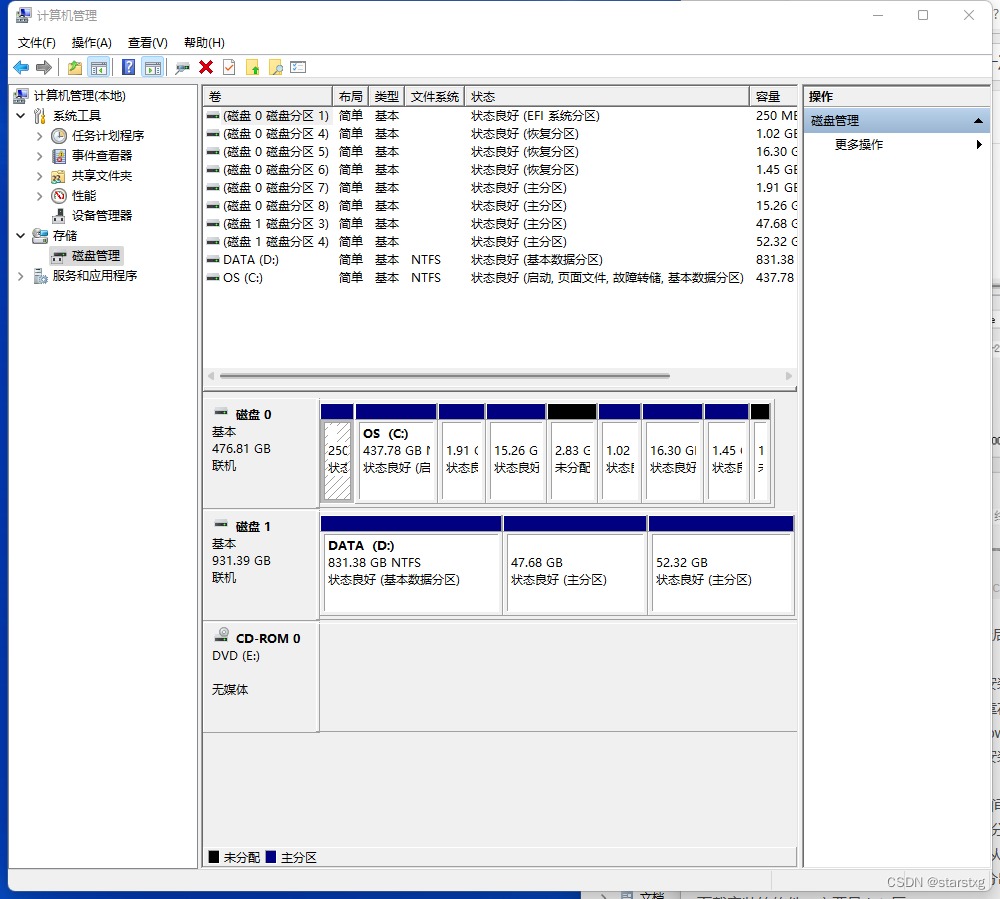
\includegraphics[width=0.75\textwidth]{linux1.png}
\caption{Windows 磁盘管理界面}
\label{fig:linux1}
\end{figure}
接下来选择一个剩余空间较大的普通数据卷，右击，点击“压缩卷”，等待计算完成后，界面会显示当前可用的压缩空间大小。输入你要留给 Ubuntu 的空间量，注意这里的单位标为 MB，规划时可以按约 $1024$ MB 对应 $1$ GiB 换算。图中的 $102400$ 约为 $100$ GiB，只是这台电脑的选择，不用照抄。课程代码本身占用不大，但后面的图像数据集，项目工程以及各类环境会很快长大，有条件可以预留约 $200$ GiB，后续空间不够虽然可以扩容，操作起来却有点麻烦。当然，也别为了凑这个数把 Windows 挤得没地方用了。
\begin{figure}[H]
\centering
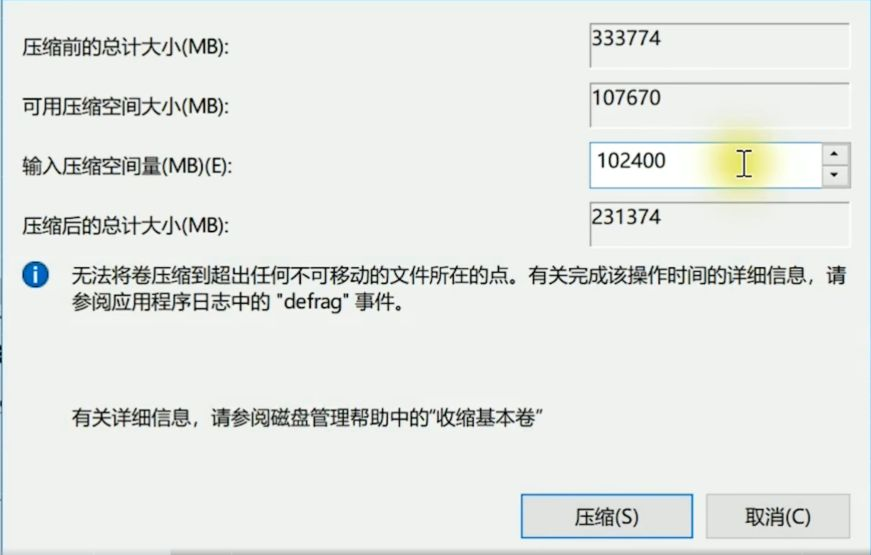
\includegraphics[width=0.75\textwidth]{linux2.jpg}
\caption{压缩卷：读取可压缩空间，再填入自己的容量}
\label{fig:linux2}
\end{figure}
输入好后点击“压缩”，压缩完成后出现一个“未分配”的区域，就说明这一步完成了。\textbf{把它留在未分配状态，不要在 Windows 中新建卷或格式化}，我们等会儿交给 Ubuntu 安装器来处理。如果压缩不到预期大小，先记录界面的限制和现有布局，不要随手删除旁边的分区来凑空间。
\begin{exercise}\label{ex:v1-partition-plan}
记录本机启动模式、分区表类型、各分区容量及剩余空间，规划 Ubuntu 的挂载点与容量。指出已有 ESP 和绝不能格式化的 Windows 分区。
\end{exercise}

\subsubsection{制作启动盘}
首先需要一只容量至少 16 GB 的 U 盘，请先对其中的文件进行备份，后续写入镜像会清空这个 U 盘。

然后进入 Ubuntu 官网下载镜像，下载链接为 \url{https://releases.ubuntu.com/22.04/}。本节截图对应 22.04.5，注意选择 Desktop amd64 的 ISO 文件，不要误下成服务器版。下载好后，我们再按同页的 SHA256SUMS 核对一下文件，具体方法可以看\href{https://ubuntu.com/tutorials/how-to-verify-ubuntu}{Ubuntu 官方镜像校验教程}。ISO 是\textbf{镜像文件}，不是解压后把里面的文件复制到 U 盘就能启动的普通压缩包，所以可别傻傻的直接解压复制。

镜像下载好后，还需要一个启动盘制作器把它写入 U 盘。这里介绍操作比较直观的 balenaEtcher，你也可以按对应说明使用 Rufus 等其他工具。balenaEtcher 的下载链接为 \url{https://etcher.balena.io/}。

安装后点击“Select image”（新版可能叫“Flash from file”）选择刚刚下载的 Ubuntu 镜像，随后在“Select target”中选择你的 U 盘。\textbf{这时候再核对一次设备名和容量，确认没有选到移动硬盘或其他资料盘}，最后点击“Flash!”。等待写入和校验都完成，再安全弹出 U 盘，这样启动盘就做好了。
\begin{figure}[H]
\centering
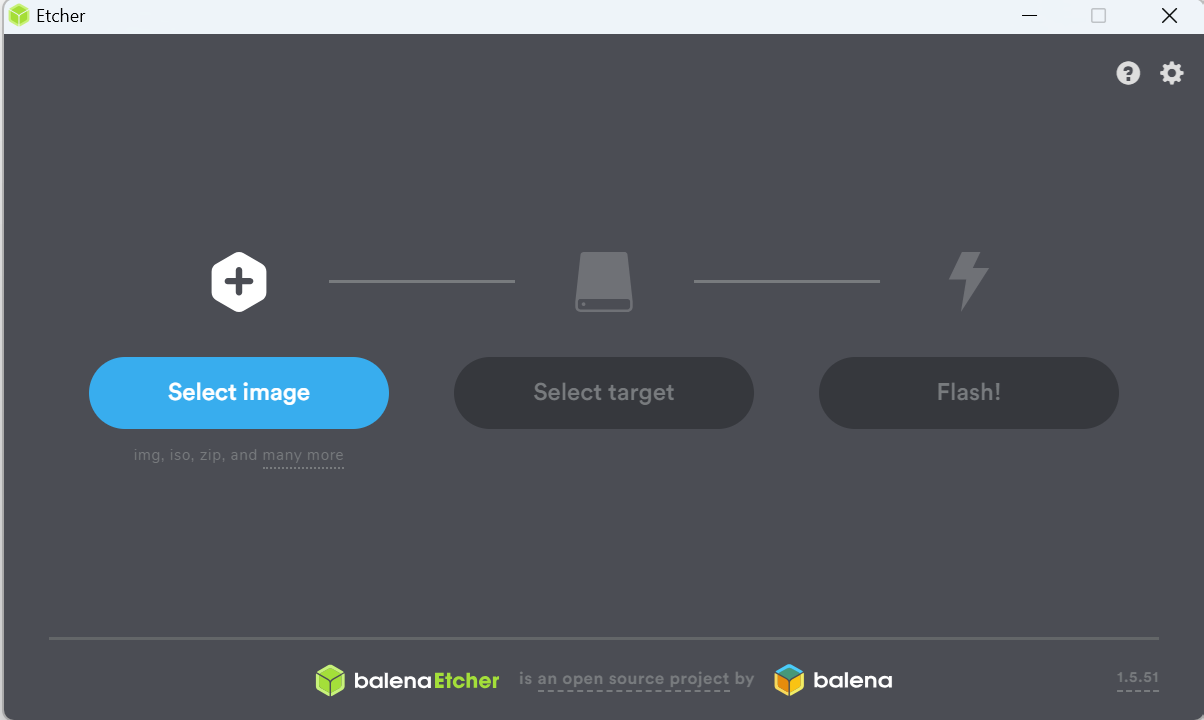
\includegraphics[width=0.8\textwidth]{linux3.png}
\caption{Etcher 界面：镜像、目标盘与写入三个入口}
\label{fig:linux3}
\end{figure}
启动盘做好后，再插到 Windows 中，可能会弹出“需要格式化”的提示。这一般是因为 Windows 不能识别其中所有分区，\textbf{取消提示就好，不要为了消除弹窗把启动盘格式化}，不然你就要重头再来了。这种镜像写入方式也不保证剩余空间还能继续存普通文件，所以资料另找地方放。启动盘被称为“数字生命”，请好好保存，如果后续系统出问题了需要重装，你还用得到它。
\begin{exercise}\label{ex:v1-usb-image}
核对下载的 ISO 校验值，记录 Etcher 中的镜像名称、目标容量及写入校验结果。
\end{exercise}

\subsubsection{从 U 盘进行安装}
插入之前做好的启动盘，接下来我们要让电脑从它启动。在 Windows 中可以按住 Shift 点击“重启”，然后进入“疑难解答”→“高级选项”→“UEFI 固件设置”；也可以重启时按电脑手册里写的快捷键，进入一次性启动菜单。各个主板的按键不太一样，先查清楚再按，否则你可能得“脸滚键盘”了。

\begin{figure}[H]
\centering
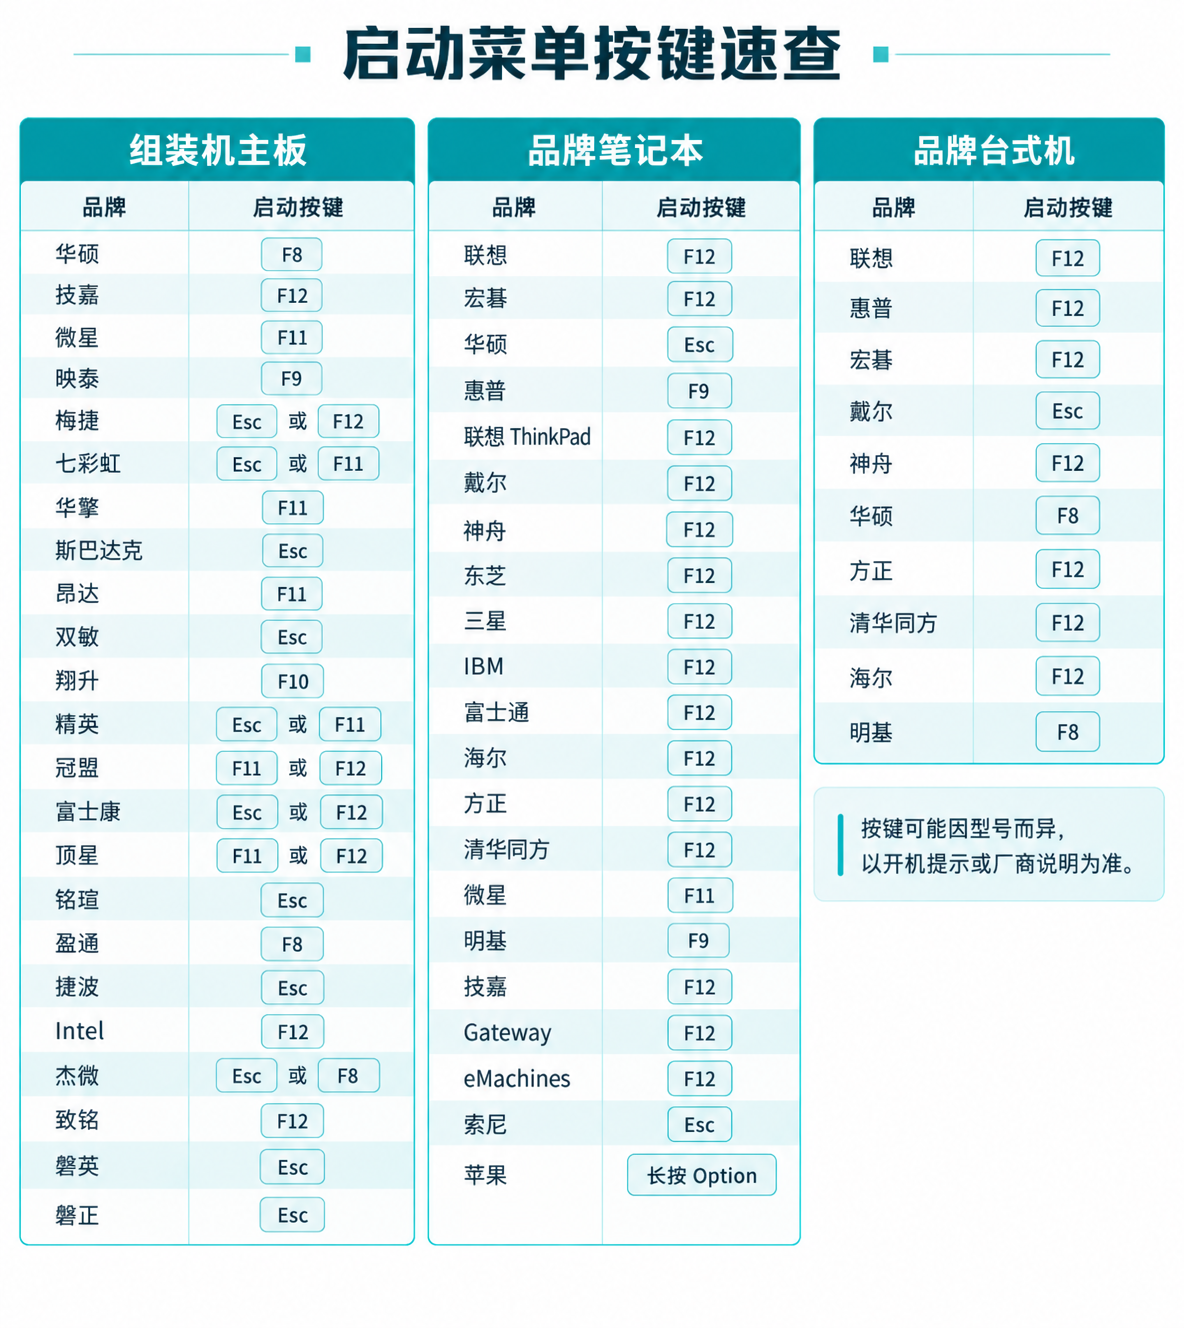
\includegraphics[width=0.8\textwidth]{install1_revised.png}
\caption{启动菜单按键速查}
\label{fig:install1}
\end{figure}

进入启动选项界面后，选择这只 U 盘对应的 UEFI启动项，回车。它可能显示为 Linpus lite，也可能是 Kingston、SanDisk 等品牌名，认准自己的 U 盘即可，不必纠结名字是否和截图一致。接着选择 Install Ubuntu，开始正式安装。

\begin{figure}[H]
\centering
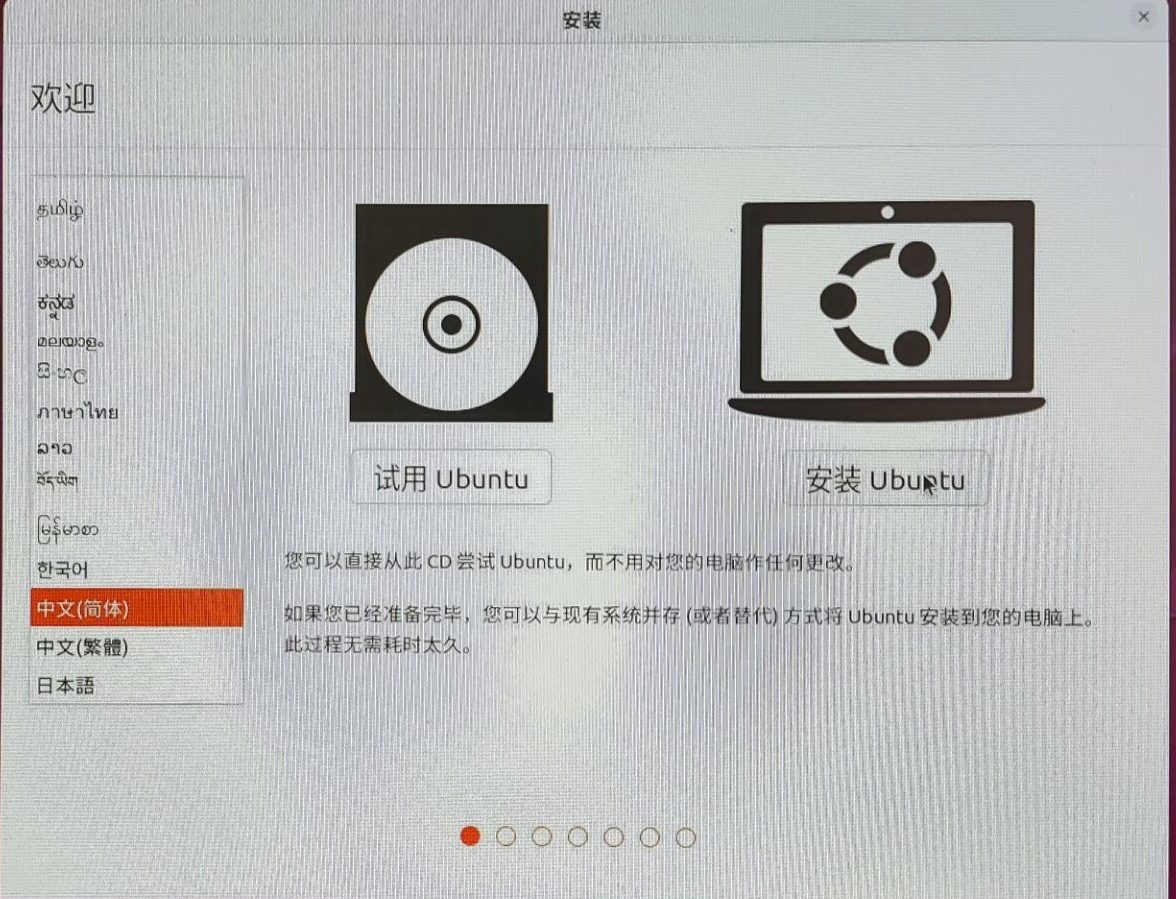
\includegraphics[width=0.75\textwidth]{install2.jpg}
\caption{安装 Ubuntu}
\label{fig:install2}
\end{figure}

首先选择语言为简体中文，“键盘布局”按你实际使用的键盘选择，无线连接和更新可以按当前网络条件决定。然后在“更新和其他软件”页面选择“正常安装”，按硬件需要勾选第三方驱动。
\begin{figure}[H]
\centering
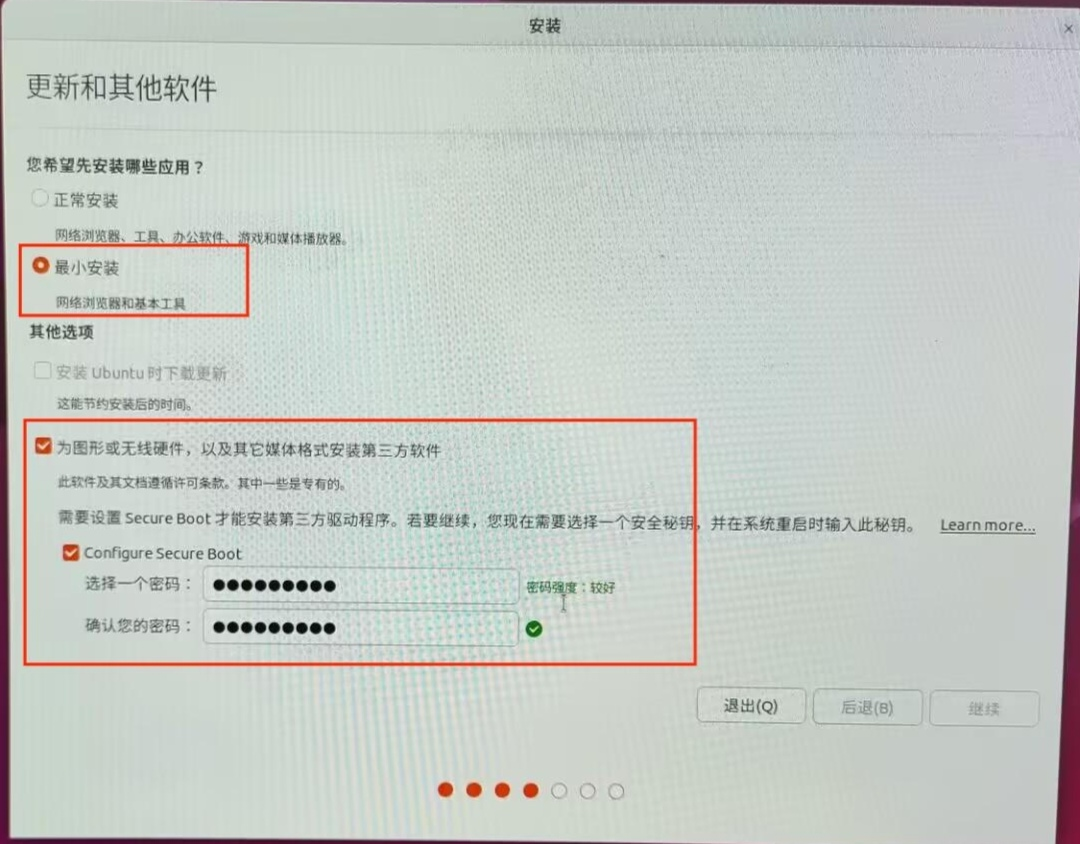
\includegraphics[width=0.75\textwidth]{install3.jpg}
\caption{第三方驱动与 Secure Boot 设置}
\label{fig:install3}
\end{figure}
如果启用了 Secure Boot，安装第三方驱动时可能要求你设置 MOK（Machine Owner Key，机器所有者密钥）注册密码。这个密码是给重启后的密钥注册用的，记下来，到时候按提示确认即可。它不是 Ubuntu 账户的登录密码，后面我们还要另外建立账户，别看到这里填过密码就把后面的步骤跳过去了。

接下来来到“安装类型”，本教程选择\textbf{“其它选项”}，这样我们可以按照刚才的规划手动分区，也能看清究竟要格式化哪些地方。有的安装器会提供“与 Windows 共存”的自动方案，你可以按实际情况选择，但最后的写盘摘要一样要核对。这里最需要注意的是：\textbf{千万不能选择抹掉整个磁盘}，否则留下来的就不是双系统了，到时候只能对着消失的Windows哭泣，重装整个Windows系统。
\begin{figure}[H]
\centering
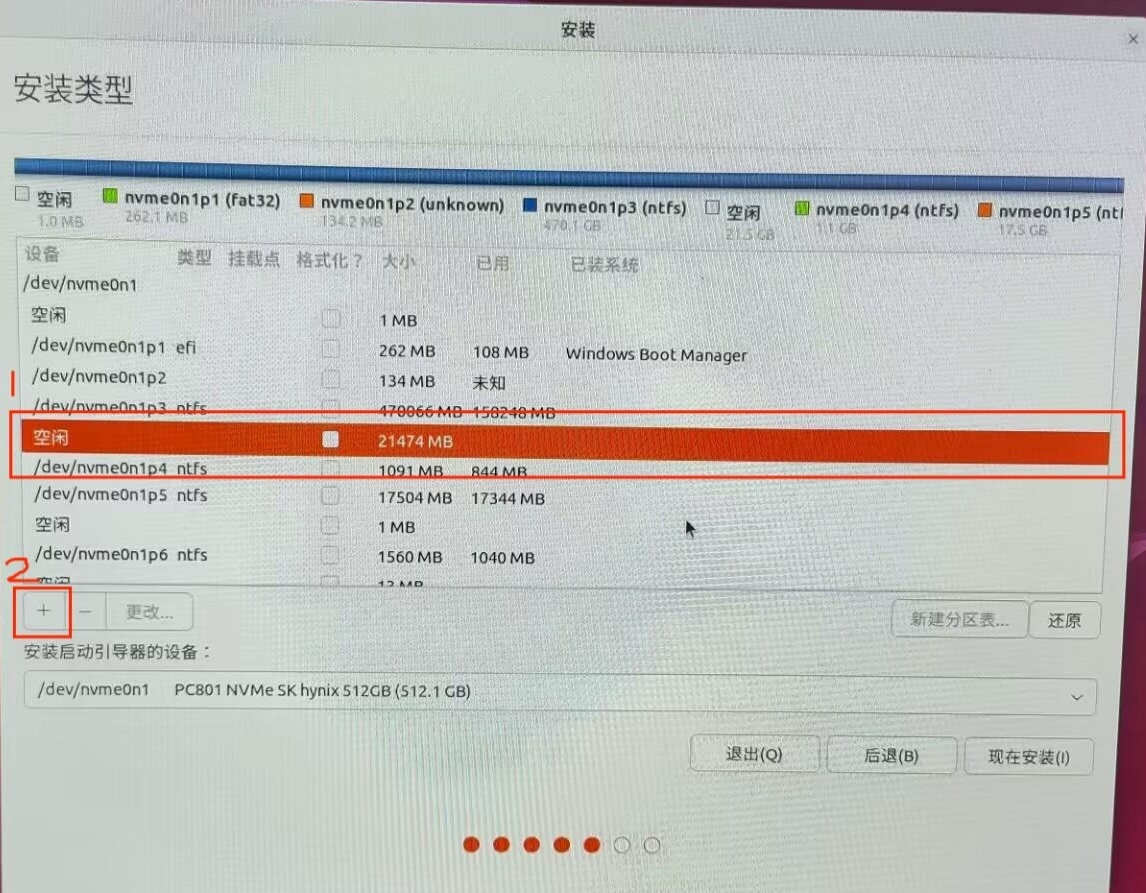
\includegraphics[width=0.8\textwidth]{install4.jpg}
\caption{手动分区：找到之前腾出的空闲空间，图中的设备编号不能照抄}
\label{fig:install4}
\end{figure}
首先找到电脑已有的 EFI 系统分区（EFI System Partition，ESP），它通常是 FAT32，里面有 Windows Boot Manager。我们复用它作为 \texttt{/boot/efi}，\textbf{不要勾选格式化}，Windows 也要靠它启动。这里的 ESP 和存放 Linux 内核的 \texttt{/boot} 不是同一个东西，名字看起来相近，却不能互相替代。如果你的电脑有多块硬盘，需要选择你安装 Ubuntu 的那块硬盘上的 ESP。

然后找到之前压缩出来的空闲区域，点击加号，在这里创建 Ubuntu 的 ext4 分区。你可以按下面两种思路来安排：
\begin{itemize}
\item \textbf{全部放在根分区里。}只创建一个挂载到 \texttt{/} 的分区，用户文件也就放在这个分区里的 \texttt{/home} 目录。这种方式最简洁，适合先把系统用起来；不过日后格式化根分区时，个人文件也会一起被清空。
\item \textbf{把根分区与个人文件分开。}可以给 \texttt{/} 约 80 GiB，再把剩余空间给独立的 \texttt{/home}。这个容量只是例子，你可以按需求调整。以后重装时可以选择保留 /home，不过仍然要先备份，并在安装器里\textbf{明确取消它的格式化}。
\end{itemize}
普通入门安装一般不需要另建 \texttt{/boot}。交换空间（Swap）则可以用安装器建立的交换文件；如果你选择单独建立交换分区，类型选“交换空间”即可。一般来说可以为其分配约 8或16 GiB，或者按电脑内存大小来定。

如果你看过一些旧教程，可能还记得“先分逻辑分区，再分主分区”的说法。不过本节使用的是 GPT，并不按 MBR 的主分区、逻辑分区来安排，也没有这个先后规则。UEFI 的引导文件写入 ESP，\textbf{不要把某个 /boot 分区当作通用的引导安装目标}。如果电脑有多块硬盘，还要看清安装器究竟选中了哪个 ESP；不确定时请学长一起检查，这里多花几分钟，总比装完再抢救省事。相关说明见 \url{https://help.ubuntu.com/community/UEFI}。

\begin{conclusion}
启动模式、分区表、文件系统、挂载点分别管不同的事：UEFI 是怎样启动，GPT 是怎样记录分区，ext4 是怎样存文件，\texttt{/} 与 \texttt{/home} 是从哪里访问文件。已有 ESP 要保留，是否拆分 /home 只影响管理方式，不能代替备份。
\end{conclusion}
\begin{exercise}\label{ex:v1-installer-review}
在纸面方案中给每个分区标记“保留/格式化”及挂载点，并解释 ESP、/boot、swap 的区别。
\end{exercise}

分区安排好后，先别急着点“现在安装”，我们再看一遍写盘摘要：Windows 数据分区和 ESP 都不应该出现在格式化清单里，要格式化的是这次新建的 Ubuntu 分区。确认没有问题后再继续。分区完成后，安装最难的一步就结束了，下来只需要选择时区、账户名和登录密码，等待系统安装完成就好了。

出现安装完成的提示后点击“现在重启”，等到屏幕提示“Please remove the installation medium, then press ENTER”时，拔掉启动盘并按回车。先试着进入 Ubuntu，再重启一次确认 Windows 也能进入；在 Ubuntu 中运行 \texttt{findmnt /} 与 \texttt{findmnt /boot/efi}，看看实际的来源分区和挂载点是否符合规划。两套系统都能正常启动，至此安装就全部完成啦。接下来你可以慢慢按自己的习惯配置，不必第一天就把桌面折腾成最终形态。
\begin{note}
安装完毕后，如果电脑直接黑屏，先别急着判定系统装坏了，一般来说这里最常见的是开了独显直连导致的兼容性问题，大家在BIOS中选择混合模式重启电脑即可。不过如果这样没有好转，也别慌，我们先看它在哪一步黑屏：固件画面、引导菜单，还是登录以后？再确认能否进入 TTY，记下报错和硬件型号。接着按机型手册或 Ubuntu 恢复选项检查显卡模式与驱动，必要时请学长协助。不要未经核对就改 Secure Boot、磁盘模式或删除分区来试错。这里学长曾经遇到过一个同学因为 Secure Boot 关闭后，Bitlocker 保护的 Windows 分区无法解锁，导致 Windows 进不去的情况。但是那个同学以为 Windows 完全没救了，直接把整个磁盘格式化了，结果 Windows 也没了。
\end{note}

\subsubsection{系统设置相关}
\label{sec:ubuntu-boot-order}
Ubuntu 安装完成后，有些电脑会默认先进入 Ubuntu 的引导菜单。如果你平时用 Windows 更多，不想每次开机都手动选，我们有一种比较简单的办法：让电脑默认启动 Windows，只在需要 Ubuntu 时主动选择它。

首先再次进入 UEFI 固件设置，找到 Boot 相关页面，把 Windows Boot Manager 移到 ubuntu 上方，保存退出即可。保存前记得拍下原来的顺序，改完后再分别测试两套系统能否启动。要用 Ubuntu 时，从一次性启动菜单中选择 ubuntu 就好。

这里顺便区分一下：固件的启动顺序决定先启动哪个引导程序，GRUB 菜单的默认项则决定进入 GRUB 引导程序后选哪个系统，它们是两层设置。如果你觉得每次打开一次性启动菜单还是繁琐，也可以在 GRUB 中设置默认项，下面的美化小节会接着说明。
\begin{exercise}\label{ex:v1-boot-order}
进入固件设置，只记录当前启动顺序与调整入口，不保存修改。说明一次性选择 Ubuntu 与永久调整默认顺序分别适合什么情况。
\end{exercise}

\subsubsection{系统扩容*}
\label{sec:ubuntu-resize}
如果系统里的文件已经多到空间不足了，我们可能就要给 Ubuntu 扩容。不过先别急着动分区，用 \texttt{df -hT /} 看看是不是根分区真的满了，再用 \texttt{du -h --max-depth=1 路径} 找出空间花在哪里。如果只是某些你的个人数据越来越大，把它迁移到另一个位置，往往比移动系统分区省事。

确实需要扩容时，我们可以用 GParted 分区管理工具。上面介绍过 Windows 下的磁盘管理，这里就换换口味，看看 Ubuntu 下怎样操作。\textbf{动手前先备份，并确认供电可靠}，移动分区可能要等很久，中途断电或强制退出都有损坏数据的风险。
\Needspace{12\baselineskip}
\begin{example}[观察根分区]
Ubuntu 中安装 GParted 后打开，只查看布局：


\Needspace{7\baselineskip}
\begin{tbash}
sudo apt update
sudo apt install gparted
sudo gparted
\end{tbash}


按磁盘型号选择设备，记录根分区和相邻未分配空间。
\end{example}
\begin{figure}[H]
\centering
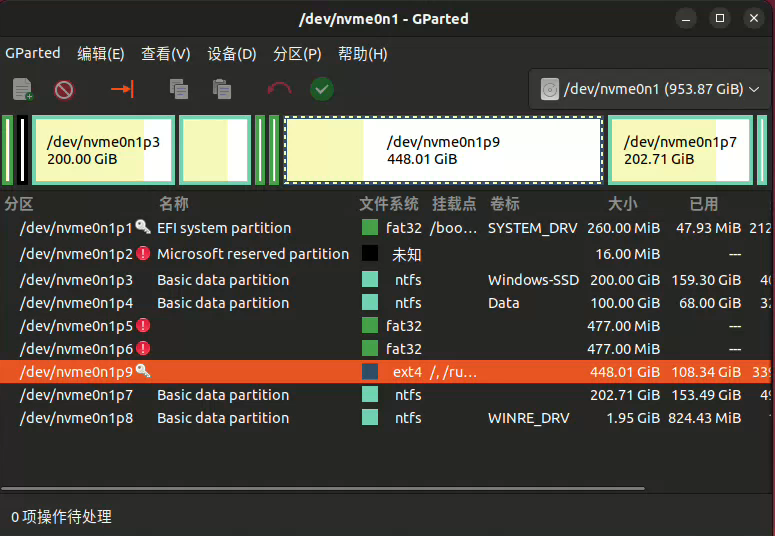
\includegraphics[width=0.85\textwidth]{linux10.png}
\caption{GParted}
\label{fig:linux10}
\end{figure}
\begin{figure}[H]
\centering
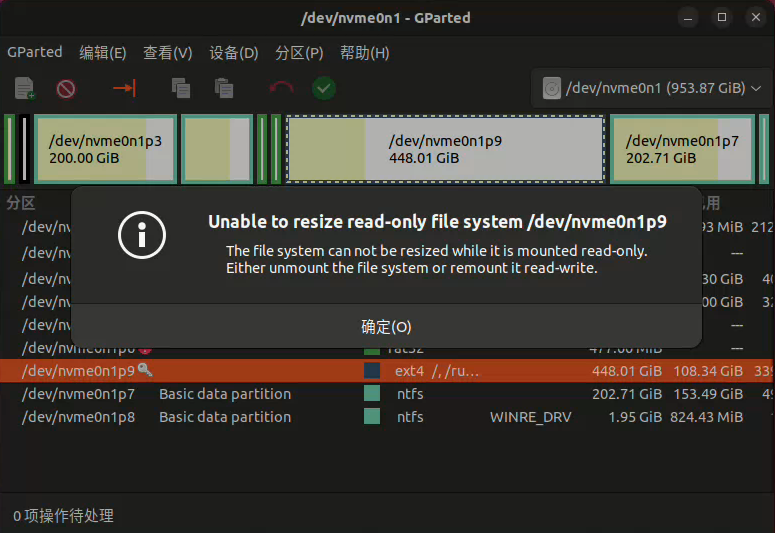
\includegraphics[width=0.85\textwidth]{linux9.png}
\caption{提示 “只读文件系统无法调整大小”}
\label{fig:linux9}
\end{figure}
但是如果这个时候你直接选择扩容，会发现有报错。为什么不能直接调整大小呢？因为当前 Ubuntu 的系统分区正在使用，通常要到另一个环境里才能移动。

这时候我们可以拿出安装时做好的启动盘，按之前的方法进入 Try Ubuntu。选择试用后，打开终端和 GParted，确认目标分区没有挂载，再按计划操作。扩容还需要合适位置的相邻未分配空间；如果中间隔着其他分区，就可能要移动它们，风险和耗时也会增加。\textbf{不要先在正在运行的系统里调节 swap 或其他分区位置}，担心的话先把完整计划交给学长核对，再到 Live 环境执行。

等待操作完成后重启，用 \texttt{lsblk} 和 \texttt{df -hT /} 分别核对分区容量与文件系统容量。它们看的不是同一层，只看一个数字变大还不够。具体限制可以查 \url{https://gparted.org/display-doc.php?name=help-manual}。
\begin{exercise}\label{ex:v1-resize-plan}
画出“根分区—其他分区—未分配空间”的布局，说明为何不能直接扩大根分区。写出备份、离线环境和结果核验计划。
\end{exercise}

\subsubsection{GRUB 美化*}
\label{sec:grub-theme}
也许你已经看腻了启动时那个黑框框，想把它换得好看一点。那我们接下来就给 GRUB 换个主题，不过先把两个系统都能启动这件事确认好，再来折腾外观。主题负责“长什么样”，默认进入哪个系统则要另外设置，装好主题不会顺手替你把这件事也做了。

下面展示的是 Tela 主题，对应项目在 \url{https://github.com/vinceliuice/grub2-themes}。在介绍 Git 之前，你可以先点击网页上的 Code → Download ZIP 下载。然后打开 README，按当前版本的说明选择主题名和分辨率参数；安装脚本也先读一遍，看看要改哪些文件，再决定是否执行。装其他主题的时候也要类似检查，别把来历不明的脚本直接交给 sudo，桌面颜值还没上去，启动先出问题就不划算了。
\Needspace{8\baselineskip}
\begin{example}[保存配置后检查默认项]
在 Ubuntu 中先保存原配置，再只读查看实际菜单标题：


\Needspace{7\baselineskip}
\begin{tbash}
sudo cp -a /etc/default/grub /etc/default/grub.before-training
grep '^GRUB_' /etc/default/grub
grep "^[[:space:]]*menuentry " /boot/grub/grub.cfg
\end{tbash}


如果你还希望没有操作时自动进入 Windows，我们就小小地配置一下引导。打开 \path|/etc/default/grub|，找到 \texttt{GRUB\_DEFAULT}，把它设为\textbf{本机实际菜单标题或稳定的菜单项 ID}。不过一般来说 Windows 是第三项。改完后运行 \texttt{sudo update-grub} 生成配置，确认没有报错；\texttt{grub.cfg} 是它生成出来的文件，别直接编辑。
\end{example}
\begin{note}
主题安装和引导配置改错可能妨碍选择启动项，所以记得保留可启动 U 盘和原配置。配置有误但 Ubuntu 仍能启动时，至少还可以按对应备份恢复并重新生成：


\Needspace{6\baselineskip}
\begin{tbash}
sudo cp -a /etc/default/grub.before-training /etc/default/grub
sudo update-grub
\end{tbash}

只有确认备份对应本次改动才恢复，别覆盖后来有意修改的配置。
\end{note}
\begin{figure}[H]
\centering
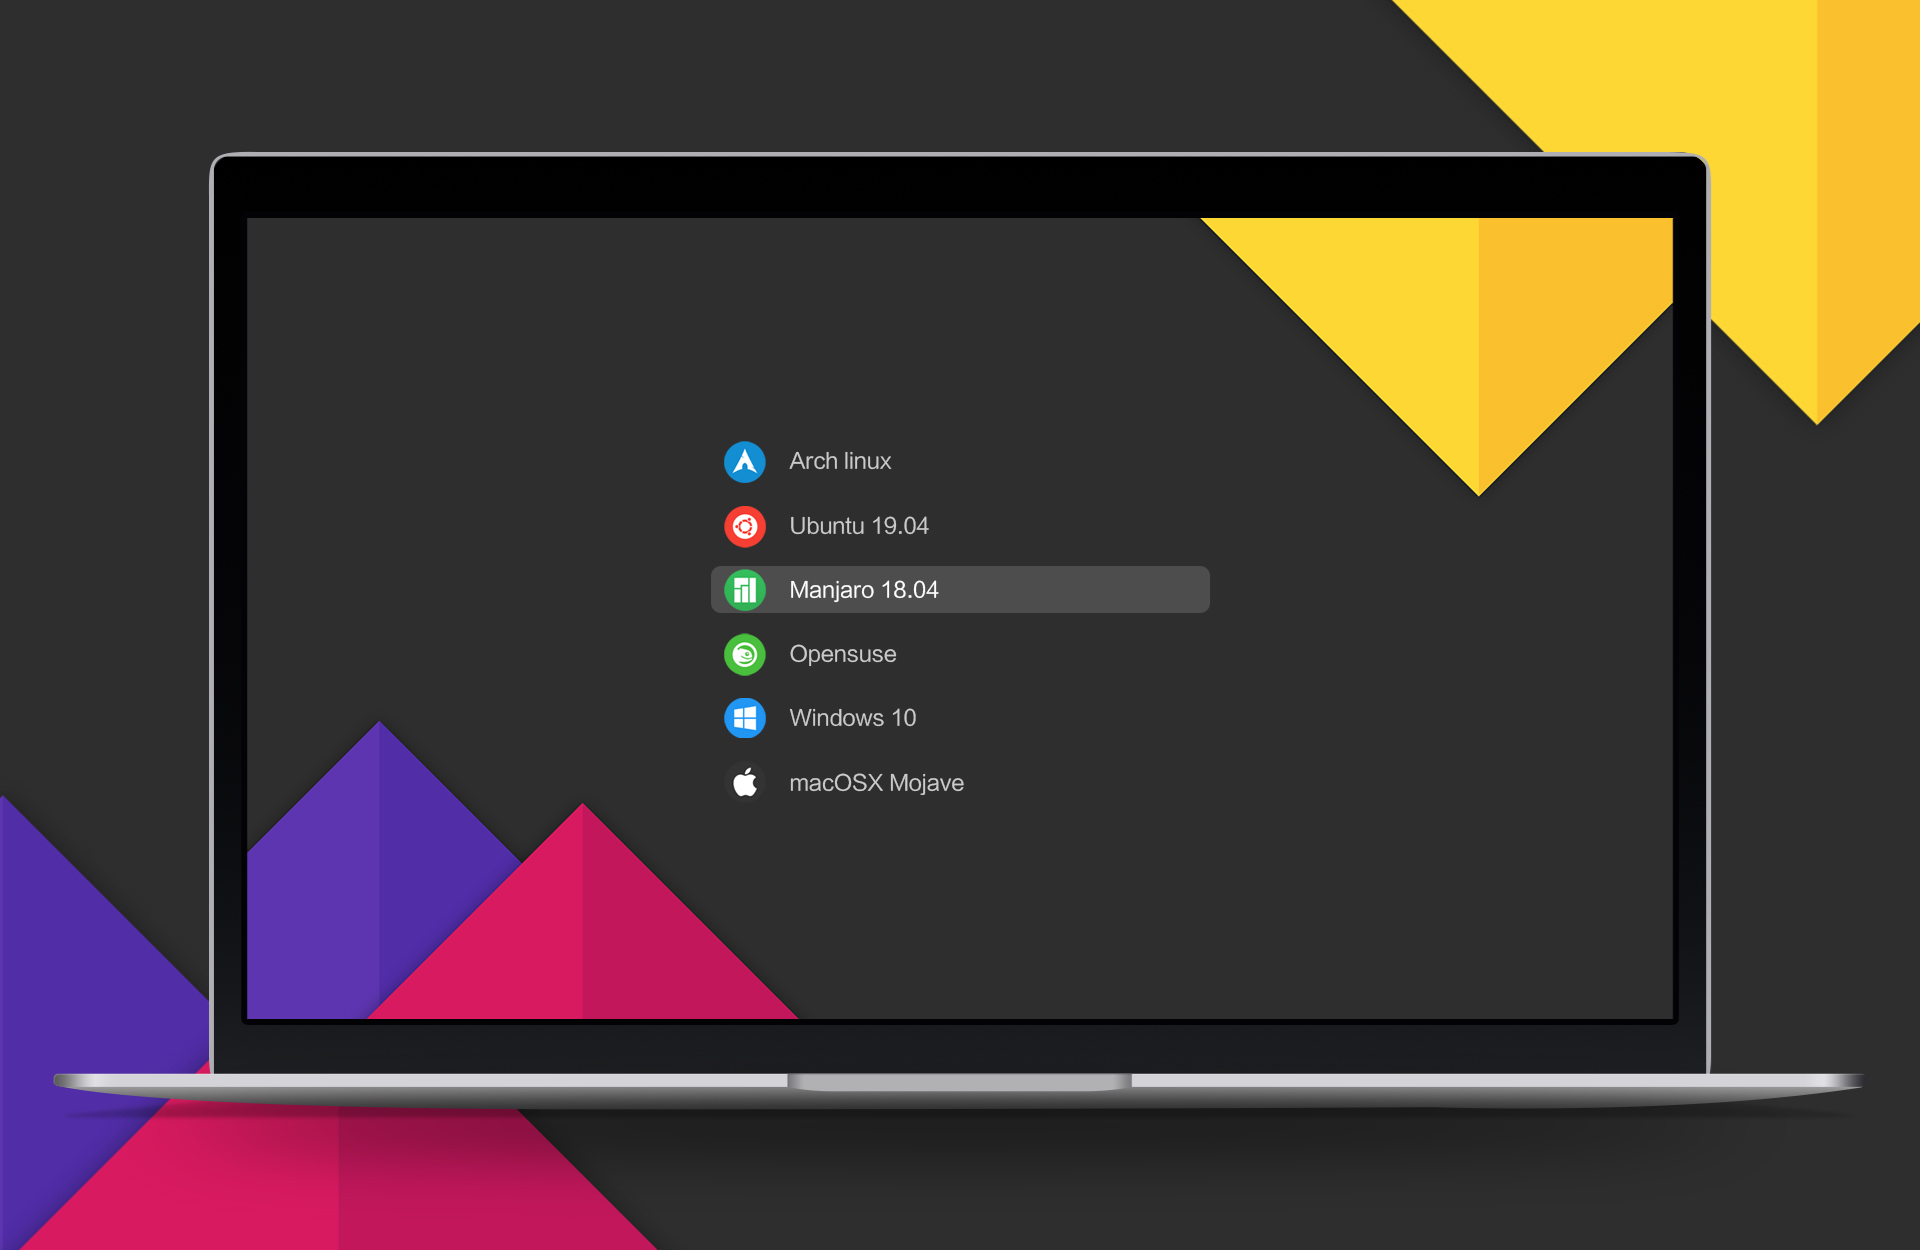
\includegraphics[width=0.8\textwidth]{grub.png}
\caption{Tela 主题效果示例}
\end{figure}

\subsubsection{桌面美化*}
\label{sec:gnome-customize}
GRUB 好看了，桌面也可以按自己的喜好收拾一下。Ubuntu 22.04 默认使用 GNOME，换个主题、装几个顺手的插件，就能让桌面更合你的习惯。

我们先分清要装的东西：主题主要改窗口外观，图标包改应用图标，Shell 扩展则增加桌面功能。它们各管一层，所以装了图标包，窗口颜色没变是正常的。先记下原来的外观，每次改一项，出了问题也更容易撤回。
\Needspace{8\baselineskip}
\begin{example}[主题的下载]
这里推荐一个美化网站 GNOME LOOK \url{https://www.gnome-look.org/browse/}，可以从这里挑选自己喜欢的主题(Gnome Shell Themes)或图标包(Full Icon Themes)下载，解压到用户目录。然后借助 Tweaks（优化）和Extension Manager（扩展管理器）进行美化的管理。下面的压缩包名要换成自己实际下载的文件名：


\Needspace{8\baselineskip}
\begin{tbash}
mkdir -p ~/.themes ~/.icons
tar -tf theme.tar.gz
tar -xf theme.tar.gz -C ~/.themes
sudo apt install gnome-tweaks gnome-shell-extension-manager
\end{tbash}


装好后打开 Tweaks， 在“外观”一栏选择刚装好的兼容主题或图标。有些 GTK4/libadwaita 应用不一定跟着 GTK3 主题改变，不用因为一个窗口没变色就把主题重装一遍。

接下来轮到 Extension Manager 了。打开“浏览”页，搜索你自己喜欢的扩展，点击安装。安装后在“已安装”页可以看到开关和设置按钮，开关控制启用状态，齿轮打开该扩展设置。注意有些扩展需要重启 GNOME 才能生效，可以按 Alt+F2 输入 r 回车重启。
\end{example}
\begin{figure}[H]
\centering
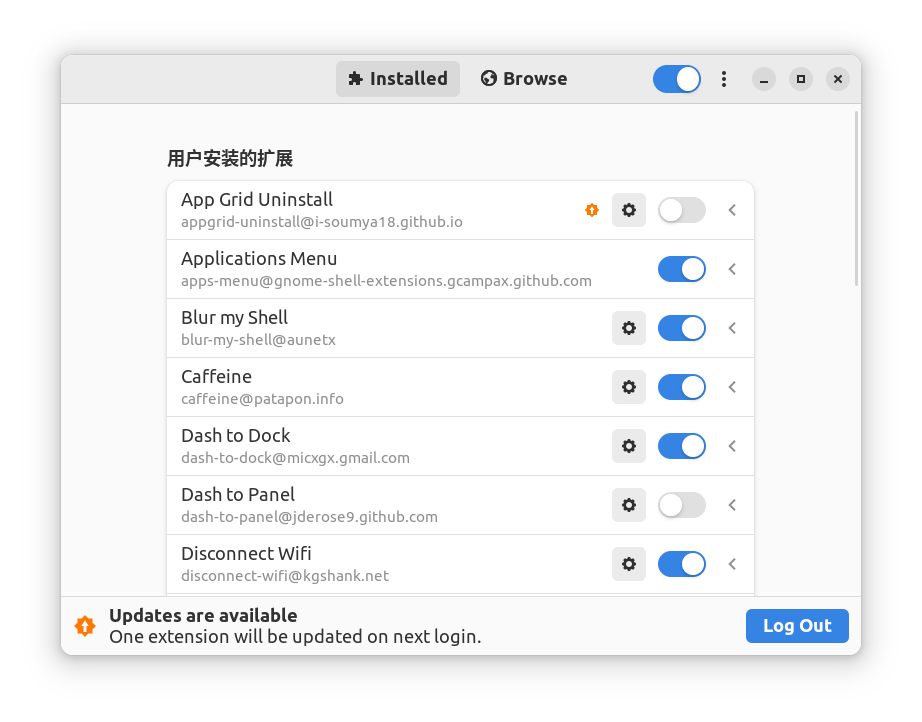
\includegraphics[width=0.8\textwidth]{gnome_extension_manager.png}
\caption{扩展管理器}
\label{fig:extension_manager}
\end{figure}
更多扩展可以在 \url{https://extensions.gnome.org/} 按版本查找。比如 Vitals 可以显示资源占用，Dash to Dock 可以调整程序坞，Clipboard Indicator 可以帮你找回刚刚复制过的文字, Caffeine让屏幕保持唤醒。建议先挑两三个顺手的，别一次全装——插件之间偶尔也会互相打架，尤其是 Dock 和 Panel 类扩展，装多了排查起来很痛苦。

\textbf{常用插件}

以下是视觉组往届同学常用的几款：

\begin{center}
\begin{tabular}{cc}
\toprule[1.5pt]
插件名 & 作用\\
\midrule[1pt]
Caffeine & 保持屏幕常亮，编译、跑数据集时防止自动锁屏\\
TopHat / Vitals & 在顶栏实时显示 CPU、内存、温度等信息\\
Dark Mode Toggle / Night Theme Switcher & 一键或按计划自动切换深色/浅色模式\\
Dash to Dock & 把左侧 Dock 栏变成可自定义的程序坞\\
Dash to Panel + ArcMenu & 合成类似 Windows 的底部任务栏与"开始菜单"\\
Rounded Window Corners Reborn & 给窗口加上圆角\\
Blur my Shell & 给顶栏、Dock 等加上毛玻璃半透明效果\\
Sound Input \& Output Device Chooser & 在右上角菜单直接切换声音输出/输入设备\\
Clipboard Indicator & 剪贴板历史记录，复制过的内容随时找回来\\
\bottomrule[1.5pt]
\end{tabular}
\end{center}

\begin{note}
上表插件的主页链接：

\begin{itemize}
\item Caffeine：\url{https://extensions.gnome.org/extension/517/caffeine/}
\item TopHat：\url{https://extensions.gnome.org/extension/5219/tophat/}
\item Vitals：\url{https://extensions.gnome.org/extension/1460/vitals/}
\item Night Theme Switcher：
\url{https://extensions.gnome.org/extension/2236/night-theme-switcher/}
\item Dash to Dock：\url{https://extensions.gnome.org/extension/307/dash-to-dock/}
\item Dash to Panel：\url{https://extensions.gnome.org/extension/1160/dash-to-panel/}
\item ArcMenu：\url{https://extensions.gnome.org/extension/3628/arcmenu/}
\item Rounded Window Corners Reborn：\par
\url{https://extensions.gnome.org/extension/7048/rounded-window-corners-reborn/}
\item Blur my Shell：\url{https://extensions.gnome.org/extension/3193/blur-my-shell/}
\item Sound Input \& Output Device Chooser：\par
\url{https://extensions.gnome.org/extension/906/sound-output-device-chooser/}
\item Clipboard Indicator：\url{https://extensions.gnome.org/extension/779/clipboard-indicator/}
\end{itemize}
\end{note}

\begin{figure}[H]
\centering
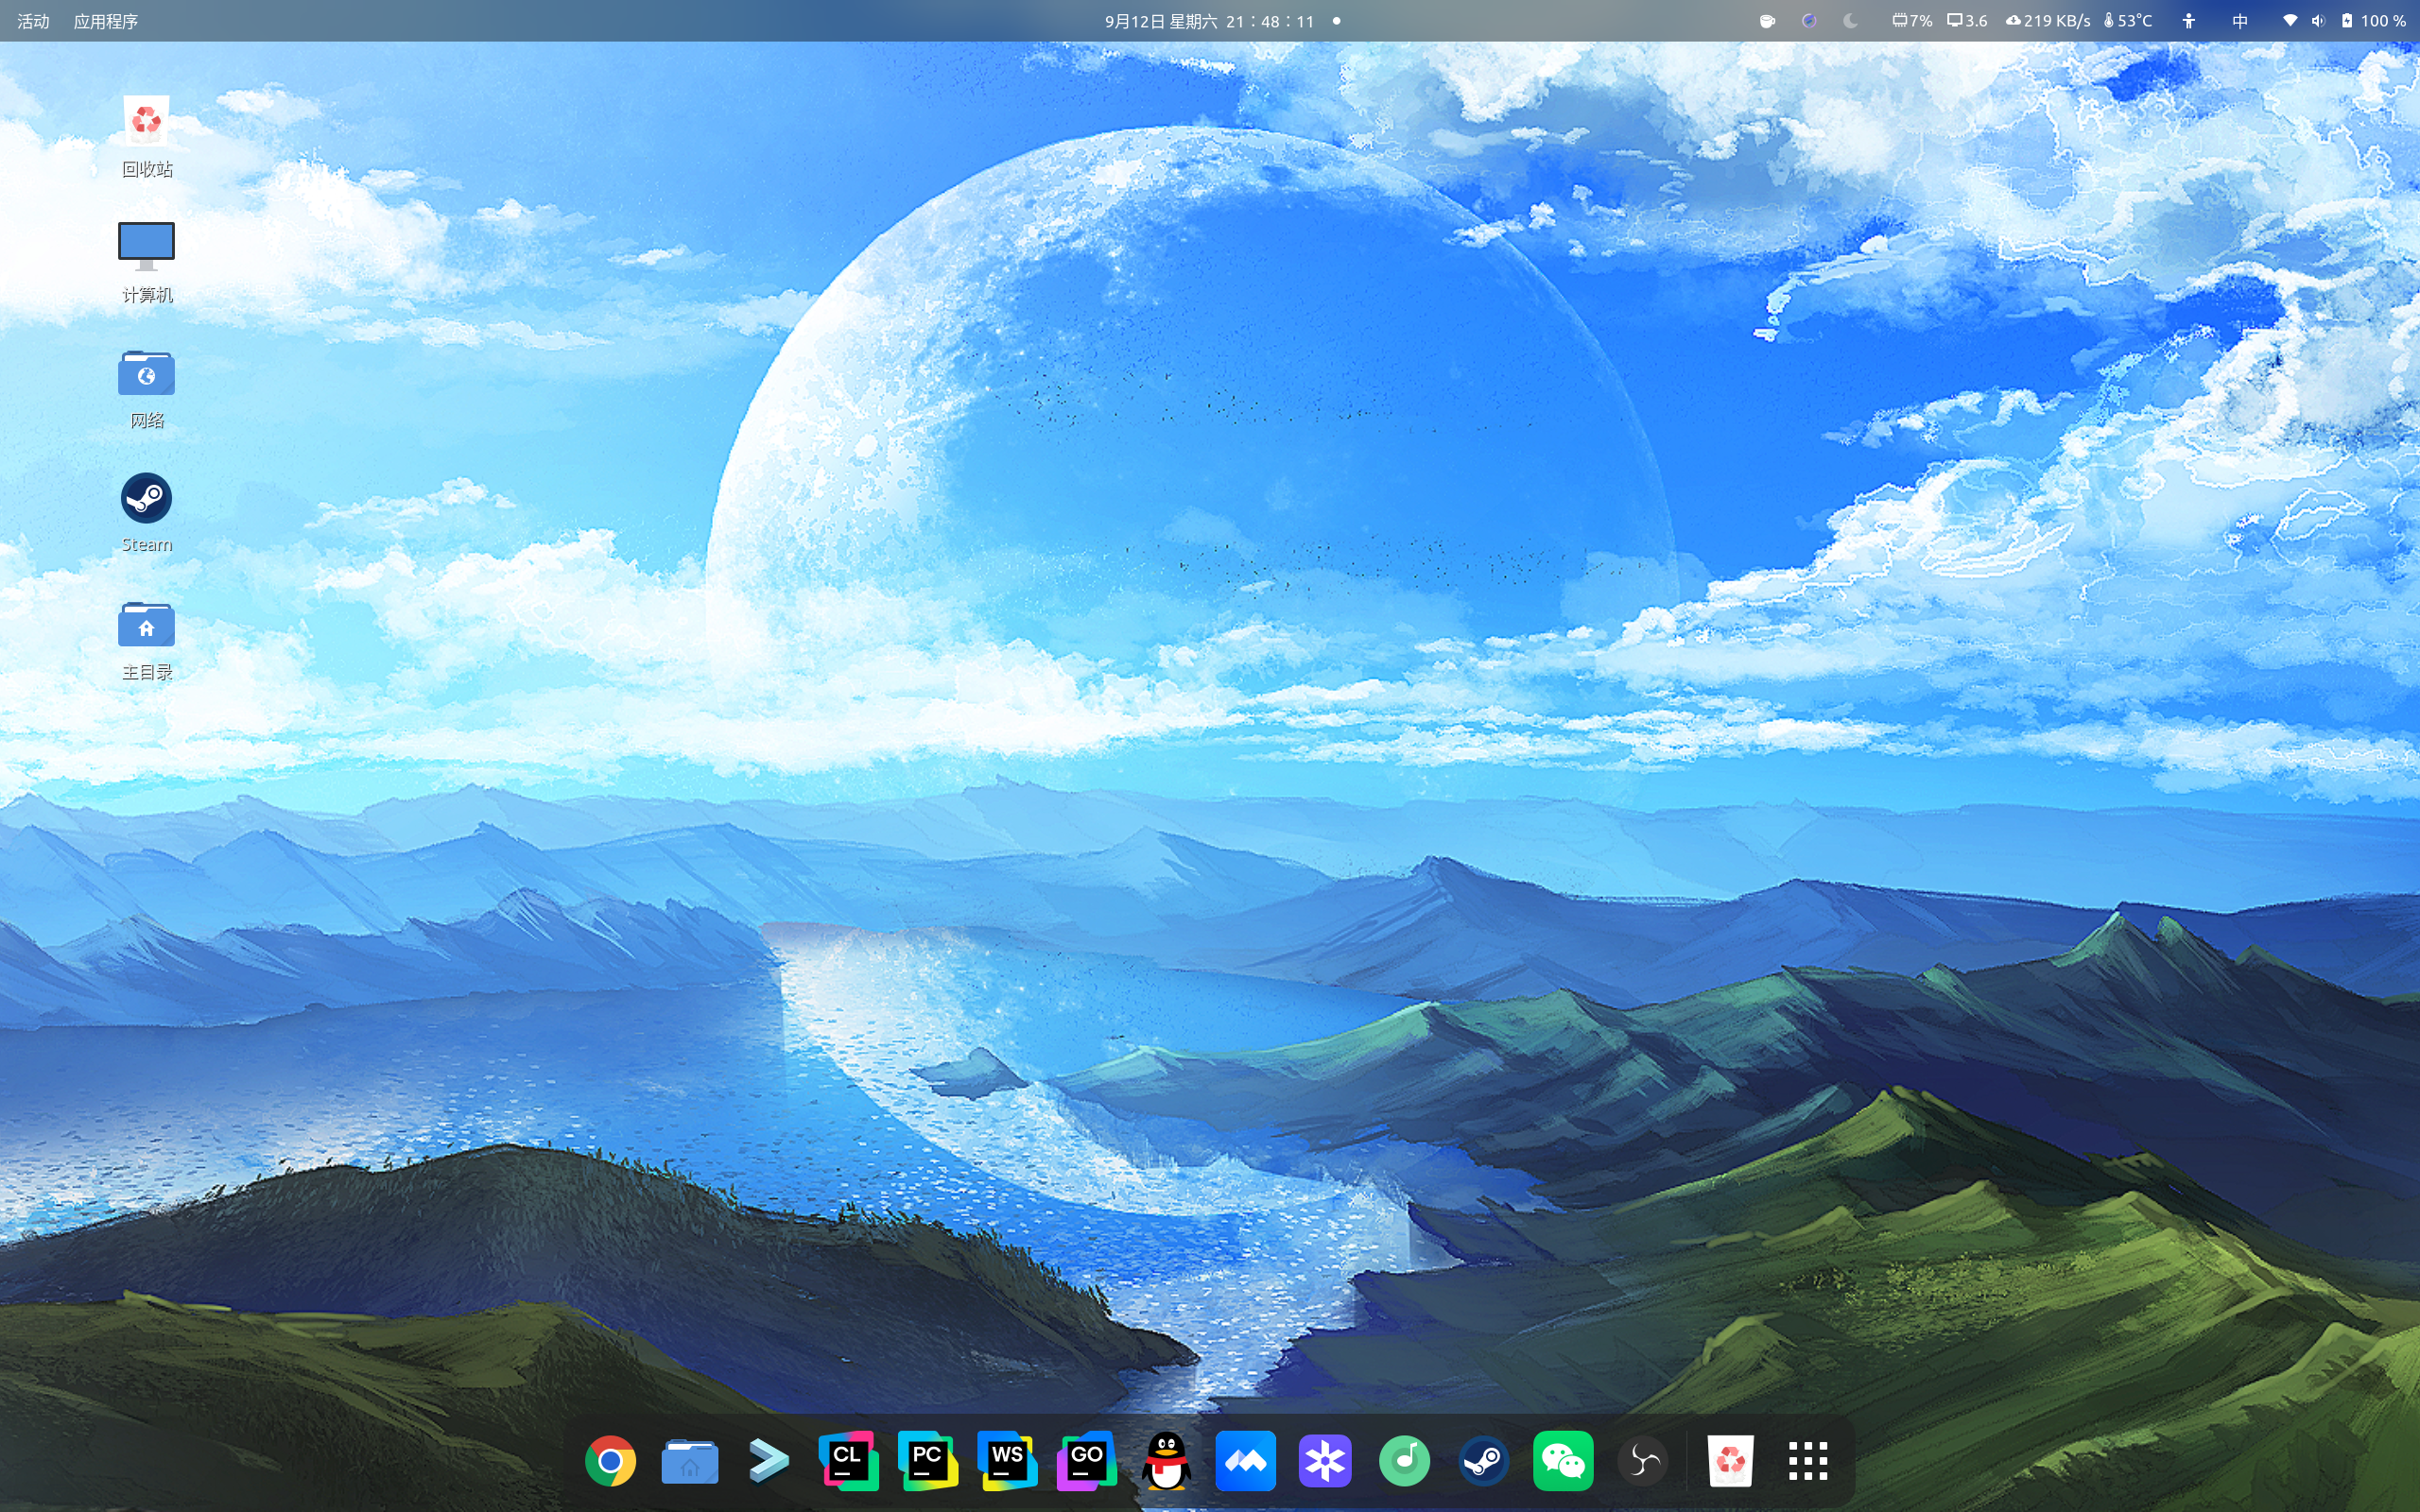
\includegraphics[width=0.85\textwidth]{gnome_desktop_after.png}
\caption{美化后的 GNOME 桌面}
\label{fig:desktop_after}
\end{figure}


\section{系统数据备份*}
配置环境前须完成本节。系统异常时，快照恢复通常优于重装。
恭喜你已经成功安装了 Ubuntu 双系统。作为新手，想来你在刚刚的安装过程中一定很小心，毕竟谁也不想刚装好就出什么差错。不过在后续的工作中，我们还会安装各种各样的软件包、配置各种各样的环境，如果不小心配错了东西，轻则程序找不到，重则系统无法正常工作（简称寄了）。这时候就需要根据问题进入恢复选项、修正配置，实在处理不了才考虑重装。

当然，我们肯定不愿意每次都从头再来，所以很有必要学会备份（Backup）：在大改环境之前存个档，出问题时才有机会回到改动之前。不过系统配置和你写的代码不一定保存在同一份备份里，下面我们先把这个范围分清楚，再试一次恢复。存档到底能不能读，也要试过才知道。
\label{sec:system-backup}

\subsubsection{Timeshift 系统快照}
Timeshift 可以给系统文件和设置制作快照（Snapshot），你可以把它想成给系统照一张相，后来配环境出了问题，再按这张相恢复。操作并不复杂，比事后重新配一遍省事得多；不过相机拍到了什么，还是要看你设置的范围，不是按一下就把整台电脑都保存了。
\begin{note}
\textbf{Timeshift 默认排除个人文件。}源码、照片、数据集要另做备份；快照放在同一块物理盘上，也无法抵御这块盘损坏。恢复会把所选系统文件还原到快照状态，期间的新配置可能被覆盖。先备份个人数据和当前配置，确认目标系统与快照，再恢复。官方说明见 \url{https://github.com/linuxmint/timeshift}。
\end{note}
\Needspace{8\baselineskip}
\begin{example}[创建并核对系统快照]
首先在 Ubuntu 中安装 Timeshift，然后从应用菜单点击它的图标，或者在终端里输入最后一条命令，进入配置向导：


\Needspace{7\baselineskip}
\begin{tbash}
sudo apt update
sudo apt install timeshift
sudo timeshift-launcher
\end{tbash}


进入向导后，首先选择快照类型。我们前面安装的是一般的 ext4 系统，选 RSYNC 即可；它借助 rsync 与硬链接保存文件，未变化的内容可以共享。BTRFS 则利用文件系统本身的快照，但要求受支持的子卷布局，不是看到磁盘格式叫 Btrfs 就一定能用。

然后选择保存快照的位置，按磁盘型号和容量认清目标，并确认它有足够空间、支持 Linux 权限和硬链接。有条件的话，我们可以用另一块盘来保存，这样原来的盘坏了，备份才不至于跟着一起消失。自动备份页面可以选择每月、每周、每天等计划，旁边的数量表示保留多少份；旧快照会按保留策略清理，所以先想好自己要留多久，不必把所有选项都勾上。

接下来读清“用户主目录”和“筛选”页：哪些文件包含在内，哪些排除在外。确认范围后完成向导，点击“创建”，等快照制作完成。我们再用下面的命令查看列表：


\Needspace{5\baselineskip}
\begin{tbash}
sudo timeshift --list
\end{tbash}


列表里应该能找到这次的时间、标签和注释，创建过程也不应该有失败提示。到这里就有了一份系统快照，不过个人代码和数据仍要按照前面的提醒另做备份。完成初始配置后，你也可以直接在命令行创建手动快照，通用形式为 \texttt{timeshift --create [选项]}，比如：


\Needspace{6\baselineskip}
\begin{tbash}
sudo timeshift --create --comments "before-training" --tags O
sudo timeshift --list
\end{tbash}


这里的 \texttt{--comments} 用来写说明，\texttt{--tags O} 表示按需创建。设备选择沿用你刚刚核对过的配置，我们不用照抄别人的磁盘名。
\end{example}
\begin{figure}[H]
\centering
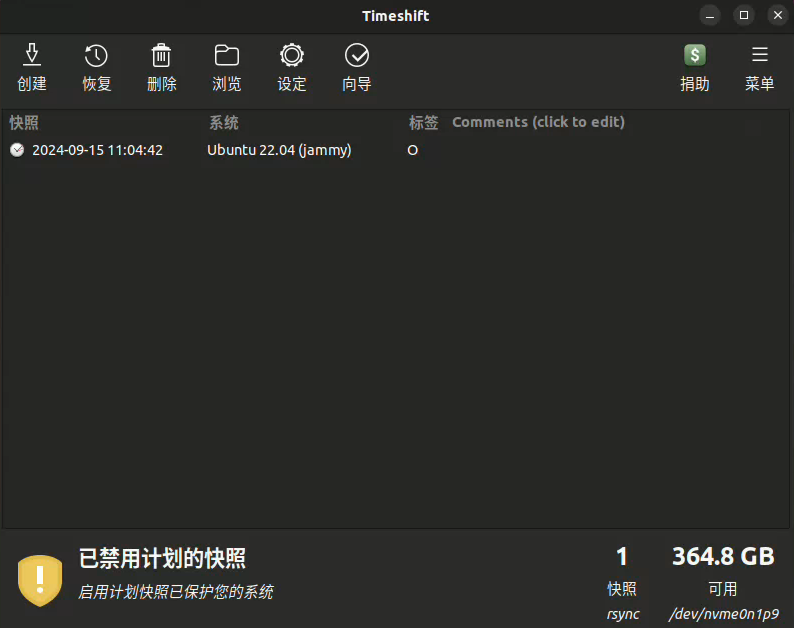
\includegraphics[width=0.8\textwidth]{restore1.png}
\caption{Timeshift 列表：核对时间、系统版本与快照数量；截图不是本次创建结果}
\label{fig:restore1}
\end{figure}

\textbf{接下来我们看看怎样恢复。}如果系统还能正常打开桌面，就启动 Timeshift，选择刚刚核对过的快照，点击“恢复”。这里要特别留意目标设备页：根分区、EFI 分区等映射指的是要恢复到哪里，不只是备份存在哪里。先确认当前文件已经另做备份、目标系统也选对了，再读一遍最终变更摘要，确认后继续。恢复结束后重启，看看被恢复的配置是否回到原来的内容，个人文件是否仍在。
\begin{figure}[H]
\centering
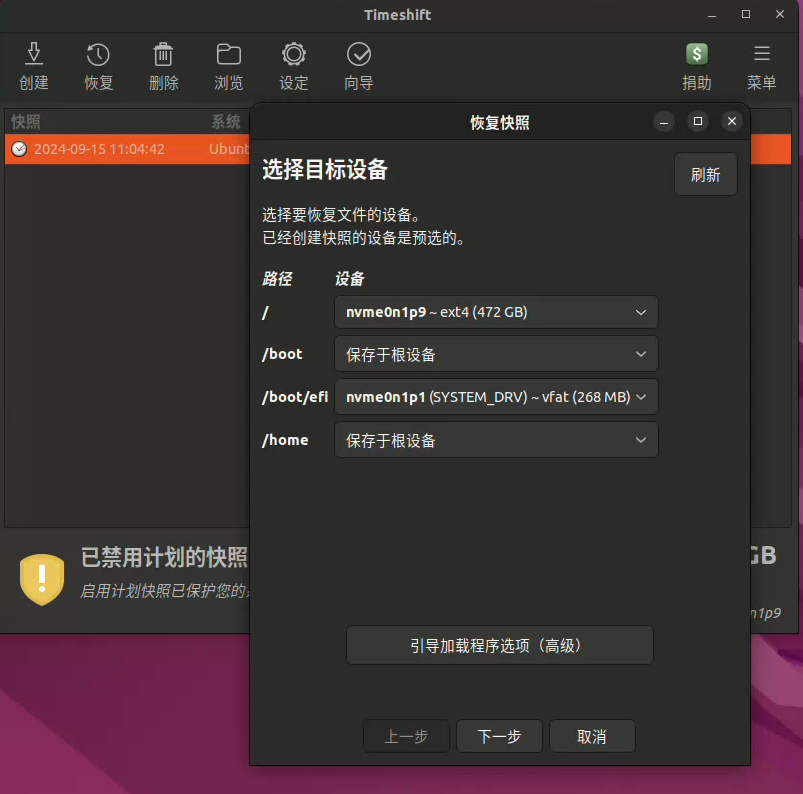
\includegraphics[width=0.75\textwidth]{restore2.png}
\caption{恢复目标选择页：确认的是目标分区，不只是备份保存位置}
\label{fig:restore2}
\end{figure}
如果图形化桌面已经打不开，但还能进入 TTY，可以先运行 \texttt{timeshift --help} 看当前版本的用法，再通过 \texttt{timeshift --restore} 进入交互恢复。如果连系统都进不去了，这时候之前保存的“数字生命”就派上用场了：从 Live U 盘进入 Try Ubuntu，安装 Timeshift，再选择备份所在的设备和要恢复的目标系统。不要为了让命令少问几句，就照抄不明理由的 \texttt{--skip-grub} 跳过引导处理。

我们练习恢复时，优先用虚拟机或可以重建的练习系统：快照前保存一份练习配置，然后改动它，再恢复，看看内容是不是真的变回来了。不用为了交练习把自己正在使用的系统盲目回档；如果暂时没有练习系统，就先记下创建结果和恢复计划，把\textbf{实际系统恢复留作待验证}，等有合适环境再补上。
\begin{exercise}\label{ex:v1-snapshot}
创建一个带注释的快照，记录列表、保存设备和排除范围。说明哪些个人文件仍需另备份；在可重建系统中完成一次配置恢复并记录前后内容，没有该环境时明确待验证项。
\end{exercise}

\subsubsection{文件归档与恢复：先在小目录里练}
\label{sec:archive-backup}
Timeshift 帮我们保存系统状态，那自己写的代码和配置又怎样备份呢？接下来介绍 \texttt{tar}，它可以把多个文件打成归档（Archive），配合 gzip 压缩后，常见的扩展名就是 \texttt{.tar.gz}。这样我们就能把一个目录里的内容打包带走，再解到另一个地方。

不过 tar 归档不是整块磁盘的扇区镜像，它没有自动保存 GPT、EFI 引导状态，也不能保证正在写入的文件前后一致。直接“把 / 打包，再解压到 /”还可能覆盖真实系统，对新手来说既难验证又难补救。所以这里我们先在一个小目录里练清楚备份和恢复的过程；如果以后需要迁移整个系统，再单独准备完整的恢复方案。

通用形式为 \texttt{tar -czf 归档文件 -C 起始目录 要保存的相对路径}；恢复用 \texttt{tar -xzf 归档文件 -C 目标目录}。\texttt{-c} 创建、\texttt{-x} 解包、\texttt{-z} 使用 gzip、\texttt{-f} 指定归档文件，\texttt{-C} 先切换基准目录，\texttt{-t} 列内容，\texttt{-v} 显示详细过程；\texttt{-p} 在解包时尽量恢复权限，不是提高压缩完整性。
\Needspace{8\baselineskip}
\begin{example}[备份、损坏、恢复与额外文件]
我们先造一个只有配置文件的小环境，备份它，再故意把恢复目录里的配置改坏，最后试着读档。在 Bash 终端一次执行下列命令即可，\texttt{mktemp -d} 会创建独立的临时目录，下面的覆盖都发生在这个实验目录里，不需要 sudo。

\begin{tbash}
lab=$(mktemp -d)
mkdir -p "$lab/source" "$lab/restored"
printf 'camera=ready\n' > "$lab/source/config.txt"
tar -czf "$lab/backup.tar.gz" -C "$lab/source" .
tar -tzf "$lab/backup.tar.gz"
printf 'camera=broken\n' > "$lab/restored/config.txt"
printf 'keep me\n' > "$lab/restored/extra.txt"
tar -xzf "$lab/backup.tar.gz" -C "$lab/restored"
cmp "$lab/source/config.txt" "$lab/restored/config.txt"
cat "$lab/restored/config.txt" "$lab/restored/extra.txt"
printf 'lab=%s\n' "$lab"
\end{tbash}

运行后，归档列表里应该能看到 \texttt{./config.txt}。\texttt{cmp} 是比较文件内容的命令，成功时没有输出，退出码为 0；最后两行文件内容应该是 \texttt{camera=ready} 和 \texttt{keep me}。配置从 broken 变回 ready，说明同名文件确实恢复了，不过后来添加的 extra.txt 还在。也就是说，\textbf{解包不等于让整个目标目录精确回到旧状态}，这个“读档”不会自动把后来多出来的文件删掉。
\end{example}
\begin{note}
\texttt{tar -x} 会覆盖目标中的同名文件。真实备份先解到新的空目录，检查内容和权限，再决定怎样合并。不要对不可信归档用 root 解包；不要把 \texttt{-C /} 当作通用恢复命令。tar 的非零退出码也不能一律忽略：读失败、文件变化或空间不足时，检查 stderr 并重新验证归档。
\end{note}
\begin{exercise}\label{ex:v1-tar-options}
解释 \texttt{-c/-x/-z/-f/-C/-t/-p} 的作用，实际运行目录恢复实验。修改一个源文件后重新备份到\textbf{另一个归档名}，解到新的空目录并用 \texttt{cmp} 验证，说明为何额外文件不会自动消失。
\end{exercise}
\begin{conclusion}
Timeshift 主要保护系统配置，tar 适合文件归档；两者的有效性都依赖恢复验证。备份范围、保存介质和恢复目标要一起记。系统快照不代替个人数据备份；文件归档不等于完整磁盘镜像，解包也不会删除后来新增的文件。
\end{conclusion}


\section{卸载重装 Ubuntu 系统*}
如果你真的碰巧忘记备份，而系统又出了难以恢复的问题，或者定位、修复所花的时间已经不如重装一遍，那就可能需要考虑重新安装了。当然，希望各位不要经常用到这里的方法，平时大改环境前养成备份的习惯，会省下很多事。环境变量配错通常还能修回来，不用一报“找不到命令”就准备重装；我们先根据症状排查，必要时用 Live U 盘确认数据还能不能读取，再决定下一步。需要回顾的话，安装方法见第\ref{sec:ubuntu-partition}节，快照和个人文件备份见第\ref{sec:system-backup}节。

\begin{note}
\textbf{格式化会清空所选分区。}先把源码、数据、密钥及所需配置等重要数据复制到另一块介质，并实际读取验证。记录磁盘型号、根分区、已有 ESP 和独立 /home 的身份。若 /home 与根目录在同一分区，格式化根分区也会删除个人文件；即使 /home 独立，也必须在安装器中明确取消它的格式化。保留 ESP 与 Windows 分区，不要直接删除整块盘。
\end{note}

\Needspace{8\baselineskip}
\begin{example}[重装前的核对流程]
重装过程其实还是原先那条安装路线，只是这一次，磁盘里已经有我们的文件了，所以要更仔细地分清哪些保留、哪些替换。

首先进入 Live 试用环境，运行 \texttt{lsblk -o NAME,SIZE,FSTYPE,MOUNTPOINTS,MODEL}，把输出和第一次安装时的记录对应起来。然后打开备份介质，实际检查一个源码文件和一个数据文件，确认备份不是只留下了几个文件名。

接下来按照原先的安装方法，一直运行到“其它选项”这一步。只对计划替换的 Ubuntu 根分区设置格式化；如果 /home 是独立分区，就重新指定它的挂载点，\textbf{不勾选格式化}，已有 ESP 也复用而不格式化。最后再读一遍写盘摘要，发现分区身份或备份还没弄清楚，就先退出，不要抱着“应该是这个”的心态点下去。

安装完成后，分别启动 Ubuntu 和 Windows，核对挂载点，再恢复自己的文件，重新构建一个工程。能进入桌面只是第一步，文件还在、工程也能继续用，才算把工作环境接回来了。

如果只是学习这里的方法，不必为了练习把主力机重装一遍。你可以在虚拟机或空白练习盘上完成一次重装并记录结果。
\end{example}
\begin{exercise}\label{ex:v1-reinstall-plan}
假设根分区损坏、独立 /home 仍可读取，写一份重装清单：备份验证、分区身份、格式化范围、ESP 处理和安装后的三个核验动作。再说明 /home 没有独立分区时要怎样调整方案。
\end{exercise}


\section{文件系统与常用命令}
ubuntu系统提供了完整的图形化界面，日常操作点点鼠标都能完成。但命令行才是真正的基本功：装环境、连开发板、远程调试，样样绕不开它。下面我们就把最常用的操作过一遍。
\subsubsection{linux文件系统基本概念}
\textbf{linux目录结构}

先看根目录如何把不同用途的文件串成一棵树：

\begin{figure}[H]
    \centering
    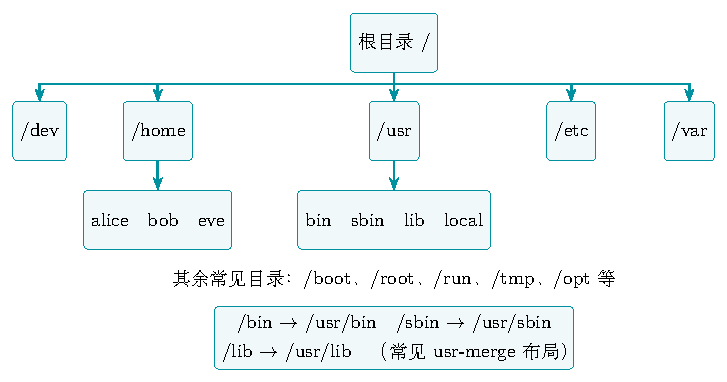
\includegraphics[width=0.9\textwidth]{linux-directory_revised.pdf}
    \caption{Linux 目录树与常见 usr-merge 符号链接} % 图片标题
    \label{fig:linux7} % 图片标签，用于引用
\end{figure}

目录树从根目录 / 出发。图中的 /home 保存用户目录，/usr 保存许多程序与库；在 Ubuntu 的 usr-merge 布局里，/bin、/sbin、/lib 通常是指向 /usr 中对应目录的符号链接，实机可用 ls -ld 检查，不只看图记结论。

\textbf{“一切皆文件”}

在linux系统中有一个非常重要的、区别于windows系统的概念是“一切皆文件”，也就是把一切资源都看作是文件，包括硬件设备（通常称为设备文件），这样好处是用户可以用读写文件的方式实现对硬件的访问。例如 U 盘连接后通常有 /dev 下的块设备节点。对原始设备节点的写入可能破坏分区数据；日常文件操作应使用挂载后的目录，不把设备节点当作普通文本文件。简单来说：你以为是 U 盘设备？其实是我文件哒！

\begin{note}
“一切皆文件”是统一接口的概括，不代表所有资源都是磁盘上的普通文件；设备、管道、套接字有不同类型和操作限制。
\end{note}

\textbf{挂载}

插入 U 盘是连接设备，挂载（Mount）则把某个文件系统接到目录树的一个挂载点上。Linux 当然也有磁盘与分区；只是访问文件时使用统一的目录路径，不按 C:、D: 这样的盘符分树。设备节点如 /dev/sdb1 用来标识分区，挂载点如 /media/alice/USB 用来访问其中的文件，二者不要混淆。

\begin{figure}[H]
    \centering
    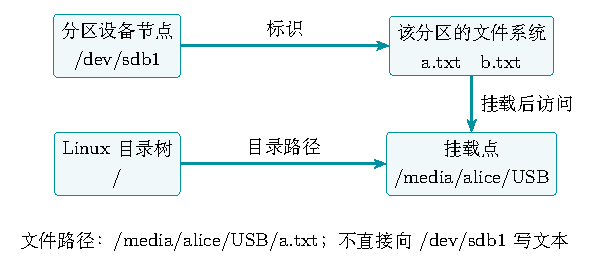
\includegraphics[width=0.85\textwidth]{mount_revised.pdf}
    \caption{把分区中的文件系统接到目录树：设备节点与挂载点各管一层} % 图片标题
    \label{fig:linux8} % 图片标签，用于引用
\end{figure}

Windows的文件系统挂载使用其内部机制完成，用户基本无法探知其过程。而Linux使用mount工具对文件系统进行挂载。挂载文件系统时，需要明确挂载点，在创建文件系统后，操作系统会提示将此文件系统挂载至哪个位置，这个位置就是挂载点，通常U盘等设备系统会自动挂载到“/media”目录下。挂载操作在备份系统镜像时经常用到。

\textbf{主要文件夹及其作用}

/bin：bin 是 Binaries (二进制文件) 的缩写, 这个目录存放着最经常使用的命令。

/boot：这里存放的是启动 Linux 时使用的一些核心文件，包括一些连接文件以及镜像文件。

/dev：dev 是 Device(设备) 的缩写, 该目录下存放的是 Linux 的外部设备，在 Linux 中访问设备的方式和访问文件的方式是相同的。

/etc：etc 是 Etcetera(等等) 的缩写,这个目录用来存放所有的系统管理所需要的配置文件和子目录。

/home：用户的主目录，在 Linux 中，每个用户都有一个自己的目录，一般该目录名是以用户的账号命名的，例如 alice、bob 和 eve。

/lib：lib 是 Library(库) 的缩写这个目录里存放着系统最基本的动态连接共享库，其作用类似于 Windows 里的 DLL 文件。几乎所有的应用程序都需要用到这些共享库。

/opt：常用于放额外安装的软件，是否为空取决于本机安装情况。

/root：该目录为系统管理员，也称作超级权限者的用户主目录。

/usr：保存许多程序、库和共享数据；不是普通用户的个人资料目录，个人文件通常放在 /home/用户名。

/var：var 是 variable(变量) 的缩写，这个目录中存放着在不断扩充着的东西，我们习惯将那些经常被修改的目录放在这个目录下。包括各种日志文件。

在这些文件夹中，绝大多数目录都包含重要的系统文件，如果随意删除可能会导致系统出错，因此在平时操作时要多加注意。

\Needspace{8\baselineskip}
\begin{example}[查看目录、设备和挂载点]


\Needspace{8\baselineskip}
\begin{tbash}
ls /
ls -ld /bin /usr/bin
ls -l /dev/null /dev/zero
findmnt /
\end{tbash}


目录类型以 d 开头，符号链接以 l 开头，字符设备以 c 开头；findmnt 显示根目录对应的文件系统。设备文件不是可随意删除的普通文件。
\end{example}
\begin{exercise}\label{ex:v1-fs-layout}
在终端执行 \texttt{ls /} 查看根目录下的文件夹，对照本节内容说出 \texttt{/etc}、\texttt{/home}、\texttt{/dev} 各自的作用；再执行 \texttt{ls /dev}，找出其中的设备文件。
\end{exercise}

\subsubsection{linux系统基本操作}
由于篇幅有限，本部分仅能列出平时操作中最常用的部分，其它内容如需用到请读者自行查阅资料。

\textbf{01用户管理}
\begin{table}[!htbp]
	\centering
	\begin{tabular}{p{0.40\textwidth}p{0.51\textwidth}}
		\toprule[1.5pt]
		命令 & 作用\\
		\midrule[1pt]
		\texttt{id   [name]}			&查看用户UID和GID信息\\
		\texttt{who}			&查看当前所有登录的用户列表\\
		\texttt{whoami}			&查看当前登录用户的账户名\\
		\texttt{su   -   [name]}			&切换用户，并且切换目录\\
		\texttt{exit}			&退出当前登录用户\\
		\texttt{passwd  [name]}			&设置用户密码\\
		\bottomrule[1.5pt]
	\end{tabular}
\end{table}

说明：
\begin{enumerate}
	\item -\enspace 可以切换到用户家目录，否则保持位置不变
	\item su 不接用户名通常尝试切换到 root；Ubuntu 默认不启用 root 密码，日常管理员命令用 sudo，不为练习开启 root 登录
	\item 命令前加sudo：以超级用户权限运行命令
\end{enumerate}

\Needspace{8\baselineskip}
\begin{example}
查看当前登录用户的账户名与 UID/GID 信息：


\Needspace{6\baselineskip}
\begin{tbash}
whoami
id
\end{tbash}


\end{example}

\begin{exercise}\label{ex:v1-user-info}
用 whoami 与 id 记录当前用户名、UID、主组和附加组，说明为什么“命令加 sudo”不等于“桌面用户永久变成 root”。
\end{exercise}
\textbf{02系统信息}

\begin{table}[!htbp]
	\centering
	\begin{tabular}{p{0.40\textwidth}p{0.51\textwidth}}
		\toprule[1.5pt]
		语法 & 作用\\
		\midrule[1pt]
		\texttt{free  [options]}			&显示系统内存使用情况\\
		\texttt{uname  [options]}			&显示电脑以及操作系统的相关信息\\
		\texttt{df  [options]  [file]}			&显示文件系统的磁盘空间使用情况\\
		\texttt{du  [options]  [directory]}			&显示目录或文件的磁盘占用量\\
		\texttt{top}			&动态显示系统中运行的进程及资源占用情况\\
		\texttt{hostname}			&查看当前主机名\\
		\bottomrule[1.5pt]
	\end{tabular}
\end{table}


\begin{table}[H]\centering
\textbf{free\enspace 选项和参数}

	\begin{tabular}{p{0.40\textwidth}p{0.51\textwidth}}
		\toprule[1.5pt]
		参数 & 作用\\
		\midrule[1pt]
		\texttt{-h}		&以易读的单位（GiB、MiB 等）显示\\
		\texttt{-m}		&以 MiB 为单位显示\\
		\texttt{-g}		&以 GiB 为单位显示\\
		\texttt{-s}\enspace [秒数] 		&每隔指定秒数持续刷新显示\\
		\bottomrule[1.5pt]
	\end{tabular}
\end{table}



\begin{table}[H]\centering
\textbf{uname\enspace 选项和参数}

	\begin{tabular}{p{0.40\textwidth}p{0.51\textwidth}}
		\toprule[1.5pt]
		参数 & 作用\\
		\midrule[1pt]
		\texttt{-a  --all}		&显示全部的信息\\
		\texttt{-m  --machine}		&显示处理器类型\\
		\texttt{-n  --nodename}		&显示主机名\\
		\texttt{-r  --release}		&显示内核版本号\\
		\texttt{-s  --sysname}		&显示操作系统名称\\
		\texttt{-v}		&显示内核构建版本信息\\
		\texttt{--help}		&显示帮助\\
		\texttt{--version}		&显示版本信息\\
		\texttt{-p}		&显示处理器信息，可能为 unknown，不保证与 -m 相同\\
		\bottomrule[1.5pt]
	\end{tabular}
\end{table}



\begin{table}[H]\centering
\textbf{df\enspace 选项和参数}

	\begin{tabular}{p{0.40\textwidth}p{0.51\textwidth}}
		\toprule[1.5pt]
		参数 & 作用\\
		\midrule[1pt]
		\texttt{-h}		&以易读的单位（GiB、MiB 等）显示\\
		\texttt{-T}		&同时显示文件系统类型\\
		\bottomrule[1.5pt]
	\end{tabular}
\end{table}



\begin{table}[H]\centering
\textbf{du\enspace 选项和参数}

	\begin{tabular}{p{0.40\textwidth}p{0.51\textwidth}}
		\toprule[1.5pt]
		参数 & 作用\\
		\midrule[1pt]
		\texttt{-h}		&以易读的单位（GiB、MiB 等）显示\\
		\texttt{-s}		&只显示总计，不列出每个子目录\\
		\texttt{--max-depth=1}		&只统计指定层级的子目录\\
		\bottomrule[1.5pt]
	\end{tabular}
\end{table}


你可以用 man 命令查阅完全的参数详情（例如\texttt{man du}查询du命令的全体参数）。

\Needspace{8\baselineskip}
\begin{example}
统计当前目录下各子目录的磁盘占用，并按易读单位显示：


\Needspace{5\baselineskip}
\begin{tbash}
du -h --max-depth=1 .
\end{tbash}


\end{example}

\Needspace{8\baselineskip}
\begin{example}[区分内存、磁盘与目录占用]


\Needspace{9\baselineskip}
\begin{tbash}
free -h
uname -r
hostname
df -hT /
du -h --max-depth=1 .
\end{tbash}


free 的 available 估计当前可用内存，df 描述根文件系统容量，du 累计当前目录文件占用。它们不是同一个“还剩多少”。
\end{example}
\begin{exercise}\label{ex:v1-disk-space}
执行 \texttt{df -hT} 查看各文件系统的磁盘使用情况，找到你的根分区（挂载点为 \texttt{/} 的一行），记录其文件系统类型、容量与已用空间；再记录 free 的 available 和 uname 的内核版本，说明这些值与磁盘容量的差别。
\end{exercise}

\textbf{03软件安装}

软件安装命令有apt，snap，yum等等，在我们ubuntu系统中用的是apt，不过有时候也得用到snap。安装和卸载软件需要root权限。

\begin{table}[!htbp]
	\centering
	\begin{tabular}{p{0.40\textwidth}p{0.51\textwidth}}
		\toprule[1.5pt]
		语法 & 作用\\
		\midrule[1pt]
		\texttt{apt  [options]   [command]   [package ...]}		&查找、安装、升级、删除软件包\\
		\bottomrule[1.5pt]
	\end{tabular}
\end{table}

\textbf{options}：可选，选项包括 -h（帮助），-y（当安装过程提示选择全部为"yes"），-q（不显示安装的过程）等等

\textbf{command}：要进行的操作

\textbf{package}：安装的包名\\


\begin{table}[H]\centering
\textbf{apt常用命令如下}

	\begin{tabular}{p{0.40\textwidth}p{0.51\textwidth}}
		\toprule[1.5pt]
		命令 & 作用\\
		\midrule[1pt]
		\texttt{apt  update}	&刷新软件包索引，不会升级已安装包\\
		\texttt{apt  upgrade}	&升级软件包\\
		\texttt{apt  list   --upgradable}		&列出可更新的软件包及版本信息\\
		\texttt{apt  full-upgrade}	&处理依赖变化的升级，可能移除包，先读变更清单\\
		\texttt{apt  install   \textless package1\textgreater   \textless package2\textgreater}	&安装指定的软件\\
		\texttt{apt  install   --only-upgrade  \textless package\textgreater}		&更新指定的软件\\
		\texttt{apt  show   \textless package\textgreater}	&显示软件包具体信息\\
		\texttt{apt  remove   \textless package\textgreater}		&删除软件包\\
		\texttt{apt  autoremove}		&清理不再使用的依赖和库文件\\
		\texttt{apt  purge \textless package\textgreater}		&移除软件包及配置文件\\
		\texttt{apt  search   \textless keyword\textgreater}		&找软件包命令\\
		\texttt{apt  list   --installed}		&列出所有已安装的包\\
		\texttt{apt  list   --all-versions}	&列出包索引中可用的各版本\\
		\bottomrule[1.5pt]
	\end{tabular}
\end{table}


与上文类似，其余命令与参数请查阅 man 手册（\texttt{man apt}）。

\Needspace{8\baselineskip}
\begin{example}
更新软件清单后安装 \texttt{tree}（一个以树状图显示目录结构的小工具）：


\Needspace{6\baselineskip}
\begin{tbash}
sudo apt update
sudo apt install tree
\end{tbash}


\end{example}

\begin{exercise}\label{ex:v1-apt-package}
使用 \texttt{apt search} 搜索并安装一个你感兴趣的小软件（如 \texttt{cowsay}），运行验证后用 \texttt{sudo apt remove} 将其卸载。
\end{exercise}

\textbf{04文件与目录管理}

先认识几个常用概念，后面的命令都要用到它们：

\begin{enumerate}
\item 绝对路径：路径的写法，由根目录\enspace /\enspace 写起，例如：/usr/share/doc 这个目录。
\item 相对路径：路径的写法，相对于当前所处的文件夹位置，不是由\enspace /\enspace 写起，例如由 /usr/share/doc 要到 /usr/share/man，可以写成：cd ../man
\item \enspace .\enspace ：表示当前目录
\item \enspace ..\enspace ：表示上一级目录
\item 文件类型：分为目录（d），文件（-），链接文件（l），装置文件里可供储存的接口设备（b），字符设备（c，例如终端、串口、/dev/null）
\item 文件基本属性：分为可读（r），可写（w），可执行（x）。Linux文件属性有两种设置方法，一种是数字，一种是符号。使用数字来代表各个权限时，各权限的分数对照为：r:4，w:2，x:1
\item 文件所有者（user）：表示该文件或目录的拥有者，也就是文件权限中的第一个权限对象（u）。
\item 用户组（group）：表示该文件或目录所属的用户组，也就是文件权限中的第二个权限对象（g）。文件权限通常依次针对文件所有者、所属用户组以及其他用户（others）进行设置。
\item 其他用户（others）：表示既不是文件所有者，也不属于该文件所属用户组的其他用户，是文件权限中的第三个权限对象（o）。
\item 路径名展开（pathname expansion）：属于 Shell（如 Bash）的语法，用于使用通配符匹配文件名。常见的通配符包括 \enspace * \enspace、\enspace ? \enspace 和 \enspace [ ] \enspace。例如：\enspace *.txt \enspace 可以匹配当前目录下所有以 .txt 结尾的文件；\enspace ? \enspace 表示匹配一个字符；\enspace [abc] \enspace 表示匹配 a、b 或 c 中的一个字符。
\end{enumerate}

处理文件和目录的命令有很多，这里分表整理了一些常用命令的语法及其选项和参数仅供大家参考


\begin{table}[H]\centering
\textbf{常用处理文件和目录的命令}

	\begin{tabular}{p{0.40\textwidth}p{0.51\textwidth}}
		\toprule[1.5pt]
		语法 & 作用\\
		\midrule[1pt]
		\texttt{ls}		&列出当前目录中的文件和子目录\\
		\texttt{pwd}		&显示当前工作目录的路径\\
		\texttt{cd  /path/to/directory}		&切换工作目录\\
		\texttt{mkdir  [directory]}		&创建新目录\\
		\texttt{cp  [source]  [destination]}		&复制文件或目录\\
		\texttt{rm  [file name]}		&删除文件或目录\\
		\texttt{mv  [old]  [new]}		&移动或重命名文件或目录\\
		\texttt{ln  [options]  [source]  [link name]}		&创建链接文件\\
		\texttt{chmod  [permissions]  [file name]}		&修改文件或目录的权限\\
		\texttt{tar  [options]  -f  archive.tar  [files...]}	&解压或压缩文件或目录\\
		\texttt{zip  [options]  output.zip  [files...]}		&压缩文件或目录\\
		\texttt{unzip  archive.zip}		&解压文件或目录\\
		\bottomrule[1.5pt]
	\end{tabular}
\end{table}



\begin{table}[H]\centering
\textbf{ls\enspace 选项和参数}

	\begin{tabular}{p{0.40\textwidth}p{0.51\textwidth}}
		\toprule[1.5pt]
		参数 & 作用\\
		\midrule[1pt]
		\texttt{-a}		&列出当前目录中全部的文件，包括隐藏文件\\
		\texttt{-d}		&仅列出目录本身，而不是列出目录内的文件数据\\
		\texttt{-l}		&长数据串列出，包含文件的属性与权限等\\
		\bottomrule[1.5pt]
	\end{tabular}
\end{table}



\begin{table}[H]\centering
\textbf{mkdir\enspace 选项和参数}

	\begin{tabular}{p{0.40\textwidth}p{0.51\textwidth}}
		\toprule[1.5pt]
		参数 & 作用\\
		\midrule[1pt]
		\texttt{-m}		&配置文件的权限\\
		\texttt{-p}		&递归创建所需目录\\
		\bottomrule[1.5pt]
	\end{tabular}
\end{table}



\begin{table}[H]\centering
\textbf{cp\enspace 选项和参数}

	\begin{tabular}{p{0.40\textwidth}p{0.51\textwidth}}
		\toprule[1.5pt]
		参数 & 作用\\
		\midrule[1pt]
		\texttt{-a}		&相当于\enspace -pdr\enspace 的意思\\
		\texttt{-d}		&若来源档为链接档的属性(link file)，则复制链接档属性而非文件本身\\
		\texttt{-f}		&强制，若目标文件已经存在且无法开启，则移除后再尝试一次\\
		\texttt{-i}		&若目标文件或目录已经存在，在覆盖时会先询问用户\\
		\texttt{-l}		&进行硬式链接的链接档创建，而非复制文件本身\\
		\texttt{-p}		&连同文件的属性一起复制过去，而非使用默认属性(备份常用)\\
		\texttt{-r}		&递归持续复制，用于目录的复制(常用)\\
		\texttt{-s}		&复制成为符号链接档，即“捷径”文件\\
		\texttt{-u}		&若 destination 比 source 旧才升级 destination\\
		\bottomrule[1.5pt]
	\end{tabular}
\end{table}



\begin{table}[H]\centering
\textbf{rm\enspace 选项和参数}

	\begin{tabular}{p{0.40\textwidth}p{0.51\textwidth}}
		\toprule[1.5pt]
		参数 & 作用\\
		\midrule[1pt]
		\texttt{-f}		&强制的意思，删除时不询问且忽略不存在的文件\\
		\texttt{-i}		&互动模式，在删除前会询问使用者是否动作\\
		\texttt{-r}		&递归删除,常用在目录的删除\\
		\bottomrule[1.5pt]
	\end{tabular}
\end{table}


\begin{note}
\texttt{rm -rf} 会不做任何确认地递归删除目标及其全部内容，且命令行下的删除不进回收站，无法恢复。这条命令删库跑路一气呵成，使用前请三思——你的存档没有读档功能。脚本中使用 \texttt{rm -rf \$dir/} 这类写法时，务必先检查变量非空：变量一旦为空，路径可能直接变成根目录。
\end{note}


\begin{table}[H]\centering
\textbf{mv\enspace 选项和参数}

	\begin{tabular}{p{0.40\textwidth}p{0.51\textwidth}}
		\toprule[1.5pt]
		参数 & 作用\\
		\midrule[1pt]
		\texttt{-f}		&强制的意思，如果目标文件已经存在，不会询问而直接覆盖\\
		\texttt{-i}		&若目标文件已经存在时，会询问是否覆盖\\
		\texttt{-u}		&若目标文件已经存在，且 source 比较新，才会升级 \\
		\bottomrule[1.5pt]
	\end{tabular}
\end{table}



\begin{table}[H]\centering
\textbf{ln\enspace 选项和参数}

	\begin{tabular}{p{0.40\textwidth}p{0.51\textwidth}}
		\toprule[1.5pt]
		参数 & 作用\\
		\midrule[1pt]
		\texttt{-s}		&创建符号链接（软链接），不加该选项时默认创建硬链接\\
		\texttt{-f}		&强制创建，若链接文件已存在则直接覆盖\\
		\bottomrule[1.5pt]
	\end{tabular}
\end{table}


\begin{conclusion}
硬链接、软链接与复制的区别：

\begin{itemize}
\item 硬链接：与源文件指向同一份数据，删除源文件不影响链接；但不能跨文件系统，也不能给目录创建；
\item 软链接（符号链接）：类似 Windows 的快捷方式，只记录源文件的路径；源文件被删除后链接失效，但可以跨文件系统、可以链接目录；
\item 复制（cp）：得到一份完全独立的新文件，与源文件互不影响。
\end{itemize}
\end{conclusion}


\begin{table}[H]\centering
\textbf{chmod\enspace 选项和参数}

	\begin{tabular}{p{0.40\textwidth}p{0.51\textwidth}}
		\toprule[1.5pt]
		参数 & 作用\\
		\midrule[1pt]
		\texttt{-R}		&进行递归的持续变更，连同次目录下的所有文件都会变更\\
		\texttt{u}		&user，用户身份\\
		\texttt{g}		&group，组 \\
		\texttt{o}		&others，其他身份 \\
		\texttt{a}		&all，全部的身份 \\
		\texttt{+  -  =}		&对权限加入，除去，设定 \\
		\bottomrule[1.5pt]
	\end{tabular}
\end{table}


使用chmod命令修改文件或目录权限有两种方式。一是用数字类型的权限属性更改，通用形式为：

chmod\enspace [-R]\enspace xyz\enspace 文件或目录

其中 xyz 是三位数字，分别对应所有者、用户组、其他用户的权限，每位数字为该身份 rwx 属性数值（r:4，w:2，x:1）的和。二是用符号类型改变文件权限，通用形式为：

chmod\enspace [身份]\enspace +/-/=\enspace [permissions]\enspace [file name]

\Needspace{8\baselineskip}
\begin{example}
先在独立练习目录创建两个空文件，再只给脚本所需权限：


\Needspace{8\baselineskip}
\begin{tbash}
touch ex1.py run.sh
chmod u+x ex1.py
chmod 755 run.sh
ls -l ex1.py run.sh
\end{tbash}


\end{example}

\begin{note}
不要图省事对所有文件都 \texttt{chmod 777}——这相当于把家门钥匙挂在门外，谁路过都能进来逛一圈。权限放得越宽，误操作和恶意篡改的风险越大；脚本只需要给所有者加上执行权限（\texttt{chmod u+x}）就够了。
\end{note}

\begin{exercise}\label{ex:v1-file-ops}
在家目录下创建 \texttt{practice} 目录，在其中新建文件 \texttt{hello.txt}，将它复制为 \texttt{hello\_bak.txt}，再把原文件移动到 \texttt{practice/sub} 目录（该目录需用 \texttt{mkdir} 一并创建），最后删除整个 \texttt{practice} 目录。
\end{exercise}


\begin{table}[H]\centering
\textbf{tar\enspace 选项和参数}

	\begin{tabular}{p{0.40\textwidth}p{0.51\textwidth}}
		\toprule[1.5pt]
		参数 & 作用\\
		\midrule[1pt]
		\texttt{-c}		&创建新的归档文件\\
		\texttt{-f}		&指定归档文件的名称\\
		\texttt{-v}		&显示详细输出，列出被添加/解压到归档中的文件 \\
		\texttt{-x}		&解压归档文件 \\
		\texttt{-z}		&使用 gzip 压缩归档文件 \\
		\texttt{-r}		&向已存在的归档中追加文件 \\
		\bottomrule[1.5pt]
	\end{tabular}
\end{table}


tar命令的参数繁多，此处只列举了以上最最常见的参数。


\begin{table}[H]\centering
\begin{note}
归档命令也有删除选项：zip 的 -m 会在压缩后移除源文件，本章练习不使用它；tar 的 -r 只适用于可追加的未压缩归档，不直接追加到 .tar.gz。先保留源数据，再做解包核验。
\end{note}
\textbf{zip\enspace 选项和参数}

	\begin{tabular}{p{0.40\textwidth}p{0.51\textwidth}}
		\toprule[1.5pt]
		参数 & 作用\\
		\midrule[1pt]
		\texttt{-r}		&递归压缩目录及其子目录中的所有文件\\
		\texttt{-e}		&为压缩文件设置密码保护\\
		\texttt{-q}		&静默模式，不显示压缩过程 \\
		\texttt{-v}		&显示详细的压缩过程 \\
		\texttt{-x}		&排除某些文件或目录，不进行压缩 \\
		\texttt{-m}		&压缩后删除原始文件 \\
		\texttt{-0}\enspace \textasciitilde\enspace \texttt{-9}		&指定压缩级别，-0 表示存储不压缩，-9 表示最高压缩率，默认是 -6 \\
		\bottomrule[1.5pt]
	\end{tabular}
\end{table}


\Needspace{8\baselineskip}
\begin{example}[硬链接、软链接和复制]
在新练习目录中执行，不改真实资料：


\Needspace{11\baselineskip}
\begin{tbash}
printf 'armor\n' > original.txt
ln original.txt hard.txt
ln -s original.txt soft.txt
cp original.txt copy.txt
printf 'radar\n' >> original.txt
ls -li original.txt hard.txt soft.txt copy.txt
cat hard.txt copy.txt
\end{tbash}


原文件与硬链接 inode 相同，内容一起变化；复制件仍只有 armor，软链接保存路径。先不删除文件，用这份状态对照前面的归纳。
\end{example}
\begin{exercise}\label{ex:v1-links-permissions-archive}
在独立目录复现链接例题，给一个练习脚本设置 755，记录 ls -l 与 ls -i。把目录打包，再解到新的空目录并比较内容。说明链接、复制、权限和归档各解决什么问题，不对设备文件 chmod 777。
\end{exercise}
\textbf{05查找、管道与重定向}


\begin{table}[H]\centering
\textbf{find\enspace 的语法}

	\begin{tabular}{p{0.40\textwidth}p{0.51\textwidth}}
		\toprule[1.5pt]
		语法 & 作用\\
		\midrule[1pt]
		\texttt{find  [path]  [option]  [expression]}		&在指定目录下查找符合条件的文件或目录\\
		\bottomrule[1.5pt]
	\end{tabular}
\end{table}


\textbf{path}：要查找的起始目录，省略时默认从当前目录开始查找

\textbf{expression}：查找条件，例如文件名、文件类型等\\


\begin{table}[H]\centering
\textbf{find\enspace 的参数}

	\begin{tabular}{p{0.40\textwidth}p{0.51\textwidth}}
		\toprule[1.5pt]
		参数 & 作用\\
		\midrule[1pt]
		\texttt{-name  pattern}		&按文件名查找，支持通配符\\
		\texttt{-iname  pattern}		&按文件名查找，忽略大小写\\
		\texttt{-type  f/d/l}		&按类型查找，f 为普通文件，d 为目录，l 为链接文件\\
		\texttt{-size  [+/-]n}		&按文件大小查找，+ 表示大于，- 表示小于\\
		\texttt{-mtime  [+/-]n}		&按修改时间查找，n 表示 n 天前\\
		\bottomrule[1.5pt]
	\end{tabular}
\end{table}


其余参数请查阅 man 手册（\texttt{man find}）。

\Needspace{8\baselineskip}
\begin{example}
先在练习目录建样本，再查找自己的文件，避免其他用户目录的权限错误干扰判断：


\Needspace{8\baselineskip}
\begin{tbash}
mkdir -p test
touch test/hello.txt
find . -type f -name "*.txt"
find . -type d -name "test"
\end{tbash}


\end{example}


\begin{table}[H]\centering
\textbf{grep\enspace 的语法}

	\begin{tabular}{p{0.40\textwidth}p{0.51\textwidth}}
		\toprule[1.5pt]
		语法 & 作用\\
		\midrule[1pt]
		\texttt{grep  [option]  pattern  [files]}		&查找文件里符合条件的字符串或正则表达式\\
		\bottomrule[1.5pt]
	\end{tabular}
\end{table}


\textbf{pattern}：表示要查找的字符串或正则表达式

\textbf{files}：要查找的文件名，可以同时查找多个文件，如果省略 files 参数，则默认从标准输入中读取数据\\

重定向是一种强大的功能，它允许用户改变命令的输入或输出方向，从而更灵活地控制数据流。重定向主要包括三种类型：标准输入重定向(stdin)、标准输出重定向（stdout）和标准错误输出重定向（stderr）。


\begin{table}[H]\centering
\textbf{重定向}

	\begin{tabular}{p{0.13\textwidth}p{0.22\textwidth}p{0.54\textwidth}}
		\toprule[1.5pt]
		输入输出 & 重定向 & 意义\\
		\midrule[1pt]
		\texttt{stdin}		& <\enspace /\enspace <<		& <从文件读取内容作为命令的输入，<<以指定字符串作为输入的结束标志\\
		\texttt{stdout}		& >\enspace /\enspace >>		& >会覆盖文件原有内容，>>则会在文件末尾追加内容\\
		\texttt{stderr}		& 2>\enspace /\enspace 2>>		&作用与标准输出重定向类似，但专门用于处理错误信息\\
		\bottomrule[1.5pt]
	\end{tabular}
\end{table}


管道符|主要用于多重命令处理，前面命令的打印结果作为后面命令的输入,不过其默认连接标准输出；失败的命令也可能有标准输出，成功的命令也可能写标准错误

管道符常和grep结合使用用于过滤信息，列出所查找关键字所在的位置


\begin{table}[H]\centering
\textbf{grep的参数}

	\begin{tabular}{p{0.40\textwidth}p{0.51\textwidth}}
		\toprule[1.5pt]
		参数 & 作用\\
		\midrule[1pt]
		\texttt{-i}		&忽略大小写进行匹配\\
		\texttt{-v}		&反向查找，只打印不匹配的行\\
		\texttt{-n}		&显示匹配行的行号\\
		\texttt{-r}		&递归查找子目录中的文件\\
		\texttt{-l}		&只打印匹配的文件名\\
		\texttt{-c}		&只打印匹配的行数\\
		\bottomrule[1.5pt]
	\end{tabular}
\end{table}


其余参数请查阅 man 手册（\texttt{man grep}）。

\Needspace{8\baselineskip}
\begin{example}
内核日志在部分机器上需要权限。先用自带样本观察 grep 的筛选与行号，再用于真实日志：


\Needspace{7\baselineskip}
\begin{tbash}
printf 'ok\nerror: sample\nok\n' > sample.log
grep -n error sample.log
cat sample.log | grep -n error
\end{tbash}


\end{example}

\Needspace{8\baselineskip}
\begin{example}[把筛选结果写入新文件]


\Needspace{8\baselineskip}
\begin{tbash}
grep -n error sample.log > errors.txt
printf 'checked\n' >> errors.txt
cat errors.txt
wc -l < errors.txt
\end{tbash}


应显示 2:error: sample 与 checked，共两行。大于号先截断目标文件，两个大于号追加，输入重定向把文件内容交给 wc；普通管道默认只传标准输出。
\end{example}
\begin{exercise}\label{ex:v1-find-python}
使用 find 在你的家目录下查找所有 7 天内修改过的 \texttt{.py} 文件。
\end{exercise}

\begin{exercise}\label{ex:v1-pipe-count}
使用管道和 grep，从 \texttt{apt list --installed} 的输出中筛选出名字包含 \texttt{python} 的软件包；再结合 \texttt{wc -l} 统计数量；将筛选结果重定向到新文件，再读取该文件统计行数并核对一致。
\end{exercise}

\textbf{06文件内容}


\begin{table}[H]\centering
\textbf{文件内容操作}

	\begin{tabular}{p{0.40\textwidth}p{0.51\textwidth}}
		\toprule[1.5pt]
		语法 & 作用\\
		\midrule[1pt]
		\texttt{cat [file name]}		&由第一行开始显示文件内容（只读）\\
		\texttt{head [file name]}		&显示文件开头的内容（默认前10行）\\
		\texttt{tail [file name]}		&显示文件末尾的内容（默认后10行）\\
		\texttt{less [file name]}		&分页查看文件内容，可上下翻页，按 q 退出\\
		\texttt{touch [file name]}		&创建空文件或更新文件的时间戳\\
		\texttt{gedit [file name]}		&创建空文件或更改文件内容\\
		\texttt{vim/vi [file name]}		&创建空文件或编辑文件内容\\
		\bottomrule[1.5pt]
	\end{tabular}
\end{table}



\begin{table}[H]\centering
\textbf{head/tail\enspace 选项和参数}

	\begin{tabular}{p{0.40\textwidth}p{0.51\textwidth}}
		\toprule[1.5pt]
		参数 & 作用\\
		\midrule[1pt]
		\texttt{-n}\enspace [行数] 		&指定显示的行数（head 与 tail 均适用）\\
		\texttt{-f}		&（仅 tail）持续跟踪文件末尾的新增内容，常用于查看日志\\
		\bottomrule[1.5pt]
	\end{tabular}
\end{table}


在所有关于文件内容的操作中，这里着重介绍一下vim。vim是从 vi 发展出来的一个文本编辑器。代码补全、编译及错误跳转等方便编程的功能特别丰富。

vi/vim 共分为三种模式，命令模式、输入模式和命令行模式

\textbf{命令模式}：用户刚刚启动 vi/vim，便进入了命令模式。此状态下敲击键盘动作会被 vim 识别为命令，而非输入字符，比如我们此时按下i，并不会输入一个字符，i被当作了一个命令。


\begin{table}[H]\centering
\textbf{命令模式常用操作}

	\begin{tabular}{p{0.40\textwidth}p{0.51\textwidth}}
		\toprule[1.5pt]
		命令 & 作用\\
		\midrule[1pt]
		\texttt{i}		&切换到输入模式，在光标当前位置开始输入文本\\
		\texttt{x}		&删除当前光标所在处的字符\\
		\texttt{:}		&切换到底线命令模式，以在最底一行输入命令\\
		\texttt{a}		&进入插入模式，在光标下一个位置开始输入文本\\
		\texttt{o}		&在当前行的下方插入一个新行，并进入插入模式\\
		\texttt{O}		&在当前行的上方插入一个新行，并进入插入模式\\
		\texttt{dd}		&剪切当前行\\
		\texttt{yy}		&复制当前行\\
		\texttt{p}		&粘贴剪贴板内容到光标下方\\
		\texttt{P}		&粘贴剪贴板内容到光标上方\\
		\texttt{u}		&撤销上一次操作\\
		\texttt{Ctrl + r}		&重做上一次撤销的操作\\
		\bottomrule[1.5pt]
	\end{tabular}
\end{table}


\textbf{输入模式}：在此状态下敲击键盘会被vim识别为输入内容，同时也有一些按键命令。


\begin{table}[H]\centering
\textbf{输入模式常用操作}

	\begin{tabular}{p{0.40\textwidth}p{0.51\textwidth}}
		\toprule[1.5pt]
		命令 & 作用\\
		\midrule[1pt]
		\texttt{keyboard+Shift}		&输入字符\\
		\texttt{ENTER}		&回车键，换行\\
		\texttt{BACK SPACE}		&退格键，删除光标前一个字符\\
		\texttt{DEL}		&删除键，删除光标后一个字符\\
		\texttt{Arrow keys}		&在文本中移动光标\\
		\texttt{HOME/END}		&移动光标到行首/行尾\\
		\texttt{Page Up/Page Down}		&上/下翻页\\
		\texttt{Insert}		&切换光标为输入/替换模式，光标将变成竖线/下划线\\
		\texttt{ESC}		&退出输入模式，切换到命令模式\\
		\bottomrule[1.5pt]
	\end{tabular}
\end{table}


\textbf{底线命令模式}：在命令模式下按下 :（英文冒号）就进入了底线命令模式。


\begin{table}[H]\centering
\textbf{底线模式基本命令}

	\begin{tabular}{p{0.40\textwidth}p{0.51\textwidth}}
		\toprule[1.5pt]
		命令 & 作用\\
		\midrule[1pt]
		\texttt{:w}		&保存文件\\
		\texttt{:q}		&退出vim编辑器\\
		\texttt{:wq}		&保存文件并退出vim编辑器\\
		\texttt{:q!}		&强制退出vim编辑器，并不保存修改\\
		\texttt{:qa!}		&不保存修改，强制退出所有打开的文件\\
		\bottomrule[1.5pt]
	\end{tabular}
\end{table}


\begin{conclusion}
Vim 启动后通常处于普通模式，按 i 进入插入模式，Esc 返回普通模式，冒号进入命令行模式。执行 :w 返回普通模式；:wq 保存并退出，:q! 放弃当前未保存修改后退出。江湖传言，"让新手自己尝试退出 vim"是一种可靠的随机字符串生成方式——卡在任何地方不知所措时，连按 \texttt{ESC} 再输入 \texttt{:q!} 即可强制退出。
\end{conclusion}

\Needspace{8\baselineskip}
\begin{example}[编辑、分页查看与退出]
运行 vim demo.txt，按 i 输入三行文字，Esc 后输入 :wq 保存退出。执行 cat demo.txt、head -n 1 demo.txt、tail -n 1 demo.txt，分别应看到全篇、第一行和末行；用 less demo.txt 查看后按 q 退出。再次进入 Vim，修改后用 :q! 退出，cat 应显示上次保存的原内容。
\end{example}
\begin{exercise}\label{ex:v1-vim-edit}
使用 vim 创建文件 \texttt{note.txt}，输入三行任意内容，保存退出后用 \texttt{cat} 验证内容；再次用 vim 打开并删除第二行，这次不保存直接强制退出，用 \texttt{cat} 确认文件没有变化。
\end{exercise}

\begin{note}
vim是一个完全可以在终端中运行的文本编辑器，功能强大，如果是远程控制等情况没有图形化界面，vim的优点就会比较突出，但是新手可能难以适应。
如果你对vim感到无从下手，可以试试更简单的终端文本编辑器nano，这个操作比较符合直觉。或者是使用在vim基础上发展的nvim，而且加入一些美化，比如AstroNvim
\url{https://astronvim.com/}（开箱即用的 Neovim 配置，安装方法见本节末尾的"AstroNvim"小节）。如果你想进行vim的命令学习，推荐vim-adventure\url{https://vim-adventures.com/}，这是一个图形化的使用vim命令的小游戏，可以轻松入门vim内容，但是完整版需要付费，也可用自带的 vimtutor 练习基础操作。
\end{note}

以上就是linux系统中关于文件和目录的基本操作，俗话说熟能生巧，请读者利用空余时间多加练习，尽快适应linux系统的命令行操作。

\subsubsection{终端里的 IDE：AstroNvim*}

Vim 本身有语法高亮与基础补全，但插件组合需要配置。Neovim（nvim）是 vim 的现代化分支，而 AstroNvim 是一套开箱即用的 Neovim 配置——装完就有文件树、模糊搜索、代码补全和漂亮的界面，毛坯房直接变精装，终端里也能有接近 IDE 的体验。

\textbf{安装新版 Neovim}

AstroNvim 需要较新版本的 Neovim（当前 AstroNvim 文档要求稳定版 0.11 及以上，安装前再次核对），而 Ubuntu 22.04 仓库自带的版本太老，因此先核对官方要求再安装。下面仅用于 \texttt{x86\_64}；ARM 机器换用对应架构包，不把主机下载包复制给 Jetson 当作同一架构。下载失败时停止，不继续解压：

\Needspace{8\baselineskip}
\begin{example}
下载并解压 Neovim 到 \texttt{/opt}，顺手装上两个依赖（ripgrep 用于全局搜索，gcc 用于编译语法高亮组件）：


\Needspace{8\baselineskip}
\begin{tbash}
curl -fLO https://github.com/neovim/neovim/releases/latest/download/nvim-linux-x86_64.tar.gz
sudo tar -C /opt -xzf nvim-linux-x86_64.tar.gz
sudo apt install ripgrep gcc
\end{tbash}


然后把刚刚解压出的 bin 目录放到 PATH 前面，这样 Shell 会优先找到新版 Neovim。下面的设置只对当前会话生效；想长期使用，可以把这一行写入自己的 Bash 或 zsh 配置，方法见第\ref{sec:shell-environment}节：


\Needspace{5\baselineskip}
\begin{tbash}
export PATH=/opt/nvim-linux-x86_64/bin:$PATH
\end{tbash}


生效后执行 \texttt{command -v nvim} 与 \texttt{nvim --version}，确认找到的是新安装的程序且版本满足要求；若旧版抢先被找到，把新目录放到 PATH 前面。
\end{example}

\textbf{安装 AstroNvim}

\Needspace{8\baselineskip}
\begin{example}
备份可能存在的旧配置，然后克隆 AstroNvim 模板并启动：

\begin{tbash}
# 目标备份名不能已存在，存在时先换名字
if [ -e ~/.config/nvim ]; then
    mv -i ~/.config/nvim ~/.config/nvim.bak
fi
if [ -e ~/.local/share/nvim ]; then
    mv -i ~/.local/share/nvim ~/.local/share/nvim.bak
fi
git clone --depth 1 https://github.com/AstroNvim/template ~/.config/nvim
nvim
\end{tbash}

\end{example}

首次启动会自动下载安装全部插件，泡杯茶等它跑完，看到编辑界面就大功告成了。条件检查会跳过不存在的旧目录；克隆或插件下载失败时先处理网络与错误，不把所有报错都忽略。

\begin{note}
保留模板的 Git 信息不妨碍本节搜索练习。已有 .bak 目录时不要覆盖，改用带日期的备份名；完整迁移还应检查 ~/.local/state/nvim 与 ~/.cache/nvim。仅在确认路径和用途后清理旧文件。
\end{note}

\begin{figure}[H]
    \centering
    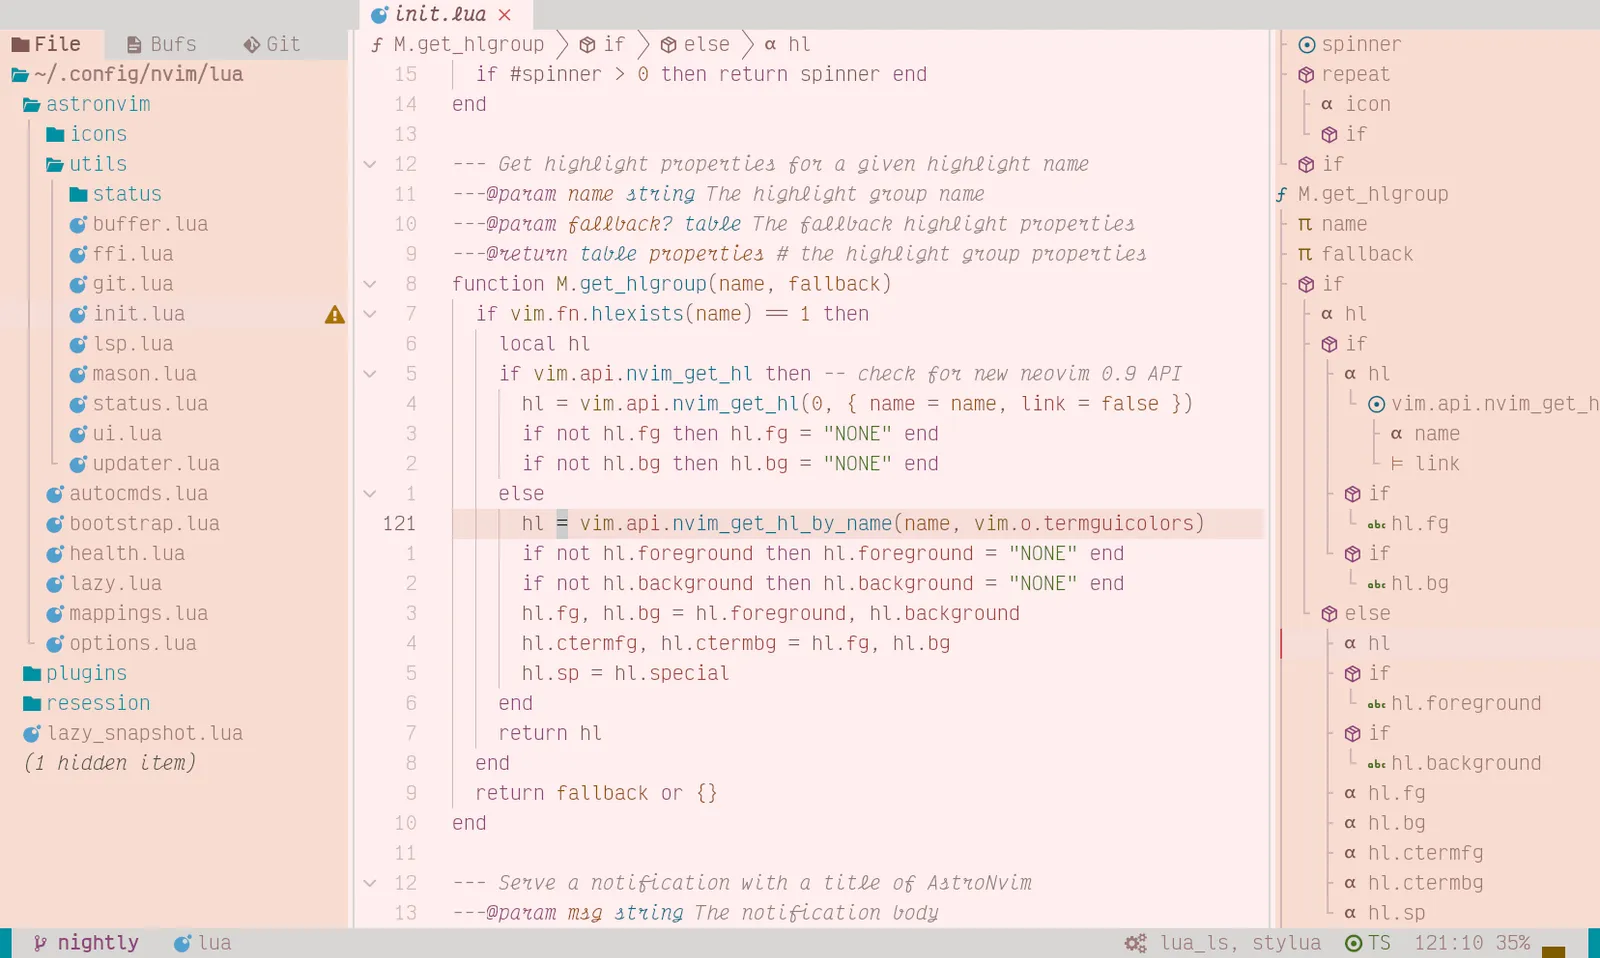
\includegraphics[width=0.8\textwidth]{astronvim_welcome.png}
    \caption{AstroNvim 界面}
    \label{fig:astronvim}
\end{figure}

\textbf{上手要点}

\begin{itemize}
\item Leader 键是空格：按下 \texttt{<Space>} 稍等片刻会弹出快捷键菜单，忘了按键组合也不用背，跟着菜单按就行；
\item \texttt{<Space>ff} 模糊搜索并打开文件，\texttt{<Space>fw} 在整个项目中搜索文字（依赖 ripgrep）；
\item 使用 \texttt{:LspInstall clangd} 安装 C++ 的语言服务器后，即可获得代码补全和跳转。
\end{itemize}

\begin{note}
界面中的图标和 zsh 的 p10k 主题一样依赖 Nerd Font，装过 MesloLGS NF 的话直接通用（见第\ref{sec:zsh-customize}节）。更多用法见官方文档：\url{https://docs.astronvim.com/}
\end{note}

\begin{exercise}\label{ex:v1-astronvim}
完成 AstroNvim 的安装，用 \texttt{<Space>ff} 打开任意一个文本文件，再用 \texttt{<Space>fw} 在某个项目目录中搜索一个关键词，体验模糊搜索。
\end{exercise}


\section{Shell 脚本与环境变量}
\subsubsection{shell简介}

在windows系统中，我们使用电脑主要是通过图形化界面点击某个图标来启动某个程序；在linux系统中我们更频繁的使用终端和命令行。然而这些都只是我们控制计算机的表象，真正能够控制计算机硬件（CPU、内存、显示器等）的只有操作系统内核（Kernel），图形界面和命令行只是架设在用户和内核之间的一座桥梁。

考虑到安全等原因，用户不能直接接触内核，因此需要另外再开发一个程序，让用户通过使用这个程序来间接地与内核进行交互。该程序的作用就是接收用户的操作（点击图标、输入命令），并进行简单的处理，然后再传递给内核。用户界面和命令行就是这个另外开发的程序，在 Linux下，这个命令行程序叫做 shell 。

\begin{figure}[H]
    \centering
    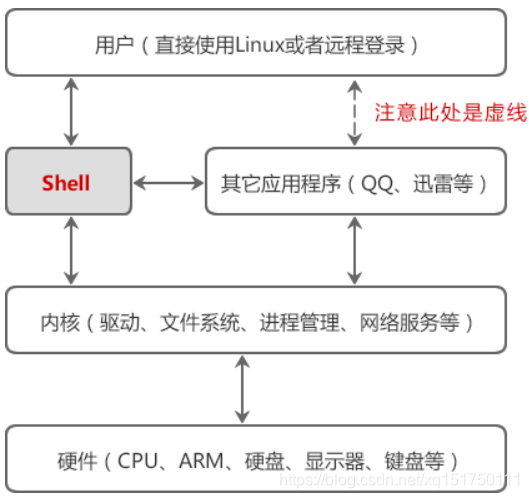
\includegraphics[width=0.7\textwidth]{shell.png}
    \caption{shell工作流程示意图} % 图片标题
    \label{fig:shell} % 图片标签，用于引用
\end{figure}

shell的一大特性就是它是一个应用程序，它连接了用户和 Linux 内核，让用户能够更加高效、安全、低成本地使用 Linux 内核。另一大特性是它是一个命令语言解释器，shell把我们在计算机上的操作或我们的命令，翻译为计算机可识别的二进制命令，传递给内核，以便调用计算机硬件执行相关的操作；计算机执行完命令后，再通过Shell翻译成自然语言，呈现在我们面前。同时，Shell 程序设计语言支持在高级语言里所能见到的绝大多数程序控制结构，比如循环，函数，变量和数组等等。

常见的shell有Bourne shell (sh), C shell (csh), Korn shell (ksh), Bourne Again shell(bash, sh 的扩展), Z shell (zsh), friendly interactive shell (fish) 等等。

启动shell的方法有两种，一是进入linux控制台，二是使用终端（快捷键为ctrl+alt+t）

\subsubsection{简单的shell脚本}

\textbf{新建一个shell脚本}

打开文本编辑器，新建一个文件 test.sh

\begin{tbash}
	vim test.sh
\end{tbash}

然后在shell脚本的第一行输入

\begin{tbash}
	#!/bin/bash
\end{tbash}

\#! 是一个约定的标记，它告诉系统这个脚本需要什么解释器来执行，即使用哪一种 shell。在第一行下面就可以用shell编程语言输入脚本内容了。

\begin{example}
一个最简单的 shell 脚本，运行后打印一行文字：
\begin{tbash}
#!/bin/bash
echo "Hello World !"
\end{tbash}
\end{example}

shell脚本可用于ROS程序自启，即编写一系列命令行操作，启动程序时无需打开终端敲命令行，只需启动一个shell脚本即可。

\textbf{运行shell脚本}

运行shell脚本也有两种方式：

\begin{enumerate}
\item 作为可执行程序

先使脚本具有执行权限

\begin{tbash}
	chmod +x ./test.sh
\end{tbash}

再执行脚本

\begin{tbash}
	./test.sh
\end{tbash}

\item 作为解释器参数

直接运行解释器，其参数就是 shell 脚本的文件名。eg:

\begin{tbash}
	/bin/sh test.sh
	/bin/php test.php
\end{tbash}

这种方式运行的脚本，不需要在第一行指定解释器信息，写了也没用
\end{enumerate}

\begin{exercise}
编写脚本 \texttt{prepare.sh}，依次执行：创建目录 \texttt{mydir}、在其中创建空文件 \texttt{a.txt}、列出 \texttt{mydir} 的内容。分别以"可执行程序"和"解释器参数"两种方式运行该脚本，并观察结果。
\end{exercise}

\subsubsection{linux中的bash}

根据刚刚对shell的介绍可以知道bash也是一种shell，事实上在大多数的linux系统中，bash是默认的缺省shell。当然如果你不想用bash也可以换成其他的shell（比如zsh也很好用）。

bash和shell一样有许多强大的功能，经常用到的有命令补全，通配符，命令历史记录，重定向，管道等等。bash的配置文件分为全局配置文件和个人配置文件：

\begin{center}
\textbf{bash主要文件}
	\begin{tabular}{cc}
		\toprule[1.5pt]
		文件 & 作用\\
		\midrule[1pt]
		$  /etc/profile    $		&系统的主配置文件，用于设置系统范围内的环境变量和其他系统的设置\\
		\texttt{\textasciitilde/.bashrc}		&用于定义用户的命令别名和本地变量\\
		\texttt{\textasciitilde/.bash\_profile}		&用于定义用户的环境变量，运行命令或脚本\\
		\bottomrule[1.5pt]
	\end{tabular}
\end{center}

其中我们会经常对.bashrc文件进行操作。

.bashrc是终端里面指令运行的配置脚本，是系统的隐藏文件，存放在\textasciitilde{} 目录下。.bashrc的功能主要有两个：

\begin{enumerate}
\item 个性化指令alias：alias [指令别名]='原指令'

注意alias和=之间不能有空格

\item 设定环境路径：export PATH=\$PATH:路径
\end{enumerate}

对.bashrc中的内容进行修改后，在下一次打开新终端时修改内容才会生效，或执行source \textasciitilde/.bashrc立刻生效。

\begin{example}
在 \texttt{.bashrc} 中添加一条别名和一个环境路径，让 \texttt{ll} 等价于 \texttt{ls -l}：
\begin{tbash}
alias ll='ls -l'
export PATH=$PATH:/opt/myapp/bin
\end{tbash}
保存后执行 \texttt{source \textasciitilde/.bashrc}，修改立即在当前终端生效。
\end{example}

\begin{exercise}
在你的 \texttt{.bashrc} 中添加别名 \texttt{cls}（等价于 \texttt{clear}），用 \texttt{source} 使其生效并验证；确认无误后将其删除，恢复原状。
\end{exercise}

\subsubsection{linux系统环境变量简介}

linux系统中有非常多的环境变量在控制系统的运行，常用的有：

\begin{enumerate}
\item PATH：决定了shell将到哪些目录中寻找命令或程序

\item HOME：当前用户主目录

\item SHELL：当前用户Shell类型
\end{enumerate}

这里我们主要介绍PATH环境变量

PATH说简单点就是一个字符串变量，当输入命令的时候linux会去查找PATH里面记录的路径，path 配置的路径下的文件可以在任何位置执行，并且可以通过which 可执行文件命令来找到该文件的位置。注意PATH是大写，linux中区分大小写。

我们先来查看一下PATH：

\begin{example}
查看当前的 PATH 环境变量：
\begin{tbash}
echo $PATH
\end{tbash}
\end{example}

终端中会输出

/usr/local/sbin:/usr/local/bin:/usr/sbin:/usr/bin:/sbin:/bin:/usr/games:

/usr/local/games:/usr/lib/wsl/lib:/snap/bin


每个路径中间用:隔开，输入命令时系统根据这些路径来寻找对应的可执行文件，先找到谁就用谁

设置环境变量的方法有两种：

\begin{enumerate}
\item export PATH=/bin:/sbin:/usr/bin:/usr/sbin

\item PATH="/bin:/sbin:/usr/bin:/usr/sbin"
\end{enumerate}

这两种方法给 PATH 赋的值完全相同，区别在于：不用 export 设置的环境变量仅对当前 shell 起作用，不会传导到子进程；export 设置的环境变量在子进程也有效，因此我们常用 export 命令来设置 PATH 环境变量。

\begin{note}
修改 PATH 时千万不要写成 \texttt{export PATH=/usr/local/mongodb/bin} 这种不带 \texttt{\$PATH} 的形式——新路径会覆盖掉所有原有路径，\texttt{ls}、\texttt{sudo} 等系统命令会集体罢工，终端里打出什么都是"找不到命令"，场面一度十分尴尬。万一写错了：终端内直接修改的，重开一个终端即可恢复；写进配置文件的，把写错的行注释掉再重开终端。
\end{note}

修改环境变量的方法有三种：

\begin{enumerate}
\item 直接在终端输入

\begin{tbash}
	export PATH=/usr/local/mongodb/bin:$PATH
\end{tbash}

\$PATH表示在原有PATH的基础上继续在前面或后面添加相应路径，这样可以避免修改原有路径。由于是在终端中输入命令，因此这种修改方式仅对当前用户当前终端有效。

\item 修改.bashrc文件：在.bashrc文件中添加export PATH=/usr/local/mongodb/bin:\$PATH一行，保存退出后source或打开新终端即可生效。该方法对当前用户永久有效。

\item 修改/etc/profile文件：找到设置PATH的行，添加export PATH=/usr/local/mongodb/bin:\$PATH，系统重启或运行source /etc/profile后生效。由于是修改了整个系统的配置文件，因此该方法对所有用户永久有效。
\end{enumerate}

\begin{conclusion}
三种修改环境变量方式的对比：

\begin{center}
\begin{tabular}{ccc}
\toprule[1.5pt]
方式 & 生效范围 & 持久性\\
\midrule[1pt]
终端中直接输入 export & 当前终端 & 关闭终端即失效\\
写入 \textasciitilde/.bashrc & 当前用户的所有终端 & 永久\\
写入 /etc/profile & 所有用户 & 永久\\
\bottomrule[1.5pt]
\end{tabular}
\end{center}

日常配置环境优先改 \textasciitilde/.bashrc：影响面小，改错了也好修。
\end{conclusion}

\begin{exercise}
在终端中直接用 export 把一个自定义目录（如 \texttt{\textasciitilde/mybin}）追加到 PATH 末尾，用 \texttt{echo \$PATH} 验证；再新开一个终端，确认该修改已失效，并说明原因。
\end{exercise}

环境变量这里介绍的很浅，主要目的是让读者先对环境变量这个概念有所了解，在后续自己配环境的过程中逐步加深对环境变量的理解，避免对系统环境变量的误操作。

\subsubsection{zsh 与终端美化*}

bash 够用，但用久了难免嫌弃：命令没有建议、语法没有高亮、提示符万年一张脸。zsh（Z shell）配合 Oh My Zsh 框架和 Powerlevel10k 主题，可以把终端武装到牙齿——命令自动建议、语法高亮、git 状态提示全都有，属于从功能机换到智能机的体验。本节为选修内容，不影响后续学习，但装完大概率就回不去了。

\textbf{安装 zsh}

\begin{example}
安装 zsh 并将它设为默认 shell：
\begin{tbash}
sudo apt install zsh
chsh -s $(which zsh)
\end{tbash}
\end{example}

\texttt{chsh} 修改的是登录 shell，需要\textbf{注销并重新登录}（或重启）后才会生效。重新登录后打开终端，会看到 zsh 的首次配置提示，按 q 跳过即可——反正接下来的配置都交给 Oh My Zsh 统一管理。

\textbf{安装 Oh My Zsh}

Oh My Zsh 是 zsh 的配置管理框架，主题和插件都通过它安装。

\begin{example}
安装 Oh My Zsh：
\begin{tbash}
sh -c "$(curl -fsSL https://raw.githubusercontent.com/ohmyzsh/ohmyzsh/master/tools/install.sh)"
\end{tbash}
\end{example}

安装脚本做的事情很简单：把框架克隆到 \textasciitilde/.oh-my-zsh 目录，并生成一份默认的 \textasciitilde/.zshrc 配置文件。

\begin{note}
如果访问 GitHub 缓慢，可以先配置代理，或使用国内镜像源安装。
\end{note}

\textbf{安装 Powerlevel10k 主题}

Powerlevel10k（简称 p10k）是目前最流行的 zsh 主题，能在提示符中直接显示目录、git 分支与提交状态、命令执行耗时等信息。

\begin{example}
安装 p10k 主题：
\begin{tbash}
git clone --depth=1 https://github.com/romkatv/powerlevel10k.git ~/.oh-my-zsh/custom/themes/powerlevel10k
\end{tbash}
然后打开 \textasciitilde/.zshrc，把主题行改为：
\begin{tbash}
ZSH_THEME="powerlevel10k/powerlevel10k"
\end{tbash}
重开终端后会自动进入 p10k 的配置向导（也可以随时用 \texttt{p10k configure} 手动启动），按提示逐项选择喜欢的样式即可。
\end{example}

% TODO(占位图)：p10k 配置向导界面截图，保存为 images/zsh_p10k_configure.png
\begin{figure}[H]
    \centering
    \IfFileExists{images/zsh_p10k_configure.png}{%
        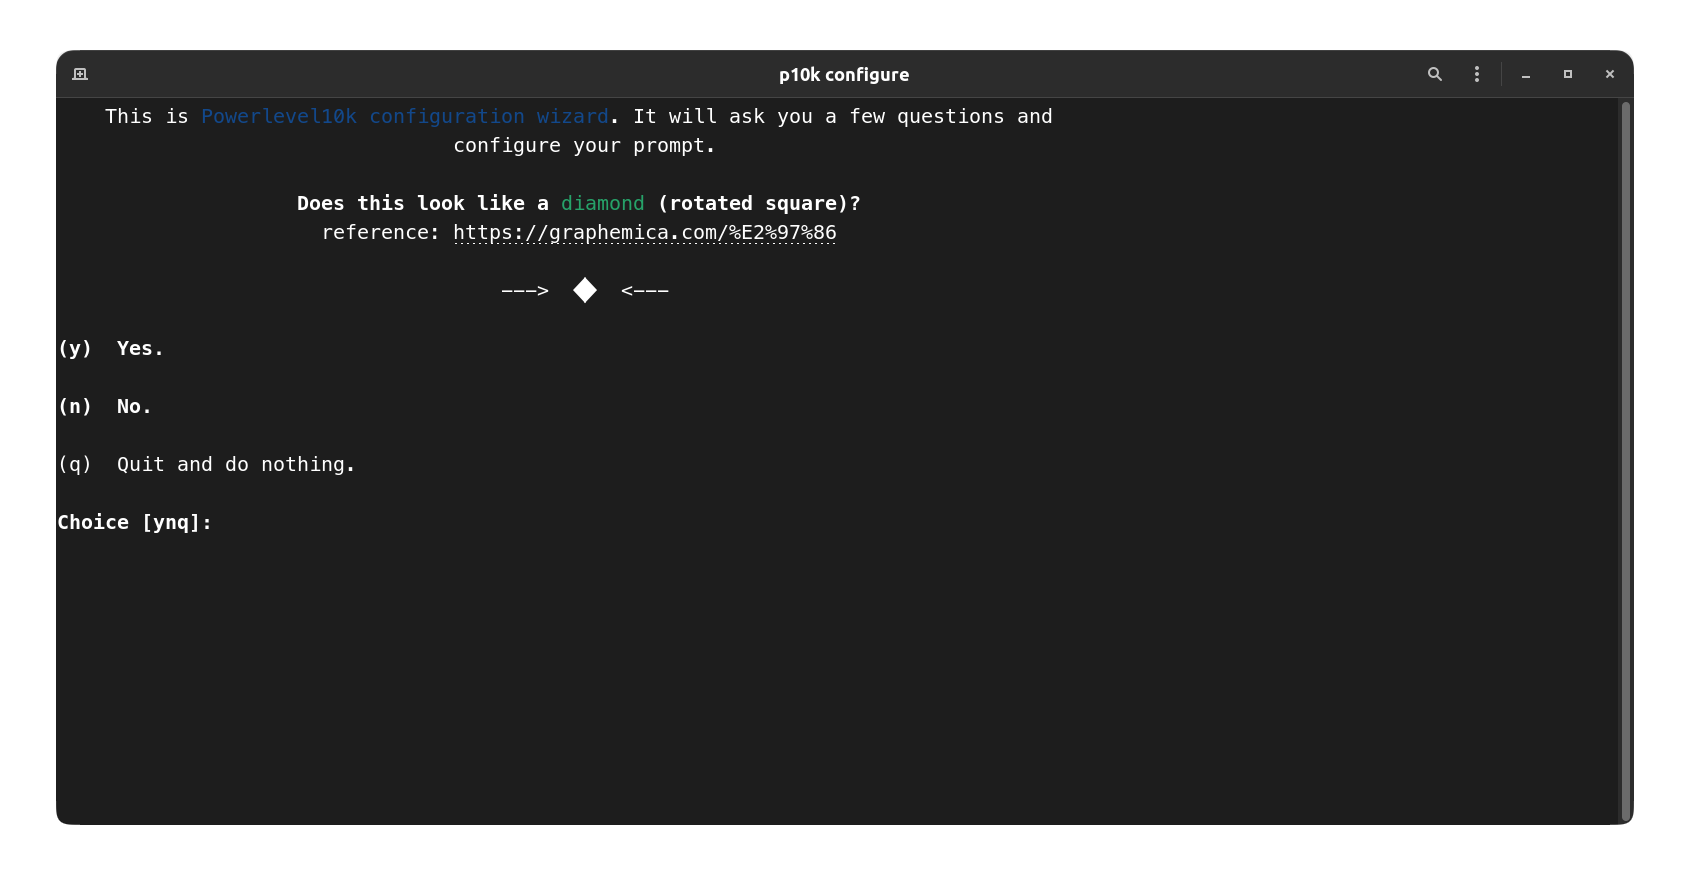
\includegraphics[width=0.8\textwidth]{zsh_p10k_configure.png}}{%
        \fbox{\parbox[c][6em][c]{0.8\textwidth}{\centering 占位图：p10k 配置向导界面（待补充截图）}}}
    \caption{p10k 配置向导}
    \label{fig:p10k_configure}
\end{figure}

\begin{note}
p10k 提示符里的图标（文件夹、git 分支符号等）依赖 Nerd Font 字体，推荐按 p10k 文档安装 MesloLGS NF，并在终端设置中把字体改为它，否则图标会显示为方块或问号。字体下载地址：\url{https://github.com/romkatv/powerlevel10k#fonts}
\end{note}

\textbf{推荐插件}

zsh 的插件生态是它相比 bash 的一大优势，最常用的两个：

\begin{itemize}
\item zsh-autosuggestions：根据历史命令给出灰色补全建议，按方向键右键采纳；
\item zsh-syntax-highlighting：命令输入时实时高亮，命令拼错时显示为红色。
\end{itemize}

\begin{example}
安装这两个插件并在 \textasciitilde/.zshrc 中启用：
\begin{tbash}
git clone https://github.com/zsh-users/zsh-autosuggestions ~/.oh-my-zsh/custom/plugins/zsh-autosuggestions
git clone https://github.com/zsh-users/zsh-syntax-highlighting ~/.oh-my-zsh/custom/plugins/zsh-syntax-highlighting
\end{tbash}
然后修改 \textasciitilde/.zshrc 中的插件行：
\begin{tbash}
plugins=(git zsh-autosuggestions zsh-syntax-highlighting)
\end{tbash}
\end{example}

% TODO(占位图)：配置完成的终端效果图（含 p10k 提示符、自动建议、语法高亮），保存为 images/zsh_p10k_effect.png
\begin{figure}[H]
    \centering
    \IfFileExists{images/zsh_p10k_effect.png}{%
        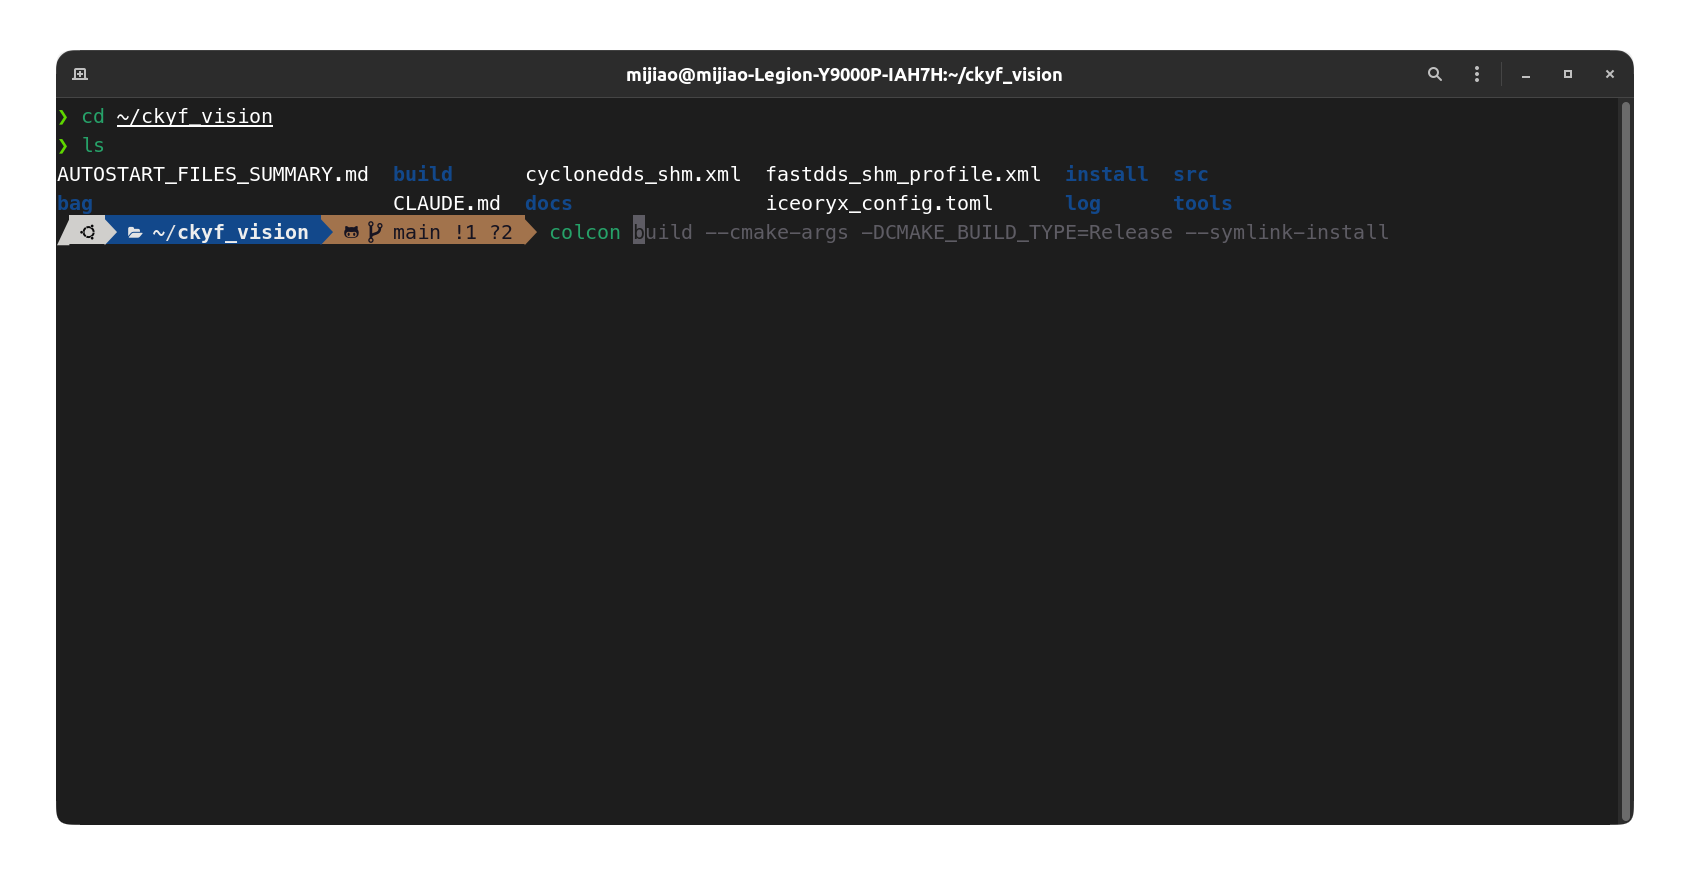
\includegraphics[width=0.8\textwidth]{zsh_p10k_effect.png}}{%
        \fbox{\parbox[c][6em][c]{0.8\textwidth}{\centering 占位图：美化后的终端效果（待补充截图）}}}
    \caption{配置完成后的终端效果}
    \label{fig:zsh_effect}
\end{figure}

\textbf{与 bash 的不同}

换用 zsh 后，日常使用的大部分命令完全一样，但有一些区别需要知道：

\begin{conclusion}
zsh 与 bash 的主要区别：

\begin{center}
\begin{tabular}{ccc}
\toprule[1.5pt]
对比项 & bash & zsh\\
\midrule[1pt]
配置文件 & \textasciitilde/.bashrc & \textasciitilde/.zshrc\\
通配符无匹配时 & 原样保留（如 \texttt{*.txt}） & 报错 no matches found\\
数组下标 & 从 0 开始 & 从 1 开始\\
Tab 补全 & 基础补全 & 支持命令参数、选项的智能补全\\
\bottomrule[1.5pt]
\end{tabular}
\end{center}

两者脚本语法大部分兼容；带 \texttt{\#!/bin/bash} 行首的脚本仍由 bash 执行，更换交互式 shell 不影响已有脚本的运行。
\end{conclusion}

\begin{note}
\textasciitilde/.bashrc 中的内容不会自动迁移到 \textasciitilde/.zshrc——尤其是 source 类的环境配置行（后续卷二安装 ROS2 时会向 \textasciitilde/.bashrc 写入 source 命令）。换用 zsh 后记得手动把这些行加到 \textasciitilde/.zshrc 里，否则会出现"昨天还能编译，今天找不到命令"的灵异事件。
\end{note}

\begin{exercise}
完成 zsh、Oh My Zsh、p10k 的安装与主题配置，启用 autosuggestions 插件，并把原来 \textasciitilde/.bashrc 中自己添加的别名迁移到 \textasciitilde/.zshrc。
\end{exercise}



\section{Git 工具的使用}
\subsubsection{Git 管什么，GitHub 又是什么}
代码昨天还能跑，今天改了几处却坏了，这时候如果只有一个“最终版.cpp”，就不太容易找回昨天的状态了。我们需要版本控制（Version Control），把每次有意义的改动记录下来，之后既能查看改过什么，也能找回已经提交的内容。Git 就是这样的工具，它在本地保存提交（Commit）和历史，也能帮助多人协作。

这里先分清 Git 和 GitHub：Git 是我们使用的版本控制工具，GitHub 是可以托管 Git 仓库的网站之一，装了 Git 并不等于注册了 GitHub。Git 也可以完全离线使用，所以我们先在练习目录里学操作，把流程走通，再去处理比赛工程。
\Needspace{8\baselineskip}
\begin{example}[检查工具]
Ubuntu 可先运行 \texttt{git --version}；命令不存在时用 \texttt{sudo apt install git} 安装。成功应打印版本，装工具不等于创建仓库。后面的本地实验需要 Git 2.28 或以上。
\end{example}

\subsubsection{四个区域与提交身份}
\label{sec:git-regions}
Git 的名字一下子有点多，我们先让四个区域混个脸熟，不用急着背，后面的实验都会用到。工作区（Working tree）就是你正在编辑的文件；暂存区（Index）保存这次准备提交的版本；本地仓库记录已经提交的历史；远程仓库则是另一份用来交换提交的仓库，通常在服务器上，也可以像下面的实验一样放在本机。
\begin{figure}[H]
\centering
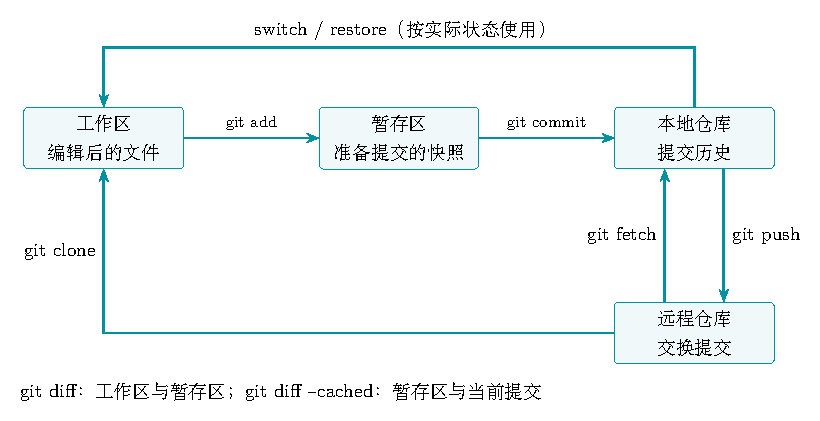
\includegraphics[width=0.9\textwidth]{git-workflow_revised.pdf}
\caption{Git 四个区域：箭头上的命令说明内容在哪两处之间流转}
\label{fig:git}
\end{figure}
顺着图里的箭头看，我们编辑好文件后，用 \texttt{git add 路径} 把当前版本放到暂存区。这里保存的是 add 时的版本，如果随后又改了同一个文件，还要重新 add。接下来用 \texttt{git commit -m '说明'} 把暂存内容记成一次本地提交，再用 \texttt{git push 远程 分支} 发给远程仓库，队友才能从那里获取。

如果不知道自己走到了哪一步，可以先看 \texttt{git status}。想看具体改动，\texttt{git diff} 比较工作区和暂存区，\texttt{git diff --cached} 比较暂存区和当前提交。这两个 diff 看的是不同位置，后面我们会用同一个文件对比一次。

\Needspace{8\baselineskip}
\begin{example}[只配置练习仓库的作者]
在新目录操作，名称可换成自己的：


\Needspace{11\baselineskip}
\begin{tbash}
mkdir git-config-lab
cd git-config-lab
git init --initial-branch=main
git config user.name 'Training Student'
git config user.email 'student@example.invalid'
git config --local --get user.name
git config --local --get user.email
\end{tbash}


执行后应该能读回刚设置的名字和邮箱。\texttt{git config [作用域] 键 值} 用来设置配置，\texttt{--get} 则读取它；这里不加全局作用域，只改当前练习仓库。如果以后想让自己的仓库通常都使用同一份身份，可以加 \texttt{--global} 设置当前用户的通用配置。还有一点别弄混：名字和邮箱是提交里的作者信息，不是 GitHub 登录认证，填了邮箱也不会自动获得推送权限。
\end{example}
\begin{exercise}\label{ex:v1-git-config}
新建独立仓库，设置并读回本地作者身份。解释 add 后再改文件为何可以同时出现“已暂存”和“未暂存”状态；通过一次实际修改核对。
\end{exercise}

\subsubsection{从修改到远程：不联网的完整实验}
\label{sec:git-local-demo}
概念看过了，我们来完整走一遍。项目放在本卷 \texttt{examples/git-workflow-demo/}，只有 \texttt{demo.sh} 和 \texttt{README.md}。这一次把“远程”也放在本地临时目录里，你不用先处理网站账号和网络认证，就能看清文件是怎样从自己的工作区走到队友那里去的。
\Needspace{8\baselineskip}
\begin{example}[两次提交与另一份克隆]
目录中唯一的核心脚本完整如下：

\lstinputlisting[language=bash,frame=single,numbers=left,breaklines=true]{examples/git-workflow-demo/demo.sh}

从本卷目录运行：


\Needspace{6\baselineskip}
\begin{tbash}
cd examples/git-workflow-demo
bash demo.sh
\end{tbash}


\texttt{git init --bare} 建立不含普通工作区的“远程”；\texttt{git clone 仓库 目录} 获取一份本地工作副本。脚本第一次写 camera 后 add、commit、push；第二次写 radar，先看工作区差异，再 add 看暂存差异，最后提交并推送。\texttt{-u} 记录上游，此后在同一分支可直接 push。

运行时先看看 WORKTREE DIFF，再看看 STAGED DIFF：里面都有新增的 radar，但它们出现在 add 前后两个阶段。最后 TEAMMATE CONTENT 应该是 camera、radar 两行，COMMIT COUNT 为 2。我们在 teammate 这份克隆里看到了两次提交，就说明它们确实已经进入远程，不只是留在 student 的本地仓库里。第一次克隆时提示空仓库，是因为我们刚刚创建的“远程”还没有内容；后面如果还有失败提示，就要按具体错误处理，不能都当成这条警告忽略掉。
\end{example}
\begin{exercise}\label{ex:v1-git-commits}
在脚本打印的 student 仓库中增加第三行并提交，先\textbf{不推送}。记录 student 和 remote 的提交数，再 push，最后在 teammate 中执行 \texttt{git pull --ff-only} 并检查第三行。解释为什么本地 commit 成功不代表队友已经收到。
\end{exercise}

\subsubsection{分支、合并与实际远程}
如果你正在写新功能，又不想把没写完的东西直接混进主线，我们就可以开一个分支（Branch）。它是指向某次提交的可移动名字，不是把整个项目永久复制一遍。等功能写完、差异也检查过了，再合并（Merge）回主线。分支 A 和分支 B 表示：我们联合！不过联合之前，还是先看清各自改了什么。
\Needspace{8\baselineskip}
\begin{example}[没有冲突的最小分支实验]
在刚才的 student 仓库中执行；开始前 \texttt{git status --short} 应为空，不能把未完成修改顺手混入实验：


\Needspace{11\baselineskip}
\begin{tbash}
git switch -c feature-note
printf 'check timestamps\n' > review.txt
git add review.txt
git commit -m 'Add review note'
git switch main
git merge --ff-only feature-note
git log --oneline --graph -4
\end{tbash}


执行完再看 main，应该已经出现了新文件，日志里也能找到刚刚的提交。因为 main 没有另外前进，它可以直接沿着这条历史走到新位置，这就叫快进。\texttt{--ff-only} 只允许这种情况；如果两条分支各自有了新提交，它会拒绝，而不是自动帮我们解决冲突。你在旧教程里看到的 \texttt{checkout -b 名称} 也能创建并切换分支，这里我们使用职责更明确的 switch。
\end{example}
\begin{exercise}\label{ex:v1-git-branch}
在自己的练习仓库创建另一个分支，增加一个小文件并提交，切回 main，合并并查看图形日志。指出分支名、提交与工作文件的关系，最后保留记录，不操作真实远程。
\end{exercise}

换成服务器仓库时，\texttt{git remote -v} 查看地址，\texttt{git fetch 远程} 取回提交但不合并工作区，\texttt{git pull} 包含取回及整合步骤，\texttt{git push} 把本地分支的提交发出去。HTTPS 的访问令牌与 SSH 密钥是认证方式，按托管服务说明设置，不在教材、脚本或提交中写凭据。已有上游时使用简短命令；无上游时先核对远程名和当前分支，不假设都叫 origin/main。
\begin{note}
\texttt{git reset --hard} 会丢弃所覆盖路径的未提交修改；强制推送会改写远程历史，影响队友。本章不需要这些操作。合并冲突时先读 status 和冲突块，确认两边意图，编辑后 add、commit；想取消未完成合并，可先保存新增工作，再按实际状态使用 \texttt{git merge --abort}。未提交内容没有可靠的 Git 恢复保证。
\end{note}

\subsubsection{忽略构建产物}
工程编译几次后，目录里通常会多出构建产物和日志，我们不必把它们每次都交给队友。可以用 \texttt{.gitignore} 告诉 Git，哪些未跟踪文件可以忽略。不过已经跟踪过的文件，不会因为写进了这份名单就自动退出历史。

常用的模式有 \texttt{*.log}（匹配日志）、\texttt{/build/}（仓库根目录下的 build）和 \texttt{!路径}（取消忽略）。如果想忽略 build 里的大部分文件，又保留一个例外，就要留意：把父目录整个忽略以后，Git 不会再进去寻找例外。下面我们实际试一下。
\Needspace{8\baselineskip}
\begin{example}[保留 build 中的一个文件]
在练习仓库创建 \texttt{.gitignore}：
\begin{lstlisting}[language={},frame=single]
*.log
/build/*
!/build/keep.txt
\end{lstlisting}
然后验证：


\Needspace{8\baselineskip}
\begin{tbash}
mkdir -p build
touch run.log build/cache.tmp build/keep.txt
git status --short --untracked-files=all
git check-ignore -v run.log build/cache.tmp
\end{tbash}


status 应列出 .gitignore 与 build/keep.txt，不显示另两项。已跟踪文件若确实要停止跟踪，可用 \texttt{git rm --cached 路径} 后提交；这保留工作文件，\textbf{不会抹去旧提交里的内容或泄露过的凭据}。
\end{example}
\begin{exercise}\label{ex:v1-git-ignore}
为自己新建的日志与构建目录设置上述忽略与例外规则，实际核对 status。解释先写 /build/ 再取消忽略 keep.txt 为何通常不能达到目标。
\end{exercise}
\begin{conclusion}
Git 操作先问“我正在改哪个区域”：编辑改工作区，add 更新暂存快照，commit 建本地历史，push 交换提交。分支组织历史，忽略规则控制未跟踪文件。每次提交前看 status、diff 和 diff --cached，避免把旧产物或无关文件一起交给队友。
\end{conclusion}
官方命令与忽略规则可在 \url{https://git-scm.com/docs} 查；想观察分支关系可用 \href{https://learngitbranching.js.org/?locale=zh_CN}{Learn Git Branching 中文版}，网页动画辅助理解，不能代替本地文件验证。


\section{Conda 的简单使用*}
\subsubsection{先判断是否需要 Conda}
一个 Python 项目要求这个版本的包，另一个项目又要求那个版本，如果都装进同一套环境里，很容易互相打架。这时候我们可以用环境管理器（Environment Manager），给每个项目准备一套相对独立的解释器和依赖，用哪个项目就切到哪套环境，不必每次都拆东墙补西墙。

Conda 就是同时管理解释器、包和环境的工具。如果你接触的 Python 项目不多，只需要系统 Python 和几个包，也可以跳过 Conda，用标准库自带的 venv，更轻量一些。
\begin{note}
环境隔离不是安全沙箱，也不保证所有依赖冲突都消失。安装器与下载渠道按当前官方说明核对：\url{https://docs.conda.io/projects/conda/en/stable/user-guide/install/}。已装好就不重复安装；\texttt{conda --version} 应能显示版本，\texttt{conda info --base} 能找到安装位置。
\end{note}

\subsubsection{先读配置，再决定是否更改}
安装好以后，我们先看看它现在怎样工作，不急着把网上的配置整段复制进去。Conda 可以从用户的 \texttt{\textasciitilde/.condarc} 等位置读取配置，\path|conda config --show-sources| 告诉你配置来自哪里，\texttt{--show 键名} 显示实际值，\texttt{--set 键名 值} 则用来设置单值。

下载慢时可以按当前渠道文档选择镜像，不过混用渠道可能影响依赖解算和许可适用条件，要按项目需要核对，不能把“加得越多就越容易装好”当成经验。
\Needspace{8\baselineskip}
\begin{example}[检查自动激活与下载渠道]


\Needspace{8\baselineskip}
\begin{tbash}
conda config --show-sources
conda config --show channels
conda config --show auto_activate_base
conda env list
\end{tbash}


先记下实际的渠道和环境列表。如果每次打开终端都会自动进入 base，而你并不总要用它，可以关闭基础环境的自动激活。已有 .condarc 时先备份自己的文件，然后执行：


\Needspace{5\baselineskip}
\begin{tbash}
conda config --set auto_activate_base false
\end{tbash}


接着从平时的入口新开一个终端，看看是不是不再自动进入 base。后面学习 ROS 2 时，Conda 的 PATH 或库路径可能干扰系统工具链，所以养成按需激活的习惯会更省心。如果你的版本提示键名或别名有变化，就用 \texttt{conda config --describe} 查当前支持项，不用猜一个名字反复改。
\end{example}
\begin{exercise}\label{ex:v1-conda-config}
只读记录配置来源、下载渠道与基础环境自动激活状态。说明哪些值来自用户配置、哪些来自默认值，以及为什么后续 ROS 2 编译前要确认没有继承 Conda 的 PATH/库路径。没有 Conda 时先使用 venv 的独立环境路线，Conda 命令检查留待安装后验证。
\end{exercise}

\subsubsection{创建、使用与删除练习环境}
配置看过了，我们来给一个小项目准备环境。创建时使用 \texttt{conda create --name 名称 python=版本 [包名]}，其中名称和版本按你的项目需要填写；创建好后，用 \texttt{conda activate 名称} 进入，\texttt{conda install 包名} 安装依赖，不用了再用 \texttt{conda deactivate} 退出。激活改变的是当前 Shell 使用的命令与依赖，旁边已经打开的其他终端不会自动跟着切换。
\Needspace{8\baselineskip}
\begin{example}[只给一个练习环境装 NumPy]
先在 \texttt{conda env list} 确认没有同名资料，再执行：


\Needspace{11\baselineskip}
\begin{tbash}
conda create --name rm-training-py310 python=3.10
conda activate rm-training-py310
conda install numpy
python --version
python -c "import sys, numpy; print(sys.executable); print(numpy.__version__)"
conda list numpy
conda deactivate
\end{tbash}


这时候应该显示 Python 3.10，解释器路径也应当落在刚创建的环境里，并且能够成功导入 NumPy。别只看提示符前面多了一个环境名，就认定切换完成了；我们再看一次实际路径、试一次导入，才能确认这条 python 命令真的用上了它。
\end{example}
\begin{note}
\texttt{conda remove --name 名称 --all} 会删除指定环境的全部包。先退出并核对名称；不要把平时使用的环境拿来练删除。环境解决软件依赖，ROS 2 的 Bash/zsh 加载脚本另按卷二说明，不把它们写入所有 Shell 的通用启动流程。
\end{note}
\begin{exercise}\label{ex:v1-conda-env}
独立完成 Python 3.10 与 NumPy 环境的创建、激活、导入验证和退出，记录解释器路径。确认环境只用于练习后删除，再检查环境列表与当前 Python 路径。保留日志，失败时记录下载或解算错误，不宣称“提示符变了就是成功”。
\end{exercise}
\begin{conclusion}
配置决定渠道与激活行为，环境决定这次项目用哪套解释器和包。先读实际值，再改用户范围；先验证路径与导入，再清理练习环境。ROS 2 工作空间使用其支持的系统环境，深度学习项目的 Conda 环境按需单独激活。
\end{conclusion}


\section{本章小结}
本章围绕"装好系统 → 用好系统 → 护好系统"这条主线展开：

\begin{itemize}
\item \textbf{安装与维护}：双系统安装的四个流程（分区、制作启动盘、安装、设置）需要亲手走一遍；timeshift 快照相当于配环境前的存档位，每次大改环境前都应先存档，环境炸了随时回档。系统扩容、grub 美化、卸载重装属于选修内容，用到时再回来查即可。
\item \textbf{命令行基础}：目录结构、"一切皆文件"与挂载是必须理解的概念；文件管理（ls/cp/mv/rm）、查找（find/grep）、重定向与管道、vim 基本操作是每天都要用的基本功，要求熟练；各命令的参数不必死记，会用参数表和 man 手册查即可。
\item \textbf{shell 与环境变量}：会编写并运行简单的 shell 脚本；理解 PATH 的作用，掌握修改环境变量的三种方式及其生效范围，日常配置优先写入 \textasciitilde/.bashrc。
\item \textbf{git}：理解工作区、暂存区、本地版本库、远程仓库四个区域的流转关系，熟练掌握 add/commit/push/pull 的日常闭环，会写基本的 .gitignore。
\item \textbf{conda}（选修）：会创建、激活、退出和删除虚拟环境，配环境时先在虚拟环境中试错。
\end{itemize}

完成本章验收后，就可以揣着新装好的系统进入第 2 章了。配置环境的道路还会不断延伸——不要停下来啊，第 2 章现代 C++ 见。

\begin{problemset}
\item 说出双系统安装的四个主要流程，并解释安装类型为什么必须选择"其它选项"。
\item 解释"挂载"的含义，并说明 U 盘插入 Ubuntu 后一般被自动挂载到哪个目录下。
\item 写出命令：以易读单位统计当前目录下各子目录的磁盘占用（只统计一层）。
\item 解释 \texttt{chmod 755 run.sh} 中三个数字各自的含义，并写出与之等价的符号写法。
\item 写出命令：在 \texttt{/etc} 目录下查找所有以 \texttt{.conf} 结尾的文件，并把结果保存到家目录下的 \texttt{conf\_list.txt} 中。
\item 说明 \texttt{./test.sh} 与 \texttt{bash test.sh} 两种脚本运行方式的区别，以及前者为什么需要先执行 \texttt{chmod +x}。
\item 说明 git 中工作区、暂存区、本地版本库三者的区别，以及 \texttt{git add} 与 \texttt{git commit} 各自的作用。
\item （提高）比较 timeshift 快照与 tar 系统镜像两种备份方式，说明各自适用的场景。
\item （提高）若把 PATH 误写为 \texttt{export PATH=/opt/app/bin}（未包含原来的 \texttt{\$PATH}），会出现什么现象？分别就"终端内直接修改"和"写入 .bashrc"两种情况说明恢复方法。
\item （实践）编写脚本 \texttt{backup.sh}：将家目录下指定的某个目录打包为以当天日期命名的 \texttt{tar.gz} 文件，保存到 \texttt{\textasciitilde/backups} 目录中，并解压验证内容完整。
\end{problemset}

% ============================================================
\chapter{现代 C++ 基础}

\begin{introduction}
  \item 学习目标：掌握类、继承与模板；编写 lambda；理解引用与移动；使用智能指针与常用 STL；掌握多线程同步与常见模型，并理解进程内存分区与堆栈差异。
  \item 建议学时：约 1.5--2 周。
  \item 本卷边界：ROS2 执行器与节点生命周期中的多线程用法见卷二；本节只讲标准 C++ 并发工具、经典问题与基础线程池。
\end{introduction}

\section{面向对象编程：类}
\subsubsection{类的基本概念}

类是\textbf{面向对象}（OO，Object-Oriented）最基本的概念，也是C++区别于C语言的重要特征。
面向对象编程的基本思想是抽象出对象，将对象作为程序的基本单元，通过消息传递来进行通信和协作。
对象是类的实例，具有状态和行为：状态存储在对象的数据成员中，行为由对象的成员函数实现。
面向对象编程的优点是代码的可重用性、可扩展性和可维护性都得到了提高。

在C++中，类是一种抽象数据类型，它定义了对象的行为和状态，并提供了对这些数据的访问接口。
类可以包含数据成员、成员函数、构造函数、析构函数等，其中能从外部访问的成员构成了类的接口，私有成员则留给类自己管理。
类可以派生出新的类，从而实现代码的重用和扩展。

类的语法看起来零碎，我们先用小程序把成员声明、创建对象和调用连起来。项目放在 \path{examples/class-basics-demo}，文件组成如下。每个 cpp 都有自己的 main，分别编译；不要把它们拼成一个文件。
\begin{lstlisting}[language={}]
class-basics-demo/
  README.md
  class-template.cpp
  constant-template.cpp
  constructors.cpp
  designated.cpp
  function-template.cpp
  inheritance.cpp
  operators.cpp
  overload.cpp
  skeleton.cpp
  static-friend.cpp
\end{lstlisting}
编译命令里，-std 指定 C++ 标准，-Wall/-Wextra 打开常用警告，-pthread 配置线程编译与链接；-o 指定临时输出文件。先进入项目目录，后面的源码名按当前示例替换。

\Needspace{9\baselineskip}
\begin{example}
类的基本结构（先认识成员，再创建对象调用）：
\lstinputlisting[language=C++,numbers=left,numberstyle={\color{gray}\tiny}]{examples/class-basics-demo/skeleton.cpp}

从本卷目录进入 \path{examples/class-basics-demo}，保存的源码就是 \texttt{skeleton.cpp}。
\begin{tbash}
g++ -std=c++17 -Wall -Wextra -pthread skeleton.cpp -o /tmp/cpp-demo
/tmp/cpp-demo
\end{tbash}
这里输出 1，说明对象已经构造，公有成员函数可以使用私有数据。
\end{example}

\begin{enumerate}
    \item \textbf{构造函数和析构函数}：负责对象的初始化和释放，构造函数与类同名，析构函数在类名前加 \texttt{\textasciitilde}，两者都不写返回类型。
    \item \textbf{成员函数}：实现类的行为，它们实现了类的功能。
    \item \textbf{数据成员}：存储类的数据信息。
\end{enumerate}

\begin{center}
    \begin{tabular}{cc}
        \toprule[1.5pt]
        修饰限定符 & 作用 \\
        \midrule[1pt]
        private & 该类的成员和友元可以访问 \\
        public & 可以被类外的其他函数或派生类中函数调用 \\
        protected & 该类的成员、友元与派生类按规则访问 \\
        \bottomrule[1.5pt]
    \end{tabular}
\end{center}

顺带一提，C++是一门\textbf{多范式}语言：既可以像C语言那样面向过程（数据和函数分离，通过函数调用组织逻辑），
也可以面向对象，还可以用模板进行泛型编程。本章后面的小节会逐一见到它们。

\begin{note}
\texttt{struct} 和 \texttt{class} 在 C++ 中几乎完全等价，\textbf{唯一的区别是默认权限}：
\texttt{struct} 的成员默认 \texttt{public}、默认公有继承；\texttt{class} 的成员默认 \texttt{private}、默认私有继承。
除此之外，\texttt{struct} 一样可以有构造函数、成员函数、继承和多态。
习惯上 \texttt{struct} 用于纯数据打包（如坐标点），\texttt{class} 用于需要封装的对象。
\end{note}

\textbf{番外：指名初始化（Designated Initializers）。}
对于下面这种成员公开、没有用户声明构造函数的简单结构体（聚合类型，Aggregate Type），C++20 允许在初始化时指名道姓地给成员赋值。
不过成员名仍要按声明顺序写，不能因为写了名字就随意调换；这里先认识最简单的用法：

\Needspace{9\baselineskip}
\begin{example}
指名初始化：
\lstinputlisting[language=C++,numbers=left,numberstyle={\color{gray}\tiny}]{examples/class-basics-demo/designated.cpp}


从本卷目录进入 \path{examples/class-basics-demo}，保存的源码就是 \texttt{designated.cpp}。
\begin{tbash}
g++ -std=c++20 -Wall -Wextra -pthread designated.cpp -o /tmp/cpp-demo
/tmp/cpp-demo
\end{tbash}
这里输出 1 3。把 .a、.b 的顺序调换后，C++20 编译应失败，名字不能替代顺序规则。
\end{example}

\begin{exercise}\label{ex:v1-cpp-point}

定义一个 \texttt{Point} 类，包含私有数据成员 \texttt{x}、\texttt{y}（\texttt{double} 类型），
编写含参构造函数和打印坐标的成员函数，并在 \texttt{main} 中创建两个点验证。
\end{exercise}

\subsubsection{静态和友元}

\textbf{静态成员}（static member）属于整个类，而不是某个具体对象。
无论创建多少个对象，静态成员在内存中只有一份，被类的所有对象共享，因此可以实现一些全局变量的功能。
普通静态数据成员在类内用 \texttt{static} 关键字\textbf{声明}，用到时在类外提供一次\textbf{定义}。
从 C++17 起，也可以写成 \texttt{inline static int count = 0;}，直接在类内定义。静态成员函数没有 \texttt{this}，不能直接访问某个对象的非静态成员。
这里的静态数据成员具有静态存储期，不会随着某一个对象的析构一起消失。

\textbf{友元函数}（friend function）：有时我们希望某个函数可以访问类的私有成员，但又不希望它成为类的成员函数。
这时可以在类的声明中用 \texttt{friend} 关键字把它声明为友元函数。友元函数不是类的成员，实现时不加类的作用域，
但可以访问类的私有成员。

\Needspace{9\baselineskip}
\begin{example}
静态成员与友元函数的用法：
\lstinputlisting[language=C++,numbers=left,numberstyle={\color{gray}\tiny}]{examples/class-basics-demo/static-friend.cpp}


从本卷目录进入 \path{examples/class-basics-demo}，保存的源码就是 \texttt{static-friend.cpp}。
\begin{tbash}
g++ -std=c++17 -Wall -Wextra -pthread static-friend.cpp -o /tmp/cpp-demo
/tmp/cpp-demo
\end{tbash}
两行都是 10，最后友元读到 42；两个对象访问的是同一份静态数据。
\end{example}

\begin{note}
友元函数不属于类，但它是类主动授予的访问接口，流插入运算符就经常这样写。
这就像给需要帮忙的人配一把钥匙：有明确用途可以给，不要为了省事把所有函数都声明成友元。
\end{note}

\begin{exercise}\label{ex:v1-cpp-count}

为 \texttt{Point} 类添加一个静态数据成员 \texttt{count}，在构造函数中令其加一、析构函数中令其减一，
在 \texttt{main} 中分不同作用域创建若干对象，打印 \texttt{count} 观察对象数量的变化。再在 static-friend.cpp 中调用静态成员函数，说明它为什么没有 this；指出 FriendFunction 访问私有成员的授权来自哪里。
\end{exercise}

\subsubsection{函数重载}
\textbf{函数重载（overload）}是指在同一个作用域中，存在多个同名函数，但它们的参数个数或参数类型不同。
函数重载的作用是为了使程序更加灵活，提高代码的可读性和可维护性。

在C++中，函数重载的规则是：
\begin{enumerate}
    \item 函数名相同；
    \item 参数个数不同，或参数类型不同。
\end{enumerate}

\Needspace{9\baselineskip}
\begin{example}
同名不同参的 \texttt{CalSum}：
\lstinputlisting[language=C++,numbers=left,numberstyle={\color{gray}\tiny}]{examples/class-basics-demo/overload.cpp}


从本卷目录进入 \path{examples/class-basics-demo}，保存的源码就是 \texttt{overload.cpp}。
\begin{tbash}
g++ -std=c++17 -Wall -Wextra -pthread overload.cpp -o /tmp/cpp-demo
/tmp/cpp-demo
\end{tbash}
两行分别是 3 和 4，整数参数与小数参数选择了不同重载。
\end{example}

在上例中，CalSum函数的两个版本参数类型不同，编译器会根据调用时传入的实参，自动选择最匹配的函数版本。

\begin{note}
\textbf{仅返回值不同不能构成重载}。调用函数时编译器看不到你打算把结果赋给什么类型，
如果只靠返回值区分，这两个声明本身就会冲突，不能等调用时再靠接收结果的变量区分。
\end{note}

\begin{exercise}
\label{ex:v1-cpp-overload}
把 overload.cpp 的两个调用换成同类型的另一组参数，核验选择的版本；再在练习副本中只改变返回类型、保留相同参数列表，记录编译失败的原因。
\end{exercise}

\subsubsection{构造函数}

\textbf{构造函数的类型：}

\begin{enumerate}
    \item 默认构造：默认构造函数是指可以不提供实参就调用的构造函数（没有参数，或所有参数都有默认值），它会创建一个对象，并对其进行初始化。
    \item 含参构造：含参构造函数是指有参数的构造函数，可以根据参数的值对对象进行初始化。
    \item 拷贝构造：拷贝构造函数是指将一个对象拷贝到另一个对象时，会调用拷贝构造函数。
\end{enumerate}

\Needspace{9\baselineskip}
\begin{example}
三种构造函数的调用时机，注意每一次的输出：
\lstinputlisting[language=C++,numbers=left,numberstyle={\color{gray}\tiny}]{examples/class-basics-demo/constructors.cpp}


从本卷目录进入 \path{examples/class-basics-demo}，保存的源码就是 \texttt{constructors.cpp}。
\begin{tbash}
g++ -std=c++17 -Wall -Wextra -pthread constructors.cpp -o /tmp/cpp-demo
/tmp/cpp-demo
\end{tbash}
依次看到默认、含参、拷贝构造的提示；最后三个 member 分别为 10、2、10。
\end{example}

有一些tips可以快速设置构造函数：
\begin{tcode}
ClassName() = default;              //默认构造函数,使用默认的方式
ClassName(const ClassName& obj) = delete; //禁止拷贝，不等于实现了单例
\end{tcode}

\begin{exercise}
\label{ex:v1-cpp-constructors}
在 constructors.cpp 中依次执行构造新对象、拷贝构造新对象，并解释它们与给已有对象赋值的区别。把拷贝构造设为 delete，再只编译，指出哪一行不能继续使用；不要把“不允许拷贝”解释成“只能创建一个对象”。
\end{exercise}

\begin{conclusion}
先分清“创建新对象”与“给已有对象赋值”：构造和拷贝构造做前者，赋值运算符做后者。重载靠参数区分，默认构造是可以无实参调用；delete 禁止的是指定操作，不是限制对象数量。静态成员属于类，this 指向具体对象，友元则来自类的主动授权。
\end{conclusion}

\subsubsection{运算符重载与 this 指针}

在C++中，类提供了一个接口，可以将运算符进行重载，从而实现对类更加灵活的操作。
运算符重载的语法如下：

\begin{tcode}
[返回值] operator [操作符] ([参数列表]) {
    //操作符的实现
}
\end{tcode}

\Needspace{9\baselineskip}
\begin{example}
重载加法运算符与流插入运算符：
\lstinputlisting[language=C++,numbers=left,numberstyle={\color{gray}\tiny}]{examples/class-basics-demo/operators.cpp}


从本卷目录进入 \path{examples/class-basics-demo}，保存的源码就是 \texttt{operators.cpp}。
\begin{tbash}
g++ -std=c++17 -Wall -Wextra -pthread operators.cpp -o /tmp/cpp-demo
/tmp/cpp-demo
\end{tbash}
输出 a:2 b:4；加法返回新对象，obj1 本身仍为 1、2。
\end{example}

\textbf{\texttt{this}指针}是一个隐式指针，指向当前调用成员函数的对象，不是指向类这个类型。
在类的成员函数中，\texttt{this}指针可以用来访问类的成员变量和成员函数。
一般情况下，\texttt{this}指针可以不写，编译器会自动生成。但是有些情况，出于项目代码可读性的目的，会写显式的\texttt{this}指针。

\begin{exercise}\label{ex:v1-cpp-operators}

为 \texttt{Point} 类重载 \texttt{+} 运算符（对应坐标相加）和 \texttt{<<} 运算符（以 \texttt{(x, y)} 格式输出），
在 \texttt{main} 中验证 \texttt{Point(1,2) + Point(3,4)} 的输出。
\end{exercise}

\subsubsection{类的继承}
类的继承是面向对象编程的重要特征之一，它允许创建新的类，从而继承基类的成员，并添加新的成员。

\begin{figure}[H]
    \centering
    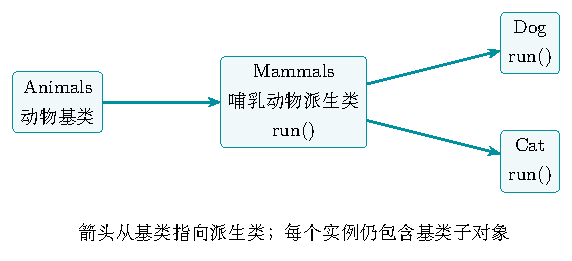
\includegraphics[width=0.7\textwidth]{inheritance_revised.pdf}
    \caption{类的继承} % 图片标题
    \label{fig:A111} % 图片标签，用于引用
\end{figure}

如图\ref{fig:A111}所示，派生类从基类中继承了数据成员和成员函数，并可以添加新的成员。
派生类可以重写基类中的成员虚函数，从而实现新的功能。
派生类可以重载基类中的运算符，从而实现新的运算。

下面按 public 继承、普通成员访问来比较（友元按授权另行处理）。protected 的派生类访问还受对象类型等规则约束，不能理解成对任意基类对象都随意访问。
这张表和"类的基本概念"中的是同一张，这里从继承的视角再看一次——重点关注"派生类"这一行：

\begin{center}
    \begin{tabular}{cccc}
        \toprule[1.5pt]
        访问位置 & public 成员 & private 成员 & protected 成员 \\
        \midrule[1pt]
        同一个类 & yes & yes & yes \\
        派生类 & yes & no & yes \\
        类外部 & yes & no & no \\
        \bottomrule[1.5pt]
    \end{tabular}
\end{center}

继承可以用下面的写法实现：

\Needspace{9\baselineskip}
\begin{example}
抽象基类与两个派生类：
\lstinputlisting[language=C++,numbers=left,numberstyle={\color{gray}\tiny}]{examples/class-basics-demo/inheritance.cpp}


从本卷目录进入 \path{examples/class-basics-demo}，保存的源码就是 \texttt{inheritance.cpp}。
\begin{tbash}
g++ -std=c++17 -Wall -Wextra -pthread inheritance.cpp -o /tmp/cpp-demo
/tmp/cpp-demo
\end{tbash}
先看到基类、再看到派生类的构造提示；下一道练习会通过基类指针调用面积函数。
\end{example}

\begin{note}
继承方式有三种：\texttt{public}、\texttt{protected}、\texttt{private}（\texttt{class} 默认 private，\texttt{struct} 默认 public），
它决定了基类成员在派生类中的访问权限上限。工程中绝大多数情况都用 \texttt{public} 继承，
另外两种仅作了解。含纯虚函数的抽象类不能直接实例化，只能作为基类使用。

另外注意初始化列表的写法：\textbf{基类构造函数写在成员之前}，成员之间按\textbf{声明顺序}初始化，
与列表里的书写顺序无关。写错顺序编译器会发出 \texttt{-Wreorder} 警告，如果成员之间存在初始化依赖，还会得到未定义的值。
\end{note}

\begin{conclusion}
重载（overload）与重写（override）仅一字之差，但完全是两回事：

\begin{itemize}
\item 重载 overload：同一作用域内的同名函数，参数列表不同，编译期由编译器选择版本，与继承无关；
\item 重写 override：派生类重新实现基类的 \texttt{virtual} 函数，函数签名必须相同，通过基类指针或引用调用时，根据对象实际类型决定调用哪个版本（多态），建议显式标注 \texttt{override} 让编译器帮忙检查；
\item 纯虚函数 \texttt{= 0}：基类只给接口不给实现，仍有纯虚函数没有最终实现的类是抽象类，不能实例化。纯虚函数也能在类外提供定义，这里先只把它作为接口使用。
\end{itemize}
\end{conclusion}

\begin{exercise}\label{ex:v1-cpp-inheritance}

在上例基础上，于 \texttt{main} 中创建 \texttt{Shape*} 数组分别指向 \texttt{Circle} 和 \texttt{Rectangle} 对象，
循环调用 \texttt{calArea()}，观察多态的调用结果。
\end{exercise}

 \subsubsection{模板}
在开发过程中，我们可能会遇到这样的场景：我们有一个函数或者类，但是它只适用于特定的数据类型，
比如\texttt{int}或者\texttt{double}。为了让这两种类型都可以调用函数，
就得把代码复制一遍，但这样做就造成了代码冗余，不利于维护。这时候就需要用到模板（\texttt{template}）。

模板是C++中一个重要的特性，它允许我们定义一个类或函数，使其可以接受不同的数据类型或者不同的参数。
模板的定义和使用都比较复杂，这里只介绍最基本的用法。
\textbf{函数模板}用 \texttt{template} 加尖括号声明一个类型参数（习惯命名为 \texttt{T}），之后 \texttt{T} 就可以像普通类型一样使用。语法如下：
\begin{tcode}
template<class T>
T function(T a){
    return a;
}
\end{tcode}

这里的\texttt{class T}表示一种数据类型，可以是任意类型。
在函数的定义中，\texttt{T}可以作为函数的参数，也可以作为函数的局部变量。在使用函数模板时，需要首先进行函数的实例化。

\Needspace{9\baselineskip}
\begin{example}
函数模板的实例化与调用：
\lstinputlisting[language=C++,numbers=left,numberstyle={\color{gray}\tiny}]{examples/class-basics-demo/function-template.cpp}


从本卷目录进入 \path{examples/class-basics-demo}，保存的源码就是 \texttt{function-template.cpp}。
\begin{tbash}
g++ -std=c++17 -Wall -Wextra -pthread function-template.cpp -o /tmp/cpp-demo
/tmp/cpp-demo
\end{tbash}
这里输出 1 和 10。实例化把模板参数换成具体类型，调用才执行函数体。
\end{example}

模板的优点：
\begin{enumerate}
    \item 代码重用性高：可以定义一个通用的函数，然后根据需要实例化不同的类型，实现代码的重用。
    \item 类型安全：不符合类型要求的用法通常能在编译时发现，而不是等运行时猜数据是什么。
    \item 效率高：编译器可以针对具体类型优化；实际速度仍要看算法与使用方式。
\end{enumerate}

\textbf{类模板}：
类模板的语法和函数模板类似，只不过在类名而不是函数名前面加上关键字\texttt{template}。
在普通类中也可以添加成员函数模板，只需要在函数名前面加上关键字\texttt{template}即可。

\Needspace{9\baselineskip}
\begin{example}
类模板的基本写法：
\lstinputlisting[language=C++,numbers=left,numberstyle={\color{gray}\tiny}]{examples/class-basics-demo/class-template.cpp}


从本卷目录进入 \path{examples/class-basics-demo}，保存的源码就是 \texttt{class-template.cpp}。
\begin{tbash}
g++ -std=c++17 -Wall -Wextra -pthread class-template.cpp -o /tmp/cpp-demo
/tmp/cpp-demo
\end{tbash}
这里输出 1 2.5，同一个类模板按两个类型参数组成了这个对象。
\end{example}

模板参数除了类型，还可以是\textbf{编译期常量}（非类型模板参数），常用于指定数组长度这类编译期就要确定的值：

\Needspace{9\baselineskip}
\begin{example}
非类型模板参数：
\lstinputlisting[language=C++,numbers=left,numberstyle={\color{gray}\tiny}]{examples/class-basics-demo/constant-template.cpp}


从本卷目录进入 \path{examples/class-basics-demo}，保存的源码就是 \texttt{constant-template.cpp}。
\begin{tbash}
g++ -std=c++17 -Wall -Wextra -pthread constant-template.cpp -o /tmp/cpp-demo
/tmp/cpp-demo
\end{tbash}
这里输出 42，N 在编译时已经确定。
\end{example}

在\texttt{template}后面，可以定义多个类型参数，用逗号分隔。需要注意的是，类中的函数模板需要在头文件中实现，
这使编译器在需要实例化时看得到定义。也可以显式实例化后分离编译，但初学阶段先把定义放进头文件，省去链接时找不到实现的麻烦。
对于类模板也可以实现继承和多态，与普通类相同，这里不再展开，感兴趣的同学可以自行探索。

\textbf{模板的实例化}：
模板的实例化指的是将模板定义和具体的模板参数绑定在一起，生成一个具体的类或函数。
写 \texttt{A<int, double>} 时，编译器会根据尖括号里的参数生成对应的版本。模板参数可以填两类东西：

\begin{enumerate}
    \item 具体类型：如\texttt{int}、\texttt{double}等基本类型，\texttt{struct}、\texttt{class}、\texttt{union}等复合类型，以及指针和引用类型；
    \item 编译期可以确定的常量：字面常量、宏、\texttt{constexpr}，对应上面的非类型模板参数。
\end{enumerate}

平时我们写的 \texttt{function<int>(10)} 其实叫\textbf{隐式实例化}——用到时才生成；
也可以在代码里写 \texttt{template class A<int, double>;} 主动要求编译器立刻生成，这叫\textbf{显式实例化}，
常用于模板分离编译的场景，初学阶段了解即可。

除此之外，还有一种变参模板，它可以接受任意数量的类型参数，但是在实例化时，必须指定具体的类型。
这种情况比较复杂，这里不再展开。

\begin{note}
对变参模板感兴趣的同学可以自行探讨：

\url{https://blog.csdn.net/fl2011sx/article/details/128077440}
\end{note}

\begin{exercise}\label{ex:v1-cpp-template}

编写函数模板 \texttt{myMax}，返回两个同类型参数中较大的一个，分别用 \texttt{int}、\texttt{double} 测试，
并尝试用 \texttt{myMax(1, 2.5)} 调用，观察编译器的报错信息，思考为什么。再运行 class-template.cpp 与 constant-template.cpp，分别指出类型参数与非类型参数；不能把运行时读入的整数直接当成编译期 N。
\end{exercise}


\section{Lambda 表达式、引用与移动}
随着时代的发展和项目变得越来越复杂，人们创造了一系列新的代码特性，其中一些特性在C++11和C++17中被引入，
在不熟悉这些特性的人看来，这些代码看上去显得十分无厘头，甚至有些难以理解。本节将介绍C++11和C++17中引入的一些新的代码特性，
并通过实例来说明它们的用法。

\subsubsection{lambda表达式}

\textbf{匿名函数（anonymous function）}是一种在程序中定义的函数，它没有普通函数那样的名字。C++11引入了lambda表达式，
它是一种更简洁的语法，可以用来创建匿名函数。lambda表达式的语法如下：

\begin{tcode}
常见形式：[捕获列表](参数列表) mutable noexcept -> 返回类型 {函数体}
简化版：[捕获列表](参数列表) {函数体}
\end{tcode}

\begin{enumerate}
    \item 捕获列表：捕获列表可以用来捕获外部作用域中的变量，使得lambda表达式可以访问这些变量。
    \item 参数列表：参数列表定义了lambda表达式的参数，可以有0到多个参数。
    \item mutable[可选]：mutable 允许修改值捕获的副本，不会自动修改原变量。
    \item noexcept[可选]：声明调用不会抛出异常；违反承诺会终止程序。旧的 throw(类型列表) 已在 C++17 中移除，这里不用它。
    \item 返回值：返回值定义了lambda表达式的返回类型，编译器一般可以自动推导，可以省略。
    \item 函数体：函数体定义了lambda表达式的主体，可以是一条表达式或多条语句。
\end{enumerate}

刚才的函数都起了名字，接下来会遇到“把一段行为交给另一个函数”的写法。我们把排序、捕获与移动分成独立程序，一次只看一个区别。项目放在 \path{examples/lambda-move-demo}，文件组成如下。每个 cpp 都有自己的 main，分别编译；不要把它们拼成一个文件。
\begin{lstlisting}[language={}]
lambda-move-demo/
  README.md
  capture.cpp
  forward.cpp
  function.cpp
  move-construction.cpp
  move-overloads.cpp
  mutable.cpp
  reference.cpp
  rvalue-reference.cpp
  sort.cpp
\end{lstlisting}
编译命令里，-std 指定 C++ 标准，-Wall/-Wextra 打开常用警告，-pthread 配置线程编译与链接；-o 指定临时输出文件。先进入项目目录，后面的源码名按当前示例替换。

\Needspace{9\baselineskip}
\begin{example}
用 lambda 作为比较器，对自定义结构体数组排序：
\lstinputlisting[language=C++,numbers=left,numberstyle={\color{gray}\tiny}]{examples/lambda-move-demo/sort.cpp}


从本卷目录进入 \path{examples/lambda-move-demo}，保存的源码就是 \texttt{sort.cpp}。
\begin{tbash}
g++ -std=c++17 -Wall -Wextra -pthread sort.cpp -o /tmp/cpp-demo
/tmp/cpp-demo
\end{tbash}
先输出和 3，再看到 id 依次为 7、4、2、1、-1；比较器决定了降序规则。
\end{example}

\textbf{捕获列表：}可以捕获外部作用域中的变量，包括this指针。捕获的方式包括两种，即值捕获和引用捕获。

\begin{center}
    \begin{tabular}{cccc}
        \toprule[1.5pt]
        捕获方式 & 拷贝方式 & 是否可以修改值 & 语法示例 \\
        \midrule[1pt]
        值捕获 & 保存副本 & 默认不能改副本 & [a,b]，全捕获 [=] \\
        引用捕获 & 引用原对象 & 原对象可修改时可以 & [\&a,\&b]，全捕获 [\&] \\
        \bottomrule[1.5pt]
    \end{tabular}
\end{center}

值捕获保存的是变量的副本，具体复制什么取决于类型。例如捕获一个指针，只复制地址，不会顺便复制它指向的对象。
默认的调用运算符是 const，所以不能修改捕获的普通整数副本；加上 mutable 后可以改副本，原整数仍不受影响。
引用捕获则直接使用原对象，不过你要保证调用时它还活着，不能把引用局部变量的 lambda 留到函数返回后再调用。

\Needspace{9\baselineskip}
\begin{example}
mutable 与值捕获：
\lstinputlisting[language=C++,numbers=left,numberstyle={\color{gray}\tiny}]{examples/lambda-move-demo/mutable.cpp}


从本卷目录进入 \path{examples/lambda-move-demo}，保存的源码就是 \texttt{mutable.cpp}。
\begin{tbash}
g++ -std=c++17 -Wall -Wextra -pthread mutable.cpp -o /tmp/cpp-demo
/tmp/cpp-demo
\end{tbash}
输出 1 0：被加一的是副本，外面的 a 仍是 0。
\end{example}

使用lambda表达式可以简化代码，提高可读性。由于捕获列表的存在，使得lambda表达式可以访问外部作用域的变量，
相比于普通函数，lambda表达式更加灵活。
lambda表达式的本质是一个\textbf{匿名的函数对象}（闭包），可以用 \texttt{auto} 或 \texttt{std::function} 承接；
没有任何捕获的 lambda 还可以隐式转换为函数指针，作为函数参数进行传递。

\Needspace{9\baselineskip}
\begin{example}
用 \texttt{std::function} 和 \texttt{auto} 承接 lambda：
\lstinputlisting[language=C++,numbers=left,numberstyle={\color{gray}\tiny}]{examples/lambda-move-demo/function.cpp}


从本卷目录进入 \path{examples/lambda-move-demo}，保存的源码就是 \texttt{function.cpp}。
\begin{tbash}
g++ -std=c++17 -Wall -Wextra -pthread function.cpp -o /tmp/cpp-demo
/tmp/cpp-demo
\end{tbash}
输出 3 1；两种变量都能保存可调用对象，auto 并不是“自动推导函数的返回值”。
\end{example}

在C++14和C++17中，lambda表达式增加了一些新的用法，使用这些新的特性可以简化代码，更加灵活地解决实际问题。

\textbf{泛型Lambda表达式：}
可以使用auto关键字指定形参的类型，从而快速地实现函数\textbf{泛用}。这也是\textbf{泛化编程}的一种方式，感兴趣的同学可以自行了解。
\begin{tcode}
auto f=[](auto a,auto b){return a+b;};
std::cout << f(1,2) << " " << f('a',2.0) << std::endl;
\end{tcode}

\textbf{this指针捕获：}
可以用 [this] 保存当前对象的指针，也可以从 C++17 起用 [*this] 保存当前对象的副本。两者不一样：对象后来变了，前者会看到新值，后者仍使用捕获时的副本。先看指针捕获的片段，完整对照见后面的捕获项目：
\begin{tcode}
class A{
private:
    int a = 1;
public:
    A(){
        auto function = [this](){//保存this指针，调用时对象须仍存活
            return a+1;
        };
    }
};
\end{tcode}

\textbf{初始化捕获：}在C++14中，可以使用初始化捕获来简化代码。
可以初始化一个变量，并将其绑定到lambda表达式中，这样就不需要再声明这个变量了。

\begin{tcode}
auto f = [a=1]() mutable {
    return a;
};
\end{tcode}


\Needspace{10\baselineskip}
\begin{example}
项目的 \texttt{capture.cpp} 把捕获的区别放在一起。先保存两个 lambda，再修改对象，这时候看看它们分别读到了谁：
\lstinputlisting[language=C++,numbers=left,numberstyle={\color{gray}\tiny}]{examples/lambda-move-demo/capture.cpp}
\begin{tbash}
g++ -std=c++17 -Wall -Wextra capture.cpp -o /tmp/capture-demo
/tmp/capture-demo
\end{tbash}
前两行是 2 1、2：mutable 改副本，引用捕获改原整数。最后是 5 1：保存 this 指针的 lambda 看到修改后的对象，保存 *this 副本的 lambda 看到旧值。本例对象一直活到调用结束；指针捕获不会替它延长寿命。
\end{example}
\begin{exercise}
\label{ex:v1-cpp-capture}
在 capture.cpp 中把对象的新值改为 9，先预测两种对象捕获的输出，再运行核验；解释为什么不能把保存 this 指针的 lambda 留到对象析构后使用。
\end{exercise}
\begin{exercise}\label{ex:v1-cpp-sort}

使用 \texttt{std::sort}（头文件 \texttt{<algorithm>}）配合 lambda 比较器，把一个 \texttt{std::vector<int>}
先按升序排序、再按降序排序，分别打印结果。
\end{exercise}

\subsubsection{引用和移动}
\textbf{左值与右值：}
先别急着按“等号左边、等号右边”来记，值类别描述的是\textbf{表达式}。普通变量名、解引用表达式通常是左值（lvalue），它们能指明已有对象；整数字面量和普通计算结果通常是纯右值（prvalue），例如 10 和 a+1。还有一种将亡值（xvalue），例如 \texttt{std::move(a)}：它仍指明已有对象，但允许后续操作复用其资源。纯右值与将亡值统称右值（rvalue）。

对普通整数，能否取地址可以帮助判断，但不是定义：位域是左值却不能取地址，字符串字面量也是左值；右值也不一定不可修改，例如临时类对象可以调用修改自身的成员函数。别把“临时”与“常量”混在一起。临时对象通常在完整表达式结束时销毁，满足条件的引用绑定可以延长其寿命，下面就来看这个区别。
\begin{tcode}
int a;
a = 10;//这个赋值过程中，a是左值，10是右值（字面常量）
int b;
b = a;//这个赋值过程中，b是左值，a是左值（左值可以作为右值使用）
//10 = a;//这样的语句显然是错误的，即右值不能被修改
\end{tcode}
把 a 放在赋值右边，只是在这里读取它的值，a 这个表达式本身仍是左值；值类别不由它在等号哪边决定。

\textbf{引用：}
C++的引用是一种别名，用于引用已存在的变量。引用一旦初始化，就不能再引用其他变量。引用不会为被引用对象再复制一份数据，底层是否需要保存地址由实现决定。
引用的主要用途包括函数参数传递和返回值优化。使用引用可以避免复制，提高效率，特别是在处理大型对象时。
引用通过 \& 符号来声明。例如:
\begin{tcode}
int& ref = var;
\end{tcode}
这段代码创建了一个名为 \texttt{ref} 的引用，它引用了变量 \texttt{var}。引用分为两种，左值引用（\&）和右值引用（\&\&）。
普通 \texttt{T\&} 绑定左值，\texttt{const T\&} 还可以绑定临时对象。普通 \texttt{T\&\&} 绑定右值；模板参数推导中的转发引用另有规则，稍后单独讲。

首先说左值引用，这个十分简单，可以认为是取别名，操作左值引用就相当于操作被绑定的那个左值本身，这一点就算在函数传参过程中也是如此。
\Needspace{9\baselineskip}
\begin{example}
左值引用传参：
\lstinputlisting[language=C++,numbers=left,numberstyle={\color{gray}\tiny}]{examples/lambda-move-demo/reference.cpp}


从本卷目录进入 \path{examples/lambda-move-demo}，保存的源码就是 \texttt{reference.cpp}。
\begin{tbash}
g++ -std=c++17 -Wall -Wextra -pthread reference.cpp -o /tmp/cpp-demo
/tmp/cpp-demo
\end{tbash}
输出 20，引用参数修改了 main 中的整数。
\end{example}
在这里a的值被修改为20，因为传入\texttt{func()}的a是引用，所以操作的是a本身，而不是a的拷贝。
这就是引用在传参和提高函数效率上的用处。

再说右值引用，这个就有点复杂了，右值引用是为了解决左值引用不能绑定右值的限制。
\Needspace{9\baselineskip}
\begin{example}
右值引用绑定右值：
\lstinputlisting[language=C++,numbers=left,numberstyle={\color{gray}\tiny}]{examples/lambda-move-demo/rvalue-reference.cpp}


从本卷目录进入 \path{examples/lambda-move-demo}，保存的源码就是 \texttt{rvalue-reference.cpp}。
\begin{tbash}
g++ -std=c++17 -Wall -Wextra -pthread rvalue-reference.cpp -o /tmp/cpp-demo
/tmp/cpp-demo
\end{tbash}
c 从 10 变为 20，地址由本次运行决定；这个修改本身没有发生资源移动。
\end{example}

咦？c 明明绑定了一个右值，为什么能取到地址、还能被修改？

原因在于两点：一是这里直接用临时值初始化局部右值引用，临时对象的寿命被延长到了这个引用的作用域结束；
二是\textbf{有名字的右值引用本身会被当作左值来使用}——既然有名字，就能取地址、能修改，用起来和普通左值引用没有区别。

那右值引用存在的意义是什么？设想一个超级大的对象：传出函数时，我们希望把它的资源交给新对象，避免不必要的复制。实际返回还可能经过返回值优化，不能把所有返回都算成复制。
右值引用让我们可以直接"接管"临时对象的内存，避免这次拷贝——具体能否转移、怎样转移，由类型的移动构造或移动赋值实现决定。仅仅绑定右值引用，并不会替你搬数据。
这就是移动构造函数存在的理由，马上就能在下面的例子里看到。

\Needspace{9\baselineskip}
\begin{example}
一个演示默认、含参、拷贝、移动构造与拷贝赋值的类（不代表写全了所有特殊成员函数），请仔细体会每一行的输出：
\lstinputlisting[language=C++,numbers=left,numberstyle={\color{gray}\tiny}]{examples/lambda-move-demo/move-construction.cpp}


从本卷目录进入 \path{examples/lambda-move-demo}，保存的源码就是 \texttt{move-construction.cpp}。
\begin{tbash}
g++ -std=c++17 -Wall -Wextra -pthread move-construction.cpp -o /tmp/cpp-demo
/tmp/cpp-demo
\end{tbash}
对照上面的执行顺序检查构造、赋值和析构记录。
\end{example}
这时候回头看 a5 和 a6：a5 只是给 a1 多取了一个别名，没有调用移动构造；a6 才创建新对象并调用移动构造。移动后的字符串仍有效，但内容不保证一定为空，不要把某次输出当成固定规则。

\textbf{移动语义：}
首先了解一个std中的函数move，它的作用是将参数类型强制转换为右值，不管参数原来是左值还是右值。
\Needspace{9\baselineskip}
\begin{example}
\texttt{std::move} 的效果：
\lstinputlisting[language=C++,numbers=left,numberstyle={\color{gray}\tiny}]{examples/lambda-move-demo/move-overloads.cpp}


从本卷目录进入 \path{examples/lambda-move-demo}，保存的源码就是 \texttt{move-overloads.cpp}。
\begin{tbash}
g++ -std=c++17 -Wall -Wextra -pthread move-overloads.cpp -o /tmp/cpp-demo
/tmp/cpp-demo
\end{tbash}
调用类别依次是右值、左值、右值、const 左值、const 右值。
\end{example}
如代码所见，当我们使用std::move()时，编译器将左值转换为右值。

再介绍一种利用模板实现完美转发的方式。在模板中，T\&\&可以接收左值和右值，要利用到forward<>()函数，它会保留引用的类型，并将其转发给另一个函数，
因为有名字的参数 t 在函数体中是左值表达式，直接传 t 会选择左值重载。这里的 T 必须是被推导的模板参数；并非所有 T\&\& 都是转发引用。

\Needspace{9\baselineskip}
\begin{example}
完美转发：
\lstinputlisting[language=C++,numbers=left,numberstyle={\color{gray}\tiny}]{examples/lambda-move-demo/forward.cpp}


从本卷目录进入 \path{examples/lambda-move-demo}，保存的源码就是 \texttt{forward.cpp}。
\begin{tbash}
g++ -std=c++17 -Wall -Wextra -pthread forward.cpp -o /tmp/cpp-demo
/tmp/cpp-demo
\end{tbash}
先运行原版，再按紧邻的提示替换 Fun(t)，比较两次记录。只有后者会保留右值调用类别。
\end{example}

\begin{note}
先运行 \texttt{Fun(t)}，再把这一行换成 \texttt{Fun(std::forward<T>(t))}，不要两行同时保留。对比调用记录：前者把有名字的参数作为左值传入，后者保留传入时的值类别。引用折叠是类型规则，与表达式有名字后成为左值要分开看。
\end{note}

\begin{conclusion}
左值、右值与两种引用的对照：

\begin{itemize}
\item 值类别属于表达式：变量名通常是左值，10 是纯右值，std::move(x) 是将亡值；不要只按取地址或等号位置判断；
\item 普通 T\& 绑定左值，const T\& 还能绑定临时对象；引用必须在对象有效期内使用；
\item 普通 T\&\& 绑定右值，有名字的右值引用作为表达式仍是左值；绑定本身不转移资源；
\item \texttt{std::move}：把左值强制转成右值（本身不移动任何数据），\texttt{std::forward}：在模板中保留参数的左右值属性。
\end{itemize}
\end{conclusion}

左值引用和右值引用的概念比较容易混淆，要在实践中不断运用，才能熟练掌握。

\begin{exercise}\label{ex:v1-cpp-reference}

编写一个函数 \texttt{void swapVal(int\& a, int\& b)} 交换两个整数的值，在 \texttt{main} 中调用并验证；
再把参数类型改为按值传递（去掉 \texttt{\&}），观察交换是否仍然生效，解释原因。再对照 move-construction.cpp 的 a5、a6，说明哪一处真正调用了移动构造；按提示切换 forward.cpp 的调用语句，预测并核验五次重载选择。
\end{exercise}


\section{智能指针}
动态内存若使用 $new$/$delete$ 手动管理，易因遗漏释放导致内存泄漏；在对象生命周期复杂、函数嵌套较深时尤甚。C++11 引入智能指针，在对象析构时自动释放所管理的堆内存。常用类型包括 $unique\_ptr$、$shared\_ptr$ 与 $weak\_ptr$。

下文示例中的类型 $A$、$B$ 定义如下。

\begin{tcode}
class A;
class B;
class A{
public:
    A(){std::cout << "你调用了A的默认构造函数" << std::endl;}
    ~A(){std::cout << "A对象已被析构，val值为：" << val << std::endl;}
    int getVal(){return val;};
    void setVal(int val){this->val = val;}
    std::shared_ptr<B> B_ptr;
private:
    int val;
};

class B{
public:
    B(){std::cout << "你调用了B的默认构造函数" << std::endl;}
    ~B(){std::cout << "B对象已被析构，val值为：" << val << std::endl;}
    int getVal(){return val;};
    void setVal(int val){this->val = val;}
    std::weak_ptr<A> A_ptr; //注意：这里是weak_ptr，不是shared_ptr
private:
    int val;
};
\end{tcode}

\subsubsection{unique\_ptr}
$unique\_ptr$ 为独占式智能指针：同一时刻仅允许一个指针拥有资源。离开作用域时自动释放资源。拷贝构造与拷贝赋值被禁用，所有权只能通过移动转移。

\begin{example}
\texttt{unique\_ptr} 的所有权转移：
\begin{tcode}
#include <iostream>
#include <memory>

int main() {
    {
        std::unique_ptr<A> ptr1 = std::make_unique<A>();
        ptr1->setVal(1);
        //std::unique_ptr<A> ptr2 = ptr1;会报错，独占指针不允许拷贝
        std::unique_ptr<A> ptr2 = std::move(ptr1);
        if(ptr1 == nullptr){
            std::cout << "ptr1是一个空指针" << std::endl;
        }
        std::cout << "ptr2的val值为：" << ptr2->getVal() << std::endl;
        ptr1 = std::make_unique<A>();
        ptr1->setVal(2);
    }//离开作用域，ptr1和ptr2管理的对象被自动析构
    return 0;
}
\end{tcode}
\end{example}

\begin{note}
创建智能指针优先使用 \texttt{std::make\_unique} / \texttt{std::make\_shared}，而不是先 \texttt{new} 再交给智能指针接管。
前者一步完成，更安全也更高效；手动 \texttt{new} 出来的原始指针一旦被两个智能指针同时接管，会被析构两次，直接崩溃。
\end{note}

\begin{exercise}
编写函数 \texttt{std::unique\_ptr<A> create(int v)}，在堆上创建一个 \texttt{A} 对象、设置 \texttt{val} 为 \texttt{v} 并返回；
在 \texttt{main} 中接收返回值并打印 \texttt{val}。思考：为什么这里返回 \texttt{unique\_ptr} 不需要担心拷贝被禁用？
\end{exercise}

\subsubsection{shared\_ptr}
当需要多个指针共同管理同一资源时，应使用 $shared\_ptr$。其内部维护引用计数：拷贝使计数加一，析构使计数减一；计数归零时释放资源。移动操作转移所有权，不增加引用计数。

\begin{example}
观察引用计数的变化：
\begin{tcode}
#include <iostream>
#include <memory>

int main() {
    {
        std::shared_ptr<A> ptr1 = nullptr;
        {
            auto ptr2 = std::make_shared<A>();
            ptr2->setVal(1);
            ptr1 = ptr2;
            //ptr1 = std::move(ptr2);//看一下这两种写法有什么区别？
            std::cout << "ptr1对象的引用次数为：" << ptr1.use_count() << std::endl;
            std::cout << "ptr2对象的引用次数为：" << ptr2.use_count() << std::endl;
        }
        std::cout << "ptr2已经被析构了" << std::endl;
        std::cout << "但A对象还活着，引用次数为：" << ptr1.use_count() << std::endl;
    }//到这里A对象才被析构
    return 0;
}
\end{tcode}
\end{example}

\subsubsection{循环引用与 weak\_ptr}
若两个 $shared\_ptr$ 互相持有对方，将形成循环引用，引用计数无法归零，对象无法析构，从而造成泄漏。

\begin{example}
循环引用演示（先把 B 类中的 \texttt{A\_ptr} 临时改回 \texttt{shared\_ptr<A>} 再运行）：
\begin{tcode}
int main(int argc, char *argv[]) {
    {
        std::shared_ptr<A> pA(new A);
        std::shared_ptr<B> pB(new B);

        std::cout << pA.use_count() << std::endl;
        std::cout << pB.use_count() << std::endl;
    }
    std::cout << "上面是符合我们预期的" << std::endl << std::endl;
    {
        std::shared_ptr<A> pA(new A);
        std::shared_ptr<B> pB(new B);

        pA->B_ptr = pB;
        pB->A_ptr = pA;

        std::cout << pA.use_count() << std::endl;
        std::cout << pB.use_count() << std::endl;
    }
    std::cout << "咦？这是什么情况呢？为什么没有被析构呢？" << std::endl;
    return 0;
}
\end{tcode}
\end{example}

此时应将一侧改为 $weak\_ptr$（正如本节开头 B 类中的写法）。$weak\_ptr$ 不增加引用计数，也不直接解引用资源；需要访问时通过 $lock()$ 升级为 $shared\_ptr$，并检查返回值是否为空。

\begin{example}
用 \texttt{weak\_ptr} 打破循环引用：
\begin{tcode}
int main() {
    {
        std::shared_ptr<A> pA(new A);
        std::shared_ptr<B> pB(new B);

        pA->B_ptr = pB;
        pB->A_ptr = pA; //weak_ptr不增加引用计数

        std::cout << pA.use_count() << std::endl;
        std::cout << pB.use_count() << std::endl;

        std::shared_ptr<A> PtrA = pB->A_ptr.lock(); //升级为shared_ptr再使用
        if(PtrA != nullptr)
            PtrA->setVal(1234);
        PtrA.reset();
    }//这次两个对象都能正常析构了
    return 0;
}
\end{tcode}
\end{example}

在多线程环境下，$lock()$ 可用于在访问前确认共享对象仍存活。相关同步问题见多线程章节。

\begin{exercise}
运行"循环引用演示"示例，观察两段的析构输出差异；然后保持 \texttt{weak\_ptr} 写法再运行一遍，
确认两个对象都能正常析构，并用自己的话解释原因。
\end{exercise}

\subsubsection{三种智能指针对照}
\begin{conclusion}
\begin{center}
    \begin{tabular}{cccc}
        \toprule[1.5pt]
        智能指针 & 指向数量 & 析构条件 & 是否可操作资源\\
        \midrule[1pt]
        unique\_ptr & 只能一个 & 离开作用域 & 是\\
        shared\_ptr & 可多个指向同一对象 & 引用计数为 0 & 是\\
        weak\_ptr & 可观察 shared\_ptr 管理的对象 & 不单独决定析构 & 否，需 lock 升级\\
        \bottomrule[1.5pt]
    \end{tabular}
\end{center}

选择原则：默认用 \texttt{unique\_ptr}；确实需要共享所有权时才用 \texttt{shared\_ptr}；
只想"看一眼"而不想延长对象寿命时用 \texttt{weak\_ptr}。这就好比宿舍钥匙：独居一把钥匙（unique），
合租人手一把、最后走的人锁门（shared），访客只登记不配钥匙（weak）。
\end{conclusion}

最后补充说明循环引用的两种形态，它们的处理难度完全不同：

\begin{itemize}
\item \textbf{静态环}：像本节 A、B 两个类这样，互相持有的关系在代码里写得明明白白。
这种环一眼就能看出来，设计时把一侧改成 \texttt{weak\_ptr} 即可解决；
\item \textbf{动态环}：环是在运行过程中"长"出来的——比如用 \texttt{shared\_ptr} 组织的链表、图结构，
随着数据不断增加，节点之间可能意外连成一个环。这种环在代码里看不到，等到内存泄漏时往往已经很难排查。
\end{itemize}

\begin{note}
对于动态环，标准库\textbf{没有}通用的解决方案：\texttt{weak\_ptr} 只能破解你预先知道存在的那条边，
而运行时才形成的环你根本不知道该在哪一侧用 \texttt{weak\_ptr}。
工程上的应对办法是在设计阶段就规定好所有权方向（比如父子结构中父持有子、子用 \texttt{weak\_ptr} 回指父），
并通过代码评审和内存检测工具（如 AddressSanitizer 的泄漏检查）来兜底。
\end{note}


\section{标准模版库（STL）}
本节介绍常用数据结构对应的 STL 容器，以及迭代器的基本用法与失效问题。
\subsubsection{数据结构概览}

所谓数据结构，就是指数据的组织、存储、操作和处理方式。数据结构是计算机科学中最基本的概念之一，
是计算机程序设计的基础。基本的操作有四：\textbf{插入、删除、改动、查找}（增删改查）。

下面我们将简单介绍几种常见的数据结构，以及它们的STL容器：

\begin{enumerate}
    \item \textbf{数组（Array）}：相同类型的元素按顺序存储在一块连续内存中的线性结构，
    可以通过下标在 $O(1)$ 时间内直接访问任意元素。
    \item \textbf{链表（Linked List）}：由一系列在内存中不连续的节点串成的线性结构，
    每个节点存储数据和指向下一个节点的指针；已知位置时插入、删除只需改变指针，
    但查找必须从头节点开始逐个遍历。
    \item \textbf{队列（Queue）}：先进先出（FIFO，First In First Out）的线性结构，
    只允许在队尾插入元素、在队头删除元素，先进入的元素先被取出。
    \item \textbf{优先队列（Priority Queue）}：每个元素都带有一个优先级的队列，
    每次出队的不是最早进入的元素，而是当前优先级最高的元素。
    \item \textbf{堆栈（Stack）}：后进先出（LIFO，Last In First Out）的线性结构，
    插入（压栈）和删除（弹栈）都只能在栈顶一端进行。
    \item \textbf{树（Tree）}：一种非线性结构，其中有且仅有一个根节点，
    其余每个节点都恰好有一个父节点；任意两个节点之间有且仅有一条路径相连，即树中不存在环路。
    \item \textbf{二叉树（Binary Tree）}：每个节点至多有两个子节点的树，
    两个子节点区分左右，分别称为左子节点和右子节点。
    \item \textbf{堆（Heap）}：满足"堆性质"的完全二叉树——最大堆中每个节点的值都大于或等于其子节点，
    最小堆则相反；因此堆顶永远是最大值（或最小值）。
\end{enumerate}

它们的头文件如下：

\begin{tcode}
#include <array>    //静态数组array
#include <vector>   //动态数组vector
#include <list>     //链表list
#include <queue>    //队列queue 优先队列priority_queue
#include <stack>    //堆栈stack
#include <map>      //映射map 是一种快速查找关联容器
\end{tcode}

需要注意的是，上面所列举的数据结构类型并不是并列的，三大数据结构分别是：线性表（包括1、2、3、4、5）
，树（包括6、7、8），图（太复杂，暂时不介绍）。

\subsubsection{顺序容器}
\textbf{数组与 vector。}

数组是最基本的数据结构，它是一组相同类型的数据，按照顺序存储在一块连续的内存中，如图\ref{fig:数组}。

\begin{figure}[H]
    \centering
    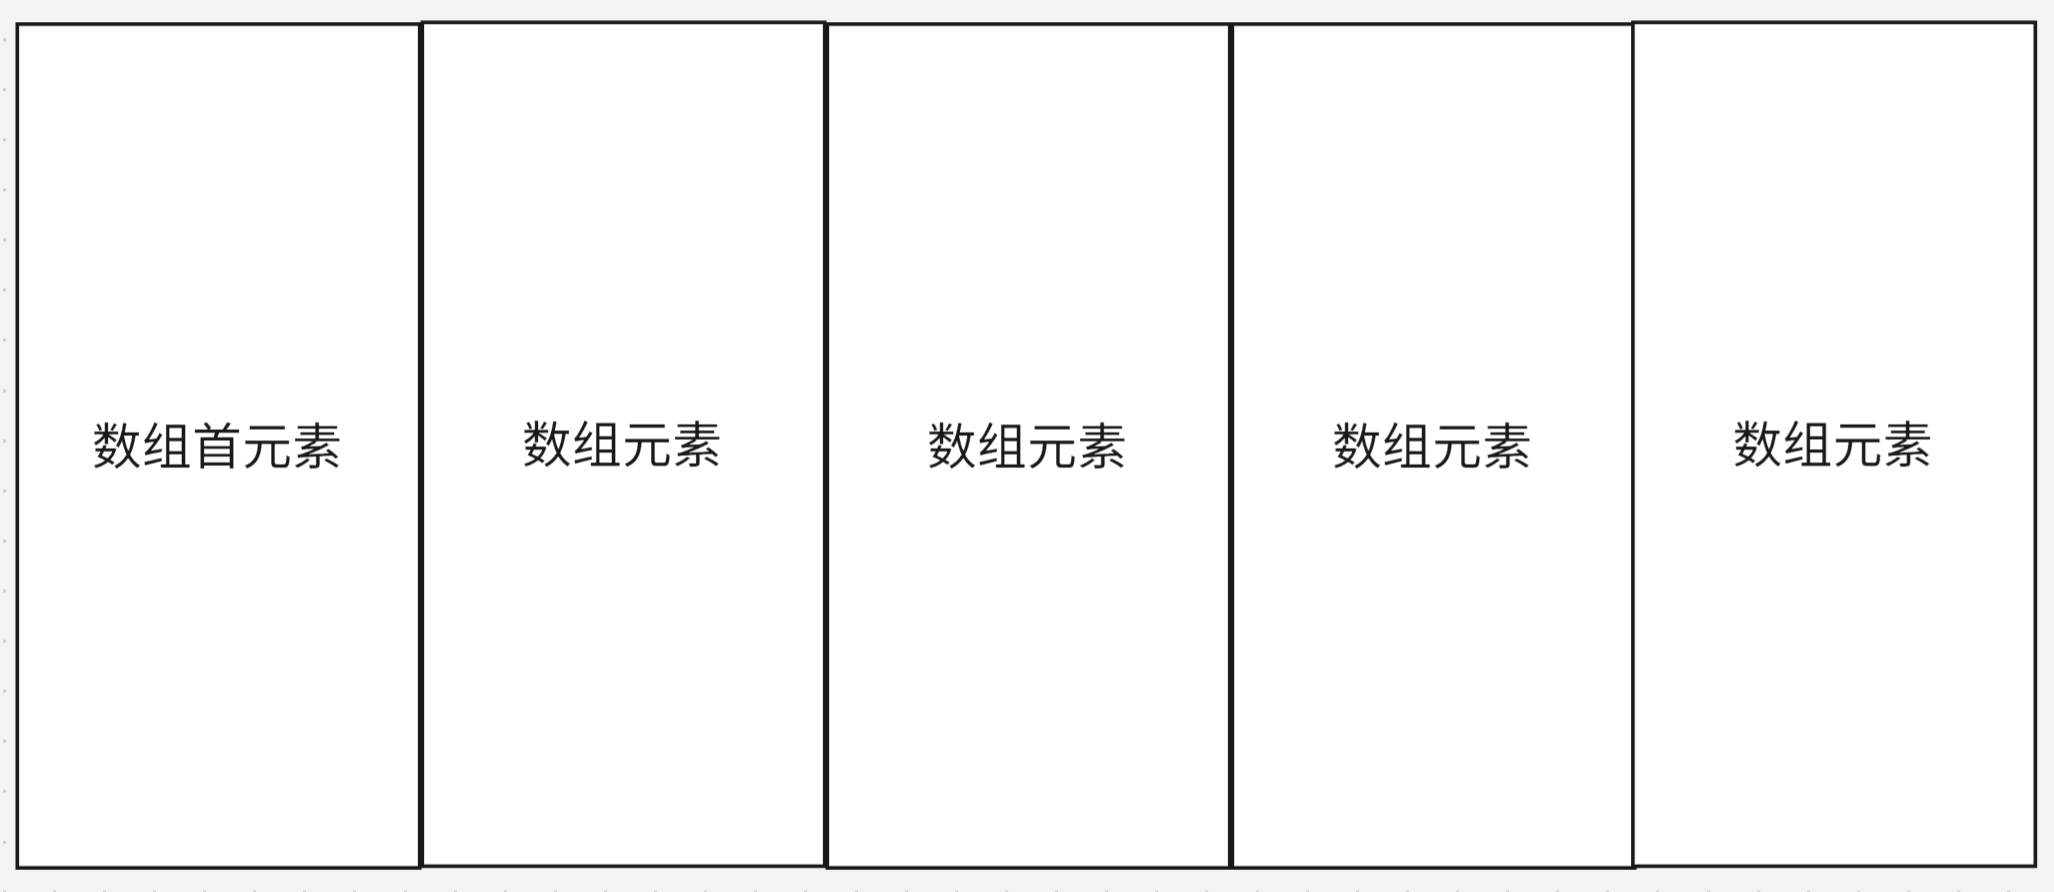
\includegraphics[width=0.7\textwidth]{数组.png}
    \caption{数组} % 图片标题
    \label{fig:数组} % 图片标签，用于引用
\end{figure}

\textbf{数组（Array）}，又称\textbf{顺序表}，它的STL容器有两种，分别是$array$和$vector$。

$array$是固定大小的数组。$vector$是一种动态数组，可以动态增长，可以根据需要自动分配内存。两者的声明方式如下：
\begin{tcode}
std::array<int,5> arr;
std::vector<int> vec;
\end{tcode}

$array$并不常用，因为它是固定大小的，如果需要改变大小，只能重新声明一个新的数组。

\begin{note}
想详细了解 \texttt{array} 可以参考这篇 blog：

\url{https://blog.csdn.net/qq_38410730/article/details/102802239}
\end{note}

$vector$由于其动态性，可以根据需要自动分配内存，因此使用起来比较方便，在工程实践中也更常用。
$vector$的实现原理是当检测到$vector$的容量不足时，会自动分配新的内存（原来的大小$\times$2），并将原有数据复制到新内存中。
这个复制的过程非常缓慢，因此，在使用大型的资源时，$vector$的效率可能会比较低。

\begin{example}
\texttt{vector} 的常用成员函数：
\begin{tcode}
#include <vector>

std::vector<int> vec{1,2,3,4,5,6};
vec[0];         //访问（快速）
vec.at(0);      //访问（安全，越界会抛异常）
vec.front();    //第一个元素
vec.back();     //最后一个元素
vec.empty();    //检查是否为空
vec.size();     //返回容器大小
vec.reserve(10);//预留空间，避免反复扩容
vec.clear();    //清除所有元素
vec.insert(vec.begin(),1);//插入元素
vec.erase(vec.begin());//删除元素
vec.push_back(1); //在最后添加
vec.emplace_back(); //在最后原位构造，省去一次拷贝
vec.pop_back();     //删除最后一个
\end{tcode}
\end{example}

\textbf{链表。}

链表是一种非连续的内存块，它是由一系列节点组成，每个节点都包含数据和指针。
链表的实现原理是每个节点都包含一个指针，指向下一个节点。链表的头节点称为头指针，尾节点称为尾指针。
链表的插入、删除操作都比较容易，只需要改变指针即可，但是查找操作比较麻烦，需要从头节点开始遍历。

\begin{note}
理论上链表的插入删除是 $O(1)$、数组的中间插入是 $O(n)$，但实际工程中链表经常\textbf{跑不过} vector：
链表的节点分散在内存各处，CPU 缓存（Cache）帮不上忙，每次访问都可能发生缓存未命中；
而 vector 的内存是连续的，缓存预取非常友好。所以除非有频繁的中部插入删除，否则默认选 vector。
\end{note}
\begin{figure}[H]
    \centering
    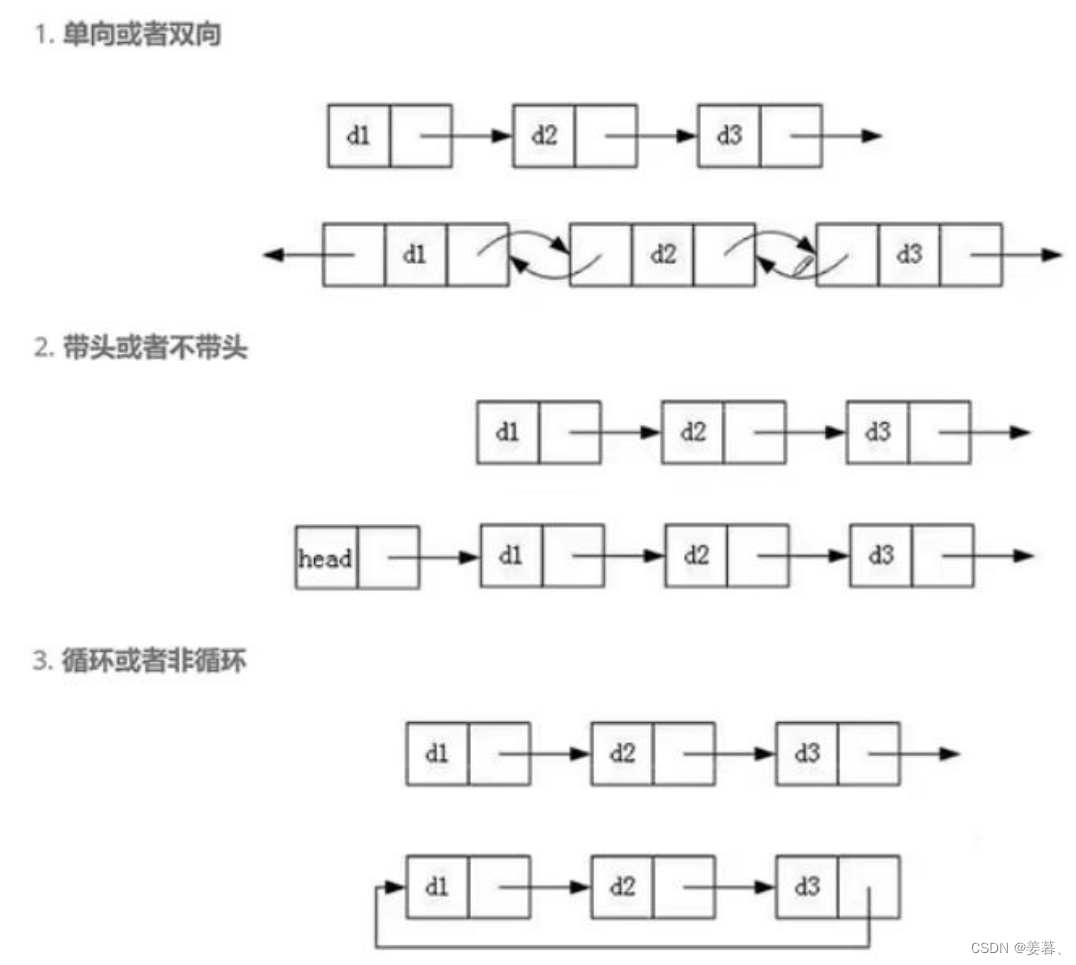
\includegraphics[width=0.7\textwidth]{链表1.png}
    \caption{链表} % 图片标题
    \label{fig:链表} % 图片标签，用于引用
\end{figure}

它的STL容器是$list$（双向链表）和$forward\_list$（单向链表）。比较简单，请自行查阅相关文档：

\url{https://zh.cppreference.com/w/cpp/container/list}

\begin{exercise}
向 \texttt{std::vector<int>} 中依次 \texttt{push\_back} 数字 $1 \sim 10$，在每次插入后打印 \texttt{size()} 和 \texttt{capacity()}，
观察容量翻倍的时机，验证"容量不足时扩容为原来 2 倍"的说法。
\end{exercise}

\subsubsection{队列、优先队列与堆栈}
\textbf{队列。}

队列是一种线性数据结构，它按照\textbf{先进先出}的原则进行操作。队列有两个基本操作，分别是\textbf{入队}和\textbf{出队}。入队操作是在队列的末尾添加一个元素，而出队操作是从队列的头部移除一个元素。队列有两个端点，队头和队尾，队头是队列的第一个元素，出队操作发生的地方，队尾是队列的最后一个元素，入队操作发生的地方。通常情况下，\textbf{不允许随机访问}队列中的元素，只能访问队头元素。
队列在\textbf{多任务处理、打印任务管理、缓冲处理}等场景中有广泛应用，它帮助维持操作的顺序和流程控制。
（很常用）
\begin{figure}[H]
    \centering
    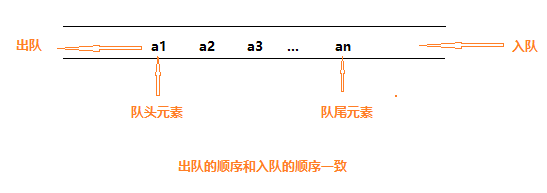
\includegraphics[width=0.7\textwidth]{队列1.png}
    \caption{入队和出队操作} % 图片标题
    \label{fig:入队和出队操作} % 图片标签，用于引用
\end{figure}
\begin{figure}[H]
    \centering
    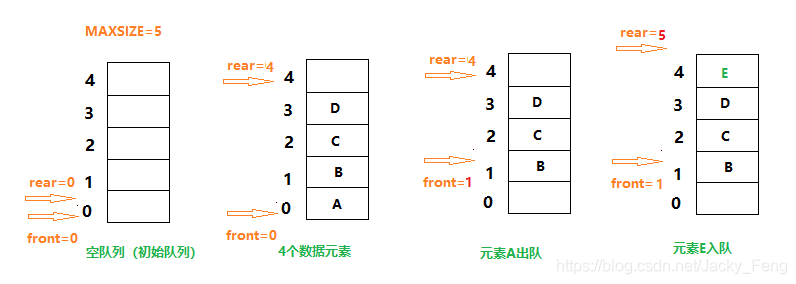
\includegraphics[width=0.7\textwidth]{队列2.png}
    \caption{队列实现方式} % 图片标题
    \label{fig:队列实现方式} % 图片标签，用于引用
\end{figure}

它的STL容器是$deque$，基于双向队列，C++还实现了3种容器适配器：
$stack$（堆栈）、$queue$（单向队列）、$priority\_queue$（优先队列）。相较于$deque$，我们更常用$queue$
进行队列操作。

\begin{note}
具体用法请自行查阅相关文档：

\url{https://zh.cppreference.com/w/cpp/container/deque}

\url{https://zh.cppreference.com/w/cpp/container/queue}
\end{note}

\textbf{优先队列。}

优先队列是一种特殊的队列，它允许插队的出现，可以根据“重要性”对队中元素进行排序。
优先队列的实现原理是每个元素都有一个优先级，优先级越高，元素越容易被取出。
优先队列的应用场景有很多，如任务调度、排序、搜索等。

\begin{figure}[H]
    \centering
    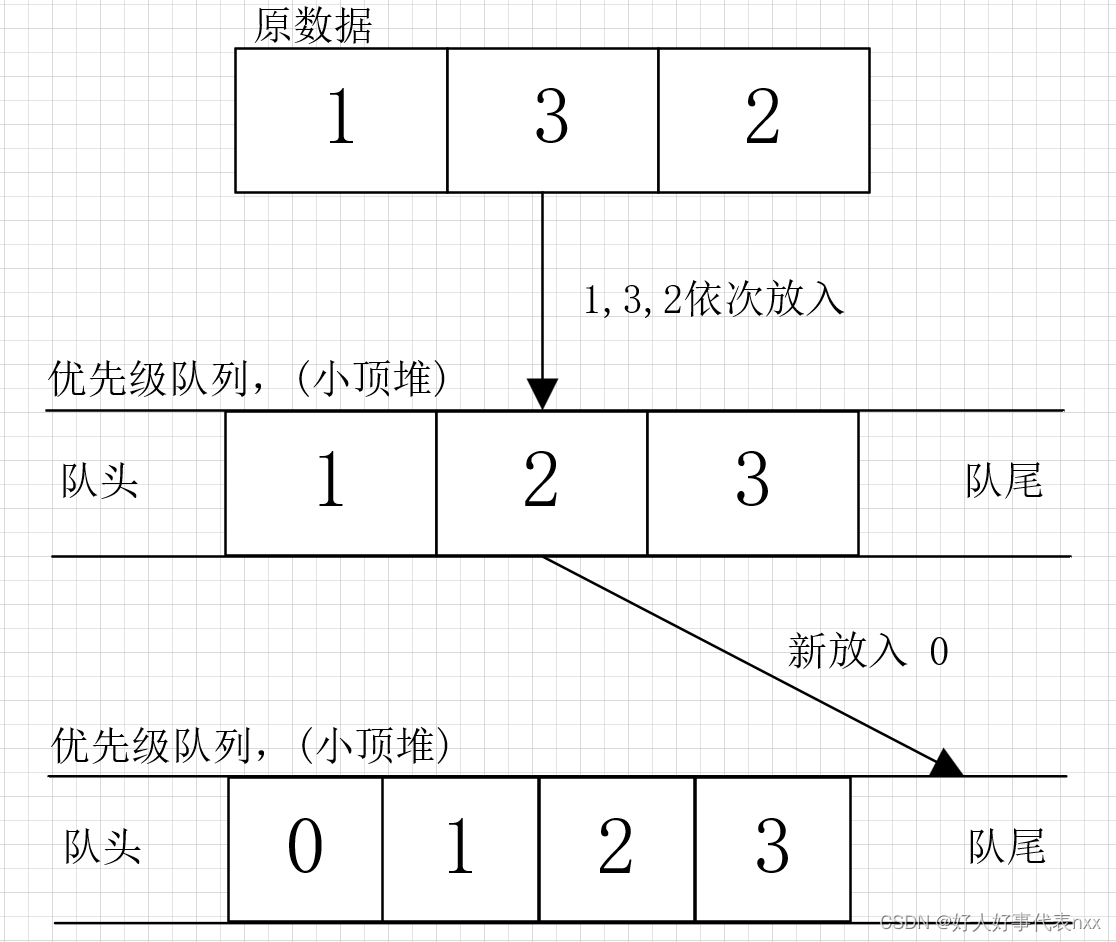
\includegraphics[width=0.7\textwidth]{优先队列1.png}
    \caption{优先队列} % 图片标题
    \label{fig:优先队列} % 图片标签，用于引用
\end{figure}

它的实现是容器适配器$priority\_queue$，
具体用法请自行查阅相关文档：

\url{https://zh.cppreference.com/w/cpp/container/priority_queue}

\textbf{堆栈。}

堆栈是一种线性数据结构，它按照\textbf{先进后出}的原则进行操作。堆栈有两个基本操作，分别是\textbf{压栈}和\textbf{弹栈}。压栈操作是在堆栈的顶部添加一个元素，而弹栈操作是从堆栈的顶部移除一个元素。堆栈有两个端点，栈顶和栈底，栈顶是堆栈的顶部，压栈操作发生的地方，栈底是堆栈的底部，弹栈操作发生的地方。
堆栈在\textbf{函数调用、表达式求值、回溯、计算器、括号匹配、迷宫寻路}等场景中有广泛应用。

\begin{figure}[H]
    \centering
    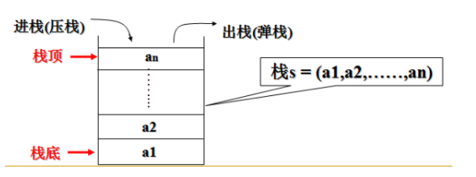
\includegraphics[width=0.7\textwidth]{堆栈1.png}
    \caption{压栈和弹栈操作} % 图片标题
    \label{fig:压栈和弹栈操作} % 图片标签，用于引用
\end{figure}
\begin{figure}[H]
    \centering
    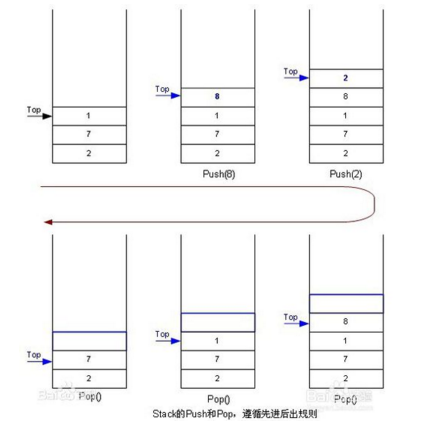
\includegraphics[width=0.7\textwidth]{堆栈2.png}
    \caption{堆栈实现方式} % 图片标题
    \label{fig:堆栈实现方式} % 图片标签，用于引用
\end{figure}

它的实现是容器适配器$stack$，
具体用法请自行查阅相关文档：

\url{https://zh.cppreference.com/w/cpp/container/stack}

\begin{exercise}
使用 \texttt{std::stack<char>} 编写括号匹配检查：读入一串只含 \texttt{(}、\texttt{)} 的字符串，
判断括号是否配对（提示：遇左括号压栈，遇右括号弹栈，弹空或结束时栈非空则不匹配）。
\end{exercise}

\subsubsection{树与堆}
\textbf{树。}

树是一种非线性数据结构，由若干\textbf{节点（Node）}和连接节点的\textbf{边（Edge）}组成。
它有且仅有一个根节点（Root），其余每个节点都恰好有一个父节点，从根节点出发可以到达任意节点，
且任意两个节点之间有且仅有一条路径——也就是说，树里不存在环路。

树还有一个更本质的\textbf{递归定义}：一棵树要么是空树；要么由一个根节点和若干棵互不相交的子树组成，
而每棵子树本身也是一棵树。"树的每个部分还是树"——正是这种自相似的结构，
让递归成为处理树最自然的方式（遍历、求高度、搜索都一行递归搞定）。

树的种类很多，如二叉树、二叉搜索树、AVL树、红黑树、B树、B+树、B*树等。
\begin{figure}[H]
    \centering
    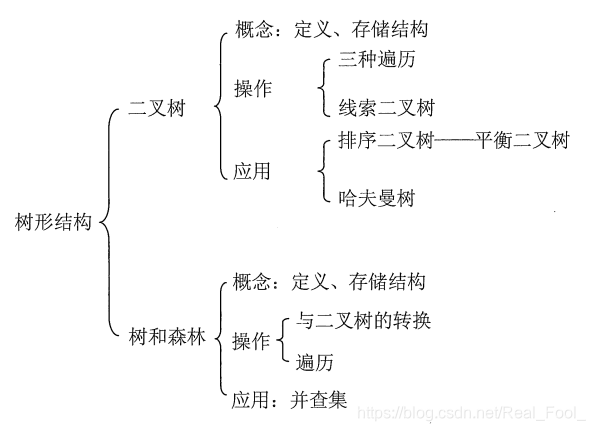
\includegraphics[width=0.7\textwidth]{树1.png}
    \caption{树的逻辑图（了解即可）} % 图片标题
    \label{fig:树的逻辑图} % 图片标签，用于引用
\end{figure}

\begin{figure}[H]
    \centering
    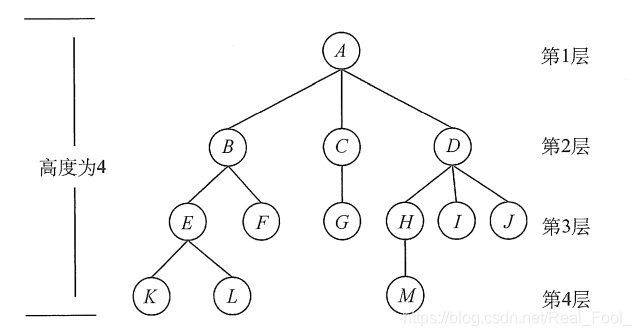
\includegraphics[width=0.7\textwidth]{树2.png}
    \caption{树的示意图} % 图片标题
    \label{fig:树的示意图} % 图片标签，用于引用
\end{figure}

\textbf{堆。}

堆是一种特殊的树，它是一个\textbf{完全二叉树}，即除叶节点外，其他的每个节点都有两个子节点。
每个节点都有一个值，并且每个节点\textbf{都大于或等于其子节点}（这是最大堆max-heap，类似的，还有最小堆min-heap）。堆的应用场景有很多，如排序、优先队列、图算法、堆排序等。

\begin{figure}[H]
    \centering
    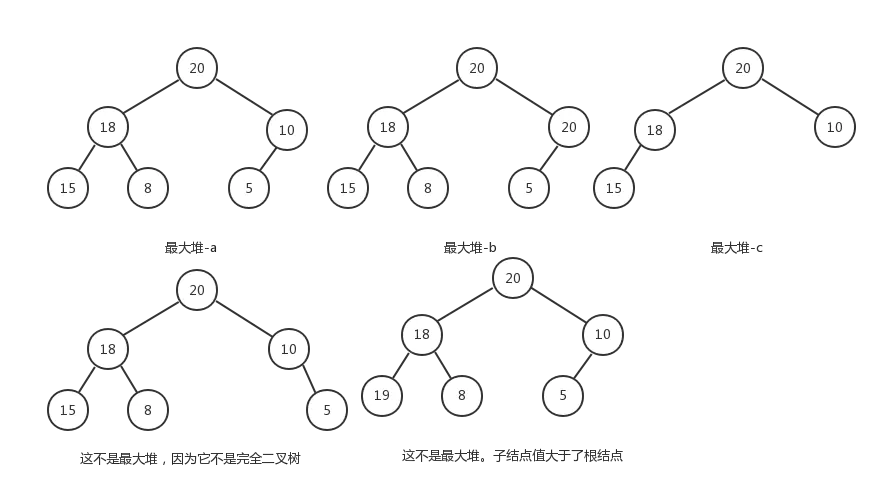
\includegraphics[width=0.7\textwidth]{最大堆.png}
    \caption{最大堆的示意图} % 图片标题
    \label{fig:最大堆} % 图片标签，用于引用
\end{figure}

\begin{figure}[H]
    \centering
    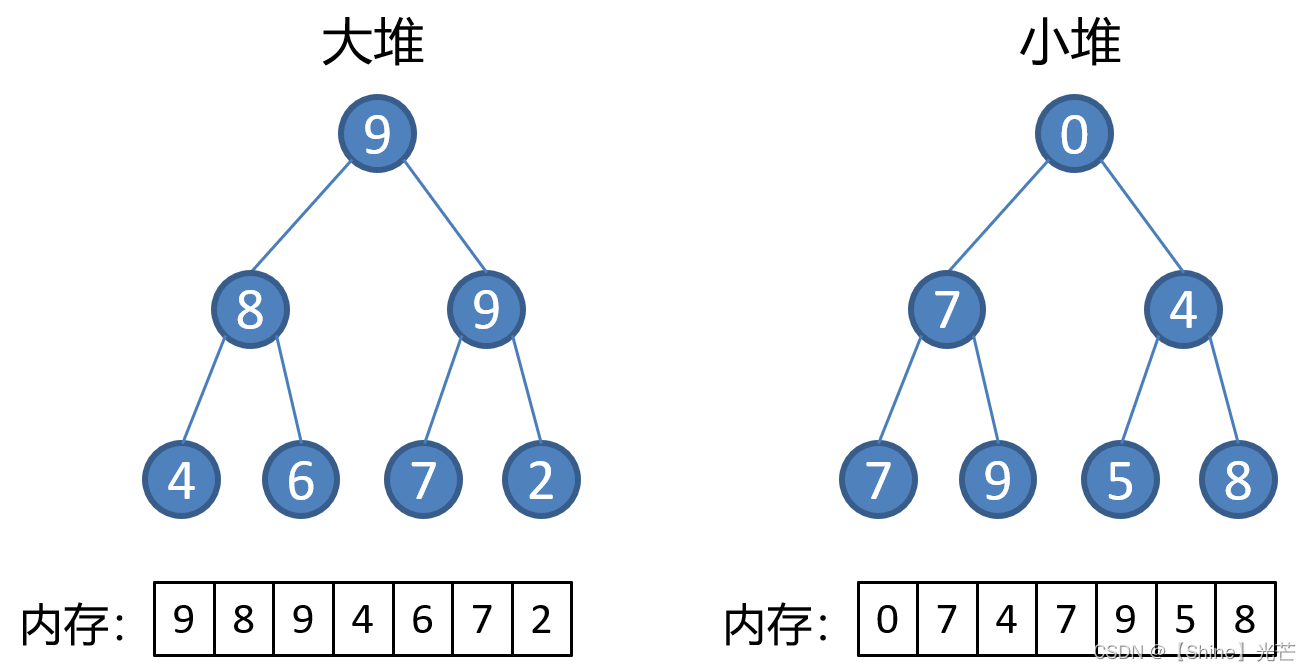
\includegraphics[width=0.7\textwidth]{堆1.png}
    \caption{最大堆和最小堆} % 图片标题
    \label{fig:最大堆和最小堆} % 图片标签，用于引用
\end{figure}

上一小节介绍的优先队列正是基于堆实现的：它通过为每个任务的重要程度编号，把编号大的任务放在堆顶，
从而快速取出最重要的任务；堆的调整算法很快，因此优先队列被广泛应用于\textbf{任务管理}中。
优先队列的容器用法已在上一小节给出，这里不再重复。

\subsubsection{映射}

映射是一种关联容器，它是一个\textbf{键值对}的集合，其中每个键都是唯一的，值可以重复。
映射有两种主流实现：基于哈希表的实现查找、插入、删除的平均时间复杂度是$O(1)$；
基于红黑树的实现则是$O(logN)$，但能保持键有序。

\textbf{红黑树（Red-Black Tree）}是一种随机查找速度比较快的\textbf{平衡二叉树}\footnote{
    平衡二叉树，也叫AVL树，它或者是一棵空树，或者具有以下性质的二叉排序树：它的左子树和右子树的高度之差（平衡因子）的绝对值不超过1，且它的左子树和右子树都是一棵平衡二叉树}
，它的查找、插入、删除操作的时间复杂度都是$O(logN)$\footnote{
    O(logN)表示时间复杂度，N是问题的规模，O表示运行消耗时间的上界
}。

\textbf{哈希表（HashTable）}是一种\textbf{散列表}，它通过\textbf{哈希函数}将键映射到值。
由于其使用计算来查找，因此，查找操作的平均时间复杂度是$O(1)$
\footnote{常数的时间复杂度意味着不管问题的规模如何，
对于同一个长度的HashTable，算法的运行时间都不会随着问题的规模增加而增长。}。
但是哈希表的建立比较困难，需要消耗很多资源。
而且存储长度有限，当元素过多时，哈希表的性能会下降。当哈希表满时，需要执行\textbf{再散列（Rehashing）}，解决\textbf{哈希冲突（Hash Collision）}问题，
这个过程需要消耗大量时间。

两者各有优劣，在实际应用中，需要根据具体问题选择。
红黑树型映射的STL容器是$map$，哈希表型映射的STL容器是$unordered\_map$。

\begin{example}
\texttt{map} 与 \texttt{unordered\_map} 的基本用法：
\begin{tcode}
#include <iostream>
#include <map>
#include <unordered_map>
#include <string>

int main() {
    std::map<std::string,int> score;            //红黑树实现，按键有序
    score["alice"] = 90;                        //插入或修改
    score.emplace("bob", 85);
    std::cout << score["alice"] << std::endl;   //按键访问
    std::cout << score.count("carol") << std::endl; //判断键是否存在：0
    for(auto& [name, s] : score){               //遍历，按字母序输出
        std::cout << name << ": " << s << std::endl;
    }

    std::unordered_map<std::string,int> fastScore; //哈希表实现，无序但更快
    fastScore["alice"] = 90;
    return 0;
}
\end{tcode}
\end{example}

\begin{note}
具体用法请自行查阅相关文档：

\url{https://zh.cppreference.com/w/cpp/container/map}

注意：\texttt{map} 的 \texttt{operator[]} 在键不存在时会\textbf{自动插入}一个默认值，
只想查询不想改动时，请用 \texttt{find()} 或 \texttt{count()}。
\end{note}

\begin{exercise}
使用 \texttt{std::map<std::string,int>} 统计一段文字中每个单词出现的次数，并按键的字母序打印结果。
\end{exercise}

\subsubsection{迭代器与失效}

迭代器是一种检查容器内元素并遍历元素的数据类型，通常用于对C++中各种容器内元素的访问，
但不同的容器有不同的迭代器，初学者可以将迭代器理解为一个可以\textbf{自动向后移动的指针}。

常用的可迭代的容器有：

\begin{enumerate}
    \item 序列容器：$array$、$vector$、$deque$、$list$、$forward\_list$等
    \item 关联容器：$set$、$map$、$multimap$等
\end{enumerate}

$queue$、$stack$、$priority\_queue$是容器适配器，必须满足一定规则，没有迭代器。

对于可迭代容器，一般可以使用.begin()和.end()方法获取迭代器，.begin()方法返回指向第一个元素的迭代器，
.end()方法返回指向最\textbf{后一个元素的迭代器的下一位置}。

\begin{example}
用迭代器遍历容器：
\begin{tcode}
#include <iostream>
#include <vector>

int main() {
    std::vector<int> vec{1,2,3,4,5,6,7,8,9,0};
    for(auto it = vec.begin();it != vec.end();++it){
        std::cout << *it << std::endl;
    }
    return 0;
}
\end{tcode}
\end{example}

也可以简写为范围for循环：

\begin{tcode}
for (auto it : vec) {
    std::cout << it << std::endl;
}
\end{tcode}

\begin{example}
迭代器的常见修改操作：
\begin{tcode}
#include <algorithm> //sort、remove_if、iter_swap 都在这个头文件里

std::vector<int> vec{1, 2, 3, 4, 5, 6, 7, 8, 9, 0};
vec.erase(vec.begin()+5);            //删除第6个元素
vec.erase(vec.begin()+5, vec.end()); //删除第6个元素之后的所有

std::vector<int> vec1{1, 2, 3, 4, 5, 6, 7, 8, 9, 0};
std::iter_swap(vec1.begin(), vec1.begin()+1); //交换第一个和第二个元素

std::vector<int> vec2{1, 2, 3, 4, 5, 6, 7, 8, 9, 0};
std::sort(vec2.begin(), vec2.end(), [](int a, int b){
    return a >= b;                  //降序排序
});

//remove_if 只把不满足条件的元素挪到前面，并不真正删除
//正确姿势是 erase-remove 惯用法：
vec2.erase(std::remove_if(vec2.begin(), vec2.end(), [](int a){
    return a > 5;
}), vec2.end());                    //这才真正删除了大于5的元素
\end{tcode}
\end{example}

\begin{note}
\texttt{std::remove\_if} 并不会改变容器大小，它只是把"要保留"的元素搬到前面、返回新的逻辑结尾迭代器，
必须配合 \texttt{erase} 才能完成删除——这就是著名的 erase-remove 惯用法。忘记接 \texttt{erase}，
容器里会留下一堆"僵尸元素"。更多迭代器内容见 cppreference：

\url{https://zh.cppreference.com/w/cpp/iterator}
\end{note}

\textbf{迭代器失效。}

迭代器失效指的是迭代器因为某些操作而不再指向原来的元素，
或者不再保持有效的状态，这样的迭代器如果继续使用，可能会导致未定义行为，包括程序崩溃。
通俗的理解就是，当你对容器进行了操作时，更改了容器的大小，但是迭代器仍然指向原来的位置，
这样就会导致读取错误的内存，这就是迭代器失效。

\begin{tcode}
std::vector<int> vec={1,2,3,4,5,6,7,8,9,10};
for(auto it = vec.begin(); it != vec.end(); ++it){
    if(*it % 2 == 0){
        vec.erase(it); //错误示范：erase之后it已经失效
    }
}
\end{tcode}

看上面的代码，当执行到vec.erase(it)时，it已经失效，因为执行了erase之后，
vec的大小发生了变化，这导致了迭代器失效。

在实践过程中，下面的几种情况下迭代器会失效，需要\textbf{避免}出现：
\begin{enumerate}
    \item 当执行erase方法时，指向删除节点的迭代器失效，指向删除节点之后的迭代器也全部失效
    \item 当进行push\_back()方法时，end操作返回的迭代器肯定失效
    \item 当插入（push\_back）一个元素后，capacity返回值与插入之前相比有改变，
    则说明容器整体搬了家，此时所有迭代器都会失效
    \item 当插入（push\_back）一个元素后，如果空间未重新分配，指向插入位置之前的元素的迭代器仍然有效，但指向插入位置之后元素的迭代器全部失效
\end{enumerate}

对于关联容器，删除一个键值对只会使当前这个迭代器失效，别的迭代器不会受到影响，
这可能是由于底层使用红黑树实现的原因。但是实际应用中，仍然不应该冒这个风险，因此，
必须\textbf{坚决避免迭代器失效问题的发生}。

在具体的应用中，我们在使用迭代器遍历时，应该注意不要对容器进行增删操作，更不应该改变容器的大小。
正确的删除写法是利用 erase 的返回值——它会返回指向被删元素\textbf{下一个}元素的有效迭代器：

\begin{example}
遍历中安全删除元素：
\begin{tcode}
std::vector<int> vec={1,2,3,4,5,6,7,8,9,10};
for(auto it = vec.begin(); it != vec.end(); ){ //注意：这里没有++it
    if(*it % 2 == 0){
        it = vec.erase(it); //erase返回下一个有效迭代器
    }else{
        ++it;
    }
}
\end{tcode}
\end{example}

\begin{conclusion}
迭代器失效自救指南：

\begin{itemize}
\item 遍历容器时不要随手增删元素，先想清楚迭代器下一步指向哪；
\item 删除元素用 \texttt{it = vec.erase(it);} 接住返回值，而不是 \texttt{vec.erase(it);} 后继续用旧迭代器；
\item push\_back 导致扩容后，之前保存的所有迭代器、指针、引用全部作废，需要遍历就重新获取；
\item 批量按条件删除，优先考虑 erase-remove 惯用法，一行解决，不容易写错。
\end{itemize}
\end{conclusion}

\begin{exercise}
把"错误示范"的代码抄下来运行，观察运行结果或崩溃现象；再用"遍历中安全删除元素"的写法修复它，
删除所有偶数并打印剩余的奇数。
\end{exercise}


\section{C++ 多线程}
本节展开多线程同步与常见模型，并将系统内存布局作为相关基础一并说明。

\subsubsection{基本概念}
多线程技术是C++中非常重要的特性之一，它可以让程序员以更高的并发性和速度运行程序。使用多线程可以提高程序的运行效率，丰富程序的运行逻辑，实现许多单线程所不能实现的功能。
在C++中，提供了$<thread>$库来实现多线程的功能。

\textbf{多线程的原理}：多线程是指在同一程序中同时运行多个线程来完成不同的任务，以提高资源利用率和程序响应速度。
硬件条件上，多线程需要CPU支持多核处理或多任务处理，以及足够的内存和处理器资源。在多线程编程过程中，可能遇到一些问题，
包括线程同步、死锁、竞态条件等，这些问题可能导致程序运行不稳定、性能下降甚至系统崩溃。
因此，在设计多线程程序时，需要充分考虑线程之间的\textbf{协作与互斥}，合理分配资源，以保障程序的正确性和高效性。
在多线程之中，有两种主要的设计模式，即\textbf{阻塞}和\textbf{非阻塞}。

\begin{enumerate}
    \item \textbf{阻塞}：在阻塞模式下，线程在等待某个事件的发生，如等待IO操作完成、等待子进程结束等。
当某个事件发生时，线程会被唤醒，并开始执行。

    \item \textbf{非阻塞}：在非阻塞模式下，线程在等待某个事件的发生，但不会被挂起，而是继续执行后续代码。
当某个事件发生时，线程会被通知，并开始执行。
\end{enumerate}


\subsubsection{创建与生命周期}
C++11中引入的$<thread>$库提供了多线程的支持，它提供了$std::thread$类来创建和管理线程:

\begin{tcode}
用法：std::thread ThreadName(函数指针，[参数]);
实例：
void function1(){for(int i=0;i<1000;i++);}
void function2(int a,int &b){for(int i=0;i<1000;i++);}
int main() {
    std::thread th1(function1);
    int a=0, b=0;
    std::thread th1(function1,a,std::ref(b));
    return 0;
}
\end{tcode}

如果你想要在线程中传递参数，可以直接传递参数，也可以使用引用传递参数，引用传参的时候需要使用$std::ref()$函数。
你也可以使用$join()$方法使主线程等待所有线程结束，
$detach()$方法将线程分离，这样主线程就不会等待主线程结束而结束。

\subsubsection{互斥与锁}
多线程程序的稳定性和互斥锁是多线程编程中经常遇到的问题。请参考下面的例子：
\begin{tcode}
int i=0;
void function1(){
    for(int j=0;j<100000;j++)
        i++;
}

int main() {
    std::thread th1(function1);
    for(int j=0;j<100000;j++)
        i++;
    if(th1.joinable())
        th1.join();
    std::cout << i;
    return 0;
}
\end{tcode}
在程序的运行过程中，$i$的值可能是$0$，也可能是$200000$，这取决于线程的调度。
当两个线程同时拿到$i$的地址时，同时对i进行写入操作，两者就会出现线程同步问题。
那怎么解决这个问题呢？$std::mutex$和$std::lock\_guard$为我们提供了解决方案——互斥锁。是解决线程同步问题的两种方法。
$mutex$是一种同步机制，它可以保证同一时刻只有一个线程对共享资源进行访问。
$lock\_guard$是一个智能指针，它可以自动获取互斥锁，并在离开作用域时自动释放互斥锁。

\begin{tcode}
#include <iostream>
#include <thread>
#include <mutex>

int i=0;
std::mutex lock;
void function1(){
    for(int j=0;j<100000;j++){
        lock.lock();
        i++;
        lock.unlock();
    }
}

int main() {
    std::thread th1(function1);
    for(int j=0;j<100000;j++){
        lock.lock();
        i++;
        lock.unlock();
    }
    if(th1.joinable())
        th1.join();
    std::cout << i;
    return 0;
}
\end{tcode}
发现程序的稳定性已经得到提高，在多次运行过程中，$i$的值始终是$200000$。这一点在多线程编程过程中非常重要，是所有程序员的必修课。
但是，这是又产生了一个新的问题，那就是程序员还是需要进行互斥锁的手动管理，这无疑会降低程序开发的效率。
类似于智能指针的，C++11中引入了$std::lock\_guard$来自动管理互斥锁，它可以自动获取互斥锁，并在离开作用域时自动释放互斥锁。

\begin{tcode}
#include <iostream>
#include <thread>
#include <mutex>

int i=0;
std::mutex lock;
void function1(){
    for(int j=0;j<100000;j++){
        std::unique_lock<std::mutex> Autolock;
        i++;
    }

}

int main() {
    std::thread th1(function1);
    for(int j=0;j<100000;j++){
        std::unique_lock<std::mutex> Autolock;
        i++;
    }

    if(th1.joinable())
        th1.join();
    std::cout << i;
    return 0;
}
\end{tcode}
程序测试成功，$i$的值始终是$200000$。

\subsubsection{死锁}
在使用互斥锁的时候，如果多个线程都在\textbf{等待对方释放锁}，就会出现死锁。请看下面的例子：

\begin{tcode}
int i=0;
std::mutex lock1;
std::mutex lock2;
void function1(){
    for(int j=0;j<100000;j++){
        lock1.lock();
        lock2.lock();
        i++;
        lock2.unlock();
        lock1.unlock();
    }
}

int main() {
    std::thread th1(function1);
    for(int j=0;j<100000;j++){
        lock2.lock();
        lock1.lock();
        i++;
        lock2.unlock();
        lock1.unlock();
    }

    if(th1.joinable())
        th1.join();
    std::cout << i;
    return 0;
}

\end{tcode}

在这个例子中，两个线程都在等待对方释放锁，导致死锁。在设计时，尽量使得不同的互斥锁以相同的顺序被获取和释放，可以降低死锁的概率。

\subsubsection{原子变量与条件变量}
\textbf{原子变量。}
在C++11中，引入了原子类型$std::atomic$，它可以保证变量的原子性，即在读写操作时，其他线程只能看到该变量的\textbf{已修改}值。
使用这种方式，可以增强程序的可读性。原子变量也不需要使用互斥锁进行同步，它可以自动保证原子性。

\textbf{条件变量。}条件变量通常与互斥锁配合使用，使一个线程在另一线程满足特定条件后再继续执行。

条件变量使线程在共享状态满足特定条件后再继续执行，从而避免忙等待。

使用条件变量主要是因为它们提供了在多线程编程中一种有效的同步机制。
当多个线程需要\textbf{等待某个特定条件}成立才能继续执行时，条件变量就显得尤为重要。
通过条件变量，线程可以安全地进入等待状态，直到被其他线程显式地唤醒或满足等待的条件。
这有助于避免线程的\textbf{无谓轮询或忙等待}，提高了系统的响应能力和效率。
\textbf{注意}：在使用条件变量时，必须确保与\textbf{互斥锁}一起使用，以\textbf{避免竞态条件}的发生。

下面介绍一下$condition\_variable$的用法：

条件变量的使用大致可以分为两个大的功能，即$notify$和$wait$。

\begin{tcode}
std::condition_variable condition;//声明
condition.notify_all();//通知所有等待线程
condition.notify_one();//通知第一个接收的等待线程

std::unique_lock<std::mutex> Lock(mtx);
condition.wait(Lock);//等待条件成立
condition.wait(Lock,[](){return true;});//等待条件和第二个参数同时为true
\end{tcode}

\subsubsection{生产者—消费者与线程池}
\textbf{生产者—消费者模型。}
生产者-消费者模型是指多个生产者线程和多个消费者线程之间通过一个共享的缓冲区进行通信。
生产者线程负责生产数据，并将其放入缓冲区；消费者线程则负责从缓冲区中取出数据进行消费。
生产者和消费者之间通过一个\textbf{条件变量}进行同步，以保证缓冲区中的数据不会被消费者线程消费完。

\begin{tcode}
#include<iostream>
#include<thread>
#include<mutex>
#include<condition_variable>
#include<queue>
#include<functional>

std::mutex lock;
std::condition_variable cv;
std::queue<std::function<void()>> taskQueue;
void consumer(){
    while(1){
        std::unique_lock<std::mutex> Lock(lock);
        cv.wait(Lock,[&](){
            return !taskQueue.empty();
        });
        auto task = taskQueue.front();
        task();
        taskQueue.pop();
        Lock.unlock();
    }
}

void producer(int i){
    auto func = [](int id){
        std::cout << "task" << id << " is running!" << std::endl;
    };
    std::function<void()> task = std::bind(func,i);
    {
        std::unique_lock<std::mutex> Lock(lock);
        taskQueue.push(task);
    }
    cv.notify_one();
    std::this_thread::sleep_for(std::chrono::seconds(1));
}

int main(int argc,char** argv){
    std::thread consumer_thread(consumer);
    for(int i=0;i<100;i++){
        producer(i);
    }

    if(consumer_thread.joinable())
        consumer_thread.join();
    return 0;
}
\end{tcode}

\textbf{线程池。}
线程池是一种常用的技术，它可以提高程序的并发性，减少线程创建和销毁的开销，并可以有效的利用系统资源。
下面是一种线程池的实现方式，尝试一下把它看懂吧！

\begin{tcode}
#include <iostream>
#include <thread>
#include <mutex>
#include <condition_variable>
#include <functional>
#include <vector>
#include <queue>

class ThreadPool
{
private:
    std::vector<std::thread> threads;
    std::queue<std::function<void()>> tasks;
    std::mutex mtx;
    std::condition_variable condition;
    bool stop;

public:
    ThreadPool(int numThreads):stop(false) {
        for (int i = 0; i < numThreads; i++) {
            threads.emplace_back([this] {
                while (1) {
                    std::unique_lock<std::mutex> lock(mtx);
                    condition.wait(lock, [this] {
                        return !threads.empty() || stop;
                    });
                    if (stop && tasks.empty())
                        return;

                    auto task = std::move(tasks.front());
                    tasks.pop();
                    lock.unlock();
                    task();
                }
            });
        }

    }

    ~ThreadPool() {
        {
            std::unique_lock<std::mutex> lock(mtx);
            stop = true;
        }
        condition.notify_all();
        for (auto& iter : threads) {
            iter.join();
        }
    }

    template<class F, class ...Args>
    void enqueue(F&& f, Args&&... args) {
        std::function<void()> task =
                std::bind(std::forward<F>(f), std::forward<Args>(args)...);
        {
            std::unique_lock<std::mutex> lock(mtx);
            tasks.emplace(std::move(task));
        }
        condition.notify_one();
    }

};

int main() {
    ThreadPool Pool(4);
    for (int i = 0; i < 100; i++) {
        Pool.enqueue([i] {
            std::cout << "task" << i << "is running!" << std::endl;
            std::this_thread::sleep_for(std::chrono::seconds(1));
            std::cout << "task" << i << "has finished!" << std::endl;
        });
    }

    return 0;
}

\end{tcode}

\subsubsection{并发进阶}

前述线程池属于入门实现。视觉工程中常见多传感器回调、处理线程与结果队列的组合，其本质是多生产者—多消费者问题。以下补充关键接口与用法。系统练习见 \texttt{参考文献/multithread.pdf}。

\textbf{1. \texttt{unique\_lock} 与 \texttt{condition\_variable}}

队列为空时，消费者应进入等待，而不是轮询占用 CPU。

\begin{tcode}
std::mutex mtx;
std::condition_variable cv;
std::queue<int> q;

void consumer() {
    std::unique_lock<std::mutex> lock(mtx);
    cv.wait(lock, [] { return !q.empty(); }); // 谓词用于抑制虚假唤醒
    int v = q.front(); q.pop();
}

void producer(int v) {
    {
        std::lock_guard<std::mutex> lock(mtx);
        q.push(v);
    }
    cv.notify_one();
}
\end{tcode}

\texttt{condition\_variable} 须与 \texttt{unique\_lock} 配合使用。\texttt{wait} 可能发生虚假唤醒，因此必须提供条件谓词。

\textbf{2. \texttt{packaged\_task} 与 \texttt{future}}

线程池提交任务后，调用方常需获取返回值：以 \texttt{packaged\_task} 包装可调用对象，调用 \texttt{get\_future()}，在工作线程中执行任务，最后通过 \texttt{future.get()} 取得结果。\texttt{packaged\_task} 仅可移动、不可拷贝，不能直接放入要求可拷贝的 \texttt{std::function}。

\textbf{3. \texttt{shared\_mutex}}

读多写少场景下，普通 \texttt{mutex} 会使读者相互阻塞。应使用共享锁：

\begin{tcode}
std::shared_mutex rw;
std::unordered_map<std::string, int> data;

int read(const std::string& key) {
    std::shared_lock lock(rw);
    return data.at(key);
}
void write(const std::string& key, int val) {
    std::unique_lock lock(rw);
    data[key] = val;
}
\end{tcode}

并发压力较高时，可对容器进行哈希分片，使每个分片持有独立锁，从而降低竞争。

\textbf{4. 死锁避免}

死锁需同时满足互斥、持有并等待、不可抢占与循环等待。破坏任一条件即可避免死锁。常用方法是所有线程按统一顺序获取锁；亦可使用 \texttt{std::lock} 同时获取多把锁，再以 \texttt{std::adopt\_lock} 交由 \texttt{lock\_guard} 管理释放。

\textbf{5. \texttt{atomic}、\texttt{future}、\texttt{promise} 与 \texttt{chrono}}

\begin{itemize}
    \item 简单计数与停止标志宜使用 \texttt{std::atomic}，避免为计数引入过大锁粒度。
    \item \texttt{promise} 为写端，\texttt{future} 为读端，用于跨线程传递单次结果；\texttt{std::async} 可简化异步调用。
    \item 限时等待宜使用 \texttt{condition\_variable::wait\_for}，以支持超时返回或被通知后立即结束，优于单纯的 \texttt{sleep\_for}。
\end{itemize}

\textbf{6. 综合练习}

建议以 \texttt{参考文献/multithread.pdf} 作为多线程章节的综合训练。

\begin{center}
\begin{tabular}{clp{7.2cm}}
\toprule
阶段 & 分值 & 对应能力 \\
\midrule
Phase 1 派遣大厅 & 25 & 线程安全队列与线程池：互斥、条件变量、\texttt{future}、完美转发 \\
Phase 2 档案馆 & 30 & 读写锁、分片、\texttt{atomic}、TTL 与可中断等待 \\
Phase 3 交易所 & 25 & 事务、按序加锁避免死锁、\texttt{any} \\
Phase 4 远征 & 20 & 同步接口的异步封装、批量 \texttt{future} \\
\bottomrule
\end{tabular}
\end{center}

通识阶段须至少完成 Phase~1，其余阶段可按能力选做。构建与测试可采用 CMake 与 \texttt{ctest}；排查数据竞争时可启用 ThreadSanitizer，编译选项为 \texttt{-DENABLE\_TSAN=ON}。

\subsubsection{系统级内存运行逻辑}
C++是一个十分灵活的编程语言，其中指针的概念为程序员们提供了直接操纵内存的能力。
指针的使用使得程序员可以自由的操作内存，但是也带来了一些安全性和复杂性问题。
因此，了解程序运行的底层逻辑，对于理解C++至关重要，对于提高程序效率举重若轻，下面我们来看看C++的内存运行逻辑。

\begin{figure}[H]
    \centering
    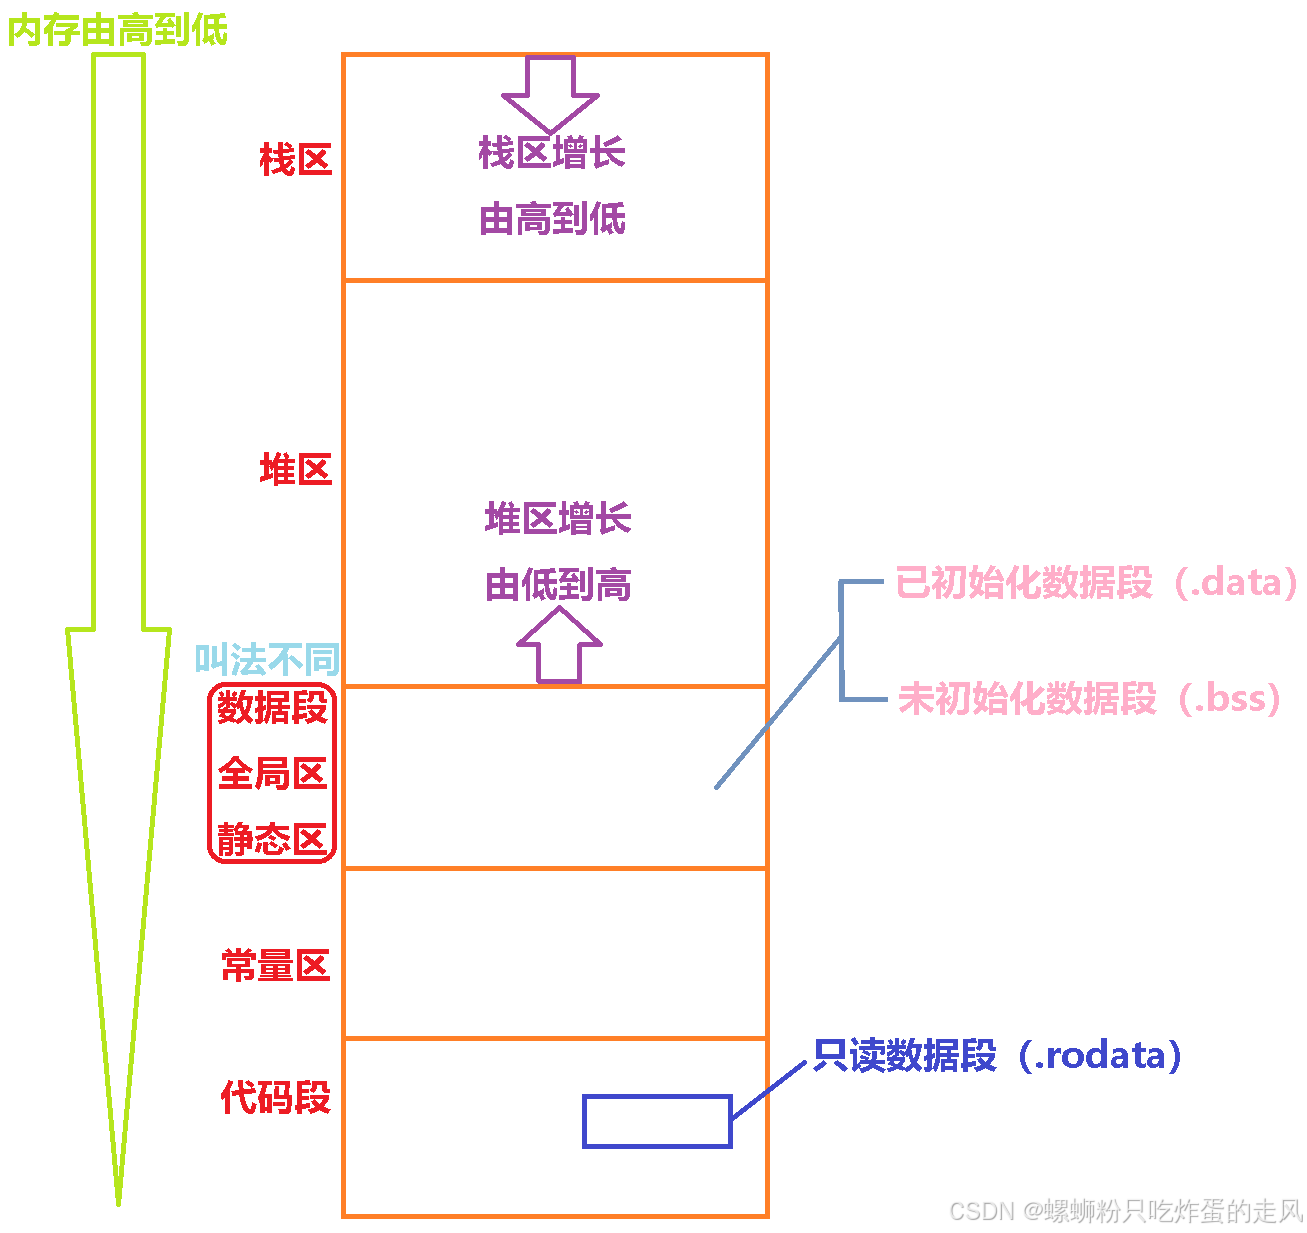
\includegraphics[width=0.7\textwidth]{系统内存.png}
    \caption{系统内存分区} % 图片标题
    \label{fig:内存分区} % 图片标签，用于引用
\end{figure}

如图\ref{fig:内存分区}，系统内存分为\textbf{代码区、常量区、全局/静态变量区、堆区、栈区等几个部分}。

\textbf{代码区和常量区}是存放程序代码和常量数据的区间一般不作区分，这里的数据是只读的，其中存储着一些在编译过程前就可以确定的数据内容
，如代码、$constexpr$修饰的变量、$const$修饰的在预编译期可以确定的值等，
一些字面常量如"Hello World!"，也存储于其中。程序在常量区中只能读取数据。

\textbf{全局/静态变量区}是存放全局/静态变量的区间，全局变量在程序运行前就已经分配了内存，静态变量在程序运行前也已经分配了内存。
但是静态变量的生命周期比全局变量长，它在程序运行结束后才释放内存。

\begin{enumerate}
    \item 全局变量：在函数外部定义的变量，它们具有全局作用域。
    \item 静态全局变量：在函数外部定义并用 $static$ 关键字修饰的变量，它们具有内部链接属性，即它们只能在定义它们的文件内部可见。
    \item 静态局部变量：在函数内部定义并用 $static$ 关键字修饰的变量，它们在函数调用结束后仍然存在，并且保持它们的值。
    \item 类静态成员变量：在类定义中使用 $static$ 关键字声明的成员变量，它们属于类而不是类的任何一个实例。
\end{enumerate}

解释一下\textbf{静态}：
\begin{enumerate}
    \item 生命周期上，静态变量在程序开始运行前或类的实例化之前就已经分配了内存，在程序运行结束后才释放内存。地址不会发生变化，就静静“躺”在静态变量区，直到程序结束。
    \item 相对于$new$的动态分配，可以让程序员选择什么时候分配和释放内存，而$static$变量则是一直存在的，直到程序结束。
    \item 静态全局变量也具有全局作用域，他与全局变量的区别在于如果程序包含多个文件的话，他作用于定义它的文件里，不能作用到其他文件里，即被$static$关键字修饰过的变量具有文件作用域。这样即使两个不同的源文件都定义了相同的静态全局变量，他们也是不同的变量。这点于全局变量不同。
\end{enumerate}

\textbf{堆区}：堆区是由程序员手动分配和释放的内存，堆区的分配和释放由\textbf{程序员控制}，程序员可以通过$new$和$delete$操作符来分配和释放内存。

在大小上，堆区的大小相对于栈区是很大的，因此可以存储更多的数据。初次之外，堆区是由程序员全权负责管理的，程序员必须小心管理堆区的分配和释放，确保程序的正确性和安全性，一般使用\textbf{智能指针}和$nullptr$判断提高程序的稳定性。
但与此同时，堆区也提供了更为灵活的编程和数据传递模式，可以参考下面的例子：
\begin{tcode}
std::vector<int>* func(){
    std::vector<int>* a = new std::vector<int>({1,2,3,4});
    std::vector<int> b{1,2,3,4};
    return a;//return &b;
    //换成return &b;之后再试试呢？
}

int main() {
    auto vecPtr = func();
    return 0;
}
\end{tcode}

\textbf{栈区}：栈区是由\textbf{编译器自动分配和释放的内存}，栈区的分配和释放都是编译器\textbf{自动完成}的，程序员\textbf{无法直接控制}栈区的分配和释放。
栈区存储数据的优势在于\textbf{快速}，但是也有一些缺点，比如栈区的大小是有限的，因此在函数调用层次过深时，可能会出现栈溢出。
栈区的大小一般是$2MB$，因此栈区的大小是有限制的，如果函数调用层次过深，可能会出现栈溢出。

\textbf{系统内存管理}：系统内存管理是操作系统的工作，它负责分配和释放系统内存，其中操作系统会自行决定栈内存，下面我们讨论一下栈区的操作。

在栈内存中，数据存储在系统栈中，只有一个开口，数据只能从栈顶入栈和出栈。在切换代码的\textbf{作用域}时，上一个作用域的数据会被新的数据压在栈的下方，
这些数据将不能被当前的程序进程所读取，直到当前的这些数据被弹出栈。
栈内存的设计是十分精妙的，它可以有效的解决内存分配和释放的问题，亦可以实现函数的层次调用，作为一名C++程序员，我们要理解透彻栈内存的运行逻辑。

\textbf{函数递归的底层原理}：函数递归是一种非常有趣的编程技巧，它可以让程序员以一种\textbf{迭代}的思想来理解和编写代码。

\begin{figure}[H]
    \centering
    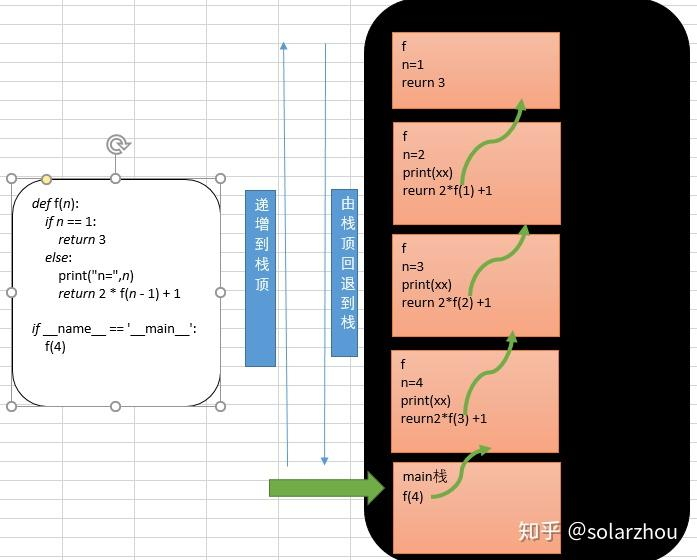
\includegraphics[width=0.7\textwidth]{栈递归.jpg}
    \caption{函数递归调用栈} % 图片标题
    \label{fig:栈递归} % 图片标签，用于引用
\end{figure}

在函数调用时，新的函数的栈帧会被压入栈中(称为栈帧)，从而覆盖掉原来的\textbf{栈帧}，当函数返回时，栈帧会被弹出栈。
露出原来的函数栈帧。当函数调用自身时，会形成一个\textbf{递归调用栈}。

需要注意的是，栈内存的大小是有限制的，当函数调用层次过深时，会出现栈溢出。


\section{本章小结}
本章围绕"组织数据 → 组织函数 → 组织内存 → 组织计算"这条主线展开：

\begin{itemize}
\item \textbf{类与面向对象}：类的三大成员（数据成员、成员函数、构造/析构函数）和三种访问限定符是天天要用的基本功，要求熟练；函数重载、运算符重载、继承与多态是阅读和编写类代码的必备能力；模板只需掌握最基本的函数模板和类模板写法，遇到变参模板等进阶内容会查文档即可。
\item \textbf{lambda、引用与移动}：lambda 的捕获列表（值捕获 vs 引用捕获）和 \texttt{std::function} 承接要熟练使用，回调和排序比较器里到处都是它；左值/右值、两种引用与 \texttt{std::move}/\texttt{std::forward} 是本章最容易混淆的部分，记住"能取地址的是左值、有名字的右值引用是左值"这两句就够应付日常，其余在实践中慢慢消化。
\item \textbf{智能指针}：掌握 \texttt{unique\_ptr}（独占）、\texttt{shared\_ptr}（计数共享）、\texttt{weak\_ptr}（观察不占有）的分工，默认优先 \texttt{make\_unique}/\texttt{make\_shared}；循环引用的成因和用 \texttt{weak\_ptr} 破解的方法必须理解。
\item \textbf{STL}：\texttt{vector} 的常用成员函数和扩容机制要熟练；队列、堆栈、映射等容器知道各自解决什么问题、会去 cppreference 查用法即可；迭代器失效是新手重灾区，删除元素时牢记用 \texttt{erase} 的返回值更新迭代器。
\item \textbf{多线程与内存}：会创建线程，使用 \texttt{mutex}/\texttt{lock\_guard}、共享锁、原子变量和条件变量；能用 \texttt{future}/\texttt{promise}/\texttt{async} 传递异步结果；理解生产者—消费者、读者—写者、哲学家进餐和死锁；进程内存分区（代码/常量/静态/堆/栈）和栈帧机制是理解悬垂指针、栈溢出等经典 bug 的地基，务必建立图景。
\end{itemize}

本章验收通过后，恭喜你已经掌握了阅读现代 C++ 工程代码的主要语法设施。下一章我们来看看这些代码是如何被编译器组装成可执行文件的——CMake 见。

\begin{problemset}
\item 说出 \texttt{public}、\texttt{private}、\texttt{protected} 三种访问限定符的区别，并说明基类的 \texttt{private} 成员能否被派生类直接访问。
\item 判断并说明理由：\texttt{int f(int)} 与 \texttt{double f(int)} 能否构成函数重载？
\item 写出 lambda 表达式的简化语法形式，并说明值捕获 \texttt{[a]} 与引用捕获 \texttt{[\&a]} 在"修改原变量"这一点上的区别。
\item 解释左值与右值的区别，写出判断一个表达式是左值还是右值的最常用方法。
\item 说明 \texttt{std::move} 的作用，并回答：对一个对象执行 \texttt{std::move} 之后，该对象本身的数据被搬走了吗？
\item 比较 \texttt{unique\_ptr} 与 \texttt{shared\_ptr} 的所有权语义，并说明为什么前者的拷贝构造被禁用。
\item 解释 \texttt{shared\_ptr} 循环引用的成因，以及如何用 \texttt{weak\_ptr} 解决。
\item （提高）写出遍历 \texttt{std::vector} 时安全删除满足某条件元素的两种写法（提示：一种利用 \texttt{erase} 的返回值，一种是 erase-remove 惯用法）。
\item （提高）解释死锁产生的四个必要条件，并结合"两把锁以相反顺序获取"的例子说明破坏哪一个条件可以修复它。
\item （实践）综合本章内容实现一个小程序：定义 \texttt{Armor} 类（含编号、置信度数据成员），用 \texttt{std::vector} 管理若干对象，使用 lambda 作为比较器按置信度降序排序，最后以多线程方式（两个线程）分别统计其中置信度高于/低于 0.5 的数量并打印，注意线程安全。
\end{problemset}

% ============================================================
\chapter{编译过程与 CMake 基础}

\begin{introduction}
  \item 学习目标：分步生成编译产物；用 CMake 构建、链接并安装多文件工程；查找 OpenCV 依赖并定位常见构建错误。
  \item 建议学时：约 3--5 天（含练习）。
  \item 本卷边界：只考核标准 C++ 工程与 OpenCV 的基础构建；CUDA、ament 构建细节及图像算法见卷二，章末 ROS2 工程片段为选读。
\end{introduction}

% 仅在本章为较长的命令名留出换行余量。
\begingroup
\setlength{\emergencystretch}{3em}
% Chapter3 原文使用 \subsection 作为章内一级，临时提升为 \section
\let\subsection\section
上一章，我们写了不少 C++ 代码。这一章，一起看看这些代码怎样变成能运行的程序。
先手动走一遍编译过程，再交给 CMake 管理。以后终端刷出一屏报错，你就能先判断卡在哪一步，不用一上来就怀疑人生。

下面的命令都在 Ubuntu 22.04 的 Bash 中运行。每个示例都会写清楚：在哪个目录操作、要建哪些文件、跑完应该看到什么。
打开终端，跟着做就行。

% 保留原有章内一级标题，层级仍由 main.tex 的临时映射控制。
\subsection{C++的编译过程}
\label{sec:build-process}

C++ 从源文件到可执行文件，通常经历以下四步：
\begin{enumerate}
    \item \textbf{预处理（Preprocessing）}：展开头文件、宏和条件编译，得到预处理后的源文件。
    \item \textbf{编译（Compilation）}：检查语法与语义，将预处理结果翻译为汇编代码。
    \item \textbf{汇编（Assembly）}：将汇编代码转换为目标文件（Object File）。
    \item \textbf{链接（Linking）}：把目标文件和所需库组合起来，解析符号引用，生成可执行文件等产物。
\end{enumerate}

\begin{figure}[H]
    \centering
    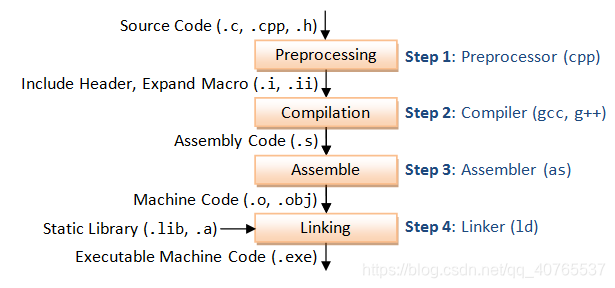
\includegraphics[width=0.7\textwidth]{编译流程.png}
    \caption{C++ 编译过程}
    \label{fig:编译}
\end{figure}

\textbf{预处理：先把这一份源代码准备好}

预处理器先处理那些以 \texttt{\#} 开头的指令。
\texttt{\#include} 引入文件内容，\texttt{\#define} 定义宏，\texttt{\#if} 等指令决定保留哪部分代码。用到宏时，预处理器会按规则展开它。
一个 \texttt{.cpp} 文件，加上它包含的头文件，经过预处理后叫作一个\textbf{翻译单元（Translation Unit）}。
后面编译时，各个翻译单元分别处理。

\begin{note}
同一个头文件，可以在编译不同 \texttt{.cpp} 时分别被处理。
头文件保护（如 \texttt{\#ifndef}/\texttt{\#define}/\texttt{\#endif}）只防止同一翻译单元内重复包含。
写入门工程时，头文件里通常放声明，普通非 \texttt{inline} 函数的定义放在一个 \texttt{.cpp} 里。这样能避免链接时重复定义。
\end{note}

排查问题时，下面这些名字可以帮助定位代码：
\begin{center}
\begin{tabular}{p{0.30\textwidth}p{0.60\textwidth}}
\toprule[1.5pt]
语法 & 作用 \\
\midrule[1pt]
$\_\_FILE\_\_$ & 当前源文件名。\\
$\_\_LINE\_\_$ & 当前源文件行号。\\
$\_\_DATE\_\_$、$\_\_TIME\_\_$ & 源文件被翻译时的日期与时间，不是程序运行时间。\\
$\_\_cplusplus$ & 使用的 C++ 标准版本值；C++17 对应 \texttt{201703L}。\\
$\_\_func\_\_$ & 函数体内可用的标准预定义变量，表示函数名；它不是宏。\\
\bottomrule[1.5pt]
\end{tabular}
\end{center}

\begin{note}
\texttt{\_\_FUNCTION\_\_} 是常见编译器扩展，入门代码优先用 \texttt{\_\_func\_\_}。
\texttt{\_\_STDC\_VERSION\_\_} 表示 C 语言标准版本，不是 C++ 编译器版本；查看 GCC 版本可运行 \texttt{g++ --version}。
\end{note}

\textbf{编译与汇编：检查代码，再生成机器指令}

编译器先分析代码中的词、语法和含义，再生成代码，并按选项进行优化。这些检查分别叫词法、语法和语义分析。
少写分号、调用未声明的函数，通常会在这里报错。

接着，汇编器把汇编代码变成可重定位目标文件（Relocatable Object File）。在 Linux 中，它常以 \texttt{.o} 结尾。
目标文件里有机器代码和数据，还有符号表与重定位信息。你可以先把“符号”理解为函数、变量等的名字。
其中一些符号由本文件定义，另一些还要去其他文件里找。后续链接时，还需要确定相关地址，所以 \texttt{.o} 通常不能直接运行。

\textbf{链接：让调用找到实现}

声明告诉编译器“这个函数怎样调用”，定义给出函数的具体实现。
链接器要把函数调用和对应的实现联系起来，再合并所需代码与数据，处理相关地址。这就是解析符号引用和处理重定位。
如果程序依赖动态库，还会留下一些信息，等加载器处理。

比如，你声明并调用了一个函数，却漏掉了实现所在的目标文件或库。链接器找不到实现，就可能报
\texttt{undefined reference}（未定义引用）。读到这条错误时，先查函数定义有没有参与链接。

\textbf{手动控制四个阶段}

\texttt{g++} 是 GCC 的 C++ 编译驱动程序。通用形式为 $g++\enspace[\text{选项}]\enspace \text{输入文件}\ldots$；不指定停止阶段时，它会继续完成链接。
\begin{center}
\begin{tabular}{p{0.30\textwidth}p{0.60\textwidth}}
\toprule[1.5pt]
参数 & 作用 \\
\midrule[1pt]
$-E$ & 只做预处理。\\
$-S$ & 完成编译后停止，生成汇编文件。\\
$-c$ & 生成目标文件后停止，不链接。\\
$-o\enspace \text{文件}$ & 指定输出文件名。\\
$-std=\text{标准}$ & 选择语言标准，本章使用 \texttt{c++17}。\\
$-I\enspace \text{目录}$ & 增加头文件搜索目录。\\
$-Wall$、$-Wextra$ & 开启常用编译警告。\\
$-g$ & 生成调试信息。\\
\bottomrule[1.5pt]
\end{tabular}
\end{center}
其余参数请查阅 \texttt{man g++} 手册。

\begin{example}[亲眼看到四种产物]
先装好工具，再建一个专门放练习的目录。若你已经用过这个目录名，就换一个，避免覆盖自己的文件。
\begin{tbash}
sudo apt update
sudo apt install build-essential cmake
mkdir -p ~/rm-build-lab/stages
cd ~/rm-build-lab/stages
\end{tbash}
创建 \texttt{hello.cpp}，内容如下：
\begin{tcpp}
#include <iostream>
#define ARMOR_ID 3

int main() {
    std::cout << "armor=" << ARMOR_ID << '\n';
    std::cout << "function=" << __func__ << '\n';
    return 0;
}
\end{tcpp}
留在这个目录里，逐条运行下面的命令。每跑完一步，都看看多了哪个文件：
\begin{tbash}
g++ -std=c++17 -E hello.cpp -o hello.ii
g++ -std=c++17 -S hello.ii -o hello.s
g++ -c hello.s -o hello.o
g++ hello.o -o hello
./hello
\end{tbash}
预期输出两行：\texttt{armor=3} 和 \texttt{function=main}。
再用编辑器打开 \texttt{hello.ii}，搜索 \texttt{armor=}。你会看到这里的 \texttt{ARMOR\_ID} 已经变成了 \texttt{3}。
文件比原来长很多是正常的，头文件内容也被展开进来了。不用从第一页读到最后一页，我们只找刚才那一行。
平时构建时，把这四步交给一条命令就行：
\begin{tbash}
g++ -std=c++17 -Wall -Wextra hello.cpp -o hello
./hello
\end{tbash}
\end{example}

\textbf{静态库与动态库}

有些代码会被多个程序用到，我们可以把它们做成库（Library）。库常见有两种：

\textbf{静态库（Static Library）}通常把多个目标文件打包在一起，Linux 中常见文件名为 \texttt{lib名称.a}。
链接时，链接器把所需目标文件中的代码和数据放进最终产物。

\textbf{动态库或共享库（Shared Library）}在 Linux 中常见文件名为 \texttt{lib名称.so}。
普通动态链接会在构建时记下程序依赖哪些库。程序启动或运行时，再由加载器装入这些库。

\begin{note}
“静态库编译一定更快”和“动态库运行一定更慢”都不是可靠结论。速度取决于具体工程和测量结果。
刚开始先关心一件事：把程序搬到另一台电脑时，还要带上什么？
静态链接某个库后，通常不用再带上这个库的独立文件。动态链接则需要运行环境里有兼容的库。
另外，链接了一个静态库，不代表整个程序都采用了静态链接。性能如何，跑一跑再说，别急着给两种库排战力榜。
\end{note}

\begin{conclusion}
\begin{itemize}
    \item \texttt{.cpp → .ii → .s → .o → 可执行文件} 对应预处理、编译、汇编、链接。
    \item 找不到头文件先查包含路径；语法错误先查源代码；未定义引用先查实现及链接依赖。
    \item 声明用于检查调用，定义提供实现，目标文件承载编译结果，库组织可复用代码。
    \item 静态库与动态库主要影响链接方式和部署条件，不能直接据此判断性能。
\end{itemize}
\end{conclusion}

\begin{exercise}
给装甲板换个编号：把 \texttt{ARMOR\_ID} 改为 \texttt{7}。先直接运行旧的 \texttt{hello}，再重新构建并运行。
两次输出有什么不同？请结合刚才的四步解释原因。
接着故意漏写一个分号，看看哪一步先报错。观察完记得补回来，别给下一节留下伏笔。
\end{exercise}

\subsection{CMake}
\label{sec:cmake-basics}

只有一个源文件时，手写 \texttt{g++} 命令很方便。文件一多，你就得记住：谁依赖谁？哪些文件改过？哪些程序要重新构建？
这些工作可以交给 Make，它按 \texttt{Makefile} 里的规则来做。

\textbf{CMake} 是跨平台的构建系统生成工具。你把工程怎么构建写进 \texttt{CMakeLists.txt}，CMake 再生成 Make、Ninja 或 IDE 使用的构建文件。
之后，相应的构建工具会调用编译器和链接器。
生成器（Generator）决定生成哪种构建文件。CMake 本身不翻译 C++ 代码。

接下来，我们按顺序完成项目配置、添加文件、编译、链接和安装，最后一起读一段实际工程的配置。
先分清三个动作：\textbf{配置与生成}负责读取构建描述、查找依赖、写出构建文件；\textbf{构建}负责真正编译和链接；\textbf{安装}负责按规则复制产物。

看到 \texttt{Configuring done} 和 \texttt{Generating done}，先别开香槟。构建文件准备好了，程序还得接着编译。

\begin{conclusion}
\begin{itemize}
    \item \texttt{CMakeLists.txt} 描述目标和依赖；CMake 读取它并生成构建文件。
    \item Make 或 Ninja 读取生成的规则，安排需要执行的任务。
    \item 编译器和链接器执行这些任务，生成目标文件、库与可执行文件。
    \item 安装按规则复制已有产物；配置成功、构建成功和安装成功是三个不同的检查点。
\end{itemize}
\end{conclusion}

\subsubsection{项目配置}
\label{sec:cmake-config}

先在项目根目录建一个 \texttt{CMakeLists.txt}，文件名的大小写要写对。
里面的命令一般写成 \texttt{命令名(参数...)}。命令名不区分大小写，变量名区分大小写；名称、路径等参数值通常也区分大小写。
开头先写最低 CMake 版本，再用 \texttt{project} 指定语言，让 CMake 检测编译器。

\begin{center}
\begin{tabular}{p{0.49\textwidth}p{0.41\textwidth}}
\toprule[1.5pt]
语法 & 作用 \\
\midrule[1pt]
\texttt{cmake\_minimum\_required(VERSION 版本)} & 声明所需最低版本。\\
\texttt{project(名称 LANGUAGES 语言)} & 设置项目名，启用指定语言。\\
\texttt{set(变量 值...)} & 设置普通变量。\\
\texttt{message(STATUS 内容...)} & 在配置阶段输出信息。\\
\texttt{add\_executable(目标 源文件...)} & 声明一个可执行目标。\\
\texttt{target\_compile\_features(目标 PRIVATE 特性...)} & 为目标指定编译特性，如 C++17。\\
\bottomrule[1.5pt]
\end{tabular}
\end{center}
\texttt{\$\{变量名\}} 表示取变量值，不是 C/C++ 的宏替换。
\texttt{PROJECT\_NAME} 是项目名称，\texttt{CMAKE\_CXX\_COMPILER} 是检测到的 C++ 编译器路径。
\texttt{PRIVATE} 表示这项要求用于当前目标，其他作用域见第~\ref{sec:cmake-scope}~节。

终端命令的通用形式为 $cmake\enspace[\text{选项}]$。构建目录（Build Tree）保存缓存、目标文件和可执行文件，源码目录（Source Tree）保存源代码和构建描述。
\begin{center}
\begin{tabular}{p{0.43\textwidth}p{0.47\textwidth}}
\toprule[1.5pt]
参数 & 作用 \\
\midrule[1pt]
$-S\enspace \text{目录}$ & 指定源码目录。\\
$-B\enspace \text{目录}$ & 指定构建目录，不存在时自动创建。\\
$-D\text{变量}=\text{值}$ & 设置缓存变量，如构建类型。\\
$-G\enspace \text{生成器}$ & 指定生成器，例如 \texttt{Unix Makefiles}。\\
$--build\enspace \text{目录}$ & 调用该构建目录对应的构建工具。\\
$--parallel\enspace \text{数量}$ & 限制并行构建任务数，配合 \texttt{--build} 使用。\\
$--verbose$ & 显示实际构建命令，配合 \texttt{--build} 使用。\\
$--install\enspace \text{目录}$ & 按安装规则复制已构建产物。\\
$--prefix\enspace \text{路径}$ & 指定安装前缀，配合 \texttt{--install} 使用。\\
\bottomrule[1.5pt]
\end{tabular}
\end{center}
其余参数请查阅 \texttt{man cmake}；单条 CMake 语言命令可用 \texttt{cmake --help-command 命令名} 查询。

\begin{example}[先跑通一个最小工程]
在终端新建工程，并复用上节的源文件：
\begin{tbash}
mkdir -p ~/rm-build-lab/hello-cmake
cd ~/rm-build-lab/hello-cmake
cp ../stages/hello.cpp .
\end{tbash}
创建 \texttt{CMakeLists.txt}，完整内容如下。本章采用 CMake 3.16 及以上版本，不需要追求最新版。
\begin{lstlisting}[language=cmake,frame=single,numbers=left]
cmake_minimum_required(VERSION 3.16)
project(hello_cmake LANGUAGES CXX)

set(ARMOR_NAME "training_armor")
message(STATUS "Armor: ${ARMOR_NAME}")
message(STATUS "Compiler: ${CMAKE_CXX_COMPILER}")

add_executable(hello hello.cpp)
target_compile_features(hello PRIVATE cxx_std_17)
\end{lstlisting}
配置、构建和运行：
\begin{tbash}
cmake -S . -B build -DCMAKE_BUILD_TYPE=Debug
cmake --build build --parallel 2
./build/hello
\end{tbash}
配置时应出现 \texttt{Armor: training\_armor} 和编译器路径；运行结果与上节一致。
项目名是 \texttt{hello\_cmake}，目标名是 \texttt{hello}，两者可以不同。
\end{example}

\begin{note}
\texttt{CMakeCache.txt} 会记住编译器、依赖路径等配置。换编译器或生成器时，开一个新的构建目录，别让旧配置继续加戏。
想手动选择 GCC，就在第一次配置时传入 \texttt{-DCMAKE\_CXX\_COMPILER=g++}，不要在 \texttt{project} 后临时修改编译器。
本章使用 Make 等单配置生成器，\texttt{CMAKE\_BUILD\_TYPE=Debug} 用于调试构建；多配置生成器的配置选择用法另查手册。
CUDA 的语言启用与工具链配置见卷二 CUDA 章。
\end{note}

\begin{exercise}
将目标 \texttt{hello} 改名为 \texttt{armor\_hello}，同步修改对应的目标配置，使用新的 \texttt{build-rename} 目录构建并运行。
说明为什么不需要修改 \texttt{project(hello\_cmake ...)}。
\end{exercise}

\subsubsection{添加文件}
\label{sec:cmake-files}

文件准备好后，还得告诉 CMake 怎样使用它们。这里有三件事：列出要编译的源文件、设置头文件搜索目录、查找外部依赖。
CMake 把一个可执行程序或一个库称为目标（Target），后面的配置大多围绕目标来写。
这三件事要分别完成：设置头文件搜索目录不会自动添加源文件，\texttt{find\_package} 也不会替你下载和安装依赖。

\begin{center}
\begin{tabular}{p{0.46\textwidth}p{0.44\textwidth}}
\toprule[1.5pt]
语法 & 作用 \\
\midrule[1pt]
\texttt{set(变量 源文件...)} & 保存显式源文件列表。\\
\texttt{target\_include\_directories(目标 作用域 目录...)} & 为目标设置头文件搜索目录。\\
\texttt{find\_package(包名 REQUIRED)} & 查找已安装的包，缺失时终止配置。\\
\texttt{option(变量 "说明" 默认值)} & 声明可由命令行设置的布尔开关。\\
\texttt{if(条件) ... endif()} & 根据条件执行 CMake 命令。\\
\texttt{target\_compile\_definitions(目标 作用域 宏...)} & 向目标的编译过程传入宏定义。\\
\bottomrule[1.5pt]
\end{tabular}
\end{center}

\begin{example}[为装甲板程序准备三个文件]
\label{ex:armor-sources}
来写一个给装甲板打分的小程序。从这里到安装一节，我们一直用这个 \texttt{armor-demo} 工程，不用每节重新建一套文件。先建目录：
\begin{tbash}
mkdir -p ~/rm-build-lab/armor-demo/include
mkdir -p ~/rm-build-lab/armor-demo/src
cd ~/rm-build-lab/armor-demo
\end{tbash}
创建 \texttt{include/armor.hpp}，只声明接口，并加上头文件保护：
\begin{tcpp}
#ifndef ARMOR_DEMO_ARMOR_HPP
#define ARMOR_DEMO_ARMOR_HPP

int armor_score(int id);

#endif
\end{tcpp}
创建 \texttt{src/armor.cpp}，提供函数定义：
\begin{tcpp}
#include "armor.hpp"

int armor_score(int id) {
    return id * 10;
}
\end{tcpp}
创建 \texttt{src/main.cpp}，使用接口：
\begin{tcpp}
#include "armor.hpp"
#include <iostream>

int main() {
    std::cout << "score=" << armor_score(3) << '\n';
#ifdef SAVE_OUTPUT
    std::cout << "save output enabled\n";
#endif
    return 0;
}
\end{tcpp}
暂时先用上节学过的编译命令验证文件齐全：
\begin{tbash}
g++ -std=c++17 -I include src/main.cpp src/armor.cpp -o armor_manual
./armor_manual
\end{tbash}
预期输出 \texttt{score=30}。其中 \texttt{-I include} 让两个源文件都能找到 \texttt{armor.hpp}。
接下来会为它创建完整的 CMake 构建描述。
\end{example}

头文件通常不用单独编译，但编译器必须找得到它。
你列出要编译的源文件，CMake 据此安排构建。编译器再按包含规则查找头文件，并记录文件之间的依赖，供后续增量构建使用。
所以，源文件列表和头文件路径都要写清楚。

\begin{note}
旧工程可能用 \texttt{file(GLOB\_RECURSE 变量 路径模式)} 递归收集源文件。
我们先把源文件一个个列出来。以后加文件，就顺手改一次列表，检查起来也方便。
用通配符时，要小心把其他程序的 \texttt{main.cpp} 也收进来。两个入口争当主角，链接器可不会帮你选。
\texttt{include\_directories} 设置头文件搜索路径，\texttt{link\_directories} 设置库搜索路径；二者都不等于“把实现链接进程序”。
\end{note}

\begin{exercise}
做两次小型排错练习，每次都从完整命令开始：第一次去掉 \texttt{-I include}，第二次去掉 \texttt{src/armor.cpp}。
分别读一读报错，判断哪次找不到头文件、哪次找不到函数实现。最后恢复完整命令，确认程序能运行。
\end{exercise}

\subsubsection{编译}
\label{sec:cmake-build}

用下面两种形式分别声明可执行目标和库目标：
\begin{quote}
$add\_executable(\text{目标}\enspace \text{源文件}\ldots)$\\
$add\_library(\text{目标}\enspace[\text{类型}]\enspace \text{源文件}\ldots)$
\end{quote}
这两条命令先记下“要构建什么”。等你运行构建命令时，编译器才开始工作。

\begin{center}
\begin{tabular}{p{0.30\textwidth}p{0.60\textwidth}}
\toprule[1.5pt]
参数 & 作用 \\
\midrule[1pt]
目标 & 工程中唯一的逻辑名称，供后续 \texttt{target\_*} 命令引用。\\
源文件 & 要编译的 \texttt{.cpp} 文件，可显式列出或通过变量展开。\\
$STATIC$ & 生成静态库。\\
$SHARED$ & 生成共享库。\\
省略类型 & 根据 \texttt{BUILD\_SHARED\_LIBS} 选择；未设置或为假时默认静态库。\\
\bottomrule[1.5pt]
\end{tabular}
\end{center}

下面还会用到 \texttt{target\_compile\_options}，它为指定目标添加编译选项。
通用形式为：
\begin{quote}
$target\_compile\_options(\text{目标}\enspace \text{作用域}\enspace \text{选项}\ldots)$
\end{quote}
本节用 \texttt{PRIVATE} 把 \texttt{-Wall} 和 \texttt{-Wextra} 仅加给当前目标。
这些选项适用于 GCC、Clang，因此示例先检查编译器标识，再添加它们。
其他选项可查阅编译器手册；这条 CMake 命令的参数可用
\texttt{cmake --help-command target\_compile\_options} 查询。

\begin{example}[一次构建两个源文件]
在示例~\ref{ex:armor-sources}~的 \texttt{armor-demo} 根目录创建 \texttt{CMakeLists.txt}：
\begin{lstlisting}[language=cmake,frame=single,numbers=left]
cmake_minimum_required(VERSION 3.16)
project(armor_demo LANGUAGES CXX)

set(ARMOR_SOURCES src/main.cpp src/armor.cpp)
add_executable(armor_demo ${ARMOR_SOURCES})
target_include_directories(armor_demo PRIVATE
    "${CMAKE_CURRENT_SOURCE_DIR}/include")
target_compile_features(armor_demo PRIVATE cxx_std_17)

if(CMAKE_CXX_COMPILER_ID MATCHES "GNU|Clang")
    target_compile_options(armor_demo PRIVATE -Wall -Wextra)
endif()

option(SAVE_OUTPUT "Enable save-output message" OFF)
if(SAVE_OUTPUT)
    target_compile_definitions(armor_demo PRIVATE SAVE_OUTPUT)
endif()
\end{lstlisting}
\texttt{CMAKE\_CURRENT\_SOURCE\_DIR} 是当前处理的源码目录。
警告选项只加给当前目标；开关只演示条件编译，\textbf{并不真的保存文件}。
\begin{tbash}
cmake -S . -B build -DCMAKE_BUILD_TYPE=Debug
cmake --build build --parallel 2
./build/armor_demo
cmake -S . -B build -DSAVE_OUTPUT=ON
cmake --build build --parallel 2
./build/armor_demo
\end{tbash}
第一次输出 \texttt{score=30}；打开开关并重新构建后，多一行 \texttt{save output enabled}。
\end{example}

\begin{note}
CMake 变量和 C++ 宏处在不同阶段。\texttt{option(SAVE\_OUTPUT ...)} 创建的是配置开关；
\texttt{target\_compile\_definitions} 才把它转换成该目标编译时可见的宏。
\texttt{add\_library(name ...)} 也不保证生成动态库，需要动态库时明确写 \texttt{SHARED}。
\end{note}

\begin{exercise}
给 3 号装甲板开一次“双倍积分”：把 \texttt{armor\_score} 中的乘数改成 \texttt{20}。
只执行构建和运行命令，检查输出是否变成 \texttt{score=60}。
再用 \texttt{-DSAVE\_OUTPUT=OFF} 重新配置并构建，确认提示消失。练完把乘数改回 \texttt{10}，活动结束，积分恢复正常。
\end{exercise}

\subsubsection{链接}
\label{sec:cmake-link}

如果几个程序都要用装甲板打分函数，我们可以把实现做成一个库，让这些程序链接它。
通用形式为：
\begin{quote}
$target\_link\_libraries(\text{目标}\enspace \text{作用域}\enspace \text{依赖}\ldots)$
\end{quote}
第一个参数是已经创建的\textbf{目标名}，不是 \texttt{.o} 文件名。

\begin{center}
\begin{tabular}{p{0.30\textwidth}p{0.60\textwidth}}
\toprule[1.5pt]
参数 & 作用 \\
\midrule[1pt]
目标 & 需要链接依赖的可执行目标或库目标。\\
$PRIVATE$ & 当前目标使用这项依赖；其接口不要求使用者直接使用它。\\
$PUBLIC$ & 当前目标使用依赖，其使用接口也向下游传播。\\
$INTERFACE$ & 仅作为接口要求提供给下游，当前目标不用于自身链接。\\
依赖 & 可为本工程的库目标、包提供的导入目标或库路径等。\\
\bottomrule[1.5pt]
\end{tabular}
\end{center}
链接本工程的库目标时，直接写目标名，CMake 会安排好构建顺序，并找到对应的库文件。
注意 \texttt{armor} 和 \texttt{\$\{armor\}} 的区别：前者是目标名，后者在读取同名变量。如果没设置这个变量，读到的值就可能是空的。

\begin{example}[把实现拆成静态库]
\label{ex:armor-library}
保持三个 C++ 文件不变，将 \texttt{armor-demo/CMakeLists.txt} \textbf{完整替换}为下面内容：
\begin{lstlisting}[language=cmake,frame=single,numbers=left]
cmake_minimum_required(VERSION 3.16)
project(armor_demo LANGUAGES CXX)

add_library(armor STATIC src/armor.cpp)
target_include_directories(armor PUBLIC
    "${CMAKE_CURRENT_SOURCE_DIR}/include")
target_compile_features(armor PUBLIC cxx_std_17)

add_executable(armor_demo src/main.cpp)
target_link_libraries(armor_demo PRIVATE armor)

if(CMAKE_CXX_COMPILER_ID MATCHES "GNU|Clang")
    target_compile_options(armor PRIVATE -Wall -Wextra)
    target_compile_options(armor_demo PRIVATE -Wall -Wextra)
endif()

option(SAVE_OUTPUT "Enable save-output message" OFF)
if(SAVE_OUTPUT)
    target_compile_definitions(armor_demo PRIVATE SAVE_OUTPUT)
endif()
\end{lstlisting}
使用新的构建目录，方便与上一版对照：
\begin{tbash}
cmake -S . -B build-lib -DCMAKE_BUILD_TYPE=Debug
cmake --build build-lib --parallel 2
./build-lib/armor_demo
ls build-lib/libarmor.a
\end{tbash}
预期运行输出 \texttt{score=30}，并能看到静态库 \texttt{libarmor.a}。
\texttt{armor} 把头文件目录设为 \texttt{PUBLIC}，所以链接它的 \texttt{armor\_demo} 也能找到接口头文件。
\end{example}

\begin{conclusion}
\begin{itemize}
    \item \texttt{add\_executable}/\texttt{add\_library} 创建目标；\texttt{target\_*} 为已存在的目标补充要求。
    \item 包含目录解决“头文件在哪”；链接依赖解决“函数实现在哪”；两者各有用途。
    \item 链接一个库目标会带来它公开的使用要求，例如头文件搜索目录。
    \item 静态库的 \texttt{PRIVATE} 依赖仍可能成为最终可执行程序必需的链接项，不能理解成“下游链接命令绝不会出现它”。
\end{itemize}
遇到未定义引用，就沿着这几步查。链接器不接受“我记得写过这个函数”作为证据，得让它真的找到实现。
\end{conclusion}

\begin{exercise}
在 Ubuntu 中把库类型改为 \texttt{SHARED}，用新目录 \texttt{build-shared} 配置、构建并运行，观察生成的 \texttt{libarmor.so}。
记录动态库的文件名，随后将源码中的类型恢复为 \texttt{STATIC}，后续安装示例使用静态库版本。
\end{exercise}

\subsubsection{安装}
\label{sec:cmake-install}

程序已经能在构建目录里运行了。接下来，我们把它放到指定位置，方便以后使用，这一步叫安装（Install）。
按目标声明安装规则的通用形式为：
\begin{quote}
$install(TARGETS\enspace \text{目标}\ldots\enspace[\text{产物类别}\enspace DESTINATION\enspace \text{目录}]\ldots)$
\end{quote}
\begin{center}
\begin{tabular}{p{0.30\textwidth}p{0.60\textwidth}}
\toprule[1.5pt]
参数 & 作用 \\
\midrule[1pt]
$TARGETS$ & 后接已创建的目标名，不写源文件名。\\
$RUNTIME$ & 选择运行时产物；本章用它安装可执行文件。\\
$ARCHIVE$ & 选择归档产物；在本章的 Linux 环境中可用于静态库。\\
$LIBRARY$ & 选择库产物；在本章的 Linux 环境中可用于共享库。\\
$DESTINATION\enspace \text{目录}$ & 指定安装目录；相对目录按安装前缀解析。\\
\bottomrule[1.5pt]
\end{tabular}
\end{center}
本节只安装可执行文件，使用 \texttt{RUNTIME DESTINATION bin}。
安装前缀由终端中的 \texttt{--prefix} 指定；\texttt{bin} 是前缀下的子目录。
其余参数请查阅 \texttt{cmake --help-command install}。

\begin{example}[安装到自己的练习目录]
在示例~\ref{ex:armor-library}~的 \texttt{CMakeLists.txt} 末尾追加：
\begin{lstlisting}[language=cmake,frame=single,numbers=left]
install(TARGETS armor_demo RUNTIME DESTINATION bin)
\end{lstlisting}
在 \texttt{armor-demo} 根目录运行：
\begin{tbash}
cmake -S . -B build-lib -DCMAKE_BUILD_TYPE=Debug
cmake --build build-lib --parallel 2
cmake --install build-lib --prefix "$PWD/stage"
./stage/bin/armor_demo
\end{tbash}
预期出现安装路径 \texttt{stage/bin/armor\_demo}，运行输出 \texttt{score=30}。
该程序已静态链接我们编写的 \texttt{armor} 库，因此这里无需安装独立的 \texttt{libarmor.a}。
\end{example}

\begin{note}
\texttt{cmake --install} 不会自动构建，记得按“配置 → 构建 → 安装”的顺序来。
安装可能覆盖目标位置的同名文件。练习时就用自己的 \texttt{stage} 目录，不需要 \texttt{sudo}，先别急着往系统目录里搬。
如果换成动态库版本，还要带上所需共享库，并设置好运行时搜索路径。只复制一个可执行文件，到了另一台电脑上可能跑不起来。相关细节以后做部署时再展开。
\end{note}

\begin{exercise}
不修改安装规则，将同一程序安装到 \texttt{stage-check} 目录，并从那里运行。
指出安装前缀和 \texttt{DESTINATION bin} 分别对应最终路径的哪一部分。
\end{exercise}

\subsubsection{补充内容}
\label{sec:cmake-scope}

\textbf{目录设置与目标设置}

读旧工程时，你可能会遇到 \texttt{include\_directories}。它会影响当前目录及相关子目录、目标的包含目录设置，不能简单理解成“整个工程都生效”。
我们先用 \texttt{target\_include\_directories} 这类命令：哪个目标需要，就给哪个目标设置。
这里的 \texttt{PRIVATE}、\texttt{PUBLIC}、\texttt{INTERFACE} 决定谁会用到这些配置。名字可能眼熟，但它们和 C++ 类的访问权限是两回事。

\begin{conclusion}
以头文件路径和编译特性为例，三种作用域可这样判断：
\begin{itemize}
    \item \texttt{PRIVATE}：当前目标自己用，例如库内部实现专用的包含目录。
    \item \texttt{PUBLIC}：当前目标和使用它的下游都用，例如示例中的 \texttt{armor.hpp} 所在目录。
    \item \texttt{INTERFACE}：仅下游使用，常见于只提供头文件的接口库。
\end{itemize}
\end{conclusion}

\textbf{把调试函数放进单独的文件}

配置出了问题，又看不出变量里装着什么，就先把它打印出来。
我们把打印操作写成函数，再放进单独的文件，以后就能重复使用。
自定义函数写成 \texttt{function(函数名 参数...) ... endfunction()}。
\texttt{include(模块名)} 用来载入模块，\texttt{list(APPEND 变量 元素...)} 用来往列表中追加元素。
\texttt{CMAKE\_MODULE\_PATH} 是查找自定义模块时使用的目录列表。
把 \texttt{cmake} 目录加入它后，\texttt{include(Function)} 就能找到其中的 \texttt{Function.cmake}。
函数中的 \texttt{if(DEFINED 变量名)} 检查变量是否已定义；已定义但值为空，和根本没定义是两种情况。

\begin{example}[打印编译器与构建类型]
先在 \texttt{armor-demo} 根目录创建模块目录：
\begin{tbash}
mkdir -p cmake
\end{tbash}
新建 \texttt{cmake/Function.cmake}，写入：
\begin{lstlisting}[language=cmake,frame=single,numbers=left]
function(print_var var)
    if(DEFINED ${var})
        message(STATUS "${var} = [${${var}}]")
    else()
        message(STATUS "${var} is not defined")
    endif()
endfunction()
\end{lstlisting}
在 \texttt{CMakeLists.txt} 的 \texttt{project} 后加入：
\begin{lstlisting}[language=cmake,frame=single,numbers=left]
list(APPEND CMAKE_MODULE_PATH
    "${CMAKE_CURRENT_SOURCE_DIR}/cmake")
include(Function)
print_var(CMAKE_CXX_COMPILER)
print_var(CMAKE_BUILD_TYPE)
print_var(NOT_DEFINED_YET)
\end{lstlisting}
运行 \texttt{cmake -S . -B build-lib -DCMAKE\_BUILD\_TYPE=Debug}，预期打印编译器路径、\texttt{Debug} 和未定义变量提示。
\texttt{var} 接收的是变量名。读 \texttt{\$\{\$\{var\}\}} 时，从里往外看：先拿到名字，再读取这个名字对应的值。
空字符串也可以直接输出，不用特意截取最后一个字符或补换行。
\end{example}

\begin{figure}[H]
    \centering
    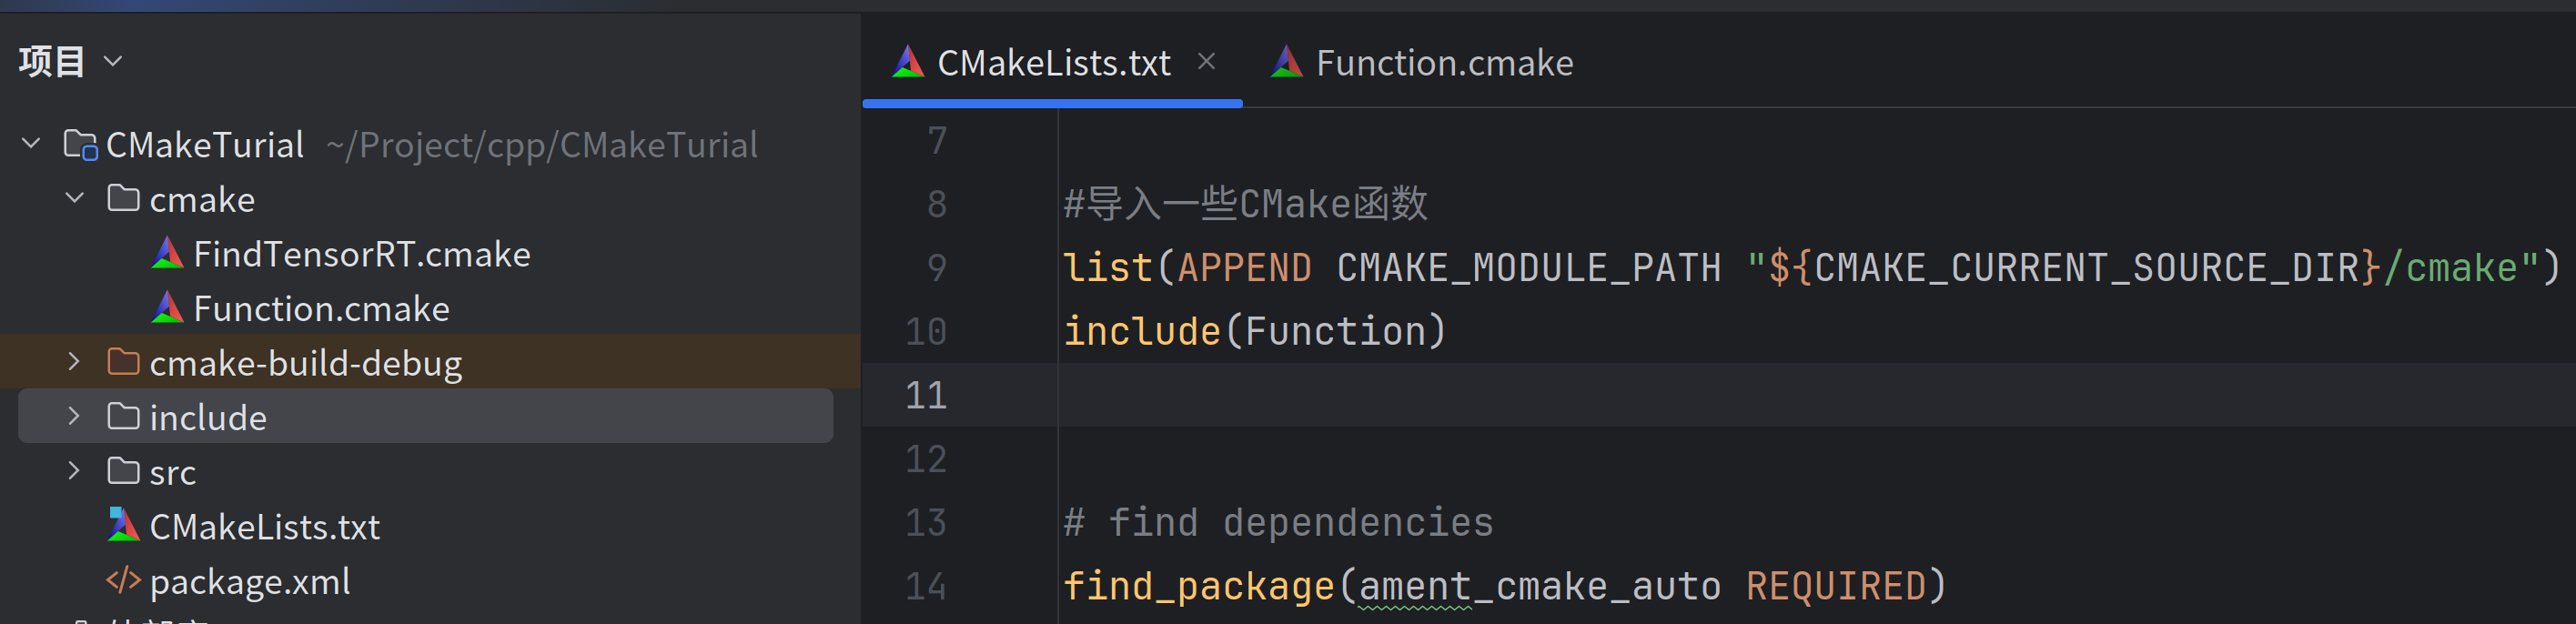
\includegraphics[width=0.7\textwidth]{cmake函数.png}
    \caption{原工程中拆分 CMake 函数文件的结构示意；练习以正文给出的文件路径为准}
    \label{fig:cmakeFunction}
\end{figure}

\textbf{按失败阶段排查}

先别和满屏红字对线，我们从第一处错误看起。
后面的“构建失败”往往只是前面出错后的结果。先判断它发生在哪个阶段，再按下面的方向查，通常比盲目改配置省事。
\begin{center}
\begin{tabular}{p{0.39\textwidth}p{0.51\textwidth}}
\toprule[1.5pt]
命令 / 现象 & 作用 / 排查方向 \\
\midrule[1pt]
配置时报找不到包 & 检查开发包是否安装，以及包配置文件路径。\\
\texttt{No such file or directory}（头文件） & 检查文件名与目标的包含目录。\\
\texttt{undefined reference} & 检查函数定义、签名，以及源文件或库是否参与链接。\\
\texttt{multiple definition} & 检查普通函数是否被重复定义或重复加入目标。\\
\texttt{error while loading shared libraries} & 程序已构建，但运行时找不到所需共享库。\\
\texttt{cmake --build build-lib --verbose} & 查看实际编译与链接命令；无改动时可能没有命令可显示。\\
\bottomrule[1.5pt]
\end{tabular}
\end{center}

\begin{exercise}
在静态库示例中把 \texttt{armor} 的包含目录作用域从 \texttt{PUBLIC} 改为 \texttt{PRIVATE}，重新构建。
指出失败的是库还是可执行目标，解释原因并恢复原配置。
\end{exercise}

\subsubsection{实例}
\label{sec:cmake-opencv}

\textbf{使用外部依赖：OpenCV 图像读取}

自己的库已经能用了，再试试别人写好的 OpenCV。
步骤还是刚才那几步：查找依赖、创建目标、设置包含目录、链接依赖。
\texttt{find\_package(OpenCV REQUIRED)} 查找 OpenCV 提供的包信息；
\texttt{OpenCV\_INCLUDE\_DIRS} 是包含目录，\texttt{OpenCV\_LIBS} 是需要链接的库列表。

\begin{example}[从零编译并显示图像]
在 Ubuntu 桌面环境中安装开发包，建立独立目录：
\begin{tbash}
sudo apt install libopencv-dev
mkdir -p ~/rm-build-lab/opencv-demo
cd ~/rm-build-lab/opencv-demo
\end{tbash}
创建 \texttt{main.cpp}：
\begin{tcpp}
#include <opencv2/opencv.hpp>
#include <iostream>

int main(int argc, char** argv) {
    if (argc != 2) {
        std::cerr << "Usage: image_viewer <image_path>\n";
        return 1;
    }
    const cv::Mat image = cv::imread(argv[1]);
    if (image.empty()) {
        std::cerr << "Cannot read image: " << argv[1] << '\n';
        return 2;
    }
    std::cout << "size=" << image.cols << 'x' << image.rows << '\n';
    cv::imshow("Armor image", image);
    cv::waitKey(0);
    return 0;
}
\end{tcpp}
创建 \texttt{CMakeLists.txt}：
\begin{lstlisting}[language=cmake,frame=single,numbers=left]
cmake_minimum_required(VERSION 3.16)
project(opencv_demo LANGUAGES CXX)

find_package(OpenCV REQUIRED)
add_executable(image_viewer main.cpp)
target_compile_features(image_viewer PRIVATE cxx_std_17)
target_include_directories(image_viewer PRIVATE ${OpenCV_INCLUDE_DIRS})
target_link_libraries(image_viewer PRIVATE ${OpenCV_LIBS})
\end{lstlisting}
先生成一张纯文本格式的测试图，不需要额外下载素材：
\begin{tbash}
printf 'P3\n2 2\n255\n255 0 0  0 255 0\n0 0 255  255 255 255\n' > test.ppm
cmake -S . -B build -DCMAKE_BUILD_TYPE=Debug
cmake --build build --parallel 2
./build/image_viewer test.ppm
\end{tbash}
运行后应输出 \texttt{size=2x2}，并打开显示测试图的窗口。在图像窗口中按任意键，程序就会结束。
这张图只有四个像素，先委屈一下你的显卡。跑通后，再换成自己拍的装甲板图像。

顺便检查两种出错情况：传入不存在的图片路径，程序应提示读取失败，返回 \texttt{2}；不传参数，程序应打印用法，返回 \texttt{1}。
\end{example}

\begin{note}
显示图像需要图形桌面。如果你在纯命令行服务器上操作，或远程连接没有配置图形转发，窗口可能打不开。先检查运行环境，别急着重写构建文件。
如果配置时就找不到 OpenCV，先确认装了开发包 \texttt{libopencv-dev}。Python 的 \texttt{opencv-python} 不能替代它。
如果 OpenCV 是你自己安装的，就找到 \texttt{OpenCVConfig.cmake}，再用 \texttt{-DOpenCV\_DIR=目录} 指向它所在的目录。这里不能随手填一个头文件目录。
\end{note}

\textbf{阅读原有 ROS2 工程片段（选读）}

最后看一眼实际工程，就当是卷二的预告片。
下面这段来自一个包含 Kalman、MLS、LMS 模块的 ROS2 工程。先找一找模块目录、库目标和链接关系，看看能认出多少熟面孔。

这是\textbf{工程阅读片段}。要运行它，还需要原工程的源文件、\texttt{package.xml}、自定义函数文件和 ROS2 环境，不能单独复制出来构建。
ament 的完整用法放在卷二 ROS2 章，这里先读懂主线就够了。

\begin{lstlisting}[language=cmake,frame=single,numbers=left]
cmake_minimum_required(VERSION 3.16)
project(filter LANGUAGES CXX)

list(APPEND CMAKE_MODULE_PATH "${CMAKE_CURRENT_SOURCE_DIR}/cmake")
include(Function)
find_package(ament_cmake_auto REQUIRED)
ament_auto_find_build_dependencies()
find_package(OpenCV REQUIRED)
find_package(Eigen3 REQUIRED)

set(KALMAN_INCLUDE_DIR "${PROJECT_SOURCE_DIR}/include/kalman")
set(MLS_INCLUDE_DIR "${PROJECT_SOURCE_DIR}/include/mls")
set(LMS_INCLUDE_DIR "${PROJECT_SOURCE_DIR}/include/lms")
set(EXEC_INCLUDE_DIR "${PROJECT_SOURCE_DIR}/include/exec")

# 保留旧工程的源文件收集方式，新工程优先显式列出文件。
file(GLOB_RECURSE KALMAN_SRCS "${PROJECT_SOURCE_DIR}/src/kalman/*.cpp")
file(GLOB_RECURSE MLS_SRCS "${PROJECT_SOURCE_DIR}/src/mls/*.cpp")
file(GLOB_RECURSE LMS_SRCS "${PROJECT_SOURCE_DIR}/src/lms/*.cpp")
file(GLOB_RECURSE EXEC_SRCS "${PROJECT_SOURCE_DIR}/src/exec/*.cpp")

set(ALL_INCLUDE ${KALMAN_INCLUDE_DIR} ${MLS_INCLUDE_DIR}
    ${LMS_INCLUDE_DIR} ${EXEC_INCLUDE_DIR} ${OpenCV_INCLUDE_DIRS})
include_directories(${ALL_INCLUDE})
print_var(ALL_INCLUDE)

add_library(filter_kalman STATIC ${KALMAN_SRCS})
add_library(filter_mls STATIC ${MLS_SRCS})
add_library(filter_lms STATIC ${LMS_SRCS})
set(FILTER_LIBS filter_kalman filter_mls filter_lms)
foreach(lib IN LISTS FILTER_LIBS)
    target_compile_features(${lib} PUBLIC cxx_std_17)
    target_link_libraries(${lib} PUBLIC Eigen3::Eigen ${OpenCV_LIBS})
endforeach()

ament_auto_add_executable(filter ${EXEC_SRCS})
# 保留 ament 宏使用的无作用域签名，避免对同一目标混用签名。
target_link_libraries(filter ${FILTER_LIBS})

if(BUILD_TESTING)
    find_package(ament_lint_auto REQUIRED)
    ament_lint_auto_find_test_dependencies()
endif()
ament_auto_package()
\end{lstlisting}

\begin{note}
自动依赖查找命令依据 ROS2 包清单工作。
\texttt{ament\_auto\_add\_executable} 处理可执行目标的相关约定，
\texttt{ament\_auto\_package} 处理包的安装与导出约定。它们不是普通 CMake 命令的通用替代品。
上面的目录设置沿用了原工程的写法。每个库到底需要哪些依赖，还得看对应源码。
这些命令先混个脸熟，不用今天就把卷二速通；本章验收不考它们。
\end{note}

\begin{conclusion}
读陌生构建文件时，先回答三个问题：
\begin{itemize}
    \item 依赖什么：找 \texttt{find\_package}。
    \item 生成什么：找 \texttt{add\_executable} 和 \texttt{add\_library}。
    \item 谁链接谁：找 \texttt{target\_link\_libraries}。
\end{itemize}
找到这三处，再回头看变量和条件分支。第一次读不完很正常，先把程序怎么构建说明白，就已经有收获了。
\end{conclusion}

\begin{note}
参数查阅入口：
\begin{itemize}
    \item GCC 编译阶段与选项：\\
    \url{https://gcc.gnu.org/onlinedocs/gcc/Overall-Options.html}
    \item CMake 构建模型：\\
    \url{https://cmake.org/cmake/help/latest/manual/cmake-buildsystem.7.html}
    \item OpenCV 的 CMake 示例：\\
    \url{https://docs.opencv.org/4.x/db/df5/tutorial_linux_gcc_cmake.html}
\end{itemize}
查到当前问题需要的那一条就好，不用把手册从头刷到尾。其他功能，等用到时再回来查。
\end{note}

\begin{exercise}
回到本节的 \texttt{opencv-demo} 工程，不传参数运行程序，再传入不存在的 \texttt{missing.png}。
每次运行后立刻执行 \texttt{echo \$?}，检查退出码分别为 \texttt{1} 和 \texttt{2}。
说明为什么这两种错误不需要修改链接配置。本题不要求运行上面的 ROS2 选读片段。
\end{exercise}

\makeatletter
\let\subsection\textbook@subsection
\makeatother

\clearpage
\section{本章小结}
这一章，我们把代码一步步变成了能运行的程序。回头看，最常用的是这几件事：
\begin{itemize}
    \item \textbf{看懂编译过程}：说清预处理、编译、汇编和链接各做什么，能区分声明与定义、头文件与目标文件、静态库与动态库。四步命令亲手跑过即可，日常交给构建工具。
    \item \textbf{跑通 CMake 工作流}：用 \texttt{cmake -S/-B} 配置，用 \texttt{cmake --build} 构建，再用 \texttt{cmake --install} 安装。这几条要练熟，源码目录和构建目录也要分开。
    \item \textbf{写清目标与依赖}：先用 \texttt{add\_executable} 或 \texttt{add\_library} 创建目标，再给它设置头文件路径和链接依赖。这部分要会写，也要能说出哪些配置只给自己用，哪些会传给下游。
    \item \textbf{按阶段排错}：先判断卡在配置、编译、链接还是运行，再查相应的路径、实现或依赖。参数细节、自定义模块和 ROS2 的构建约定，用到时会查就行。
\end{itemize}
现在拿一份构建文件，试着说出它要生成什么、依赖什么、怎样运行验证。能说清，也能亲手跑通，就可以带着这些基本功去卷二了。
以后再遇到满屏报错，至少知道从哪里查起——这已经比对着终端许愿靠谱多了。

\begin{problemset}
\item （基础）写出从 \texttt{demo.cpp} 到可执行文件的四个阶段及其中间文件扩展名，并说明 \texttt{g++ -c demo.cpp} 停在哪一步。
\item （基础）你把项目命名为 \texttt{training}，把可执行目标命名为 \texttt{viewer}。这两个名字分别管什么？终端出现 \texttt{Generating done} 时，程序已经编译好了吗？
\item （基础）程序需要 \texttt{main.cpp} 和 \texttt{score.cpp}，头文件放在 \texttt{include} 目录。你已经设置了头文件搜索路径，还需要把 \texttt{score.cpp} 加进目标吗？说说理由。
\item （基础）比较 \texttt{add\_library(score STATIC score.cpp)}、显式写 \texttt{SHARED} 和省略类型三种写法的含义。
\item （基础）你用 \texttt{add\_library(score STATIC score.cpp)} 创建了库，但没定义名为 \texttt{score} 的变量。链接时写 \texttt{score} 和 \texttt{\$\{score\}}，结果一样吗？
\item （基础）安装规则的目标目录为 \texttt{bin}，安装前缀为 \texttt{/home/student/demo-stage}。目标 \texttt{viewer} 会安装到哪里？只运行安装命令能否替代构建？
\item （基础）库需要两个头文件目录：一个是库自己和使用这个库的程序都要用的，另一个只供库内部使用。它们分别该设成什么作用域？\texttt{INTERFACE} 又适合什么情况？
\item （基础）\texttt{find\_package(OpenCV REQUIRED)} 在配置阶段失败。它会自动安装 OpenCV 吗？自行安装 OpenCV 后，\texttt{OpenCV\_DIR} 应指向哪类目录？
\item （提高）你把 \texttt{SAVE\_OUTPUT} 从 \texttt{OFF} 改成 \texttt{ON}，配置完成后就运行了原程序，却没看到新提示。请按 CMake 变量、编译宏、可执行文件的顺序，解释中间漏了哪一步。
\item （实践）观察一次“哪些文件需要重新编译”。在静态库工程中，先不改任何文件，连续构建两次；然后只改 \texttt{src/armor.cpp} 中的乘数，再构建一次。用 \texttt{--verbose} 保存后两次构建的输出，看看各自做了哪些工作。最后把乘数改回来。
\end{problemset}

\endgroup

\chapter*{卷一小结}
\addcontentsline{toc}{chapter}{卷一小结}
\markboth{卷一小结}{卷一小结}
% 卷末回顾：由 main.tex 的无编号章引入，不改变正文层级与习题编号。
\begingroup
% 避免段落或列表项只留一行在相邻页。
\clubpenalty=10000
\widowpenalty=10000
本卷从安装 Ubuntu 开始，经过命令行、版本管理和现代 C++，最后走到了多文件工程的构建与运行。
这些内容共同回答一个问题：\textbf{拿到一份 C++ 工程，怎样在自己的电脑上读懂它、修改它、构建它，并把可验证的修改交给队友？}
卷首介绍的视觉组职责，也因此有了具体的落脚点：图像处理、目标识别与后续决策需要算法，而算法要成为可以协作开发、稳定运行的程序，还需要本卷这些基本功。

下面按三章回顾知识，再把它们放回同一条开发流程中。复习时可以一边读，一边打开终端或已有练习工程验证。
正文中已经给出的安装步骤、代码示例和参数表，仍是动手时的查阅入口；这里着重说明每部分解决什么问题、与其他内容怎样衔接，以及应该掌握到什么程度。

\subsubsection*{一、Linux 工作环境：让开发有一个可靠的起点}

\textbf{1. 安装系统：先认清磁盘，再建立工作环境。}
双系统安装依次涉及分区、制作启动盘、从 U 盘安装和安装后的系统设置。
分区决定两套系统各自使用哪些存储空间，启动盘提供安装环境，安装时的挂载点决定 Linux 如何使用这些分区。
复习时应能说明根目录 \texttt{/}、家目录 \texttt{/home}、交换空间与 EFI 系统分区各自的用途，并能对照自己的磁盘布局指出对应位置。
安装界面上的设备名、容量、文件系统和挂载点，要结合实际机器核对，不能照搬截图中的盘符与数字。

安装完成的判断也要落到操作上：Ubuntu 和 Windows 都能正常启动，网络与常用外设可用，能够打开终端、安装软件并保存自己的文件。
系统扩容、GRUB 引导菜单美化和桌面美化属于选修；前者服务于空间调整，后两者改善使用体验。
遇到这类需要时，应回到对应小节查具体步骤，并先确认当前系统与磁盘的状态。

\textbf{2. 备份与恢复：给环境修改留下退路。}
本章介绍了 Timeshift 系统快照和用 \texttt{tar} 打包的系统备份。
快照主要用于在系统配置出错后回到先前状态；归档备份是否完整，则取决于实际纳入的目录、排除规则和保存位置。
能够创建备份只是第一步，还应知道备份保存在哪里、包含哪些内容，以及恢复时需要什么环境。
个人代码、数据和重要文档也要有明确的备份安排，不能默认系统快照已经包含它们。

卸载重装一节进一步涉及系统分区与引导关系：移除 Ubuntu 的分区之后，还要考虑剩余系统能否正常引导以及磁盘空间如何重新使用。
这些维护内容按选修复习，但配置环境前先备份的习惯应保留。
能恢复的环境，才适合放心地继续实验。

\begin{note}
格式化、删除分区、系统恢复和覆盖文件都可能造成数据丢失。执行前应确认目标设备与目录，确认重要数据已有可用备份。
终端中的 \texttt{rm} 删除通常不会进入桌面回收站；不要通过反复执行破坏性命令来试探路径是否正确。
\end{note}

\textbf{3. 文件系统：用目录、路径和挂载组织资源。}
Linux 以 \texttt{/} 为起点组织目录树，绝对路径从根目录写起，相对路径则依赖当前工作目录。
\texttt{/home} 通常保存用户文件，\texttt{/etc} 保存许多系统配置，\texttt{/dev} 提供设备文件入口，\texttt{/proc} 暴露进程与内核的相关信息。
“一切皆文件”帮助我们用相近的接口访问不同资源，但普通文件、目录和设备文件仍有不同用途，不能随意互换操作。
挂载则是把某个文件系统接入目录树：找到挂载点，才能沿路径访问其中的文件。

路径概念会贯穿后两章。源码在哪里、程序从哪里读取图片、构建目录建在哪里，都与当前目录和路径写法有关。
遇到“文件不存在”，先核对路径、大小写和工作目录，往往比立刻修改代码更有效。

\textbf{4. 常用命令：从管理文件到观察系统。}
本章的命令可以按实际任务串起来：
\begin{itemize}
    \item \textbf{用户与权限}：区分普通用户和管理员操作，读懂文件的所有者、所属组与其他用户权限，使用 \texttt{chmod} 调整读、写、执行权限。权限不足时，先判断需要哪一项权限。
    \item \textbf{系统信息与软件安装}：用 \texttt{uname} 查看系统信息，用 \texttt{free} 观察内存，用 \texttt{df} 查看文件系统容量，用 \texttt{du} 统计目录占用。通过 \texttt{apt} 管理软件包时，要分清更新软件包索引、安装软件和升级已安装软件。
    \item \textbf{文件与目录管理}：用 \texttt{pwd}、\texttt{cd}、\texttt{ls} 定位，用 \texttt{mkdir}、\texttt{cp}、\texttt{mv}、\texttt{rm} 完成创建、复制、移动和删除，用 \texttt{tar}、\texttt{zip} 归档或压缩文件。操作前要能解释源路径与目标路径。
    \item \textbf{链接}：硬链接为同一文件提供另一个名字，软链接保存通向目标的路径。复习时应能解释为何目标被移走后软链接可能失效，以及为什么删除一个硬链接不等于立即删除所有文件内容。
    \item \textbf{查找与处理输出}：\texttt{find} 按文件名、类型等条件查找文件，\texttt{grep} 按模式筛选文本；管道把前一条命令的标准输出交给后一条命令，重定向把输入或输出接到文件等位置。要分清覆盖写入与追加写入。
    \item \textbf{阅读与编辑}：用 \texttt{cat}、\texttt{head}、\texttt{tail} 等查看内容，利用 Vim 的模式切换完成输入、保存与退出。阅读配置文件和构建日志，是这些操作最常见的用途。
\end{itemize}
AstroNvim 是本章介绍的选修编辑环境。它提供更完整的终端编辑体验，使用它时仍会用到文件定位、Vim 操作和配置管理这些基础。
常用命令应练到能够独立完成任务；不常用的参数，通过参数表和手册查阅即可。

\textbf{5. Shell 与环境变量：把一次操作变成可以重复的流程。}
终端提供交互界面，Shell 解释并执行命令；Bash 是本卷主要使用的 Shell。
脚本把一系列命令保存为文件，第一行的解释器声明用于直接执行脚本时选择解释器。
直接运行 \texttt{./test.sh} 需要执行权限；写成 \texttt{bash test.sh} 则是显式让 Bash 读取脚本。
应能把已经手动验证的准备目录、启动程序等操作整理成简单脚本，并解释每一步的效果。

环境变量影响进程如何寻找程序与读取配置。\texttt{PATH} 保存命令搜索目录，追加路径时要保留原有值。
在终端中设置变量、写入用户的 \texttt{.bashrc}、修改系统级配置，生效对象与时机不同。
还要分清“启动一个子进程执行脚本”和“用 \texttt{source} 在当前 Shell 中读取脚本”：前者对环境的修改不会自动带回父 Shell。
Zsh、Oh My Zsh 与提示符美化属于选修，切换 Shell 后也应检查使用的是哪份配置文件。

\textbf{6. Git：把修改变成有来由、可协作的版本。}
Git 的主线是工作区、暂存区、本地版本库与远程仓库之间的流转。
编辑文件改变工作区，\texttt{git add} 选择本次准备提交的内容，\texttt{git commit} 在本地形成版本，\texttt{git push} 把提交发送到远程。
\texttt{git clone} 用于取得仓库，\texttt{git pull} 用于获取并整合远程更新。
提交前查看状态与差异，能帮助我们确认提交的是预期修改；提交说明则帮助队友和未来的自己读懂修改目的。

提交者信息用于标记版本作者，HTTPS 令牌或 SSH 密钥用于远程访问认证，二者承担不同职责。
\texttt{.gitignore} 规定哪些未跟踪文件应被忽略，适合排除构建产物等本地文件，但不会自动取消对已跟踪文件的管理。
分支用于组织不同开发线路，合并与变基用于整合修改，子模块用于在工程中引用独立仓库。
日常提交与同步需要熟练；阅读分支历史、处理冲突和使用子模块时，要先认清当前状态，再查相应操作，避免凭命令名称猜测效果。

\textbf{7. Conda（选修）：把不同项目的依赖分开。}
Conda 一节介绍安装配置，以及环境的创建、激活、退出和删除。
它让不同项目能够使用各自的 Python 与软件包组合，减少依赖互相影响。
使用时要先确认当前激活的是哪个环境，再安装或运行软件；环境激活还可能改变 \texttt{PATH}，因此它与前面的环境变量知识直接相关。
后续进入深度学习等专项时，这种按项目管理环境的习惯会继续发挥作用。

\subsubsection*{二、现代 C++ 基础：组织数据、行为、资源和并发任务}

\textbf{1. 类与对象：把相关数据和操作放在一起。}
类描述一类对象具有哪些数据和行为，对象是具体实例。
数据成员保存状态，成员函数提供操作，构造函数建立初始状态，析构函数处理对象结束生命周期时的清理。
\texttt{public}、\texttt{private} 与 \texttt{protected} 用来划定访问边界：调用者使用公开接口，类内部维护自己的状态。
复习时可以拿装甲板对象举例，说明哪些数据需要保存、哪些操作应由成员函数完成，以及哪些状态不应让外部任意修改。

静态成员与类本身相关，友元为指定函数或类提供访问权限，\texttt{this} 指向当前对象。
函数重载通过不同参数列表提供同名操作，不能只靠返回类型区分；运算符重载则让自定义类型支持相应运算。
构造函数的初始化列表、拷贝构造和赋值也要分清：创建一个新对象，与修改一个已经存在的对象，是不同的时机。

\textbf{2. 继承、多态与模板：让接口和代码能够复用。}
继承建立基类与派生类的关系；虚函数允许通过基类指针或引用调用实际对象对应的实现。
\texttt{override} 帮助编译器检查重写关系，纯虚函数用于约定需要派生类完成的接口，抽象类不能直接实例化。
这里应能区分“同名函数的重载”和“派生类对虚函数的重写”，并通过调用结果验证自己的判断。

函数模板和类模板把类型等信息作为参数，使同一份代码适用于不同实例。
阅读容器、智能指针和通用函数时，都需要这种视角。
本卷要求能写简单模板、识别实例化与类型推导；复杂模板技巧留到实际需要时继续学习。

\textbf{3. Lambda：把一小段行为放到使用它的位置。}
Lambda 表达式适合排序比较器、回调和线程任务等场景。
捕获列表说明如何取得外部状态，参数列表说明调用者需要传入什么，函数体描述具体工作；必要时可用 \texttt{std::function} 保存符合指定调用形式的可调用对象。
泛型 Lambda、初始化捕获和 \texttt{this} 捕获，扩展了这种写法的适用范围。

值捕获保存副本，引用捕获访问原对象。
选择捕获方式时，除了考虑是否要修改原变量，更要考虑对象能活多久：若回调在线程或队列中稍后执行，被引用的局部变量可能已经销毁。
能够写出 Lambda 之后，还应能说清它依赖哪些外部对象，以及执行时这些对象是否仍然有效。

\textbf{4. 引用、拷贝与移动：说明函数怎样使用对象。}
引用为已有对象提供别名。按值传参会形成参数对象，引用传参可以直接访问原对象；\texttt{const T\&} 常用于只读访问并避免不必要的拷贝。
左值与右值描述表达式的类别，左值引用和右值引用的绑定规则则影响重载选择与资源转移。
尤其要记住：\textbf{有名字的右值引用变量，在表达式中使用这个名字时仍是左值。}

\texttt{std::move} 进行类型转换，为选择移动操作创造条件，本身不搬运数据；实际是否转移资源，要看随后调用的构造函数或赋值操作。
仅仅把一个引用绑定到转换后的表达式，并不等于原对象的资源已经被取走。
\texttt{std::forward} 用于模板转发，按照推导出的类型保留实参的值类别；它与无条件表达移动意图的 \texttt{std::move} 各有用途。
复习正文中的输出示例时，应逐次判断发生的是构造、拷贝、赋值、移动，还是单纯建立别名。

\textbf{5. 智能指针：把资源释放责任写进类型。}
资源获取即初始化（RAII）把资源的持有与对象生命周期联系起来；智能指针用这种方式管理动态对象，减少遗漏释放与重复释放的风险。
三种指针的关键区别在于所有权：
\begin{itemize}
    \item \texttt{unique\_ptr} 表达独占所有权，不能拷贝，可以移动。一个明确的持有者负责对象生命周期时，优先考虑它。
    \item \texttt{shared\_ptr} 表达共享所有权，通过引用计数管理对象；最后一个共享所有者释放后，对象才会销毁。
    \item \texttt{weak\_ptr} 观察共享对象而不增加强引用计数，使用前通过 \texttt{lock} 尝试取得有效的共享指针，适合打破循环引用。
\end{itemize}
通常通过 \texttt{make\_unique}、\texttt{make\_shared} 创建相应对象。
两个对象互相持有 \texttt{shared\_ptr}，可能让引用计数始终无法归零；把合适的一方改成不拥有资源的观察关系，才能解决所有权环。
另外，共享所有权不代表所指向的数据可以被多个线程任意同时修改，数据同步仍需要单独设计。

\textbf{6. STL：根据访问方式选择容器。}
标准模板库（STL）把常用数据结构、迭代器与算法组合起来。
选择容器之前，先考虑数据如何进入、如何查询、如何删除，以及是否需要顺序：
\begin{itemize}
    \item \textbf{顺序容器}：\texttt{array} 适合固定大小数据，\texttt{vector} 提供连续存储和按下标访问，\texttt{deque} 支持两端操作，\texttt{list} 等链式容器体现节点连接的组织方式。\texttt{vector} 的大小与容量不同，扩容可能重新分配存储。
    \item \textbf{容器适配器}：\texttt{queue} 对应先进先出，\texttt{stack} 对应后进先出，\texttt{priority\_queue} 每次提供当前优先级最高的元素。它们限制访问方式，不提供普通容器那样的迭代器遍历接口。
    \item \textbf{树、堆与映射}：树的层次结构、堆的优先级关系帮助解释相应数据结构的行为。\texttt{map} 保持键有序，\texttt{unordered\_map} 基于哈希组织键值对；查找复杂度、遍历顺序和实际开销都需要结合任务考虑。
\end{itemize}
按键访问时也要留意操作是否修改容器：例如映射的下标操作可能插入不存在的键，只查询时可使用 \texttt{find} 或 \texttt{count}。
应熟练操作 \texttt{vector}，能够为排队、撤销、优先处理和按编号查询等需求选择合适的容器。

\textbf{7. 迭代器与算法：在修改容器时保持访问有效。}
迭代器把容器与算法连接起来。常见遍历范围是左闭右开的 \texttt{[begin(), end())}，\texttt{end()} 表示尾后位置，不能解引用。
插入、删除或重新分配存储后，原有迭代器、指针或引用可能失效，具体规则取决于容器与操作。
例如 \texttt{vector} 重新分配存储后，指向原存储的迭代器都会失效；删除元素时，删除位置及其后的迭代器会受到影响。

遍历删除时可以用 \texttt{erase} 的返回值继续前进；批量删除时，要分清 \texttt{remove\_if} 调整逻辑范围与 \texttt{erase} 真正改变容器大小的作用。
排序时将 Lambda 用作比较器，就把本章的行为表达与容器操作连在了一起。
这部分的掌握标准是能够解释一次修改后哪些访问仍有效，而不只是记住某段循环写法。

\textbf{8. 多线程：让多个任务有序地共享资源。}
线程共享所属进程的资源，并发表示多个任务交错推进，并行则要求它们确实同时执行。
创建 \texttt{std::thread} 之后，应安排好线程的结束与回收；\texttt{join} 等待线程完成，\texttt{detach} 解除线程对象与执行线程的关联，后者尤其需要谨慎处理被访问对象的生命周期。
多个线程访问共享数据，只要涉及冲突的读写，就需要考虑同步。

互斥锁保护共享状态，\texttt{lock\_guard} 等 RAII 锁把解锁与作用域绑定。
共享锁允许多个读者同时进入，写者则需要独占；原子变量适合相应的单次原子操作，但多个原子操作组合起来不自动成为一个不可分割的整体。
条件变量用于等待某个状态发生变化，等待时应检查谓词，并由互斥锁保护相关共享状态。

\texttt{promise} 提交异步结果，\texttt{future} 获取结果或异常，\texttt{async} 提供按启动策略执行任务并取得结果的方式。
线程池进一步组合工作线程、任务队列、锁和条件变量，让已有线程反复处理任务；关闭时必须安排停止接收、唤醒等待者和回收线程等步骤。
这些工具分别解决互斥访问、等待条件和传递结果的问题，不能把“加一把锁”当成所有并发问题的统一答案。

生产者—消费者说明队列非空、非满时怎样协调，读者—写者说明共享访问与公平性的取舍，哲学家进餐说明多个资源之间可能形成循环等待。
死锁的四个必要条件是互斥、持有并等待、不可抢占和循环等待。统一获取顺序或使用合适的多锁获取工具，是本卷介绍的常用处理思路。
复习时应能在代码中指出共享状态、保护它的锁、等待条件，以及线程退出的路径。

\textbf{9. 内存与生命周期：为前面的错误建立解释。}
结合本章涉及的内存基础，还应建立常见进程内存布局的图景：代码与只读数据区域、静态存储数据、动态分配区域，以及线程调用栈。
栈帧保存一次函数调用需要的信息，局部对象的生命周期结束后，指向它的指针或引用可能悬垂；过深递归或过大的栈上对象可能耗尽栈空间。
动态对象的释放则取决于相应的资源管理机制。具体布局由实现与系统决定，不能仅凭变量名字判断它位于哪一块内存。
把这些知识与引用捕获、智能指针、容器扩容和线程退出联系起来，才能解释为什么有些程序“能编译，运行却不稳定”。

\subsubsection*{三、编译过程与 CMake：把源码组织成可以交付的程序}

\textbf{1. 编译过程：区分每一步的输入与产物。}
本章先用分步命令展示源码如何成为可执行文件：预处理处理包含与宏等指令，编译生成汇编代码，汇编生成目标文件，链接组合目标文件与所需库。
常见中间文件依次为 \texttt{.i}（C++ 常用 \texttt{.ii}）、\texttt{.s} 和 \texttt{.o}；\texttt{g++ -c} 停在生成目标文件之后，不进行最终链接。
声明告诉编译器接口是什么，定义提供实际实现；头文件被找到，只能说明相关声明等内容可见，并不代表对应实现已经参与链接。

静态库把目标文件组织成归档，链接器按需要取用其中内容；动态库则还涉及程序运行时的装载与查找。
因此，编译通过、链接通过和运行成功是不同检查点。理解它们的区别，才能正确解释后面的构建错误。

\textbf{2. CMake 工作流：配置、构建与安装各有职责。}
CMake 根据 \texttt{CMakeLists.txt} 描述生成构建系统，再由底层构建工具调用编译器与链接器。
\texttt{cmake -S/-B} 分别指定源码目录与构建目录，配置成功只表示构建规则已经生成；\texttt{cmake --build} 执行构建，\texttt{cmake --install} 按安装规则放置产物。
源码目录与构建目录分开，便于保留干净源码，也便于使用不同构建配置。

\texttt{cmake\_minimum\_required} 声明最低版本要求，\texttt{project} 声明项目及使用语言。
项目名与可执行目标名可以不同；Debug、Release 等构建类型影响相应配置，修改配置或源码之后还需要重新构建，才能运行更新后的程序。
缓存变量会保存在构建目录中，排错时也要检查正在使用哪一个构建目录和配置。

\textbf{3. 目标与依赖：明确生成什么、需要什么。}
\texttt{add\_executable} 创建可执行目标，\texttt{add\_library} 创建库目标；加入目标的源文件决定哪些实现参与构建。
\texttt{target\_include\_directories} 提供头文件搜索目录，\texttt{target\_link\_libraries} 描述链接依赖，编译特性与编译定义则分别表达语言要求和宏等配置。
目标名代表构建系统中的实体，变量展开代表读取变量内容，二者不能混用。

现代 CMake 把配置尽量附着到具体目标，再通过依赖关系传播使用要求。
\texttt{PRIVATE} 供当前目标使用，\texttt{PUBLIC} 供当前目标与下游使用，\texttt{INTERFACE} 供下游使用。
这些作用域描述构建配置的使用范围，与 C++ 类的成员访问权限并不是同一套机制。
应能对着一个库说明：哪些头文件是公开接口，哪些只供内部实现使用，使用这个库的程序需要继承哪些配置。

\textbf{4. 配置与安装：让构建描述能够重复使用。}
变量、列表、条件分支和选项用于表达可变化的构建配置；CMake 变量要通过相应命令传给编译器，才会影响 C++ 中的条件编译。
\texttt{function}、\texttt{include} 与模块搜索路径帮助拆分并复用 CMake 逻辑，打印变量可以检查配置阶段实际拿到了什么值。
这些补充内容的目标是读懂已有构建文件，并在需要时组织自己的配置。

安装规则决定产物的目录布局，安装前缀决定相对安装路径从哪里开始计算。
例如相对目的地 \texttt{bin} 会放在所选安装前缀下；构建目录中的程序与安装目录中的程序，需要分清正在运行的是哪一个。
安装步骤不能代替事先完成构建。

\textbf{5. 外部依赖与实例：把自己的代码接到现有库上。}
OpenCV 示例把查找依赖、创建目标、配置包含目录、链接库和运行验证串成了一次完整练习。
\texttt{find\_package} 查找已有包的信息，并不会自动替你安装依赖；自行安装 OpenCV 时，\texttt{OpenCV\_DIR} 应指向包含包配置文件的目录。
Python 中安装的 OpenCV 包不能直接替代这个 C++ 示例所需的开发包。

图像查看器既要验证正常输入，也要检查未传参数、图片不存在等情况；窗口显示还依赖可用的图形环境。
章末 ROS2 片段是选读材料，用于识别模块目录、库目标和依赖关系；它依赖原工程与 ROS2 环境，不能作为独立示例复制运行。
ament 的具体约定与图像算法分别留到卷二相应章节继续学习。

\textbf{6. 排错：先定位失败阶段，再检查对应对象。}
\begin{itemize}
    \item \textbf{配置失败}：检查工具、包是否可用，以及包配置文件路径与缓存设置。
    \item \textbf{编译失败}：检查首个有效诊断涉及的语法、类型、头文件与包含目录。
    \item \textbf{链接失败}：检查函数是否有定义、签名是否一致、实现文件或库是否参与链接，以及是否存在重复定义。
    \item \textbf{运行失败}：检查输入文件、工作目录、动态库搜索与运行环境；崩溃或结果异常还需要回到对象生命周期、边界访问与并发逻辑。
\end{itemize}
需要了解工具实际执行了什么时，可查看详细构建输出。
增量构建只更新受修改影响的产物，因此“没有重新编译所有文件”通常是正常行为；关键是能说明这次修改影响哪些目标，并运行验证结果。

\subsubsection*{四、把三章连起来：一次修改怎样成为可验证的成果}

假设现在接到一个练习任务：读取一组模拟目标数据，筛选并排序，最后输出结果。
可以沿着下面的顺序完成，并逐步增加复杂度：
\begin{enumerate}
    \item \textbf{准备环境与取得代码}：确认系统、工具和工作目录可用，用 Git 取得练习工程，查看说明与依赖要求，确认开始修改前的仓库状态。
    \item \textbf{设计数据与接口}：用类表达目标数据，用容器管理集合，用函数或 Lambda 表达筛选、排序规则；在接口处说明是读取、修改、复制还是转移对象。
    \item \textbf{明确生命周期}：判断普通对象与引用是否足够，需要动态资源时再选择合适的智能指针；确认回调引用的对象不会提前销毁。
    \item \textbf{组织与构建工程}：把声明、实现与入口按职责放入文件，使用 CMake 创建目标、加入源文件并设置依赖，完成配置与构建。
    \item \textbf{运行与定位问题}：先验证单线程的正常输入和边界情况，保存结果。确有并发需要时，再加入任务分工与同步，并检查线程能否正常退出。
    \item \textbf{整理与交付}：把重复操作写成脚本，记录依赖与构建运行方式，检查 Git 差异，提交源码、构建文件与必要说明，并按协作约定同步。
\end{enumerate}
Linux 管理文件与执行环境，C++ 决定程序行为，CMake 描述构建关系，Git 保存修改的历史。
这四部分共同支撑可复现的开发：换一个干净的构建目录，甚至换一位队友，仍能按说明得到一致的预期结果。

\subsubsection*{五、卷末自查：用已有工程证明自己掌握了什么}

各章习题用来检查具体知识点，卷末则适合带着已有练习工程做一次综合演示。
复习时可以逐项记录“能独立完成”“查阅后能完成”或“仍需重做”，把下一轮练习放在真正薄弱的位置。
\begin{enumerate}
    \item \textbf{环境与文件}：在 Ubuntu 中独立定位工程、创建与复制文件、调整脚本权限，解释常见目录与当前工作路径；能够查看磁盘和内存使用情况。
    \item \textbf{命令组合}：查找指定文件，从日志中筛选信息，将结果保存到文件，并解释管道与重定向各自处理了什么。
    \item \textbf{脚本与变量}：运行自己的准备脚本，说明解释器、执行权限和环境变量的生效范围；能判断新终端与当前终端的配置是否一致。
    \item \textbf{版本管理}：展示一次修改从差异检查、暂存到提交的过程，说明哪些文件应纳入版本库，哪些属于本地构建产物。
    \item \textbf{C++ 表达}：在已有代码中指出类的接口、构造与析构、模板和 Lambda，解释一次参数传递是否发生拷贝，以及移动操作是否真的被调用。
    \item \textbf{资源与容器}：解释一处对象由谁持有、何时销毁，说明容器的选择依据，并检查一段删除或插入代码是否继续使用了失效的迭代器。
    \item \textbf{并发协作}：在多线程练习中指出共享数据、同步方式、等待条件和退出流程，能够解释遗漏同步或改变加锁顺序会带来什么问题。
    \item \textbf{构建与复现}：在新的构建目录中重新配置、构建并运行多文件工程，按已有规则安装产物；展示一次错误的定位过程和修复后的验证结果。
\end{enumerate}
备份恢复、扩容、重装、桌面与终端美化、AstroNvim、Conda 等选修内容不计入通识考核，遇到实际需求时再回查与练习。
函数参数不必全部背下，复杂模板与进阶并发也需要后续积累；应当练熟的是常用操作，并能说清代码、资源与构建配置之间的关系。
参考题解放在本卷末尾，建议先独立作答或运行，再对照检查推理与操作遗漏。

\subsubsection*{六、带着这些基础进入专项学习}

完成本卷后，可以进入\textbf{卷二 · 专项技术栈}，按任务需要学习 ROS2、OpenCV、深度学习、估计与控制、导航等内容。
阅读 ROS2 节点时，会再次见到类、回调、智能指针和线程；处理图像时，会继续面对数据存储、对象共享与计算开销；接入外部库时，会继续使用依赖查找和目标链接。
自瞄、雷达与导航的具体任务不同，但都需要能运行、能排错、能协作修改的工程基础。

\textbf{卷三 · RM 视觉概述}再把技术放回比赛场景，讨论系统链路与工程准则。
学习专项时，可以随时带着实际问题回查本卷：找不到程序就查环境与路径，数据失效就查生命周期，构建失败就查目标和依赖。
当你能独立复现一个小工程、解释关键选择，并留下队友可以继续工作的代码与说明时，本卷的学习目标就落到了实处。
\par
\endgroup


% 统一题解放在卷一全文末尾，题目仍保留在原章。
\chapter*{参考题解}
\addcontentsline{toc}{chapter}{参考题解}
\markboth{参考题解}{参考题解}
% 卷一三章题解；由 main.tex 在全文末尾载入。
\begingroup
\setlength{\emergencystretch}{3em}

先自己试一遍，再来核对。答案写法不止一种：能解释思路、跑出正确结果、处理题目里的边界情况，就算做到了。
下面按原题号整理；“随堂练习 1.1”和“第一章章末第~\ref{prob:v1-linux-1}~题”是两套编号，别串台。
操作题以你的实际记录为准，不用把参考容量、用户名或设备名照抄到自己电脑上。

\section*{第一章：Linux 工作环境}
\phantomsection
\addcontentsline{toc}{section}{第一章题解：Linux 工作环境}
\subsubsection*{随堂练习}

\paragraph*{随堂练习~\ref{ex:v1-partition-plan}：规划分区}
\begin{solution}
先记录磁盘编号、各分区容量、剩余空间和准备压缩出的空间。
例如，已有 Windows 的 UEFI/GPT 电脑，可以预留约 200 GiB：给 \texttt{/} 分配约 80 GiB，其余给 \texttt{/home}。这只是便于讨论的方案，容量要按你的磁盘和项目需求调整。
交换空间可以使用交换文件；若单独建交换分区，应选择“交换空间”，它没有 \texttt{/swap} 这个挂载点。
UEFI 安装还要确认 EFI 系统分区（ESP），通常复用已有分区并挂载到 \texttt{/boot/efi}，保留其中的 Windows 引导文件。
\begin{note}
这道题只要求记录和规划，不需要真的格式化。\texttt{/boot} 和 EFI 系统分区不是同一个概念；GPT 也不按旧式 MBR 的主分区、逻辑分区规则来划分。
动手安装前，先备份文件，再核对磁盘、分区和格式化勾选项。分区表不是试错用的草稿纸。
\end{note}
\end{solution}

\paragraph*{随堂练习~\ref{ex:v1-usb-image}：镜像与启动盘}
\begin{solution}
校验值应与同一下载版本的 SHA256SUMS 中对应 ISO 条目一致，目标应为已备份的 U 盘，Etcher 写入和校验均成功。启动菜单选择这只盘的 UEFI 项，进入 Try Ubuntu；不把看到安装器首页当作正式系统已装好。没有 U 盘只完成校验时，实际启动仍待验证。
\end{solution}
\paragraph*{随堂练习~\ref{ex:v1-installer-review}：分区核对}
\begin{solution}
ESP 保留、不格式化，UEFI 引导文件位于其中；/boot 保存内核等文件，可在根分区内；swap 是交换空间，没有 /swap 挂载点。GPT 不分旧式主/逻辑分区。格式化只针对计划新建或替换的 Ubuntu 分区，Windows 数据与恢复分区保留。独立 /home 要保留也须取消格式化并先备份。
\end{solution}
\paragraph*{随堂练习~\ref{ex:v1-boot-order}：记录启动顺序}
\begin{solution}
进入 BIOS/UEFI 设置，找到 Boot 页面，记录 \texttt{Windows Boot Manager}、\texttt{ubuntu}、USB 启动项等的先后顺序。
再记录调整顺序的按键或菜单位置，最后选择不保存退出。
不同机器菜单不同，检查标准是：你能找到启动项，能指出如何把 Windows 的启动项放到首位，并且这次没有误改设置。
\end{solution}

\paragraph*{随堂练习~\ref{ex:v1-resize-plan}：扩容规划}
\begin{solution}
隔着其他分区时，未分配空间不与根分区相邻，不能直接把那块空间加进去。先验证备份与恢复介质，核对是否能迁移大文件；确需移动分区时制定完整离线方案，在 Live 环境卸载目标并确认电源可靠。完成后用 lsblk 查分区大小、df -hT / 查文件系统容量，并测试系统启动。只作规划不算实际扩容验证。
\end{solution}
\paragraph*{随堂练习~\ref{ex:v1-grub-plan}：引导配置}
\begin{solution}
菜单标题或 ID 来自本机 grub.cfg，不能从其他机器截图抄序号。主题控制显示，GRUB\_DEFAULT 控制菜单默认项，固件 Boot 顺序控制先启动哪个引导程序。备份 /etc/default/grub 后修改该源配置，update-grub 生成，再验证；必要时恢复对应备份并重新生成。实际写入与重启留到有恢复介质和明确方案时执行。
\end{solution}
\paragraph*{随堂练习~\ref{ex:v1-desktop-plugins}：桌面插件（选修）}
\begin{solution}
按正文步骤安装 Extension Manager，在其中查找并启用与当前 GNOME 版本兼容的 Caffeine 和 Clipboard Indicator。
验证时分两步：先记下自动熄屏时间，启用 Caffeine，等待超过该时间；再复制三段普通文字，从剪贴板历史中重新选择第一段并粘贴。
分别记录插件状态和验证结果。没有兼容版本时，记录版本及提示，不把“能搜到插件”当作“已经启用”。剪贴板测试用普通文字就好，不要用密码。
\end{solution}

\paragraph*{随堂练习~\ref{ex:v1-snapshot}：创建与恢复快照（选修）}
\begin{solution}
使用正文命令创建并列出快照，记录注释、保存设备和排除范围。个人源码与数据若没有明确纳入，仍要另备份。在虚拟机中，可先把练习系统配置写成 before，创建快照后改成 after，再按目标映射恢复；重启后应回到 before。只完成创建时，实际恢复仍标为待验证，不能把快照列表当作恢复成功证据。
\end{solution}

\paragraph*{随堂练习~\ref{ex:v1-tar-options}：归档与目录恢复（选修）}
\begin{solution}
-c 创建，-x 解包，-z 使用 gzip，-f 指定归档，-C 设置基准目录，-t 列内容，-p 在解包时尽量恢复权限。正文实验应得到 camera=ready 与 keep me；cmp 无输出且退出码为 0。另改 source/config.txt 为 camera=updated，打包为 backup2.tar.gz，解到新建的 restored2，再用 cmp 比较。归档只覆盖记录中的路径，不会删除目标中额外的文件；完整镜像还需考虑引导和分区表。
\end{solution}

\paragraph*{随堂练习~\ref{ex:v1-reinstall-plan}：重装清单}
\begin{solution}
先从 Live 环境读取并验证个人资料备份，记录根分区、/home 与 ESP 的设备身份。仅替换根分区；独立 /home 保留且不格式化，ESP 复用且不格式化，Windows 分区保留。安装后核对两系统启动、实际挂载点和恢复资料，再构建小工程。/home 与根同分区时必须先完整备份其资料，根分区格式化后再恢复到新系统。
\end{solution}
\paragraph*{随堂练习~\ref{ex:v1-fs-layout}：根目录和设备文件}
\begin{solution}

\begin{tbash}
ls /
ls /dev
ls -l /dev/null /dev/zero
\end{tbash}

\texttt{/etc} 保存许多系统级配置；\texttt{/home} 通常保存普通用户的家目录；\texttt{/dev} 提供设备文件。
上面两项是字符设备，权限字符串的第一位为 \texttt{c}；磁盘等块设备通常以 \texttt{b} 开头。
设备名要看本机输出，不是每台电脑都有 \texttt{/dev/sda}。
\end{solution}

\paragraph*{随堂练习~\ref{ex:v1-user-info}：用户身份}
\begin{solution}
whoami 给当前命令的用户名，id 给 UID、GID 与组。具体值按实际输出记录。sudo 让指定进程按授权使用目标身份，不能据此推断已登录桌面及其他进程的身份都改变了。只查看不需要改账户或开启 root 密码。
\end{solution}
\paragraph*{随堂练习~\ref{ex:v1-disk-space}：查看根分区}
\begin{solution}

\begin{tbash}
df -hT
df -hT /
\end{tbash}

第二条直接查看根目录所在的文件系统。按列记录文件系统、类型、总容量、已用空间、可用空间和挂载点。
例如类型可能是 \texttt{ext4}，挂载点为 \texttt{/}；free -h 的 available 是可用内存估计，uname -r 是内核版本，两者不描述磁盘。具体数值以你的输出为准。\texttt{tmpfs}、其他分区的容量不要抄进根分区这一行。
\end{solution}

\paragraph*{随堂练习~\ref{ex:v1-apt-package}：安装和卸载软件}
\begin{solution}
以 \texttt{cowsay} 为例：

\begin{tbash}
apt search cowsay
sudo apt install cowsay
/usr/games/cowsay "Hello, RoboMaster!"
sudo apt remove cowsay
\end{tbash}

应先看到字符画输出，再看到卸载成功的提示。使用完整路径可以避开 \texttt{/usr/games} 未加入 PATH 的情况。
\texttt{remove} 一般保留配置文件，本题不要求进一步清理所有依赖或配置。
\end{solution}

\paragraph*{随堂练习~\ref{ex:v1-file-ops}：文件操作}
\begin{solution}
确认家目录里没有需要保留的同名 \texttt{practice} 目录，再执行：

\begin{tbash}
mkdir -p "$HOME/practice/sub"
touch "$HOME/practice/hello.txt"
cp "$HOME/practice/hello.txt" "$HOME/practice/hello_bak.txt"
mv "$HOME/practice/hello.txt" "$HOME/practice/sub/"
ls -R "$HOME/practice"
rm -ri -- "$HOME/practice"
\end{tbash}

删除前应看到根目录里的备份文件，以及 \texttt{sub} 中的原文件。删除后再检查路径是否已不存在：
\begin{tbash}
test ! -e "$HOME/practice"
\end{tbash}
退出码应为 \texttt{0}。
\begin{note}
最后一条会递归删除练习目录，\texttt{-i} 会逐项确认。先核对路径和内容，再回答确认提示。若同名目录原来就有资料，请换一个练习目录名。
\end{note}
\end{solution}

\paragraph*{随堂练习~\ref{ex:v1-links-permissions-archive}：链接、权限与归档}
\begin{solution}
按正文建样本，原文件与 hard.txt 应共享 inode 和新内容；soft.txt 保存原路径；copy.txt 保留初始内容。755 对应所有者 rwx、组与其他用户 r-x。tar -czf 备份路径 -C 练习目录 . 后，先 -tzf 查列表，再 -xzf 解到新空目录；用 cmp 比较普通文件内容，ls -l 检查链接类型与脚本权限。归档保存结构，复制产生独立内容，链接描述访问关系，chmod 改访问权限。软链接保留路径关系，若移到不同布局仍需核对目标是否存在。
\end{solution}
\paragraph*{随堂练习~\ref{ex:v1-find-python}：查找最近修改的 Python 文件}
\begin{solution}

\begin{tbash}
find "$HOME" -type f -name '*.py' -mtime -7
\end{tbash}

\texttt{-type f} 限定普通文件，单引号让 \texttt{*.py} 交给 find 匹配，\texttt{-mtime -7} 选择修改时间距今不足七个 24 小时的文件。
没有输出也可能是没有匹配项。可以先在练习目录里建一个 \texttt{check.py}，再运行命令验证。
\end{solution}

\paragraph*{随堂练习~\ref{ex:v1-pipe-count}：管道筛选和计数}
\begin{solution}

\begin{tbash}
apt list --installed | grep '^[^/]*python[^/]*/'
apt list --installed | grep '^[^/]*python[^/]*/' | wc -l
\end{tbash}

软件包名在第一个斜杠前，这个匹配方式只检查包名是否含有 \texttt{python}。
第一条列结果，第二条统计结果行数；加 > python-packages.txt 保存结果，再运行 wc -l < python-packages.txt，行数应相同。apt 可能在标准错误输出提示命令行接口并不稳定；这条提示不会作为软件包行传给管道。脚本中做严格包查询时，可改用 \texttt{dpkg-query}。
\end{solution}

\paragraph*{随堂练习~\ref{ex:v1-vim-edit}：Vim 保存与放弃修改}
\begin{solution}
运行 \texttt{vim note.txt}，按 \texttt{i} 进入插入模式，输入三行内容。按 Esc，输入 \texttt{:wq} 并回车，再用 \texttt{cat note.txt} 检查。
第二次打开后，在普通模式输入 \texttt{2Gdd} 删除第二行，再输入 \texttt{:q!} 放弃修改并退出。
再次用 cat 查看，文件仍应有原来的三行。\texttt{:q!} 放弃的是本次未保存的编辑，不会撤销上次已经保存的内容。
\end{solution}

\paragraph*{随堂练习~\ref{ex:v1-astronvim}：AstroNvim 搜索（选修）}
\begin{solution}
按正文步骤安装，在项目根目录启动 \texttt{nvim}，等待插件初始化完成。
先按空格、\texttt{f}、\texttt{f}，输入文件名的一部分，选中文件并打开；再按空格、\texttt{f}、\texttt{w}，搜索文件中确实存在的一段文字，并跳到结果行。
记录打开的文件名、搜索词和跳转行。若快捷键随版本变化，按空格查看当前菜单；文字搜索失败时先检查项目目录和 \texttt{rg} 是否可用。
外观不是检查重点，能找到文件、找到内容才算跑通。
\end{solution}

\paragraph*{随堂练习~\ref{ex:v1-shell-script}：运行脚本}
\begin{solution}
在独立练习目录保存下面的 \texttt{prepare.sh}：
% answer-code: prepare.sh

\begin{tbash}
#!/usr/bin/env bash
set -e
mkdir -p mydir
touch mydir/a.txt
ls mydir
\end{tbash}

在同一目录分别运行：

\begin{tbash}
chmod +x prepare.sh
./prepare.sh
bash prepare.sh
\end{tbash}

两次都应列出 \texttt{a.txt}。第一种需要执行权限，由首行指定解释器；第二种由你显式调用 Bash，脚本需要可读，但不要求执行权限。
脚本中的相对路径以运行时的工作目录为准；从另一目录执行原路径的脚本，会在那里创建 mydir，除非脚本自己先 cd。
\end{solution}

\paragraph*{随堂练习~\ref{ex:v1-shell-alias}：别名的生效和清理}
\begin{solution}
在 \texttt{\textasciitilde/.bashrc} 加入 \texttt{alias cls='clear'}，然后运行：

\begin{tbash}
source ~/.bashrc
type cls
cls
\end{tbash}

\texttt{type cls} 应显示该别名。练完删掉配置文件里新增的行，再在当前终端执行 \texttt{unalias cls}。
仅删除文件中的那一行再 source，并不会自动删除当前 Shell 已有的别名。新开一个正常读取该配置的终端，确认它也不再定义 \texttt{cls}。
\end{solution}

\paragraph*{随堂练习~\ref{ex:v1-shell-inheritance}：export 与 source}
\begin{solution}
给 RM\_LOCAL 加 export 后，child 的 local=armor，父进程最后仍为 camera。恢复后将 bash child.sh 改为 source child.sh，文件在当前 Shell 执行，能看到 RM\_LOCAL=armor，且最后父脚本输出 exported=radar。每个对照实验只改一项，结束恢复源码；不要据此改写 HOME 或 PATH 来制造同样现象。
\end{solution}
\paragraph*{随堂练习~\ref{ex:v1-shell-path}：PATH 的作用范围}
\begin{solution}
在 Bash 中记录旧值，再追加目录：

\begin{tbash}
old_path=$PATH
mkdir -p "$HOME/mybin"
export PATH="$PATH:$HOME/mybin"
printf '%s\n' "$PATH"
\end{tbash}

从桌面终端启动器新开一个独立终端，通常不会有这次追加的目录，因为原终端的修改没有写入启动配置。
但如果你从已修改的终端启动子 Shell，例如直接运行 \texttt{bash}，子进程会继承 PATH，修改仍然可见。
所以“新开终端一定失效”要看它由谁启动。最后在原终端执行 \texttt{export PATH="\$old\_path"} 恢复旧值。
\end{solution}

\paragraph*{随堂练习~\ref{ex:v1-zsh-config}：迁移 zsh 配置（选修）}
\begin{solution}
按正文完成安装，确认 \texttt{\textasciitilde/.zshrc} 中的主题是 p10k，插件列表包含 \texttt{zsh-autosuggestions}。
只迁移自己添加的、兼容 zsh 的配置，例如 \texttt{alias cls='clear'}，不要整份复制 \texttt{.bashrc}。
新开 zsh 后，用 \texttt{type cls} 检查别名；执行一次普通命令，再输入相同前缀，应该出现历史建议，按右方向键可接受。
提示符图标应能正常显示。若仍是方框，检查终端字体；不要为了一个图标把整个 Shell 重装一遍。
\end{solution}

\paragraph*{随堂练习~\ref{ex:v1-git-config}：本地配置与两种差异}
\begin{solution}
用 git config --local --get 读回作者身份。先建文件写 A 并 add，再追加 B：git diff --cached 显示已暂存的 A，git diff 显示之后新增的 B，status 同时列出两种变化。暂存的是 add 时的版本，不是对文件开启自动跟踪全部编辑。作者信息是提交元数据，不是远程凭据。
\end{solution}
\paragraph*{随堂练习~\ref{ex:v1-git-commits}：本地提交与交换}
\begin{solution}
把 lab 替换为脚本打印的真实临时路径，在 student 中追加第三行后 add、commit。用 git rev-list --count HEAD 查看 student，应为 3；用 git --git-dir=远程路径 rev-list --count main 查看 remote，应仍为 2。push 后远程变 3，teammate 中 pull --ff-only 后可读到第三行且本地计数为 3。本地历史、远程历史和另一份工作副本分别在相应步骤更新，不能把 commit 与推送混称。
\end{solution}

\paragraph*{随堂练习~\ref{ex:v1-git-branch}：分支与合并}
\begin{solution}
在干净练习仓库中 switch -c 新分支，新增文件并 add、commit；switch main 后文件通常暂时不在该版本中。merge --ff-only 新分支后，main 指向新提交且文件出现。图形日志可同时显示两个分支名指向同一提交，说明分支是名字而不是永久复制出来的文件夹。
\end{solution}
\paragraph*{随堂练习~\ref{ex:v1-git-ignore}：忽略规则与例外}
\begin{solution}
\texttt{.gitignore} 写为：
\begin{lstlisting}[language={},frame=single]
*.log
/build/*
!/build/keep.txt
\end{lstlisting}
\texttt{/build/*} 忽略根目录 build 内的内容，随后取消对 keep.txt 的忽略。
不要先写 \texttt{/build/} 把整个父目录排除，否则 Git 不会继续遍历它来找这个例外。
在练习仓库验证：

\begin{tbash}
mkdir -p build
touch run.log build/cache.tmp build/keep.txt
git status --short --untracked-files=all
git check-ignore -v run.log build/cache.tmp
git check-ignore -v --no-index build/keep.txt
\end{tbash}

status 应显示 \texttt{build/keep.txt}，不显示另外两项。最后一条可能打印以 \texttt{!} 开头的例外规则，这表示取消忽略；不要只凭“有输出”就判断被忽略。
已经被 Git 跟踪的文件，不会因为新增规则自动停止跟踪。
\end{solution}

\paragraph*{随堂练习~\ref{ex:v1-conda-config}：配置来源}
\begin{solution}
show-sources 列显式配置位置，show channels 与 show auto\_activate\_base 给有效值；没有显式条目的值可能来自默认配置。ROS 2 编译器、Python 和库路径要来自支持的系统环境，Conda 的路径可能改变查找结果，所以检查实际入口与环境，不能只看提示符。venv 的隔离实验不代替这些 Conda 配置命令的验证。
\end{solution}
\paragraph*{随堂练习~\ref{ex:v1-conda-env}：Conda 环境（选修）}
\begin{solution}
确认没有需要保留的同名环境，再执行：

\begin{tbash}
conda create --name rm-answer-py310 python=3.10
conda activate rm-answer-py310
conda install numpy
python --version
conda list numpy
python -c "import numpy; print(numpy.__version__)"
conda deactivate
conda remove --name rm-answer-py310 --all
conda env list
\end{tbash}

应看到 Python 3.10、numpy 的版本信息；删除完成后，环境列表中不再有该环境。
\begin{note}
\texttt{--all} 会删除指定环境的全部包，确认环境名无误再执行，不要把平时用的环境拿来交作业。
\end{note}
\end{solution}

\paragraph*{随堂练习~\ref{ex:ide-clion}、\ref{ex:ide-vscode}：修改与调试}
\begin{solution}
CLion 练习：将 bonus 改为 20 后，输出应为 \texttt{total = 80}。在加法行暂停时 current 为 60、bonus 为 20，result 尚未完成初始化；执行该行后 result 为 80。恢复 bonus 为 15 后重新构建，输出恢复为 75。

VS Code 练习：把光标放在 main 中 bonus 的声明或引用上，执行 Rename Symbol（默认 F2），输入 reward。该局部变量的声明与调用处引用一起变化；函数形参 bonus 是另一个作用域的符号，不应被同步改名。程序仍输出 75。撤销后保存，再检查构建和输出。
\end{solution}

\paragraph*{随堂练习~\ref{ex:ide-setup}：工具链与界面}
\begin{solution}
记录实际编译器入口和版本、两套独立的 Debug 构建目录、运行 total = 75 与退出码 0。CLion 的 Terminal、Build、Run、Debug 分别用于命令、构建日志、运行输出和调试；VS Code 的 Terminal、Output 中 CMake 通道及 Run and Debug 的变量区分别承担对应职责。配置成功只生成构建规则，不证明程序编译或调试通过。
\end{solution}
\paragraph*{随堂练习 \ref{ex:serial-device}：识别串口设备}
\begin{solution}
实际设备名、所属组与链接以插拔日志及 \texttt{ls -l} 输出为准。队内 USB CDC ACM 设备通常呈现为 \texttt{ttyACM0} 等节点，编号可能因设备发现顺序改变；有唯一标识时可优先使用对应的 \texttt{/dev/serial/by-id/} 链接，或按下一题配置 udev 别名。设备不存在先查连接、驱动、虚拟机 USB 直通及路径；权限不足先对比设备权限、所属组与当前会话的组。Ubuntu 中常见的处理是加入 \texttt{dialout} 后完整注销并重新登录，而不是放宽为所有用户可写。
\end{solution}

\paragraph*{随堂练习 \ref{ex:serial-udev}：绑定 ACM 固定名称}
\begin{solution}
先查看目标板属性：

\begin{tbash}
udevadm info --name=/dev/ttyACM0 --attribute-walk
\end{tbash}

从目标板的同一个 USB 父设备块中记录 VID、PID 和唯一序列号。规则模板如下，三个大写占位值必须用实测值替换：

\begin{tbash}
SUBSYSTEM=="tty", KERNEL=="ttyACM*", \
  ATTRS{idVendor}=="YOUR_VID", ATTRS{idProduct}=="YOUR_PID", \
  ATTRS{serial}=="YOUR_SERIAL", \
  SYMLINK+="rm_control", GROUP="dialout", MODE="0660"
\end{tbash}

前两个条件限定 tty 子系统与 ACM 节点；VID/PID 匹配型号，序列号区分同型号的板。\texttt{SYMLINK+=} 创建别名，\texttt{GROUP} 与 \texttt{MODE} 设置目标节点所属组及读写权限。规则保存到 \path{/etc/udev/rules.d/99-rm-control.rules} 后，重载规则并重新插拔设备：

\begin{tbash}
sudo udevadm control --reload-rules
# 先停止串口程序，再拔插目标设备
udevadm settle
readlink -f /dev/rm_control
ls -lL /dev/rm_control
udevadm info --name=/dev/rm_control --query=property
\end{tbash}

换插口后应仍通过该别名查到同一序列号；底层 ACM 编号允许变化。VID/PID 相同的两块板若不匹配唯一序列号，会争用别名。没有唯一序列号时需完善固件标识，或按实际条件使用绑定端口位置的路径，并说明换插口会影响该路径。仅完成规则草稿不能替代硬件验证。
\end{solution}

\paragraph*{随堂练习 \ref{ex:serial-bytes}：字节与消息边界}
\begin{solution}
十六进制输出应为 \texttt{00 41 ff 0a}。其中 \texttt{00} 是空字符，\texttt{41} 对应 ASCII 字母 A，\texttt{ff} 不是合法的单字节 UTF-8 字符，\texttt{0a} 为换行，因此不能期待四个可见字符。串口是字节流，数据分批到达或读取超时都可能导致短读，应累计字节并按约定边界解析，不能仅凭一次短读判定丢包。软件回环成功不检验真实设备权限、接线或波特率匹配。
\end{solution}

\paragraph*{随堂练习~\ref{ex:serial-diagnosis}：分层排错}
\begin{solution}
设备未出现先查插拔日志、数据线与驱动；权限不足对比设备组和当前会话组；不可读字节先按十六进制核对协议是否二进制，再检查 UART 参数或 ACM 固件约定。USB 的 D+/D- 不能短接做回环。stty 检查主机请求的线路设置，不证明 USB 总线吞吐；多个读取者会各自消费字节，造成单个程序看到残缺消息。用 fuser 核对占用者，再正常退出确认过的工具。
\end{solution}

\subsubsection*{章末习题}

\paragraph*{章末第~\ref{prob:v1-linux-1}~题：双系统安装流程}
\begin{solution}
四步是：准备空闲分区、制作启动盘、从 U 盘安装、完成系统设置。
正文采用“其它选项”手动核对分区和挂载点，这样才能清楚指定 Ubuntu 装在哪里，并保留 Windows 的分区。
本题针对本书这套手动流程；其他受支持的安装流程也可能使用“与 Windows 共存”等选项。
无论走哪条流程，都要核对安装目标，不能误选“清除整个磁盘”。ESP 保留且不格式化，根分区只在确认的安装或重装方案中格式化；swap 没有 /swap 挂载点。分区细节见随堂练习~\ref{ex:v1-partition-plan}~的说明。
\end{solution}

\paragraph*{章末第~\ref{prob:v1-linux-2}~题：挂载}
\begin{solution}
挂载就是把一个文件系统接到现有目录树的某个目录上。之后访问这个目录，就能访问该文件系统的内容。
Ubuntu 桌面自动挂载 U 盘时，常见路径是 \texttt{/media/用户名/卷标}；没有卷标时，最后一段可能是其他标识。
实际位置可用 \texttt{lsblk -f} 或 \texttt{findmnt} 查看。
\end{solution}

\paragraph*{章末第~\ref{prob:v1-linux-3}~题：统计一层磁盘占用}
\begin{solution}

\begin{tbash}
du -h --max-depth=1 .
\end{tbash}

\texttt{-h} 使用易读单位，\texttt{--max-depth=1} 限制显示层级。输出通常包含各子目录和当前目录总计；统计时仍会递归计算子目录里的内容。
\end{solution}

\paragraph*{章末第~\ref{prob:v1-linux-4}~题：文件权限与串口访问权限}
\begin{solution}
三位依次对应所有者、所属组、其他用户。\texttt{7=4+2+1} 表示读写执行，\texttt{5=4+1} 表示读和执行。
普通脚本可写成：

\begin{tbash}
chmod u=rwx,go=rx run.sh
\end{tbash}

这里用 \texttt{=} 明确设置权限，比在未知原权限上用 \texttt{+} 更准确。若文件原先带有特殊权限位，要精确清除它们可再执行 \texttt{chmod u-s,g-s,o-t run.sh}。

对于题设串口，在普通用户终端运行 \texttt{sudo usermod -aG dialout "\$USER"}，完整注销并重新登录，再用 \texttt{id -nG} 检查当前会话的组。\texttt{-aG} 表示追加附加组；不要用 \texttt{chmod 777} 或长期以 root 运行程序来代替正确的组权限配置。
\end{solution}

\paragraph*{章末第~\ref{prob:v1-linux-5}~题：查找配置文件并保存}
\begin{solution}

\begin{tbash}
find /etc -type f -name '*.conf' > "$HOME/conf_list.txt"
\end{tbash}

\texttt{>} 保存标准输出，权限不足等错误仍显示在终端。若确实需要读取受限目录，可在确认权限范围后给 find 加 sudo。
本写法查找普通文件；若题意也包括同名符号链接，可去掉 \texttt{-type f}。
\end{solution}

\paragraph*{章末第~\ref{prob:v1-linux-6}~题：两种脚本运行方式}
\begin{solution}
\texttt{./test.sh} 请求系统执行这个文件，需要执行权限；对带有有效首行解释器声明的脚本，系统按该声明启动解释器。
\texttt{bash test.sh} 是先执行 Bash，再让它读取脚本，因此脚本需要可读，不必有执行权限；此时由 Bash 执行，首行写的其他解释器不会替代它。
\texttt{chmod +x} 的作用就是补上执行权限。
\end{solution}

\paragraph*{章末第~\ref{prob:v1-linux-7}~题：Git 三个区域}
\begin{solution}
工作区是你正在编辑的文件；暂存区记录准备放进下一次提交的内容；本地版本库保存已经提交的历史。
\texttt{git add} 把当时的文件内容放进暂存区；之后继续编辑，不会自动更新暂存区。
\texttt{git commit} 把暂存区里的内容保存为一次本地提交，并不会自动推送到远程。
\end{solution}

\paragraph*{章末第~\ref{prob:v1-linux-8}~题：开发工具界面与编译器}
\begin{solution}
CLion 的锤子构建目标，绿色三角启动普通运行，小虫带调试器启动；普通运行不会因为设置了断点而暂停。
VS Code 的 Explorer 管理文件树，Extensions 管理扩展，Terminal 提供可输入命令的 shell，Output 显示扩展日志。
C/C++ 扩展提供代码分析和调试接入，本身不包含编译器；必须另外安装并选中 GCC、MSVC 等工具链。本例还需要 CMake 和相应构建工具。
\end{solution}

\paragraph*{章末第~\ref{prob:v1-linux-9}~题：修复 PATH}
\begin{solution}
PATH 被覆盖后，Shell 找不到原搜索目录中的外部命令，常见现象是 \texttt{ls} 等报“找不到命令”。Shell 内建命令和使用完整路径调用的程序仍可用。
如果只是当前终端改错，优先恢复事先保存的值。没保存时，可以先临时恢复一组常见系统路径：

\begin{tbash}
export PATH=/usr/local/sbin:/usr/local/bin:/usr/sbin:/usr/bin:/sbin:/bin
\end{tbash}

这不是你的原始 PATH 全量备份，Conda、用户工具等路径可能仍需补回。
如果错误写进了 \texttt{\textasciitilde/.bashrc}，用完整路径打开编辑器，例如 \texttt{/usr/bin/nano ~/.bashrc}，删掉错误行或改为：

\begin{tbash}
export PATH="$PATH:/opt/app/bin"
\end{tbash}

修正文件后，先恢复当前终端的 PATH，再 source，或者从未受影响的桌面会话打开新终端。反复 source 一份仍有错误的配置，只会把错误再执行一遍。
\end{solution}

\paragraph*{章末第~\ref{prob:v1-linux-10}~题：备份脚本与解压验证}
\begin{solution}
下面把要备份的目录作为参数。只接受家目录内的子目录，并拒绝把备份输出目录一起打包，避免归档不断包含自身。
保存为 \texttt{backup.sh}：
% answer-code: backup.sh

\begin{tbash}
#!/usr/bin/env bash
set -euo pipefail
if [[ $# -ne 1 ]]; then
    printf 'Usage: %s <directory-under-home>\n' "$0" >&2
    exit 1
fi
home_root=$(realpath -e -- "$HOME")
src=$(realpath -e -- "$1")
[[ -d "$src" ]] || { printf 'Not a directory\n' >&2; exit 1; }
case "$src" in
    "$home_root"/*) ;;
    *) printf 'Choose a subdirectory under HOME\n' >&2; exit 1 ;;
esac
mkdir -p "$HOME/backups"
dest=$(realpath -e -- "$HOME/backups")
case "$dest/" in
    "$src/"*) printf 'Backup output is inside source\n' >&2; exit 1 ;;
esac
archive=$(mktemp "$dest/$(date +%F)-XXXXXX.tar.gz")
parent=$(dirname -- "$src")
base=$(basename -- "$src")
tar -czf "$archive" -C "$parent" -- "$base"
verify=$(mktemp -d "$dest/verify.XXXXXX")
tar -xzf "$archive" -C "$verify"
diff -r -- "$src" "$verify/$base"
printf 'Verified archive: %s\nExtracted copy: %s\n' "$archive" "$verify"
\end{tbash}

验证方法：

\begin{tbash}
mkdir -p "$HOME/backup-answer-source"
printf 'armor=3\n' > "$HOME/backup-answer-source/config.txt"
bash backup.sh "$HOME/backup-answer-source"
\end{tbash}

成功时会打印备份路径和解压目录，文件名包含当天日期，同一天重复运行也不会覆盖上次归档。
\texttt{diff -r} 无输出且退出码为 0，表示本例的目录内容一致；它不验证所有扩展属性和权限。备份期间不要修改源目录，需要一致的在线系统备份时应采用适合的快照方案。
验证目录保留下来供你查看，确认无误后再自行清理。
\end{solution}

\clearpage
\paragraph*{章末第~\ref{prob:v1-linux-11}~题：USB CDC ACM 与固定别名}
\begin{solution}
ACM 是 USB 通信设备类中的抽象控制模型，队内板端直接通过 USB 与电脑通信，Linux 提供 \texttt{ttyACM} 串口接口。USB 转 UART 则在转换芯片另一侧通过 TX/RX 传输 UART 信号。115200、8N1 表示波特率、8 数据位、无校验、1 停止位；UART 每字节再加一个起始位，才得到每字节 10 位的估算。原生 USB ACM 的线路编码配置是否影响行为由固件决定，它不是 USB 总线速率，所以不能直接套用该吞吐上限。

将 A 板绑定为指定别名的规则为：

\begin{tbash}
SUBSYSTEM=="tty", KERNEL=="ttyACM*", \
  ATTRS{idVendor}=="YOUR_VID", ATTRS{idProduct}=="YOUR_PID", \
  ATTRS{serial}=="CTRL-A", \
  SYMLINK+="rm_control", GROUP="dialout", MODE="0660"
\end{tbash}

VID/PID 按题意留为占位值，部署时必须替换为目标板的真实值；\texttt{CTRL-A} 是本题给定序列号，不是队内设备的默认值。重载及核验命令见随堂练习~\ref{ex:serial-udev}~的答案。先只接 A，再接 B，并交换插入顺序，核对别名始终对应 A 的序列号和正确权限；仅看 \texttt{readlink} 指向哪个编号还不能证明身份正确。程序配置必须改为该别名。

udev 在设备重新出现时重建链接，但旧的已打开句柄不会恢复，程序需处理断线并重新打开。ACM 提供的仍是字节流接口，一次读取可能只得到半条消息或同时读到多条消息，应累计字节并按协议定界。USB 底层的数据包边界不能当作应用层消息边界。
\end{solution}

\clearpage
\paragraph*{第一章章末第~\ref{prob:v1-linux-12}~题：结果与证据}
\begin{solution}
三者都不能推出题中的结论。Timeshift 默认排除个人文件，需核对范围并恢复验证个人备份；Conda 环境不证明 ROS 2 使用了系统 Python 与库，应核对实际命令入口、加载脚本及构建日志；桌面主题不决定固件顺序或 GRUB 默认项，需读实际配置并测试启动。外观、存在与功能成功是不同证据。
\end{solution}

\section*{第二章：现代 C++ 基础}
\phantomsection
\addcontentsline{toc}{section}{第二章题解：现代 C++ 基础}
下面给出的完整 C++ 程序各自保存为一个文件，不要把多个 \texttt{main} 拼到一起。
统一用下面的方式编译；把 \texttt{answer.cpp} 换成实际文件名即可：
\begin{tbash}
g++ -std=c++17 -Wall -Wextra -pthread answer.cpp -o answer
./answer
\end{tbash}
\texttt{-pthread} 用于多线程程序，放在本节统一命令里也方便复制。以下程序按 C++17 编写。

\subsubsection*{随堂练习}

\paragraph*{随堂练习 2.1：Point 类}
\begin{solution}
把坐标放进私有成员，构造时初始化，通过成员函数打印。
% answer-code: point.cpp
\begin{tcpp}
#include <iostream>
class Point {
    double x_, y_;
public:
    Point(double x, double y) : x_(x), y_(y) {}
    void print() const {
        std::cout << '(' << x_ << ", " << y_ << ")\n";
    }
};
int main() {
    Point a(1, 2), b(3.5, 4.5);
    a.print();
    b.print();
}
\end{tcpp}
应输出 \texttt{(1, 2)} 和 \texttt{(3.5, 4.5)}。打印不修改对象，所以成员函数标为 \texttt{const}。
\end{solution}

\paragraph*{随堂练习 2.2：统计存活对象}
\begin{solution}
这里统计的是“当前还活着多少个对象”，不是累计创建过多少个。普通构造和拷贝构造都要计数，析构时减回去。
% answer-code: point_count.cpp
\begin{tcpp}
#include <iostream>
class Point {
    double x_, y_;
public:
    inline static int count = 0;
    Point(double x, double y) : x_(x), y_(y) { ++count; }
    Point(const Point& other) : Point(other.x_, other.y_) {}
    ~Point() { --count; }
};
int main() {
    std::cout << Point::count << '\n';
    {
        Point a(1, 2);
        std::cout << Point::count << '\n';
        {
            Point b(3, 4), c = a;
            std::cout << Point::count << '\n';
        }
        std::cout << Point::count << '\n';
    }
    std::cout << Point::count << '\n';
}
\end{tcpp}
输出依次为 \texttt{0、1、3、1、0}。\texttt{inline static} 从 C++17 起允许在类内定义这个静态成员。
本题只在单线程里计数；多线程同时创建对象时，还需要同步。
\end{solution}

\paragraph*{随堂练习 2.3：运算符重载}
\begin{solution}
\texttt{+} 返回新点，\texttt{<<} 返回流的引用，方便继续输出。
% answer-code: point_operators.cpp
\begin{tcpp}
#include <iostream>
class Point {
    double x_, y_;
public:
    Point(double x, double y) : x_(x), y_(y) {}
    Point operator+(const Point& other) const {
        return Point(x_ + other.x_, y_ + other.y_);
    }
    friend std::ostream& operator<<(std::ostream& out, const Point& p) {
        return out << '(' << p.x_ << ", " << p.y_ << ')';
    }
};
int main() {
    std::cout << Point(1, 2) + Point(3, 4) << '\n';
}
\end{tcpp}
应输出 \texttt{(4, 6)}。友元输出函数可以读取私有坐标，但不会因此成为类的成员函数。
\end{solution}

\paragraph*{随堂练习 2.4：用基类指针调用派生类}
\begin{solution}
数组存放基类指针，调用虚函数时仍会选择实际对象的实现。
% answer-code: shapes.cpp
\begin{tcpp}
#include <iostream>
class Shape {
public:
    virtual ~Shape() = default;
    virtual double calArea() const = 0;
};
class Circle : public Shape {
    double r_;
public:
    explicit Circle(double r) : r_(r) {}
    double calArea() const override { return 3.14 * r_ * r_; }
};
class Rectangle : public Shape {
    double a_, b_;
public:
    Rectangle(double a, double b) : a_(a), b_(b) {}
    double calArea() const override { return a_ * b_; }
};
int main() {
    Circle circle(1);
    Rectangle rectangle(1, 2);
    Shape* shapes[] = {&circle, &rectangle};
    for (const Shape* shape : shapes) {
        std::cout << shape->calArea() << '\n';
    }
}
\end{tcpp}
输出为 \texttt{3.14} 和 \texttt{2}。对象都在栈上，数组只借用地址，不负责释放。
基类提供虚析构函数，也为以后通过基类指针管理对象留好接口。
\end{solution}

\paragraph*{随堂练习 2.5：函数模板推导}
\begin{solution}
% answer-code: mymax.cpp
\begin{tcpp}
#include <iostream>
template<class T>
T myMax(T a, T b) {
    return a < b ? b : a;
}
int main() {
    std::cout << myMax(2, 5) << '\n';
    std::cout << myMax(1.5, 2.5) << '\n';
    std::cout << myMax<double>(1, 2.5) << '\n';
}
\end{tcpp}
输出为 \texttt{5、2.5、2.5}。把最后一行改成 \texttt{myMax(1, 2.5)} 会推导失败：同一个 \texttt{T} 不能同时推成 \texttt{int} 和 \texttt{double}。
显式写 \texttt{myMax<double>} 后，两个参数都按 double 处理。
\end{solution}

\paragraph*{随堂练习 2.6：lambda 排序}
\begin{solution}
% answer-code: lambda_sort.cpp
\begin{tcpp}
#include <algorithm>
#include <iostream>
#include <vector>
int main() {
    std::vector<int> values{3, 1, 4, 2};
    auto print = [&values] {
        for (int x : values) std::cout << x << ' ';
        std::cout << '\n';
    };
    std::sort(values.begin(), values.end(),
              [](int a, int b) { return a < b; });
    print();
    std::sort(values.begin(), values.end(),
              [](int a, int b) { return a > b; });
    print();
}
\end{tcpp}
先输出 \texttt{1 2 3 4}，再输出 \texttt{4 3 2 1}。比较器用严格比较，不要把 \texttt{<} 随手改成 \texttt{<=}，否则不满足排序要求。
\end{solution}

\paragraph*{随堂练习 2.7：引用交换与副本交换}
\begin{solution}
为了在同一程序中对照，按值版本换一个名字，避免同名重载带来歧义。
% answer-code: swap.cpp
\begin{tcpp}
#include <iostream>
void swapVal(int& a, int& b) {
    int temp = a; a = b; b = temp;
}
void swapCopy(int a, int b) {
    int temp = a; a = b; b = temp;
}
int main() {
    int x = 1, y = 2;
    swapCopy(x, y);
    std::cout << x << ' ' << y << '\n';
    swapVal(x, y);
    std::cout << x << ' ' << y << '\n';
}
\end{tcpp}
两行分别是 \texttt{1 2}、\texttt{2 1}。按值版本只交换函数里的副本；引用版本操作的就是 main 中的两个整数。
\end{solution}

\paragraph*{随堂练习 2.8：返回独占指针}
\begin{solution}
% answer-code: unique_factory.cpp
\begin{tcpp}
#include <iostream>
#include <memory>
struct A {
    int val;
    explicit A(int v) : val(v) {}
};
std::unique_ptr<A> create(int v) {
    return std::make_unique<A>(v);
}
int main() {
    auto ptr = create(42);
    std::cout << ptr->val << '\n';
}
\end{tcpp}
输出 \texttt{42}。这里直接返回临时结果，在 C++17 下不需要复制它。
如果先创建局部 \texttt{unique\_ptr} 再返回该局部变量，也可以利用返回值优化，或在适用规则下移动所有权；不需要启用拷贝。
\end{solution}

\paragraph*{随堂练习 2.9：打破循环引用}
\begin{solution}
两个对象没有互相持有时，离开作用域后计数归零，都会析构。
两侧都用 \texttt{shared\_ptr} 并互相赋值后，作用域内两个计数都为 2；外部指针销毁后，内部仍互相持有，计数各剩 1，所以没有析构输出。
修复版可单独验证：
% answer-code: weak_cycle.cpp
\begin{tcpp}
#include <iostream>
#include <memory>
struct B;
struct A {
    std::shared_ptr<B> peer;
    ~A() { std::cout << "destroy A\n"; }
};
struct B {
    std::weak_ptr<A> peer;
    ~B() { std::cout << "destroy B\n"; }
};
int main() {
    auto a = std::make_shared<A>();
    auto b = std::make_shared<B>();
    a->peer = b;
    b->peer = a;
    std::cout << a.use_count() << ' ' << b.use_count() << '\n';
    if (auto owner = b->peer.lock()) {
        std::cout << "A is alive\n";
    }
}
\end{tcpp}
先输出 \texttt{1 2}，离开 main 时两个析构函数都会执行。weak 指针不增加强引用计数，观察时用 \texttt{lock()} 临时取得所有权，并检查结果。
\end{solution}

\paragraph*{随堂练习 2.10：观察 vector 容量}
\begin{solution}
% answer-code: vector_capacity.cpp
\begin{tcpp}
#include <iostream>
#include <vector>
int main() {
    std::vector<int> values;
    for (int i = 1; i <= 10; ++i) {
        values.push_back(i);
        std::cout << values.size() << ' ' << values.capacity() << '\n';
    }
}
\end{tcpp}
size 应依次为 1 到 10，capacity 始终不小于 size，且不会每次都增加。
\begin{note}
题目中的“扩容为 2 倍”是常见实现的现象，\textbf{不是 C++ 标准保证}。应记录你使用的标准库实际输出，不要求每个人的容量序列一样。
这道题要验证的是扩容发生的时机，不能用一次实验替所有标准库宣布规则。
\end{note}
\end{solution}

\paragraph*{随堂练习 2.11：括号匹配}
\begin{solution}
右括号出现时，先检查有没有可匹配的左括号；处理完后栈必须为空。
% answer-code: parentheses.cpp
\begin{tcpp}
#include <iostream>
#include <stack>
#include <string>
bool matched(const std::string& text) {
    std::stack<char> pending;
    for (char c : text) {
        if (c == '(') {
            pending.push(c);
        } else if (c == ')') {
            if (pending.empty()) return false;
            pending.pop();
        } else {
            return false;
        }
    }
    return pending.empty();
}
int main() {
    std::string text;
    std::getline(std::cin, text);
    std::cout << (matched(text) ? "matched" : "not matched") << '\n';
}
\end{tcpp}
\texttt{(())()} 和空串应匹配；\texttt{)(}、\texttt{(()} 应不匹配。不要对空栈调用 \texttt{pop()}。
\end{solution}

\paragraph*{随堂练习 2.12：单词计数}
\begin{solution}
先约定：这里按空白分词，区分大小写，不自动去掉标点。这样输入和预期结果都明确。
% answer-code: word_count.cpp
\begin{tcpp}
#include <iostream>
#include <map>
#include <sstream>
#include <string>
int main() {
    std::string line;
    std::getline(std::cin, line);
    std::istringstream input(line);
    std::map<std::string, int> counts;
    std::string word;
    while (input >> word) ++counts[word];
    for (const auto& [key, count] : counts) {
        std::cout << key << ' ' << count << '\n';
    }
}
\end{tcpp}
输入 \texttt{armor camera armor}，依次输出 \texttt{armor 2}、\texttt{camera 1}。
默认比较器按字符串字典序排列键，不按出现先后顺序排列。
\end{solution}

\paragraph*{随堂练习 2.13：安全删除偶数}
\begin{solution}
错误版本使用了失效迭代器，属于未定义行为（Undefined Behavior）。它可能崩溃，也可能看起来“没事”，不能规定某个错误输出。
修复时接住 \texttt{erase} 返回的下一个有效迭代器：
% answer-code: erase_even.cpp
\begin{tcpp}
#include <iostream>
#include <vector>
int main() {
    std::vector<int> values{1, 2, 3, 4, 5, 6};
    for (auto it = values.begin(); it != values.end(); ) {
        if (*it % 2 == 0) it = values.erase(it);
        else ++it;
    }
    for (int x : values) std::cout << x << ' ';
    std::cout << '\n';
}
\end{tcpp}
应输出 \texttt{1 3 5}。删除分支里不再额外自增，否则可能跳过元素。
\end{solution}

\paragraph*{随堂练习 2.14：两个线程的输出}
\begin{solution}
用锁保证每次输出完整的一项，延时放在锁外，让另一个线程有机会运行。
% answer-code: thread_print.cpp
\begin{tcpp}
#include <chrono>
#include <iostream>
#include <mutex>
#include <thread>
std::mutex output_mutex;
void print_range(int first, int last) {
    for (int i = first; i <= last; ++i) {
        {
            std::lock_guard<std::mutex> lock(output_mutex);
            std::cout << i << '\n';
        }
        std::this_thread::sleep_for(std::chrono::milliseconds(10));
    }
}
int main() {
    std::thread a(print_range, 1, 5), b(print_range, 6, 10);
    a.join();
    b.join();
}
\end{tcpp}
1 到 10 应各出现一次。同一个线程内仍按自己的顺序输出，但两组之间的交错由调度决定，sleep 不能保证严格轮流执行。
\end{solution}

\paragraph*{随堂练习 2.15：四线程计数}
\begin{solution}
正确目标值为 \texttt{4×50000=200000}。锁版本把整个自增放进临界区；原子版本用一次原子读改写。
% answer-code: counters.cpp
\begin{tcpp}
#include <atomic>
#include <iostream>
#include <mutex>
#include <thread>
#include <vector>
template<class F>
void run_four(F work) {
    std::vector<std::thread> threads;
    for (int i = 0; i < 4; ++i) threads.emplace_back(work);
    for (auto& t : threads) t.join();
}
int main() {
    int locked = 0;
    std::mutex mutex;
    run_four([&] {
        for (int i = 0; i < 50000; ++i) {
            std::lock_guard<std::mutex> lock(mutex);
            ++locked;
        }
    });
    std::atomic<int> atomic_count{0};
    run_four([&] {
        for (int i = 0; i < 50000; ++i) ++atomic_count;
    });
    std::cout << locked << ' ' << atomic_count.load() << '\n';
#ifdef DEMO_DATA_RACE
    // 故意保留数据竞争，仅用于讨论错误写法。
    int plain = 0;
    run_four([&] {
        for (int i = 0; i < 50000; ++i) ++plain;
    });
    std::cout << plain << '\n';
#endif
}
\end{tcpp}
默认只运行正确版本，应输出 \texttt{200000 200000}。普通 int 的错误分支需额外加 \texttt{-DDEMO\_DATA\_RACE} 才会编译进程序。
它有数据竞争，属于未定义行为，结果没有保证；即使碰巧得到 200000，也不能证明正确。\texttt{volatile} 同样不能修复这个问题。
\end{solution}

\paragraph*{随堂练习 2.16：三个读者、两个写者}
\begin{solution}
延时要放在持锁期间，才能观察到锁被占用时的等待。实际项目应尽量缩短持锁时间。
% answer-code: shared_config.cpp
\begin{tcpp}
#include <chrono>
#include <iostream>
#include <mutex>
#include <shared_mutex>
#include <thread>
#include <unordered_map>
#include <string>
std::unordered_map<std::string, int> config{{"exposure", 10}};
std::shared_mutex mutex;
void read_config(int& result) {
    std::shared_lock<std::shared_mutex> lock(mutex);
    std::this_thread::sleep_for(std::chrono::milliseconds(20));
    result = config.at("exposure");
}
void write_config(int value) {
    std::unique_lock<std::shared_mutex> lock(mutex);
    std::this_thread::sleep_for(std::chrono::milliseconds(20));
    config["exposure"] = value;
}
int main() {
    int a = 0, b = 0, c = 0;
    std::thread r1([&] { read_config(a); });
    std::thread r2([&] { read_config(b); });
    std::thread r3([&] { read_config(c); });
    std::thread w1(write_config, 12), w2(write_config, 14);
    r1.join(); r2.join(); r3.join(); w1.join(); w2.join();
    std::cout << a << ' ' << b << ' ' << c << '\n';
    std::cout << "final=" << config.at("exposure") << '\n';
}
\end{tcpp}
读者之间可以同时持锁，写者与读者、其他写者都互斥。读到的值可能是 10、12 或 14，最终值是最后完成写入的那个值。
这里把结果存进各自变量，在线程全部结束后统一打印，避免输出本身影响观察。
\end{solution}

\paragraph*{随堂练习 2.17：原子编号分配器}
\begin{solution}
\texttt{fetch\_add(1)} 返回加一之前的值，每次原子操作取得不同的编号。各线程使用自己的结果容器，编号原子化并不会顺便让共享 vector 也变安全。
% answer-code: task_ids.cpp
\begin{tcpp}
#include <algorithm>
#include <array>
#include <atomic>
#include <iostream>
#include <thread>
#include <vector>
int main() {
    std::atomic<int> next{0};
    std::array<std::vector<int>, 4> local;
    std::vector<std::thread> workers;
    for (int i = 0; i < 4; ++i) {
        workers.emplace_back([&, i] {
            for (int j = 0; j < 100; ++j) {
                local[i].push_back(next.fetch_add(1));
            }
        });
    }
    for (auto& worker : workers) worker.join();
    std::vector<int> all;
    for (const auto& ids : local) all.insert(all.end(), ids.begin(), ids.end());
    std::sort(all.begin(), all.end());
    bool valid = all.size() == 400;
    for (std::size_t i = 0; i < all.size(); ++i) valid &= all[i] == int(i);
    std::cout << all.size() << ' ' << next.load() << ' ' << valid << '\n';
}
\end{tcpp}
应输出 \texttt{400 400 1}。验证排序后恰好是 0 到 399，同时检查了数量、范围和不重复。
\end{solution}

\paragraph*{随堂练习 2.18：带超时的等待}
\begin{solution}
带谓词的 \texttt{wait\_for} 返回 false，表示超时检查时条件仍未满足。
下面让消费者最多等待一秒；超时后通知生产者取消等待，并回收两个线程，避免主线程又在 join 上一直等下去。
% answer-code: wait_timeout.cpp
\begin{tcpp}
#include <chrono>
#include <condition_variable>
#include <iostream>
#include <mutex>
#include <string>
#include <thread>
int main(int argc, char** argv) {
    const int delay_ms = argc > 1 ? std::stoi(argv[1]) : 2000;
    std::mutex mutex;
    std::condition_variable cv;
    bool ready = false, cancelled = false;
    int result = 0;
    std::thread producer([&] {
        std::unique_lock<std::mutex> lock(mutex);
        if (cv.wait_for(lock, std::chrono::milliseconds(delay_ms),
                        [&] { return cancelled; })) return;
        ready = true;
        lock.unlock();
        cv.notify_all();
    });
    std::thread consumer([&] {
        std::unique_lock<std::mutex> lock(mutex);
        if (!cv.wait_for(lock, std::chrono::seconds(1), [&] { return ready; })) {
            cancelled = true;
            result = 2;
            lock.unlock();
            cv.notify_all();
            std::cout << "timeout\n";
            return;
        }
        std::cout << "ready\n";
    });
    consumer.join();
    producer.join();
    return result;
}
\end{tcpp}
传参数 \texttt{100} 时，正常调度下应输出 ready；传 \texttt{2000} 时，应输出 timeout，返回 2。
调度和重新加锁可能让实际返回稍晚于一秒，这不是实时系统的硬截止时间。超时也不会自动强杀后台线程；本例用共享状态主动取消生产者的等待。
\end{solution}

\paragraph*{随堂练习 2.19：异步检查装甲板}
\begin{solution}
题目没有规定阈值和判定规则，这里约定：整组数据非空，且每个置信度都大于等于 0.5，才算有效。
% answer-code: async_armor.cpp
\begin{tcpp}
#include <algorithm>
#include <future>
#include <iostream>
#include <vector>
bool is_armor_valid(const std::vector<double>& scores, double threshold) {
    return !scores.empty() &&
           std::all_of(scores.begin(), scores.end(),
                       [threshold](double score) { return score >= threshold; });
}
int main() {
    auto good = std::async(std::launch::async, is_armor_valid,
                           std::vector<double>{0.8, 0.6}, 0.5);
    auto bad = std::async(std::launch::async, is_armor_valid,
                          std::vector<double>{0.8, 0.3}, 0.5);
    std::cout << good.get() << ' ' << bad.get() << '\n';
}
\end{tcpp}
应输出 \texttt{1 0}。显式使用 \texttt{std::launch::async}，要求异步执行；输入按值传给任务，不引用已经销毁的局部变量。每个 future 只调用一次 get。
\end{solution}

\paragraph*{随堂练习 2.20：线程池返回 future}
\begin{solution}
只改返回类型不能构成重载。这里保留原来的单参数任务接口，再增加“计算函数加一个整数参数”的双参数重载。
\texttt{packaged\_task} 本身不能复制，用 shared 指针包住它后，就能放进原来的 \texttt{std::function<void()>} 队列。
% answer-code: pool_future.cpp
\begin{tcpp}
#include <condition_variable>
#include <functional>
#include <future>
#include <iostream>
#include <memory>
#include <mutex>
#include <queue>
#include <stdexcept>
#include <thread>
#include <utility>
#include <vector>
class ThreadPool {
    std::vector<std::thread> workers_;
    std::queue<std::function<void()>> tasks_;
    std::mutex mutex_;
    std::condition_variable cv_;
    bool stopping_ = false;
public:
    explicit ThreadPool(std::size_t count) {
        if (count == 0) throw std::invalid_argument("empty pool");
        for (std::size_t i = 0; i < count; ++i) {
            workers_.emplace_back([this] {
                while (true) {
                    std::function<void()> task;
                    {
                        std::unique_lock<std::mutex> lock(mutex_);
                        cv_.wait(lock, [this] { return stopping_ || !tasks_.empty(); });
                        if (stopping_ && tasks_.empty()) return;
                        task = std::move(tasks_.front());
                        tasks_.pop();
                    }
                    task();
                }
            });
        }
    }
    ~ThreadPool() {
        {
            std::lock_guard<std::mutex> lock(mutex_);
            stopping_ = true;
        }
        cv_.notify_all();
        for (auto& worker : workers_) worker.join();
    }
    void enqueue(std::function<void()> task) {
        {
            std::lock_guard<std::mutex> lock(mutex_);
            if (stopping_) throw std::runtime_error("pool stopped");
            tasks_.push(std::move(task));
        }
        cv_.notify_one();
    }
    std::future<int> enqueue(std::function<int(int)> function, int value) {
        auto task = std::make_shared<std::packaged_task<int()>>(
            [function = std::move(function), value] { return function(value); });
        auto future = task->get_future();
        enqueue([task] { (*task)(); });
        return future;
    }
};
int main() {
    ThreadPool pool(2);
    auto a = pool.enqueue([](int x) { return x * x; }, 6);
    auto b = pool.enqueue([](int x) { return x * x; }, 7);
    std::cout << a.get() << ' ' << b.get() << '\n';
}
\end{tcpp}
应输出 \texttt{36 49}。任务在队列锁外执行；析构时处理完已有任务，再退出线程。
计算任务抛出的异常会由 packaged task 存进共享状态，在 get 时重新抛出。原来的 void 接口仍要求任务自行处理异常，不能把教学用线程池直接当成完整生产实现。
\end{solution}

\paragraph*{随堂练习 2.21：队列、死锁与写者等待}
\begin{solution}
\textbf{第一问：多个消费者。} 这里采用一个生产者、三个消费者。取队首和弹出必须在同一把锁内完成；生产结束后也要让消费者把剩余数据取完。
% answer-code: multi_consumer.cpp
\begin{tcpp}
#include <algorithm>
#include <array>
#include <condition_variable>
#include <iostream>
#include <mutex>
#include <queue>
#include <thread>
#include <vector>
class Queue {
    std::queue<int> data_;
    std::mutex mutex_;
    std::condition_variable cv_;
    bool closed_ = false;
public:
    void push(int value) {
        {
            std::lock_guard<std::mutex> lock(mutex_);
            data_.push(value);
        }
        cv_.notify_one();
    }
    bool pop(int& value) {
        std::unique_lock<std::mutex> lock(mutex_);
        cv_.wait(lock, [this] { return closed_ || !data_.empty(); });
        if (data_.empty()) return false;
        value = data_.front();
        data_.pop();
        return true;
    }
    void close() {
        {
            std::lock_guard<std::mutex> lock(mutex_);
            closed_ = true;
        }
        cv_.notify_all();
    }
};
int main() {
    Queue queue;
    std::array<std::vector<int>, 3> received;
    std::vector<std::thread> consumers;
    for (int i = 0; i < 3; ++i) {
        consumers.emplace_back([&, i] {
            int value;
            while (queue.pop(value)) received[i].push_back(value);
        });
    }
    for (int i = 0; i < 100; ++i) queue.push(i);
    queue.close();
    for (auto& consumer : consumers) consumer.join();
    std::vector<int> all;
    for (const auto& part : received) all.insert(all.end(), part.begin(), part.end());
    std::sort(all.begin(), all.end());
    bool valid = all.size() == 100;
    for (std::size_t i = 0; i < all.size(); ++i) valid &= all[i] == int(i);
    std::cout << all.size() << ' ' << valid << '\n';
}
\end{tcpp}
应输出 \texttt{100 1}，说明没有丢失或重复消费。每个消费者分到多少个由调度决定，甚至可能有一个没取到数据；正确性不要求平均分工。本例约定生产者 close 后不再 push。

\textbf{第二问：四个死锁条件。} 筷子互斥使用；拿着一根再等另一根是持有并等待；不能强行抢走别人持有的筷子是不可抢占；每个人等下一人的筷子形成循环等待。
对同一组互斥锁使用 \texttt{std::scoped\_lock}，会采用避免死锁的多锁获取算法，避免各线程永久持有部分锁并互相等待。
它不承诺一次硬件原子操作拿齐锁，也不自动解决程序中所有其他锁和资源形成的死锁。

\textbf{第三问：读者占用导致写者等待。} 先用一个可控实验，确保写者等到读锁释放：
% answer-code: writer_wait.cpp
\begin{tcpp}
#include <atomic>
#include <chrono>
#include <future>
#include <iostream>
#include <mutex>
#include <shared_mutex>
#include <thread>
int main() {
    std::shared_mutex mutex;
    std::shared_lock<std::shared_mutex> reader(mutex);
    std::atomic<bool> entered{false};
    std::promise<void> attempting;
    auto signal = attempting.get_future();
    std::thread writer([&] {
        attempting.set_value();
        std::unique_lock<std::shared_mutex> lock(mutex);
        entered = true;
    });
    signal.get();
    std::this_thread::sleep_for(std::chrono::milliseconds(200));
    std::cout << "before=" << entered.load() << '\n';
    reader.unlock();
    writer.join();
    std::cout << "after=" << entered.load() << '\n';
}
\end{tcpp}
应输出 \texttt{before=0}、\texttt{after=1}。把这个思路扩展为多个读者反复持锁，就可以观察写者在持续读负载下的等待时间。
\texttt{shared\_mutex} 不保证公平性，但某些实现会优先照顾写者，因此不能要求每台机器都稳定复现无限饥饿。
改进思路是缩短读锁时间、复制快照后在锁外处理，或使用明确提供公平策略的读写锁。设计写者优先策略时，可在有写者排队后暂停接纳新读者，也要考虑反过来饿住读者的问题。
\end{solution}

\subsubsection*{章末习题}

\paragraph*{章末第 1 题：访问权限}
\begin{solution}
\texttt{public} 允许类外代码访问；\texttt{private} 只允许该类的成员和友元访问；\texttt{protected} 还允许派生类在相应访问规则下使用。
派生类不能直接访问基类的 private 成员，但可以调用基类提供的 public 或 protected 接口间接使用它们。
“不能直接访问”不等于“派生类对象里不存在这部分数据”。
\end{solution}

\paragraph*{章末第 2 题：返回类型与重载}
\begin{solution}
不能。\texttt{int f(int)} 和 \texttt{double f(int)} 参数列表相同，不能仅靠返回类型区分重载。
对这样的两个声明，编译器应报冲突。可以改变参数类型或参数个数来设计重载。
\end{solution}

\paragraph*{章末第 3 题：lambda 捕获}
\begin{solution}
简化形式为 \texttt{[捕获列表](参数列表) -> 返回类型 \{函数体\}}，能推导时可以省略返回类型。
对普通整数 a，\texttt{[a]} 保存副本，默认不能修改这个副本；加 mutable 后可以改副本，但原整数不变。
\texttt{[\&a]} 引用原变量，若 a 本身可修改，就能改变原整数。验证如下：
% answer-code: lambda_capture.cpp
\begin{tcpp}
#include <iostream>
int main() {
    int a = 1;
    auto by_value = [a]() mutable { return ++a; };
    std::cout << by_value() << ' ' << a << '\n';
    auto by_reference = [&a] { ++a; };
    by_reference();
    std::cout << a << '\n';
}
\end{tcpp}
输出为 \texttt{2 1}，再输出 \texttt{2}。引用捕获还要求被引用对象在调用 lambda 时仍然活着。
\end{solution}

\paragraph*{章末第 4 题：左值与右值}
\begin{solution}
值类别描述的是\textbf{表达式}。普通变量名表达式（如 x）是左值；字面量和许多计算结果是纯右值；\texttt{std::move(x)} 是将亡值。
纯右值和将亡值统称右值。先根据表达式的形式、运算符规则和函数返回类型判断，比只背“放在等号哪一边”准确。
正文的“能否取地址”可以辅助判断普通表达式，但不是通用定义：位域是左值却不能取地址，自定义取地址运算符也会干扰这个方法。
对本题这些普通表达式，可以用额外括号中的 decltype 核对：
% answer-code: value_categories.cpp
\begin{tcpp}
#include <type_traits>
#include <utility>
int main() {
    int x = 1;
    int&& ref = 2;
    static_assert(std::is_lvalue_reference_v<decltype((x))>);
    static_assert(std::is_lvalue_reference_v<decltype((ref))>);
    static_assert(std::is_rvalue_reference_v<decltype((std::move(x)))>);
    static_assert(!std::is_reference_v<decltype((x + 1))>);
}
\end{tcpp}
编译通过即可。注意有名字的右值引用 ref，在普通使用它的表达式中仍是左值。
\end{solution}

\paragraph*{章末第 5 题：std::move 做了什么}
\begin{solution}
\texttt{std::move} 本身是类型转换，使表达式能够参与移动相关的重载选择，不会直接搬走资源。
真正的移动发生在之后被调用的移动构造、移动赋值等操作中；有些类型或 const 对象还可能最终走拷贝。
例如，对一个字符串仅执行 \texttt{(void)std::move(s);}，字符串内容不会因此改变。
执行 \texttt{std::string target = std::move(s);} 后才可能转移资源。此后的 s 仍可析构、可重新赋值，但不要把“它一定为空”当作通用规则。
\end{solution}

\paragraph*{章末第 6 题：独占与共享所有权}
\begin{solution}
\texttt{unique\_ptr} 表示独占所有权，允许移动转交，不允许复制出第二个同样拥有资源的指针。
\texttt{shared\_ptr} 通过控制块记录共享所有权，复制会增加强引用计数，最后一个强引用释放时销毁对象。
禁用 unique 指针的拷贝，是为了保持“只有一个所有者”的约束。shared 指针的计数管理也不代表所指向对象的读写天然线程安全。
\end{solution}

\paragraph*{章末第 7 题：循环引用}
\begin{solution}
两个对象各用 shared 指针持有对方，外部所有者退出后，内部引用仍让两边计数无法归零。
把其中一条不应拥有资源的反向关系改成 weak 指针，就不会增加强引用计数；访问前用 lock 获取临时所有权。
完整实现与计数变化见本题解的随堂练习 2.9。选择哪一侧改成 weak，要根据对象之间实际的所有权关系决定。
\end{solution}

\paragraph*{章末第 8 题：两种安全删除写法}
\begin{solution}
第一种边遍历边 erase，并更新迭代器；第二种先 remove\_if 整理保留元素，再 erase 删除尾部。
% answer-code: erase_methods.cpp
\begin{tcpp}
#include <algorithm>
#include <iostream>
#include <vector>
int main() {
    std::vector<int> first{1, 2, 3, 4, 5, 6};
    auto second = first;
    auto is_even = [](int x) { return x % 2 == 0; };
    for (auto it = first.begin(); it != first.end(); ) {
        if (is_even(*it)) it = first.erase(it);
        else ++it;
    }
    second.erase(std::remove_if(second.begin(), second.end(), is_even),
                 second.end());
    for (int x : first) std::cout << x << ' ';
    std::cout << '\n';
    for (int x : second) std::cout << x << ' ';
    std::cout << '\n';
}
\end{tcpp}
两行都应为 \texttt{1 3 5}。\texttt{remove\_if} 自己不会改变 vector 的 size，最后的 erase 才真正缩小容器。
\end{solution}

\paragraph*{章末第 9 题：死锁条件与统一顺序}
\begin{solution}
四个必要条件是互斥、持有并等待、不可抢占、循环等待。
例如线程 A 先拿锁 1，再等锁 2；线程 B 先拿锁 2，再等锁 1，就可能形成环。
让所有相关线程统一按锁 1、锁 2 的顺序获取，可以破坏循环等待。也可用 \texttt{std::scoped\_lock} 一起管理两把锁，采用避免死锁的算法。
不要把 sleep 当成修复方案：它可能改变复现概率，却没有消除死锁条件。
\end{solution}

\paragraph*{章末第 10 题：装甲板排序与并行计数}
\begin{solution}
先排序，再启动两个只读线程。两个线程分别写自己的计数，主线程在 join 后读取结果。
题目要求“高于”和“低于”，所以恰好等于 0.5 的对象两边都不计入。
% answer-code: armor_summary.cpp
\begin{tcpp}
#include <algorithm>
#include <iostream>
#include <thread>
#include <vector>
class Armor {
    int id_;
    double confidence_;
public:
    Armor(int id, double confidence) : id_(id), confidence_(confidence) {}
    int id() const { return id_; }
    double confidence() const { return confidence_; }
};
int main() {
    std::vector<Armor> armors{{1, 0.3}, {2, 0.9}, {3, 0.5}, {4, 0.7}};
    std::sort(armors.begin(), armors.end(), [](const Armor& a, const Armor& b) {
        return a.confidence() > b.confidence();
    });
    for (const auto& armor : armors) {
        std::cout << armor.id() << ':' << armor.confidence() << '\n';
    }
    int high = 0, low = 0;
    std::thread above([&] {
        for (const auto& armor : armors) {
            if (armor.confidence() > 0.5) ++high;
        }
    });
    std::thread below([&] {
        for (const auto& armor : armors) {
            if (armor.confidence() < 0.5) ++low;
        }
    });
    above.join();
    below.join();
    std::cout << "high=" << high << " low=" << low << '\n';
}
\end{tcpp}
排序后的编号为 \texttt{2、4、3、1}，最后输出 \texttt{high=2 low=1}。
工作期间不能再让其他线程修改容器或对象。这里没有并发写同一个计数，所以不需要给这两个计数额外加锁。
\end{solution}

\clearpage
\section*{第三章：编译过程与 CMake 基础}
\phantomsection
\addcontentsline{toc}{section}{第三章题解：编译过程与 CMake 基础}
\subsubsection*{随堂练习}
第三章的操作题沿用正文里的目录和源文件。下面只列出要改的配置、要执行的命令和结果，完整工程见对应示例。

\paragraph*{随堂练习 3.1：改源文件与改程序}
\begin{solution}
只把源文件中的编号改为 7，直接运行旧程序时仍输出 \texttt{armor=3}。
重新执行四步构建，或执行正文的一步构建命令后，才会输出 \texttt{armor=7}。第二行始终为 \texttt{function=main}。
少写普通语句末尾的分号时，预处理通常仍能完成，翻译成汇编的编译阶段会首先报错。修复后要重新构建，不要把上次残留的可执行文件当成这次成功的证据。
\end{solution}

\paragraph*{随堂练习 3.2：修改目标名}
\begin{solution}
把原配置中创建和设置 hello 目标的两行同步改成：
\begin{lstlisting}[language=cmake,frame=single,numbers=left]
add_executable(armor_hello hello.cpp)
target_compile_features(armor_hello PRIVATE cxx_std_17)
\end{lstlisting}
保留其他项目配置，在 \texttt{hello-cmake} 根目录运行：
\begin{tbash}
cmake -S . -B build-rename -DCMAKE_BUILD_TYPE=Debug
cmake --build build-rename --parallel 2
./build-rename/armor_hello
\end{tbash}
程序输出与改名前相同。项目名标识整个项目，目标名标识产物，二者可以不同，所以不用改 project。
\end{solution}

\paragraph*{随堂练习 3.3：缺路径与缺实现}
\begin{solution}
去掉 \texttt{-I include} 后，编译器找不到 \texttt{armor.hpp}，通常在预处理头文件时报告缺失。
保留包含路径但去掉 \texttt{src/armor.cpp} 后，声明仍可见，源文件可以编译，但链接器找不到 \texttt{armor\_score(int)} 的定义，会报告未定义引用。
恢复原来的完整命令后，应重新得到 \texttt{score=30}。
\end{solution}

\paragraph*{随堂练习 3.4：修改源码和配置开关}
\begin{solution}
在多文件版本的 \texttt{armor-demo} 中把乘数改为 20，然后执行：
\begin{tbash}
cmake --build build --parallel 2
./build/armor_demo
cmake -S . -B build -DSAVE_OUTPUT=OFF
cmake --build build --parallel 2
./build/armor_demo
\end{tbash}
分数应为 60；关闭开关并重新构建后，不再输出 \texttt{save output enabled}。
普通源文件修改只需重新构建；配置开关通过重新配置写入构建要求后，也需要构建。
最后把乘数改回 10，再构建一次，确认恢复为 \texttt{score=30}。
\end{solution}

\paragraph*{随堂练习 3.5：共享库版本}
\begin{solution}
把库目标改为 \texttt{add\_library(armor SHARED src/armor.cpp)}，然后在 Ubuntu 中运行：
\begin{tbash}
cmake -S . -B build-shared -DCMAKE_BUILD_TYPE=Debug
cmake --build build-shared --parallel 2
ls build-shared/libarmor.so
./build-shared/armor_demo
\end{tbash}
应出现共享库文件，程序仍输出 30 分。此时是在构建目录里运行，CMake 通常会安排构建目录的运行时库搜索路径；不能由此推出复制到任意电脑也能运行。
最后改回 STATIC，回到正文的静态库版本继续安装练习。
\end{solution}

\paragraph*{随堂练习 3.6：更换安装前缀}
\begin{solution}
在静态库版本已配置、已构建的前提下，运行：
\begin{tbash}
cmake --install build-lib --prefix "$PWD/stage-check"
./stage-check/bin/armor_demo
\end{tbash}
前缀是 \texttt{\$PWD/stage-check}，安装规则中的相对目录是 \texttt{bin}，二者组合成最终安装位置。
程序应输出 \texttt{score=30}。若你上一步还没恢复静态库版本，先恢复并重新配置、构建。
\end{solution}

\paragraph*{随堂练习 3.7：PUBLIC 改成 PRIVATE}
\begin{solution}
armor 库自己仍能使用 include 目录，所以其源码能编译。
但这个目录不再作为使用要求传给链接它的 \texttt{armor\_demo}，后者在编译 \texttt{src/main.cpp} 时找不到 \texttt{armor.hpp}。
恢复 PUBLIC 后重新配置并构建，应该通过。要是只改了文件却看到旧程序还能运行，先确认你检查的是本次构建结果。
\end{solution}

\paragraph*{随堂练习 3.8：检查退出码}
\begin{solution}
在 \texttt{opencv-demo} 目录执行：
\begin{tbash}
./build/image_viewer
echo $?
./build/image_viewer missing.png
echo $?
\end{tbash}
两次退出码分别为 1、2。前者参数数量不对，后者读图失败；两种情况下都已成功启动程序，因此不应靠改链接配置解决。
\texttt{echo \$?} 必须紧跟待检查的命令，其他命令会覆盖这个状态值。
\end{solution}

\subsubsection*{章末习题}
\paragraph*{章末第 1 题：编译阶段}
\begin{solution}
预处理得到 \texttt{.ii}，编译得到 \texttt{.s}，汇编得到 \texttt{.o}，链接得到可执行文件。\texttt{-c} 在生成目标文件后停止，不执行链接。
\end{solution}

\paragraph*{章末第 2 题：项目名与目标名}
\begin{solution}
项目名是整个项目的名字，目标名是要构建的产物的名字。此时只准备好了构建文件，还要执行 \texttt{cmake --build 构建目录}。
\end{solution}

\paragraph*{章末第 3 题：头文件路径与源文件}
\begin{solution}
需要。头文件搜索路径只帮助编译器找到声明。\texttt{score.cpp} 里的实现仍要参与编译，也可以先做成库，再链接给程序。
\end{solution}

\paragraph*{章末第 4 题：库类型}
\begin{solution}
\texttt{STATIC} 创建静态库，\texttt{SHARED} 创建共享库。省略类型时取决于 \texttt{BUILD\_SHARED\_LIBS}；该变量未设置或为假时默认静态库。
\end{solution}

\paragraph*{章末第 5 题：目标名与变量}
\begin{solution}
不一样。\texttt{score} 指向已创建的库目标；\texttt{\$\{score\}} 读取同名变量。题目中没设置这个变量，展开后是空的，程序就没有通过这项配置链接该库。
\end{solution}

\paragraph*{章末第 6 题：安装位置}
\begin{solution}
可执行文件路径为 \texttt{/home/student/demo-stage/bin/viewer}。安装不会自动构建，应先配置、构建，再安装。
\end{solution}

\paragraph*{章末第 7 题：配置作用域}
\begin{solution}
第一个设为 \texttt{PUBLIC}，库自己和下游都能用；第二个设为 \texttt{PRIVATE}，只给库自己用。\texttt{INTERFACE} 只把要求传给下游，常用于只提供头文件的接口库。
\end{solution}

\paragraph*{章末第 8 题：OpenCV 查找}
\begin{solution}
不会自动安装。先检查 C++ 开发包是否安装。找到包配置文件 \texttt{OpenCVConfig.cmake} 后，把它所在的目录赋给 \texttt{OpenCV\_DIR}，不能随意指定一个头文件目录。
\end{solution}

\paragraph*{章末第 9 题：配置开关与重新构建}
\begin{solution}
漏了重新构建。开关决定是否调用 \texttt{target\_compile\_definitions}，这条命令会把宏加入目标的编译要求。重新构建后，条件编译的结果才会出现在新程序里；原程序不会自动变化。
\end{solution}

\paragraph*{章末第 10 题：增量构建}
\begin{solution}
按本章的构建规则，文件没变时，不需要重新编译或链接。改了 \texttt{armor.cpp} 后，要重新编译它、更新静态库，再重新链接程序。\texttt{main.cpp} 和它的依赖都没变，所以不用重新编译。不同生成器的日志长得不一样，看实际执行了哪些命令就好。
\end{solution}

\begin{note}
几处易混淆规则可查阅原始文档：
\begin{itemize}
    \item C++ 表达式值类别：\url{https://eel.is/c++draft/basic.lval}
    \item vector 容量要求：\url{https://eel.is/c++draft/vector.capacity}
    \item 条件变量等待：\url{https://eel.is/c++draft/thread.condition.condvar}
\end{itemize}
理解当前题目需要的部分就够了，文档可以慢慢查。
\end{note}
\endgroup


\end{document}
